
\documentclass{article} % For LaTeX2e
\usepackage{iclr2027_conference,times}

% Optional math commands from https://github.com/goodfeli/dlbook_notation.
%%%%% NEW MATH DEFINITIONS %%%%%

\usepackage{amsmath,amsfonts,bm}

% Mark sections of captions for referring to divisions of figures
\newcommand{\figleft}{{\em (Left)}}
\newcommand{\figcenter}{{\em (Center)}}
\newcommand{\figright}{{\em (Right)}}
\newcommand{\figtop}{{\em (Top)}}
\newcommand{\figbottom}{{\em (Bottom)}}
\newcommand{\captiona}{{\em (a)}}
\newcommand{\captionb}{{\em (b)}}
\newcommand{\captionc}{{\em (c)}}
\newcommand{\captiond}{{\em (d)}}

% Highlight a newly defined term
\newcommand{\newterm}[1]{{\bf #1}}


% Figure reference, lower-case.
\def\figref#1{figure~\ref{#1}}
% Figure reference, capital. For start of sentence
\def\Figref#1{Figure~\ref{#1}}
\def\twofigref#1#2{figures \ref{#1} and \ref{#2}}
\def\quadfigref#1#2#3#4{figures \ref{#1}, \ref{#2}, \ref{#3} and \ref{#4}}
% Section reference, lower-case.
\def\secref#1{section~\ref{#1}}
% Section reference, capital.
\def\Secref#1{Section~\ref{#1}}
% Reference to two sections.
\def\twosecrefs#1#2{sections \ref{#1} and \ref{#2}}
% Reference to three sections.
\def\secrefs#1#2#3{sections \ref{#1}, \ref{#2} and \ref{#3}}
% Reference to an equation, lower-case.
\def\eqref#1{equation~\ref{#1}}
% Reference to an equation, upper case
\def\Eqref#1{Equation~\ref{#1}}
% A raw reference to an equation---avoid using if possible
\def\plaineqref#1{\ref{#1}}
% Reference to a chapter, lower-case.
\def\chapref#1{chapter~\ref{#1}}
% Reference to an equation, upper case.
\def\Chapref#1{Chapter~\ref{#1}}
% Reference to a range of chapters
\def\rangechapref#1#2{chapters\ref{#1}--\ref{#2}}
% Reference to an algorithm, lower-case.
\def\algref#1{algorithm~\ref{#1}}
% Reference to an algorithm, upper case.
\def\Algref#1{Algorithm~\ref{#1}}
\def\twoalgref#1#2{algorithms \ref{#1} and \ref{#2}}
\def\Twoalgref#1#2{Algorithms \ref{#1} and \ref{#2}}
% Reference to a part, lower case
\def\partref#1{part~\ref{#1}}
% Reference to a part, upper case
\def\Partref#1{Part~\ref{#1}}
\def\twopartref#1#2{parts \ref{#1} and \ref{#2}}

\def\ceil#1{\lceil #1 \rceil}
\def\floor#1{\lfloor #1 \rfloor}
\def\1{\bm{1}}
\newcommand{\train}{\mathcal{D}}
\newcommand{\valid}{\mathcal{D_{\mathrm{valid}}}}
\newcommand{\test}{\mathcal{D_{\mathrm{test}}}}

\def\eps{{\epsilon}}


% Random variables
\def\reta{{\textnormal{$\eta$}}}
\def\ra{{\textnormal{a}}}
\def\rb{{\textnormal{b}}}
\def\rc{{\textnormal{c}}}
\def\rd{{\textnormal{d}}}
\def\re{{\textnormal{e}}}
\def\rf{{\textnormal{f}}}
\def\rg{{\textnormal{g}}}
\def\rh{{\textnormal{h}}}
\def\ri{{\textnormal{i}}}
\def\rj{{\textnormal{j}}}
\def\rk{{\textnormal{k}}}
\def\rl{{\textnormal{l}}}
% rm is already a command, just don't name any random variables m
\def\rn{{\textnormal{n}}}
\def\ro{{\textnormal{o}}}
\def\rp{{\textnormal{p}}}
\def\rq{{\textnormal{q}}}
\def\rr{{\textnormal{r}}}
\def\rs{{\textnormal{s}}}
\def\rt{{\textnormal{t}}}
\def\ru{{\textnormal{u}}}
\def\rv{{\textnormal{v}}}
\def\rw{{\textnormal{w}}}
\def\rx{{\textnormal{x}}}
\def\ry{{\textnormal{y}}}
\def\rz{{\textnormal{z}}}

% Random vectors
\def\rvepsilon{{\mathbf{\epsilon}}}
\def\rvtheta{{\mathbf{\theta}}}
\def\rva{{\mathbf{a}}}
\def\rvb{{\mathbf{b}}}
\def\rvc{{\mathbf{c}}}
\def\rvd{{\mathbf{d}}}
\def\rve{{\mathbf{e}}}
\def\rvf{{\mathbf{f}}}
\def\rvg{{\mathbf{g}}}
\def\rvh{{\mathbf{h}}}
\def\rvu{{\mathbf{i}}}
\def\rvj{{\mathbf{j}}}
\def\rvk{{\mathbf{k}}}
\def\rvl{{\mathbf{l}}}
\def\rvm{{\mathbf{m}}}
\def\rvn{{\mathbf{n}}}
\def\rvo{{\mathbf{o}}}
\def\rvp{{\mathbf{p}}}
\def\rvq{{\mathbf{q}}}
\def\rvr{{\mathbf{r}}}
\def\rvs{{\mathbf{s}}}
\def\rvt{{\mathbf{t}}}
\def\rvu{{\mathbf{u}}}
\def\rvv{{\mathbf{v}}}
\def\rvw{{\mathbf{w}}}
\def\rvx{{\mathbf{x}}}
\def\rvy{{\mathbf{y}}}
\def\rvz{{\mathbf{z}}}

% Elements of random vectors
\def\erva{{\textnormal{a}}}
\def\ervb{{\textnormal{b}}}
\def\ervc{{\textnormal{c}}}
\def\ervd{{\textnormal{d}}}
\def\erve{{\textnormal{e}}}
\def\ervf{{\textnormal{f}}}
\def\ervg{{\textnormal{g}}}
\def\ervh{{\textnormal{h}}}
\def\ervi{{\textnormal{i}}}
\def\ervj{{\textnormal{j}}}
\def\ervk{{\textnormal{k}}}
\def\ervl{{\textnormal{l}}}
\def\ervm{{\textnormal{m}}}
\def\ervn{{\textnormal{n}}}
\def\ervo{{\textnormal{o}}}
\def\ervp{{\textnormal{p}}}
\def\ervq{{\textnormal{q}}}
\def\ervr{{\textnormal{r}}}
\def\ervs{{\textnormal{s}}}
\def\ervt{{\textnormal{t}}}
\def\ervu{{\textnormal{u}}}
\def\ervv{{\textnormal{v}}}
\def\ervw{{\textnormal{w}}}
\def\ervx{{\textnormal{x}}}
\def\ervy{{\textnormal{y}}}
\def\ervz{{\textnormal{z}}}

% Random matrices
\def\rmA{{\mathbf{A}}}
\def\rmB{{\mathbf{B}}}
\def\rmC{{\mathbf{C}}}
\def\rmD{{\mathbf{D}}}
\def\rmE{{\mathbf{E}}}
\def\rmF{{\mathbf{F}}}
\def\rmG{{\mathbf{G}}}
\def\rmH{{\mathbf{H}}}
\def\rmI{{\mathbf{I}}}
\def\rmJ{{\mathbf{J}}}
\def\rmK{{\mathbf{K}}}
\def\rmL{{\mathbf{L}}}
\def\rmM{{\mathbf{M}}}
\def\rmN{{\mathbf{N}}}
\def\rmO{{\mathbf{O}}}
\def\rmP{{\mathbf{P}}}
\def\rmQ{{\mathbf{Q}}}
\def\rmR{{\mathbf{R}}}
\def\rmS{{\mathbf{S}}}
\def\rmT{{\mathbf{T}}}
\def\rmU{{\mathbf{U}}}
\def\rmV{{\mathbf{V}}}
\def\rmW{{\mathbf{W}}}
\def\rmX{{\mathbf{X}}}
\def\rmY{{\mathbf{Y}}}
\def\rmZ{{\mathbf{Z}}}

% Elements of random matrices
\def\ermA{{\textnormal{A}}}
\def\ermB{{\textnormal{B}}}
\def\ermC{{\textnormal{C}}}
\def\ermD{{\textnormal{D}}}
\def\ermE{{\textnormal{E}}}
\def\ermF{{\textnormal{F}}}
\def\ermG{{\textnormal{G}}}
\def\ermH{{\textnormal{H}}}
\def\ermI{{\textnormal{I}}}
\def\ermJ{{\textnormal{J}}}
\def\ermK{{\textnormal{K}}}
\def\ermL{{\textnormal{L}}}
\def\ermM{{\textnormal{M}}}
\def\ermN{{\textnormal{N}}}
\def\ermO{{\textnormal{O}}}
\def\ermP{{\textnormal{P}}}
\def\ermQ{{\textnormal{Q}}}
\def\ermR{{\textnormal{R}}}
\def\ermS{{\textnormal{S}}}
\def\ermT{{\textnormal{T}}}
\def\ermU{{\textnormal{U}}}
\def\ermV{{\textnormal{V}}}
\def\ermW{{\textnormal{W}}}
\def\ermX{{\textnormal{X}}}
\def\ermY{{\textnormal{Y}}}
\def\ermZ{{\textnormal{Z}}}

% Vectors
\def\vzero{{\bm{0}}}
\def\vone{{\bm{1}}}
\def\vmu{{\bm{\mu}}}
\def\vtheta{{\bm{\theta}}}
\def\va{{\bm{a}}}
\def\vb{{\bm{b}}}
\def\vc{{\bm{c}}}
\def\vd{{\bm{d}}}
\def\ve{{\bm{e}}}
\def\vf{{\bm{f}}}
\def\vg{{\bm{g}}}
\def\vh{{\bm{h}}}
\def\vi{{\bm{i}}}
\def\vj{{\bm{j}}}
\def\vk{{\bm{k}}}
\def\vl{{\bm{l}}}
\def\vm{{\bm{m}}}
\def\vn{{\bm{n}}}
\def\vo{{\bm{o}}}
\def\vp{{\bm{p}}}
\def\vq{{\bm{q}}}
\def\vr{{\bm{r}}}
\def\vs{{\bm{s}}}
\def\vt{{\bm{t}}}
\def\vu{{\bm{u}}}
\def\vv{{\bm{v}}}
\def\vw{{\bm{w}}}
\def\vx{{\bm{x}}}
\def\vy{{\bm{y}}}
\def\vz{{\bm{z}}}

% Elements of vectors
\def\evalpha{{\alpha}}
\def\evbeta{{\beta}}
\def\evepsilon{{\epsilon}}
\def\evlambda{{\lambda}}
\def\evomega{{\omega}}
\def\evmu{{\mu}}
\def\evpsi{{\psi}}
\def\evsigma{{\sigma}}
\def\evtheta{{\theta}}
\def\eva{{a}}
\def\evb{{b}}
\def\evc{{c}}
\def\evd{{d}}
\def\eve{{e}}
\def\evf{{f}}
\def\evg{{g}}
\def\evh{{h}}
\def\evi{{i}}
\def\evj{{j}}
\def\evk{{k}}
\def\evl{{l}}
\def\evm{{m}}
\def\evn{{n}}
\def\evo{{o}}
\def\evp{{p}}
\def\evq{{q}}
\def\evr{{r}}
\def\evs{{s}}
\def\evt{{t}}
\def\evu{{u}}
\def\evv{{v}}
\def\evw{{w}}
\def\evx{{x}}
\def\evy{{y}}
\def\evz{{z}}

% Matrix
\def\mA{{\bm{A}}}
\def\mB{{\bm{B}}}
\def\mC{{\bm{C}}}
\def\mD{{\bm{D}}}
\def\mE{{\bm{E}}}
\def\mF{{\bm{F}}}
\def\mG{{\bm{G}}}
\def\mH{{\bm{H}}}
\def\mI{{\bm{I}}}
\def\mJ{{\bm{J}}}
\def\mK{{\bm{K}}}
\def\mL{{\bm{L}}}
\def\mM{{\bm{M}}}
\def\mN{{\bm{N}}}
\def\mO{{\bm{O}}}
\def\mP{{\bm{P}}}
\def\mQ{{\bm{Q}}}
\def\mR{{\bm{R}}}
\def\mS{{\bm{S}}}
\def\mT{{\bm{T}}}
\def\mU{{\bm{U}}}
\def\mV{{\bm{V}}}
\def\mW{{\bm{W}}}
\def\mX{{\bm{X}}}
\def\mY{{\bm{Y}}}
\def\mZ{{\bm{Z}}}
\def\mBeta{{\bm{\beta}}}
\def\mPhi{{\bm{\Phi}}}
\def\mLambda{{\bm{\Lambda}}}
\def\mSigma{{\bm{\Sigma}}}

% Tensor
\DeclareMathAlphabet{\mathsfit}{\encodingdefault}{\sfdefault}{m}{sl}
\SetMathAlphabet{\mathsfit}{bold}{\encodingdefault}{\sfdefault}{bx}{n}
\newcommand{\tens}[1]{\bm{\mathsfit{#1}}}
\def\tA{{\tens{A}}}
\def\tB{{\tens{B}}}
\def\tC{{\tens{C}}}
\def\tD{{\tens{D}}}
\def\tE{{\tens{E}}}
\def\tF{{\tens{F}}}
\def\tG{{\tens{G}}}
\def\tH{{\tens{H}}}
\def\tI{{\tens{I}}}
\def\tJ{{\tens{J}}}
\def\tK{{\tens{K}}}
\def\tL{{\tens{L}}}
\def\tM{{\tens{M}}}
\def\tN{{\tens{N}}}
\def\tO{{\tens{O}}}
\def\tP{{\tens{P}}}
\def\tQ{{\tens{Q}}}
\def\tR{{\tens{R}}}
\def\tS{{\tens{S}}}
\def\tT{{\tens{T}}}
\def\tU{{\tens{U}}}
\def\tV{{\tens{V}}}
\def\tW{{\tens{W}}}
\def\tX{{\tens{X}}}
\def\tY{{\tens{Y}}}
\def\tZ{{\tens{Z}}}


% Graph
\def\gA{{\mathcal{A}}}
\def\gB{{\mathcal{B}}}
\def\gC{{\mathcal{C}}}
\def\gD{{\mathcal{D}}}
\def\gE{{\mathcal{E}}}
\def\gF{{\mathcal{F}}}
\def\gG{{\mathcal{G}}}
\def\gH{{\mathcal{H}}}
\def\gI{{\mathcal{I}}}
\def\gJ{{\mathcal{J}}}
\def\gK{{\mathcal{K}}}
\def\gL{{\mathcal{L}}}
\def\gM{{\mathcal{M}}}
\def\gN{{\mathcal{N}}}
\def\gO{{\mathcal{O}}}
\def\gP{{\mathcal{P}}}
\def\gQ{{\mathcal{Q}}}
\def\gR{{\mathcal{R}}}
\def\gS{{\mathcal{S}}}
\def\gT{{\mathcal{T}}}
\def\gU{{\mathcal{U}}}
\def\gV{{\mathcal{V}}}
\def\gW{{\mathcal{W}}}
\def\gX{{\mathcal{X}}}
\def\gY{{\mathcal{Y}}}
\def\gZ{{\mathcal{Z}}}

% Sets
\def\sA{{\mathbb{A}}}
\def\sB{{\mathbb{B}}}
\def\sC{{\mathbb{C}}}
\def\sD{{\mathbb{D}}}
% Don't use a set called E, because this would be the same as our symbol
% for expectation.
\def\sF{{\mathbb{F}}}
\def\sG{{\mathbb{G}}}
\def\sH{{\mathbb{H}}}
\def\sI{{\mathbb{I}}}
\def\sJ{{\mathbb{J}}}
\def\sK{{\mathbb{K}}}
\def\sL{{\mathbb{L}}}
\def\sM{{\mathbb{M}}}
\def\sN{{\mathbb{N}}}
\def\sO{{\mathbb{O}}}
\def\sP{{\mathbb{P}}}
\def\sQ{{\mathbb{Q}}}
\def\sR{{\mathbb{R}}}
\def\sS{{\mathbb{S}}}
\def\sT{{\mathbb{T}}}
\def\sU{{\mathbb{U}}}
\def\sV{{\mathbb{V}}}
\def\sW{{\mathbb{W}}}
\def\sX{{\mathbb{X}}}
\def\sY{{\mathbb{Y}}}
\def\sZ{{\mathbb{Z}}}

% Entries of a matrix
\def\emLambda{{\Lambda}}
\def\emA{{A}}
\def\emB{{B}}
\def\emC{{C}}
\def\emD{{D}}
\def\emE{{E}}
\def\emF{{F}}
\def\emG{{G}}
\def\emH{{H}}
\def\emI{{I}}
\def\emJ{{J}}
\def\emK{{K}}
\def\emL{{L}}
\def\emM{{M}}
\def\emN{{N}}
\def\emO{{O}}
\def\emP{{P}}
\def\emQ{{Q}}
\def\emR{{R}}
\def\emS{{S}}
\def\emT{{T}}
\def\emU{{U}}
\def\emV{{V}}
\def\emW{{W}}
\def\emX{{X}}
\def\emY{{Y}}
\def\emZ{{Z}}
\def\emSigma{{\Sigma}}

% entries of a tensor
% Same font as tensor, without \bm wrapper
\newcommand{\etens}[1]{\mathsfit{#1}}
\def\etLambda{{\etens{\Lambda}}}
\def\etA{{\etens{A}}}
\def\etB{{\etens{B}}}
\def\etC{{\etens{C}}}
\def\etD{{\etens{D}}}
\def\etE{{\etens{E}}}
\def\etF{{\etens{F}}}
\def\etG{{\etens{G}}}
\def\etH{{\etens{H}}}
\def\etI{{\etens{I}}}
\def\etJ{{\etens{J}}}
\def\etK{{\etens{K}}}
\def\etL{{\etens{L}}}
\def\etM{{\etens{M}}}
\def\etN{{\etens{N}}}
\def\etO{{\etens{O}}}
\def\etP{{\etens{P}}}
\def\etQ{{\etens{Q}}}
\def\etR{{\etens{R}}}
\def\etS{{\etens{S}}}
\def\etT{{\etens{T}}}
\def\etU{{\etens{U}}}
\def\etV{{\etens{V}}}
\def\etW{{\etens{W}}}
\def\etX{{\etens{X}}}
\def\etY{{\etens{Y}}}
\def\etZ{{\etens{Z}}}

% The true underlying data generating distribution
\newcommand{\pdata}{p_{\rm{data}}}
% The empirical distribution defined by the training set
\newcommand{\ptrain}{\hat{p}_{\rm{data}}}
\newcommand{\Ptrain}{\hat{P}_{\rm{data}}}
% The model distribution
\newcommand{\pmodel}{p_{\rm{model}}}
\newcommand{\Pmodel}{P_{\rm{model}}}
\newcommand{\ptildemodel}{\tilde{p}_{\rm{model}}}
% Stochastic autoencoder distributions
\newcommand{\pencode}{p_{\rm{encoder}}}
\newcommand{\pdecode}{p_{\rm{decoder}}}
\newcommand{\precons}{p_{\rm{reconstruct}}}

\newcommand{\laplace}{\mathrm{Laplace}} % Laplace distribution

\newcommand{\E}{\mathbb{E}}
\newcommand{\Ls}{\mathcal{L}}
\newcommand{\R}{\mathbb{R}}
\newcommand{\emp}{\tilde{p}}
\newcommand{\lr}{\alpha}
\newcommand{\reg}{\lambda}
\newcommand{\rect}{\mathrm{rectifier}}
\newcommand{\softmax}{\mathrm{softmax}}
\newcommand{\sigmoid}{\sigma}
\newcommand{\softplus}{\zeta}
\newcommand{\KL}{D_{\mathrm{KL}}}
\newcommand{\Var}{\mathrm{Var}}
\newcommand{\standarderror}{\mathrm{SE}}
\newcommand{\Cov}{\mathrm{Cov}}
% Wolfram Mathworld says $L^2$ is for function spaces and $\ell^2$ is for vectors
% But then they seem to use $L^2$ for vectors throughout the site, and so does
% wikipedia.
\newcommand{\normlzero}{L^0}
\newcommand{\normlone}{L^1}
\newcommand{\normltwo}{L^2}
\newcommand{\normlp}{L^p}
\newcommand{\normmax}{L^\infty}

\newcommand{\parents}{Pa} % See usage in notation.tex. Chosen to match Daphne's book.

\DeclareMathOperator*{\argmax}{arg\,max}
\DeclareMathOperator*{\argmin}{arg\,min}

\DeclareMathOperator{\sign}{sign}
\DeclareMathOperator{\Tr}{Tr}
\let\ab\allowbreak

\usepackage{placeins}
\usepackage{hyperref}
\usepackage{url}
\usepackage{makecell}
\usepackage{array}
\usepackage{multirow}
\usepackage{booktabs} 
\usepackage{graphicx}
\usepackage{placeins} % Keep floats within the dataset section boundaries.
\usepackage{subcaption}


\usepackage{tabularx}




\newcolumntype{M}{>{\raggedright\arraybackslash}p{3.3cm}}
\newcolumntype{G}{>{\columncolor{gray!12}\centering\arraybackslash}p{1.45cm}}
\newcolumntype{C}{>{\centering\arraybackslash}m{1.45cm}}
\usepackage[table]{xcolor}
\title{ScienceDoc: Multidisciplinary Multimodal Evidence-Grounded Question Answering for Scientific Documents}

% Authors must not appear in the submitted version. They should be hidden
% as long as the \iclrfinalcopy macro remains commented out below.
% Non-anonymous submissions will be rejected without review.

\author{Antiquus S.~Hippocampus, Natalia Cerebro \& Amelie P. Amygdale \thanks{ Use footnote for providing further information
about author (webpage, alternative address)---\emph{not} for acknowledging
funding agencies.  Funding acknowledgements go at the end of the paper.} \\
Department of Computer Science\\
Cranberry-Lemon University\\
Pittsburgh, PA 15213, USA \\
\texttt{\{hippo,brain,jen\}@cs.cranberry-lemon.edu} \\
\And
Ji Q. Ren \& Yevgeny LeNet \\
Department of Computational Neuroscience \\
University of the Witwatersrand \\
Joburg, South Africa \\
\texttt{\{robot,net\}@wits.ac.za} \\
\AND
Coauthor \\
Affiliation \\
Address \\
\texttt{email}
}

% The \author macro works with any number of authors. There are two commands
% used to separate the names and addresses of multiple authors: \And and \AND.
%
% Using \And between authors leaves it to \LaTeX{} to determine where to break
% the lines. Using \AND forces a linebreak at that point. So, if \LaTeX{}
% puts 3 of 4 authors names on the first line, and the last on the second
% line, try using \AND instead of \And before the third author name.

\newcommand{\fix}{\marginpar{FIX}}
\newcommand{\new}{\marginpar{NEW}}

%\iclrfinalcopy % Uncomment for camera-ready version, but NOT for submission.
\begin{document}


\maketitle

\begin{abstract}
Multimodal large language models (MLLMs) are increasingly applied to document understanding and scientific question answering (QA). However, current evaluation remains limited by narrow disciplinary coverage, insufficient assessment of multimodal evidence grounding, and limited evaluation of cross-page and multi-document reasoning. We introduce ScienceDoc, an evidence-grounded multimodal question answering benchmark built from 693 scientific documents, containing 2,200 questions across 8 major disciplines and 61 scientific fields. ScienceDoc includes 4 task types, namely General, Unanswerable, Reasoning, and Multi-Document, together with 21 discipline-specific question types, covering multimodal content from text, equations, tables, and figures. All initial questions are designed by human experts, with expert-annotated answers and manually labeled evidence pages, supporting high-quality hierarchical evaluation of answer correctness and evidence grounding. Experiments on 11 representative MLLMs reveal challenges in multi-document QA and large performance variation on unanswerable questions. The study findings also indicate significant differences across scientific disciplines and gaps between answer accuracy and evidence localization, suggesting that conventional answer accuracy alone is insufficient for evaluating trustworthy scientific document question answering.
\end{abstract}


\section{Introduction}

Multimodal large language models (MLLMs) have shown strong performance in document understanding, question answering, and visual reasoning~\citep{li2023blip,fan2024fusing,chen2024internvl,abdin2024phi,yao2025survey}.
Their application to scientific research is also expanding, particularly for understanding scientific papers and reports~\citep{li2024multimodal}. Scientific documents combine long-form text, equations, tables, figures, and experimental results across multiple pages and modalities~\citep{li2024m3sciqa}. Therefore, scientific document question answering (QA) provides an important setting for evaluating whether models can retrieve, integrate, and reason over complex scientific information~\citep{dasigi2021dataset,luo2023reasoning,zheng2024advancing,hannan2026docslm}. 
However, current MLLMs still face difficulties in locating relevant evidence, integrating information across pages and documents, and generating answers that are fully supported by the source content~\citep{dasigi2021dataset,li2024m3sciqa,deng2025longdocurl}.

Existing studies have explored both scientific question answering and document understanding~\citep{luo2024layoutllm}. Early document QA datasets such as DocVQA~\citep{mathew2021docvqa} focus on visual question answering over document images, while QASPER~\citep{dasigi2021dataset} extends question answering to full scientific papers. ScienceQA further explores multimodal reasoning across science topics, while its questions are mainly drawn from educational settings~\citep{lu2022learn}. With the development of MLLMs, recent works have moved toward more complex document understanding. SPIQA~\citep{pramanick2024spiqa} incorporates figures, tables, and text from scientific papers, while LongDocURL~\citep{deng2025longdocurl} evaluates long multimodal document understanding and reasoning. More recent efforts, such as PaperScope~\citep{xiong2026paperscope}, explore reasoning across larger collections of scientific papers. These studies show a clear shift from basic document QA toward long-context, multimodal, and trustworthy scientific document understanding.


%Existing studies have explored both scientific question answering and document understanding. DocVQA introduced document visual question answering over document images, while LongDocURL extended evaluation to long documents, numerical reasoning, and content localization. ScienceQA focuses on multimodal science questions from educational settings. QASPER evaluates question answering over NLP papers with supporting evidence annotations. SPIQA studies multimodal QA over scientific papers with figures, tables, and text. M3SciQA further considers multimodal and multi-document scientific QA. Recent benchmarks such as ResearchQA and PaperScope extend scientific QA toward grounded evaluation and multi-document reasoning. These datasets cover important aspects of document and scientific QA, while their settings are often limited to specific domains, single-paper reasoning, or coarse evidence evaluation.

\begin{figure}[!htb]
    \centering
    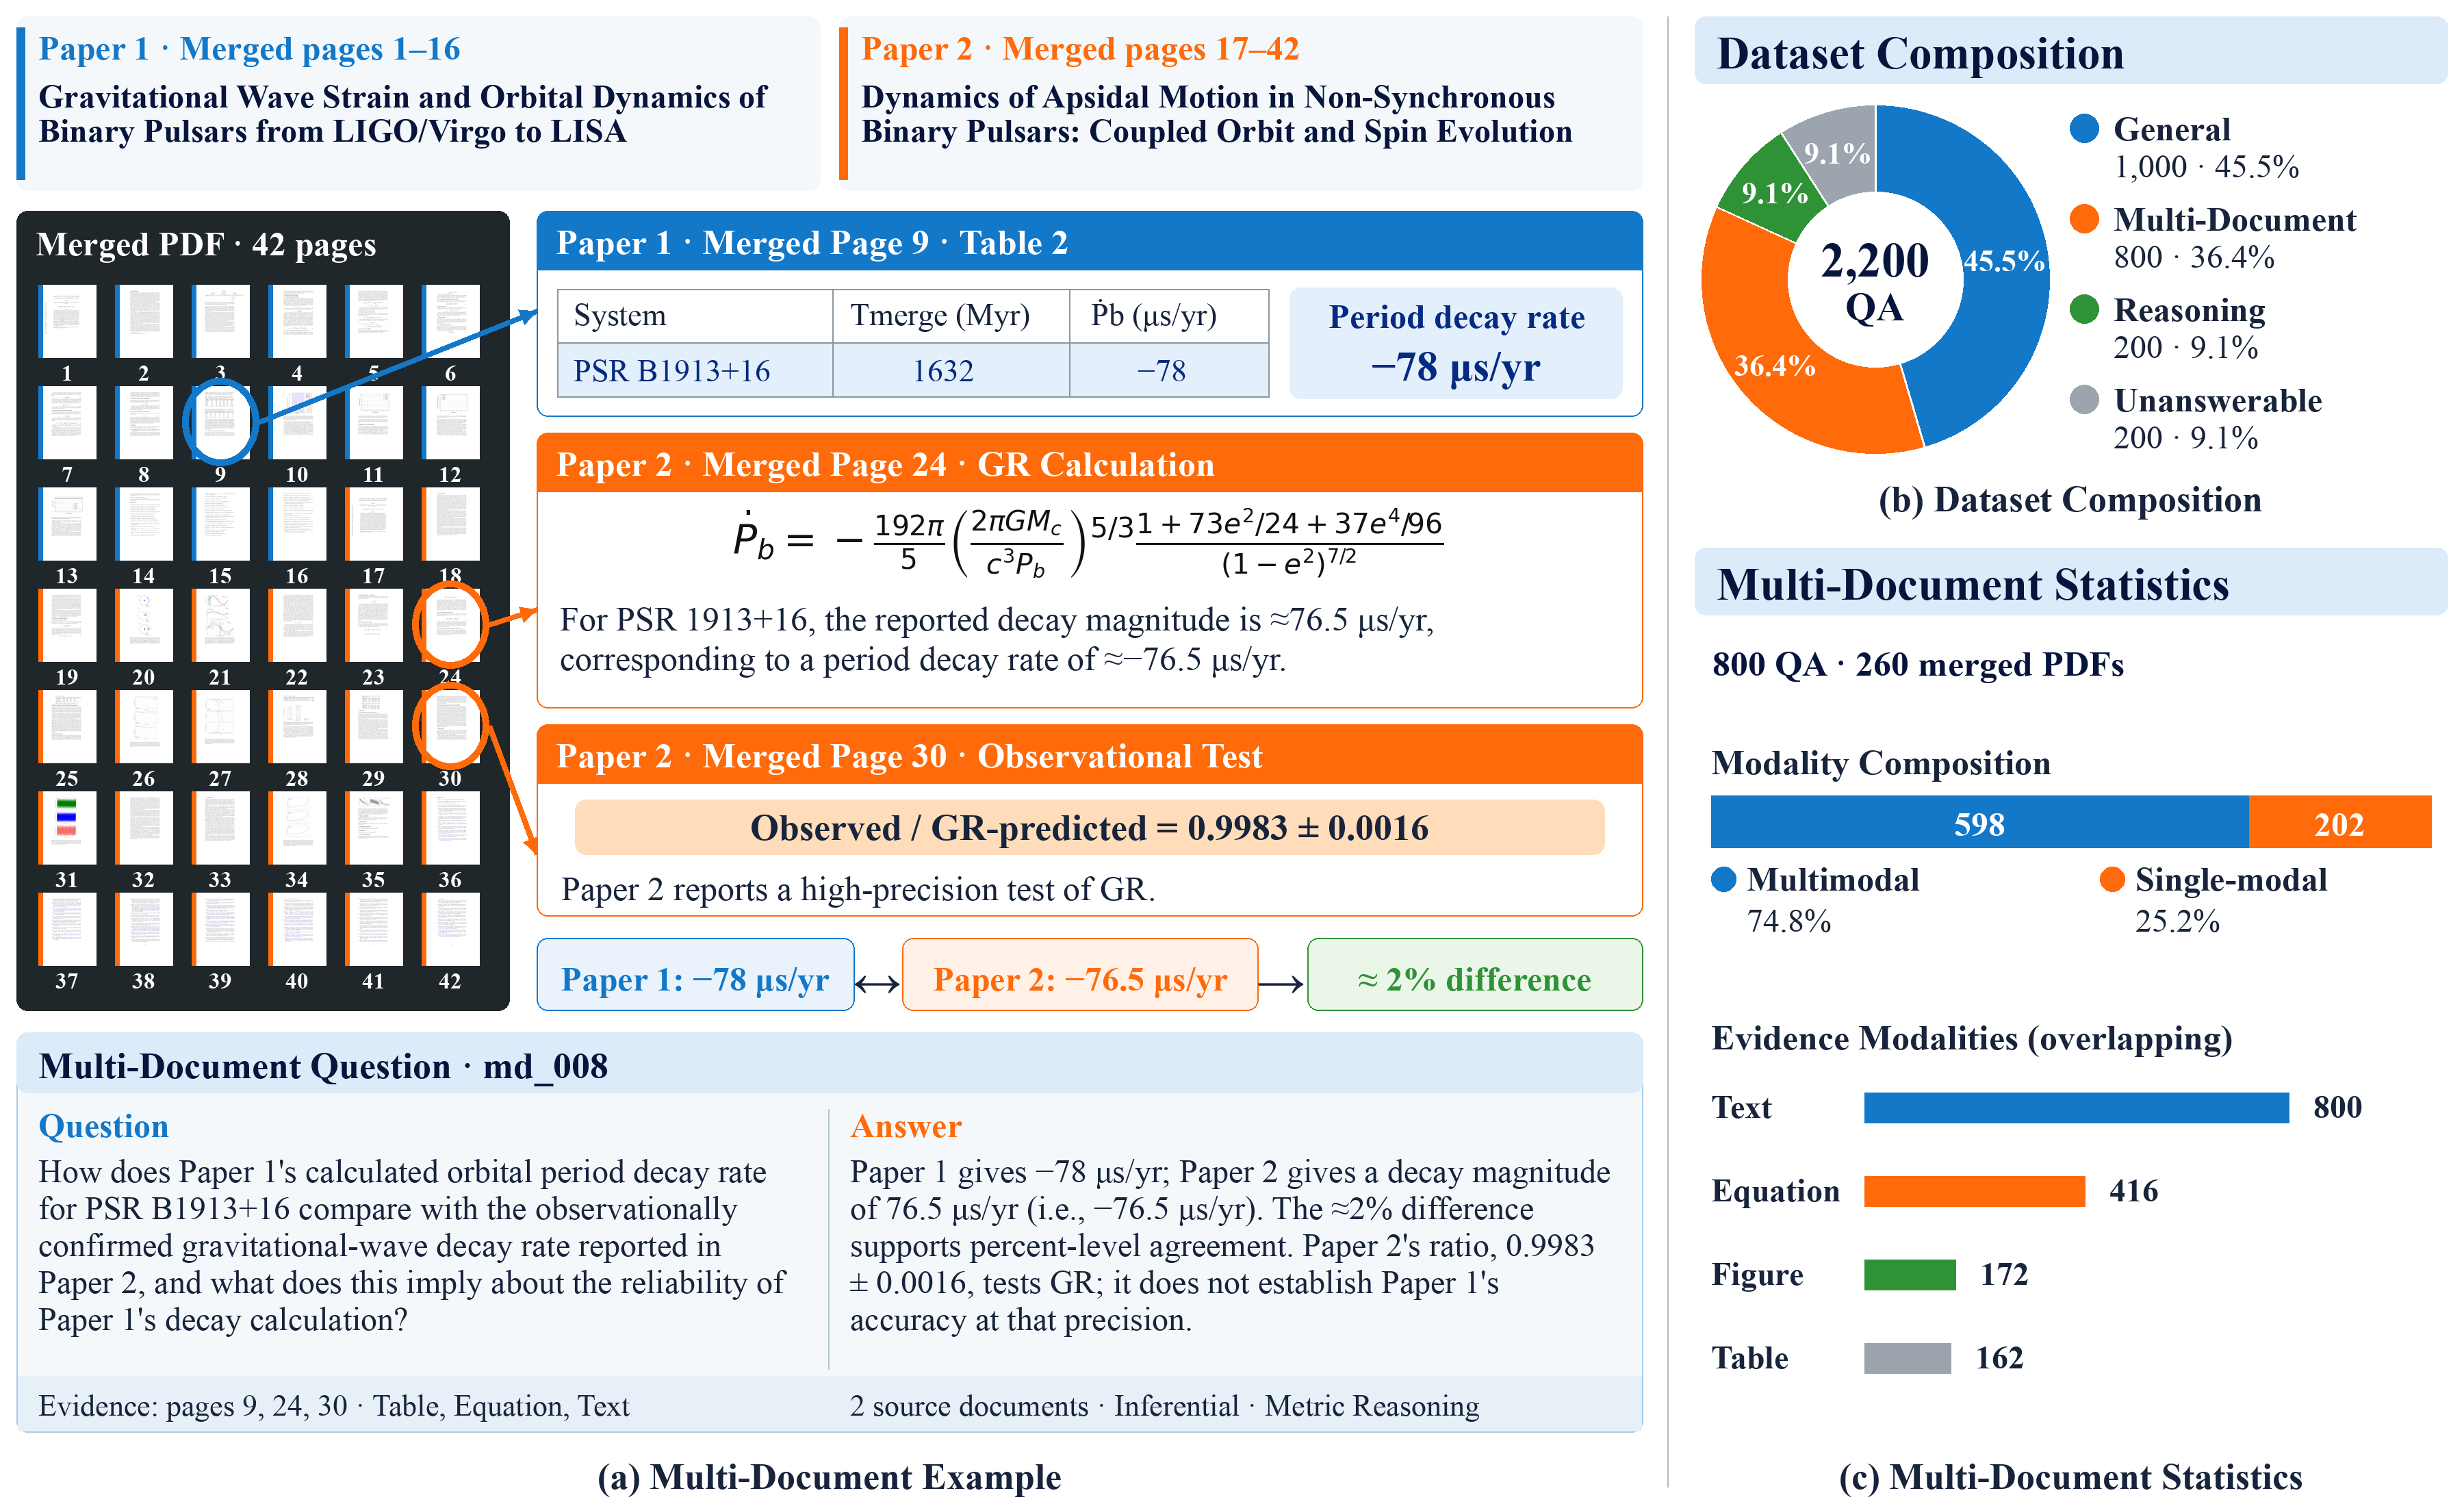
\includegraphics[width=\linewidth]{figures/fig_3_0_scidoc_overview.png}
    \caption{The multi-document question-answer example and dataset statistics.}
    \label{fig:scidoc_overview}
\end{figure}

Despite this progress, three challenges remain. First, scientific fields differ in their knowledge forms and reasoning patterns, making broad and discipline-aware evaluation necessary. Second, a correct answer does not always indicate correct document understanding, since models may rely on prior knowledge or incomplete evidence. Therefore, scientific QA requires explicit evaluation of evidence grounding. Third, scientific questions often require information from multiple pages, modalities, or documents, which makes cross-page and multi-document reasoning essential.

Accordingly, we propose ScienceDoc, an evidence-grounded multimodal question answering benchmark for scientific documents. ScienceDoc comprises 2,200 QA-pairs derived from 693 scientific documents, spanning 8 disciplines and 61 scientific fields.
%, covering \textit{Computer Science, Physics, Mathematics, Statistics, Quantitative Biology, Electrical Engineering and Systems Science, Economics, and Quantitative Finance}. 
The questions are manually designed according to discipline-specific requirements and verified to assess scientific understanding across text, equations, tables, and figures. ScienceDoc includes 1,000 General, 200 Unanswerable, 200 Reasoning, and 800 Multi-Document questions, covering 21 question types. Reasoning questions require integrating multiple pieces of evidence through comparison, causal reasoning, or multi-step calculation, while multi-document questions require combining complementary evidence from multiple documents. Each question is manually annotated with supporting evidence pages, enabling joint evaluation of answer correctness and evidence grounding. An example is shown in Figure~\ref{fig:scidoc_overview}.

Extensive evaluation of 11 MLLMs shows that ScienceDoc remains challenging for recent strong models.
Multi-document QA is particularly difficult, with 7 models achieving below 50\% accuracy, while performance on unanswerable questions varies widely from 2.5\% to 72.5\%, highlighting the difficulty of recognizing insufficient evidence. Performance also varies across scientific disciplines, and strong answer accuracy does not always correspond to precise evidence localization. These results show that ScienceDoc captures limitations in multi-document reasoning, insufficient-evidence recognition, domain robustness, and evidence grounding beyond conventional answer accuracy.

The main contributions are summarized as follows\footnote{All the code and dataset will be released upon acceptance.}:
1) We introduce ScienceDoc, a multidisciplinary scientific document QA benchmark covering 8 major disciplines, 61 scientific fields, 4 task types, 21 discipline-specific question types, and multiple modalities.
2) We provide expert-designed questions, expert-annotated answers, and evidence-page annotations, enabling joint evaluation of answer correctness and evidence grounding.
3) We benchmark 11 representative MLLMs under a unified protocol and provide detailed analysis of their performance across task types, scientific disciplines, multi-document reasoning, and evidence localization.

%Additional dataset representation and construction details are provided in Appendix~\ref{app:dataset_details}, while the complete quality-control and evaluation protocol is described in Appendix~\ref{app:detailed_protocol}.

\begin{table*}[t]
\centering
\caption{
Comparison of representative document understanding and scientific QA benchmarks.
Sci. Doc: scientific document; Modal.: modality; Multi. Doc.: multi-document;
Evid.: evidence annotation; Una.: unanswerable; DS Rea.: domain-specific reasoning;
Hie. Eval.: hierarchical evaluation.
T/Tb/Fg/Eq: text/table/figure/equation.
3S/26T: 3 subjects/26 topics; 8D/61F: 8 domains/61 scientific fields.
$\checkmark$/$\times$/$\triangle$: supported/unsupported/partially supported.
}
\label{tab:benchmark_comparison}

\resizebox{\textwidth}{!}{
\setlength{\tabcolsep}{3pt}
\renewcommand{\arraystretch}{1.15}

\begin{tabular}{
l
>{\centering\arraybackslash}m{1.35cm}
>{\centering\arraybackslash}m{1.45cm}
>{\centering\arraybackslash}m{1.65cm}
*{4}{>{\centering\arraybackslash}m{1.18cm}}
>{\centering\arraybackslash}m{1.85cm}
@{}
}
\toprule
\multirow{3}{*}{\textbf{Dataset}} &
\multicolumn{3}{c}{\textbf{Domain \& Modality}} &
\multicolumn{4}{c}{\textbf{Task Design}} &
\textbf{Evaluation} \\
\cmidrule(lr){2-4}
\cmidrule(lr){5-8}
\cmidrule(lr){9-9}

&
\textbf{Sci. Doc} &
\textbf{Sci. Domain} &
\textbf{Modal.} &
\textbf{Multi. Doc.} &
\textbf{Evid.} &
\textbf{Una.} &
\textbf{DS Rea.} &
\textbf{Hie. Eval.} \\
\midrule

DocVQA~\citep{mathew2021docvqa}
& $\times$
& --
& T/Tb/Fg
& $\times$
& $\times$
& $\times$
& $\times$
& $\times$ \\

QASPER~\citep{dasigi2021dataset}
& $\checkmark$
& NLP
& T/Tb/Fg
& $\times$
& $\checkmark$
& $\checkmark$
& $\times$
& $\times$ \\

ScienceQA~\citep{lu2022learn}
& $\times$
& 3S/26T
& T/Fg
& $\times$
& $\times$
& $\times$
& $\times$
& $\times$ \\

MP-DocVQA~\citep{tito2023hierarchical}
& $\times$
& --
& T/Tb/Fg
& $\times$
& $\checkmark$
& $\times$
& $\times$
& $\times$ \\

MMLongBench-Doc~\citep{ma2024mmlongbench}
& $\triangle$
& --
& T/Tb/Fg
& $\times$
& $\checkmark$
& $\checkmark$
& $\times$
& $\times$ \\

SPIQA~\citep{pramanick2024spiqa}
& $\checkmark$
& CS
& T/Tb/Fg
& $\times$
& $\checkmark$
& $\times$
& $\times$
& $\times$ \\

%M3SciQA~\citep{li2024m3sciqa}
%& $\checkmark$
%& NLP
%& T/Tb/Fg
%& $\checkmark$
%& $\checkmark$
%& $\times$
%& $\times$
%& $\times$ \\

LongDocURL~\citep{deng2025longdocurl}
& $\triangle$
& --
& T/Tb/Fg
& $\times$
& $\checkmark$
& $\times$
& $\times$
& $\checkmark$ \\

PaperScope~\citep{xiong2026paperscope}
& $\checkmark$
& AI
& T/Tb/Fg/Eq
& $\checkmark$
& $\checkmark$
& $\times$
& $\times$
& $\checkmark$ \\

\cellcolor{gray!15}\textbf{ScienceDoc (Ours)}
& \cellcolor{gray!15}$\checkmark$
& \cellcolor{gray!15}8D/61F
& \cellcolor{gray!15}T/Tb/Fg/Eq
& \cellcolor{gray!15}$\checkmark$
& \cellcolor{gray!15}$\checkmark$
& \cellcolor{gray!15}$\checkmark$
& \cellcolor{gray!15}$\checkmark$
& \multicolumn{1}{
    >{\columncolor{gray!15}[\tabcolsep][0pt]\centering\arraybackslash}
    m{1.85cm}@{}
  }{$\checkmark$} \\

\specialrule{\heavyrulewidth}{0pt}{0pt}
\end{tabular}}
\end{table*}

\section{Related Work}

\paragraph{Document Understanding}

Research in document understanding field has gradually evolved from single-page visual question answering to long-document, multi-page, and multimodal reasoning~\citep{han2025mdocagent,hu2025mplug}.
Early benchmarks such as DocVQA~\citep{mathew2021docvqa} focus on understanding text, layout, and visual content in document images. MP-DocVQA~\citep{tito2023hierarchical} extends this setting to multi-page documents, requiring models to retrieve relevant information from a larger page range before answering questions. More recent benchmarks further increase document length and reasoning complexity. MMLongBench-Doc~\citep{ma2024mmlongbench} evaluates long multimodal documents with text, figures, and tables, and includes cross-page and unanswerable questions. LongDocURL~\citep{deng2025longdocurl} further integrates long-document understanding, numerical reasoning, and content localization into a unified benchmark. These studies have significantly advanced long-context and multimodal document understanding~\citep{chia2025m,wang2025wilddoc}. However, their tasks mainly focus on general or professional documents and usually adopt domain-independent question designs. As a result, they do not capture the distinct reasoning patterns of scientific disciplines, such as equation-based reasoning in mathematics and physics or experiment-oriented reasoning in biology and statistics. In addition, existing benchmarks often evaluate individual abilities, such as answer generation or evidence retrieval, rather than providing a unified evaluation of multimodal understanding, refusal, complex reasoning, multi-document reasoning, and evidence grounding.

\paragraph{Scientific Question Answering}

Recent works have progressed from general science knowledge to the understanding of real scientific papers and reports~\citep{auer2023sciqa,wang2025charxiv,astaraki2026iterative}. ScienceQA~\citep{lu2022learn} introduces a large-scale multimodal benchmark covering natural science, social science, and language science, with questions mainly collected from educational scenarios. QASPER~\citep{dasigi2021dataset} moves scientific QA to research papers by introducing information-seeking questions over NLP papers together with supporting evidence annotations. Subsequent benchmarks further incorporate richer scientific content and more complex reasoning. SPIQA~\citep{pramanick2024spiqa} further incorporates figures, tables, and text from scientific papers and enables large-scale evaluation of multimodal scientific QA, with its data mainly drawn from computer science. More recently, PaperScope~\citep{xiong2026paperscope} constructs a multimodal document benchmark over AI papers and evaluates retrieval, reasoning, summarization, and problem solving in scientific literature. Although existing benchmarks have extended scientific QA to multimodal and long-document settings~\citep{wang2024t}, their disciplinary coverage remains limited, often focusing on NLP, computer science, or AI~\citep{lee2023qasa}. Moreover, their reasoning questions rarely reflect discipline-specific requirements, and existing evaluation frameworks lack a unified assessment of basic QA, unanswerable detection, discipline-specific reasoning, and evidence localization. These limitations hinder comprehensive evaluation of reliable scientific document understanding across diverse disciplines.

\begin{figure}[!t]
    \centering
    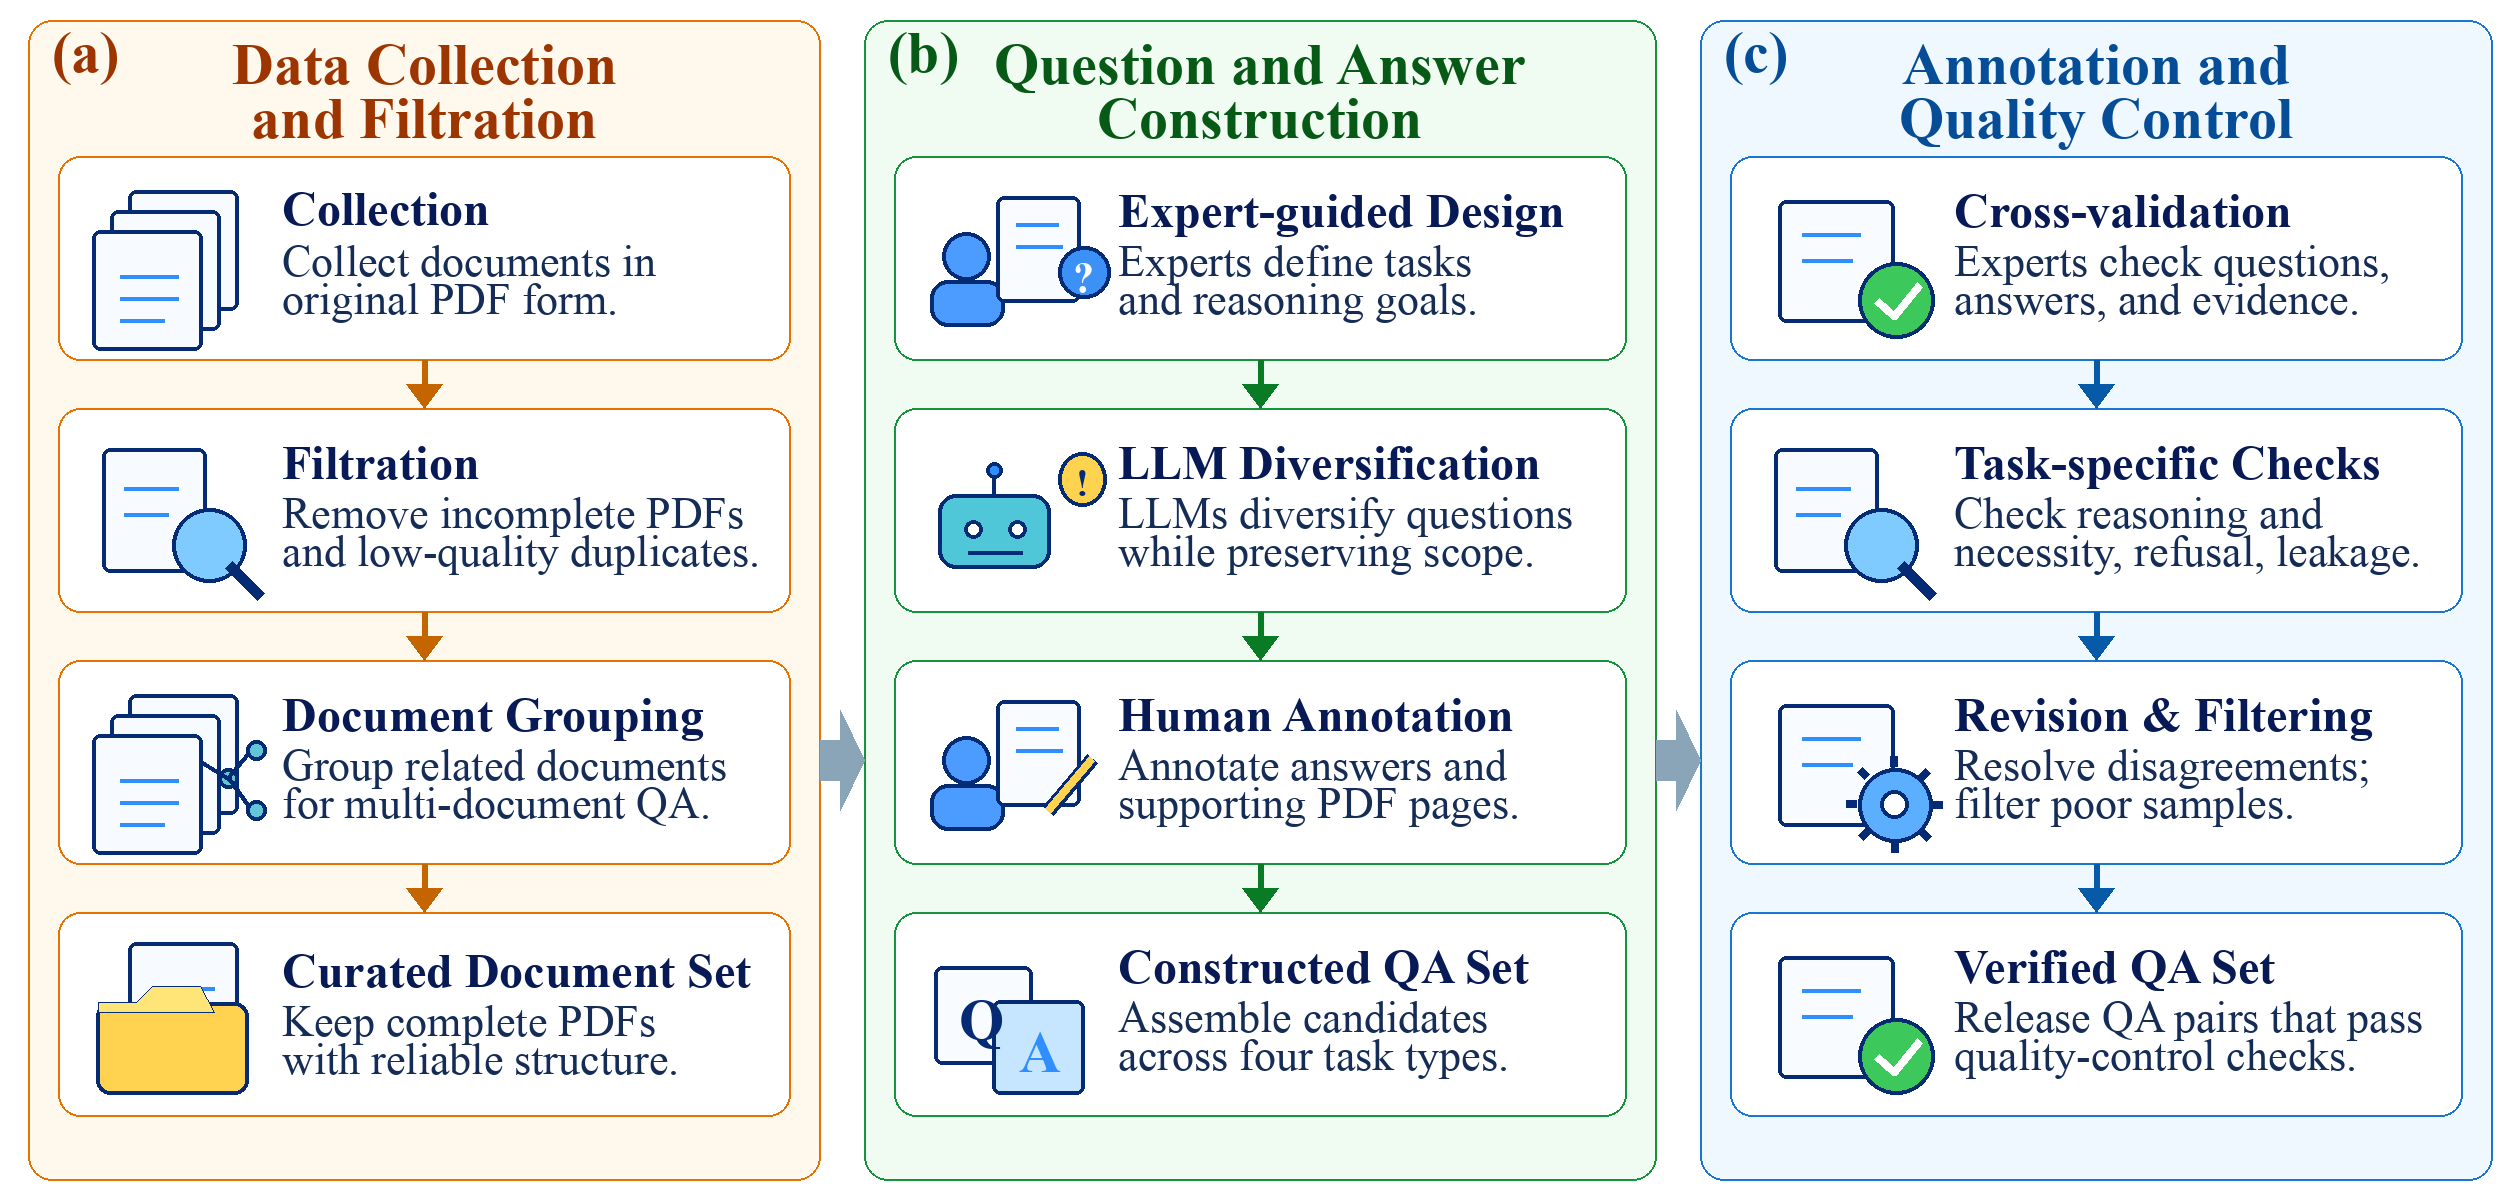
\includegraphics[width=\linewidth]{figures/fig_3_2_sci_doc_pipeline.png}
    \caption{Overview of the ScienceDoc dataset construction pipeline.}
    \label{fig:dataset_pipeline}
\end{figure}

%The qualitative study cases in Appendix~\ref{app:study_cases} further illustrate these document-understanding challenges.

\section{Dataset}
\label{sec:dataset}

%The proposed ScienceDoc is a multimodal scientific document QA benchmark built from original PDF documents, preserving text, equations, tables, figures, and page layouts. It covers 8 major disciplines and 61 scientific fields, with four question types: general, unanswerable, reasoning, and multi-document. The benchmark requires models to integrate information across pages and modalities, while multi-document questions further require evidence from multiple documents. All questions are designed by domain experts, with expert-annotated answers and manually labeled evidence pages, enabling joint evaluation of answer correctness and evidence grounding.

\subsection{Data Collection and Filtration}

\textbf{Document collection.} We collect scientific documents from multiple open-access sources, including arXiv, conference proceedings, and scientific journals. The collection spans 8 disciplines: \textit{Computer Science, Physics, Mathematics, Statistics, Quantitative Biology, Electrical Engineering and Systems Science, Economics, and Quantitative Finance}. Documents are retained in their original PDF format to preserve complete multimodal content and document structure. To reduce domain imbalance, we monitor the number of documents across both primary disciplines and fine-grained research areas and supplement underrepresented fields during collection. Figure~\ref{fig:dataset_pipeline} summarizes the overall construction pipeline of ScienceDoc.

\textbf{Document filtration.} We apply a multi-stage filtration process to ensure that the collected documents are suitable for multimodal scientific QA. The quality criteria considers 4 aspects: \textit{file integrity}, \textit{content completeness}, \textit{document quality}, and \textit{duplication}. We first remove files that could not be opened or parsed correctly, as well as documents containing missing, corrupted, or duplicated pages. We then examine document completeness, including the availability of the main body, figures, tables, equations, and experimental content when applicable. Documents with abnormal structures, extremely limited scientific content, or substantial rendering errors are excluded. Finally, we identify and remove duplicate publications, different versions of the same work, and highly overlapping documents based on their metadata and content. There are 693 documents that are retained after filtration. Figure~\ref{fig:dataset_domains} presents their distribution across the 8 disciplines and 61 scientific fields. Details in Appendix~\ref{app:paper_retrieval}.

\textbf{Multi-Document organization.} To construct the multi-document task, we organize two or three source documents into a document group according to their disciplinary relevance and potential information complementarity. We avoid grouping near-duplicate documents or documents whose content is largely redundant. Instead, each group is designed to contain distinct but related evidence that can support comparison, aggregation, or joint reasoning across sources. Candidate groups are further checked during question construction to ensure that each included document contributes necessary information to the corresponding question. This design reduces single-document shortcuts and requires models to identify and integrate evidence across document boundaries. Details in Appendix~\ref{app:cross_pdf_generation}.

\subsection{Question and Answer Construction}

\textbf{Expert-guided question design.} ScienceDoc adopts an expert-led and model-assisted construction paradigm. Rather than directly asking large language models to generate QA pairs from scientific documents, domain experts first define the discipline-specific question types and reasoning requirements for different disciplines. The design considers both the characteristics of scientific documents and the types of information commonly required in scientific reading, such as experimental settings, quantitative results, methodological details, equations, tables, figures, comparisons, and relationships between multiple pieces of evidence. Based on these criteria, experts manually construct the initial questions for each document and identify the information that should be required to answer them. This process ensures that the benchmark reflects meaningful scientific information needs rather than generic questions that can be produced from surface-level document content.

%\textbf{Model-assisted diversification.} Large language models were used only as an auxiliary tool to improve the diversity of expert-designed questions. Given an expert-designed question and its underlying information requirement, the model was instructed to generate alternative formulations or structurally varied versions while preserving the original scientific meaning, answer scope, and evidence dependency. The diversification process covers variations in wording, question structure, information presentation, and reasoning form, but does not allow the model to introduce unsupported scientific facts or change the intended answer. Domain experts subsequently screened the generated candidates and retained only questions that were semantically correct, natural, and consistent with the source documents. This expert-model collaboration increases linguistic and structural diversity while maintaining control over the scientific content and difficulty of the benchmark.

\textbf{Task types.} ScienceDoc contains 4 task types. \textit{General task} assesses information extraction and understanding across text, equations, tables, figures, and multiple pages. \textit{Unanswerable task} is semantically relevant to the document but cannot be answered using the available content, allowing us to evaluate whether models can recognize insufficient evidence rather than generate unsupported answers. Their reference answer is ``Unanswerable''. \textit{Reasoning task} requires combining multiple facts through comparison, conditional inference, multi-step calculation, constraint satisfaction, or causal reasoning, with questions solvable mainly by common knowledge or question cues excluded. \textit{Multi-Document task} requires complementary evidence from two or three documents, and each source must be necessary for deriving the final answer; otherwise, the question is revised or discarded. Construction details in Appendices~\ref{app:unanswerable_construction}--\ref{app:cross_pdf_generation}.

%\textit{Reasoning questions} require models to combine multiple facts through operations such as comparison, conditional inference, multi-step calculation, constraint satisfaction, or causal reasoning. \textit{Multi-Document questions} require evidence from two or three documents and are designed such that information from every included document is necessary for deriving the final answer. For reasoning questions, we preferentially construct questions whose supporting evidence is distributed across different document regions and remove questions that can be solved mainly through common knowledge or cues in the question itself. For multi-document questions, we further apply a source-necessity criterion: if the complete answer can still be derived after removing one of the source documents, the question is revised or discarded. This constraint ensures that multi-document questions evaluate genuine Multi-Document information integration rather than simple retrieval from one document.

\textbf{Answer construction.} ScienceDoc adopts a free-form answer format to reduce the possibility of models exploiting answer choices or other task-specific cues. Reference answers may contain numerical values, units, equations, lists, or concise textual descriptions. All final answers are manually annotated from the source documents rather than generated directly by models. Annotators also identify the minimum evidence set required to derive each answer, enabling the benchmark to evaluate both answer correctness and evidence grounding. More details in Appendices~\ref{app:page_representation}--\ref{app:construction_records}.

\subsection{Annotation and Quality Control}

\textbf{Professional annotation.} A total of 10 annotators participate in the professional annotation and cross-validation process. Annotators review the source documents and manually determine the reference answers and their supporting evidence. The annotation protocol emphasizes scientific precision, including numerical values, units, mathematical symbols, experimental conditions, comparison targets, and other context that could affect the interpretation of an answer. For questions involving multiple evidence sources, annotators are required to verify that the complete answer could be derived only when all necessary evidence is considered.

\textbf{Cross-validation.} Each QA instance is independently checked by at least two human experts. The reviewers verify 4 key aspects: question validity, answer correctness, evidence sufficiency, and evidence necessity. Specifically, they examine whether the question is clear and scientifically meaningful, whether the reference answer is fully supported by the document, whether the annotated evidence covers all information required to answer the question, and whether irrelevant evidence has been included. Questions with inconsistent annotations or reviewer disagreement are returned for further inspection and revision before inclusion in the final benchmark.

\textbf{Task-specific verification.} Additional checks are applied according to the task type. For reasoning questions, reviewers verify that the intermediate facts and reasoning dependencies are valid and that removing a required fact would prevent derivation of the complete answer. For multi-document questions, reviewers check the contribution of each source document and reject questions that could be answered using only a subset of the documents. For unanswerable questions, reviewers examine the complete source document to confirm that the required information is genuinely unavailable. We also remove questions containing direct answer leakage, excessive lexical cues, ambiguous conditions, incomplete evidence, or substantial semantic overlap with other questions.

\textbf{Manual review system.} To support consistent annotation and quality control, we develop an internal review interface that jointly presents the question, reference answer, evidence annotations, and source documents. Annotators can directly inspect the supporting content and revise or remove problematic samples. The system records annotation changes and review histories, allowing the complete construction process to remain traceable. Only QA instances that pass the required expert cross-validation are included in the final ScienceDoc benchmark. Review system in Appendices~\ref{app:dual_review}--\ref{app:final_freeze} and~\ref{app:pre_release}.

\begin{figure}[!t]
    \centering
    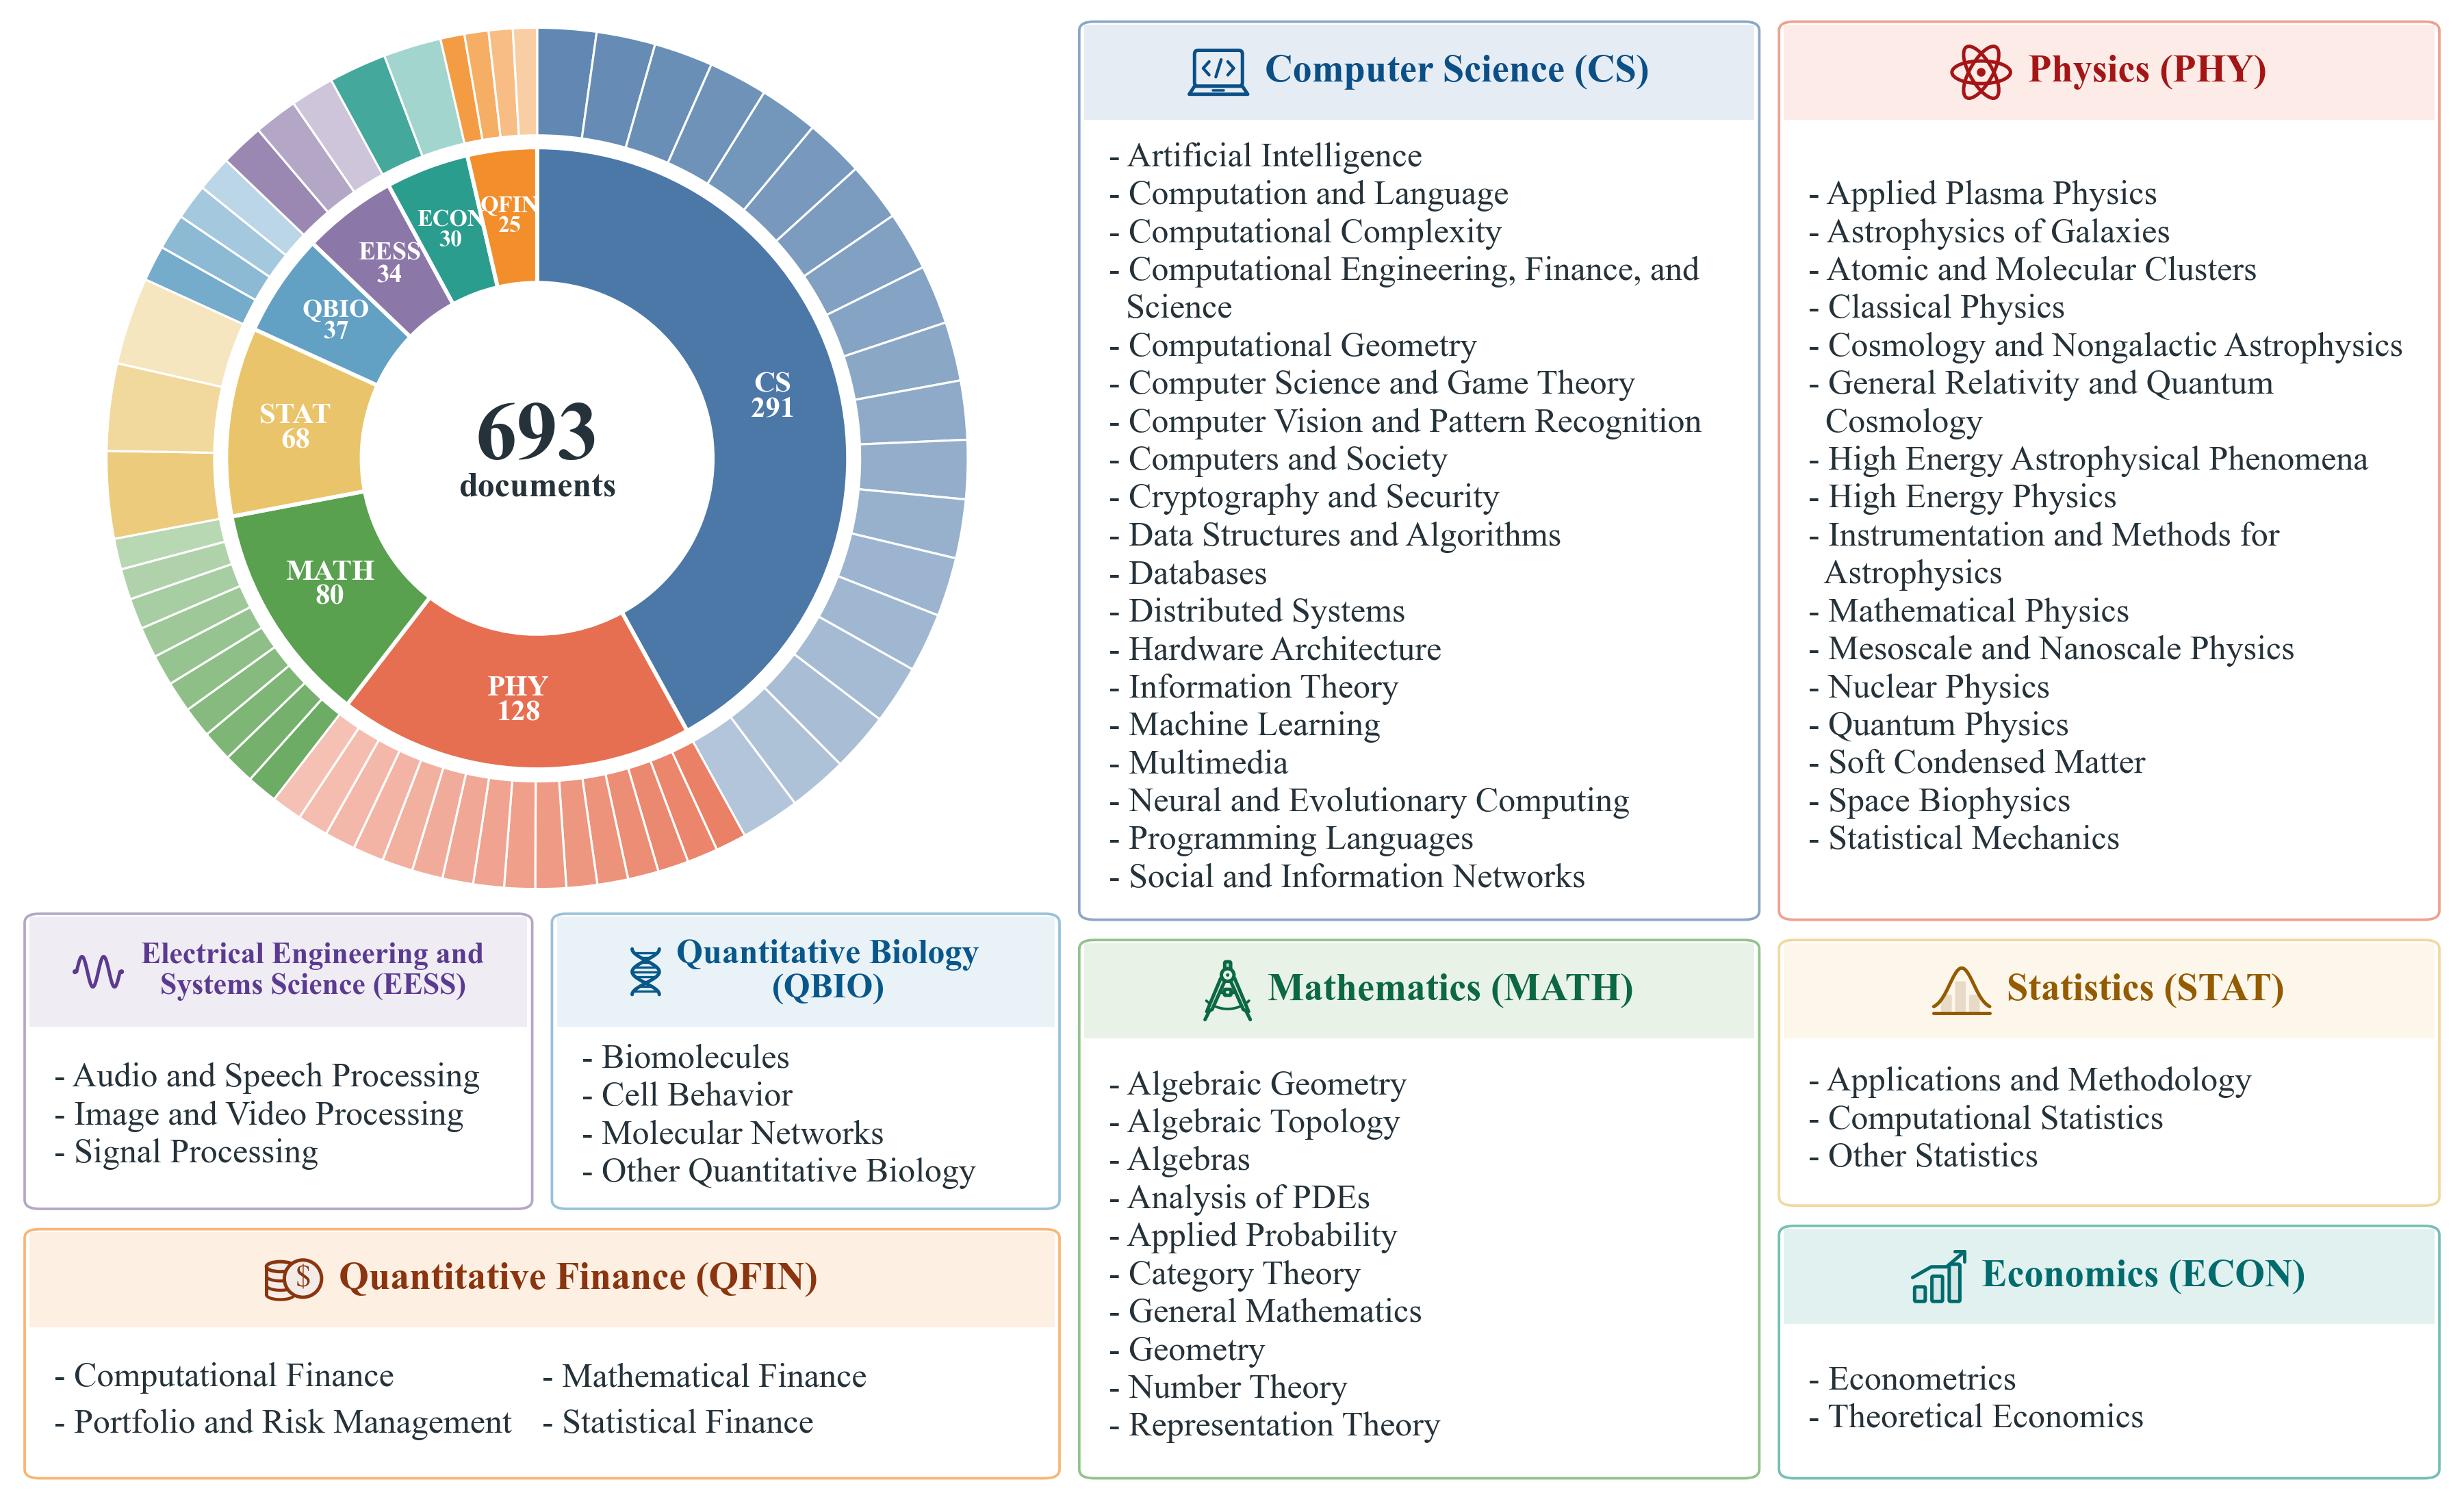
\includegraphics[width=\linewidth]{figures/fig_3_1_primary_domain_distribution.png}
    \caption{The disciplines and scientific fields of documents in ScienceDoc.}
    \label{fig:dataset_domains}
\end{figure}

\begin{figure}[!t]
    \centering
    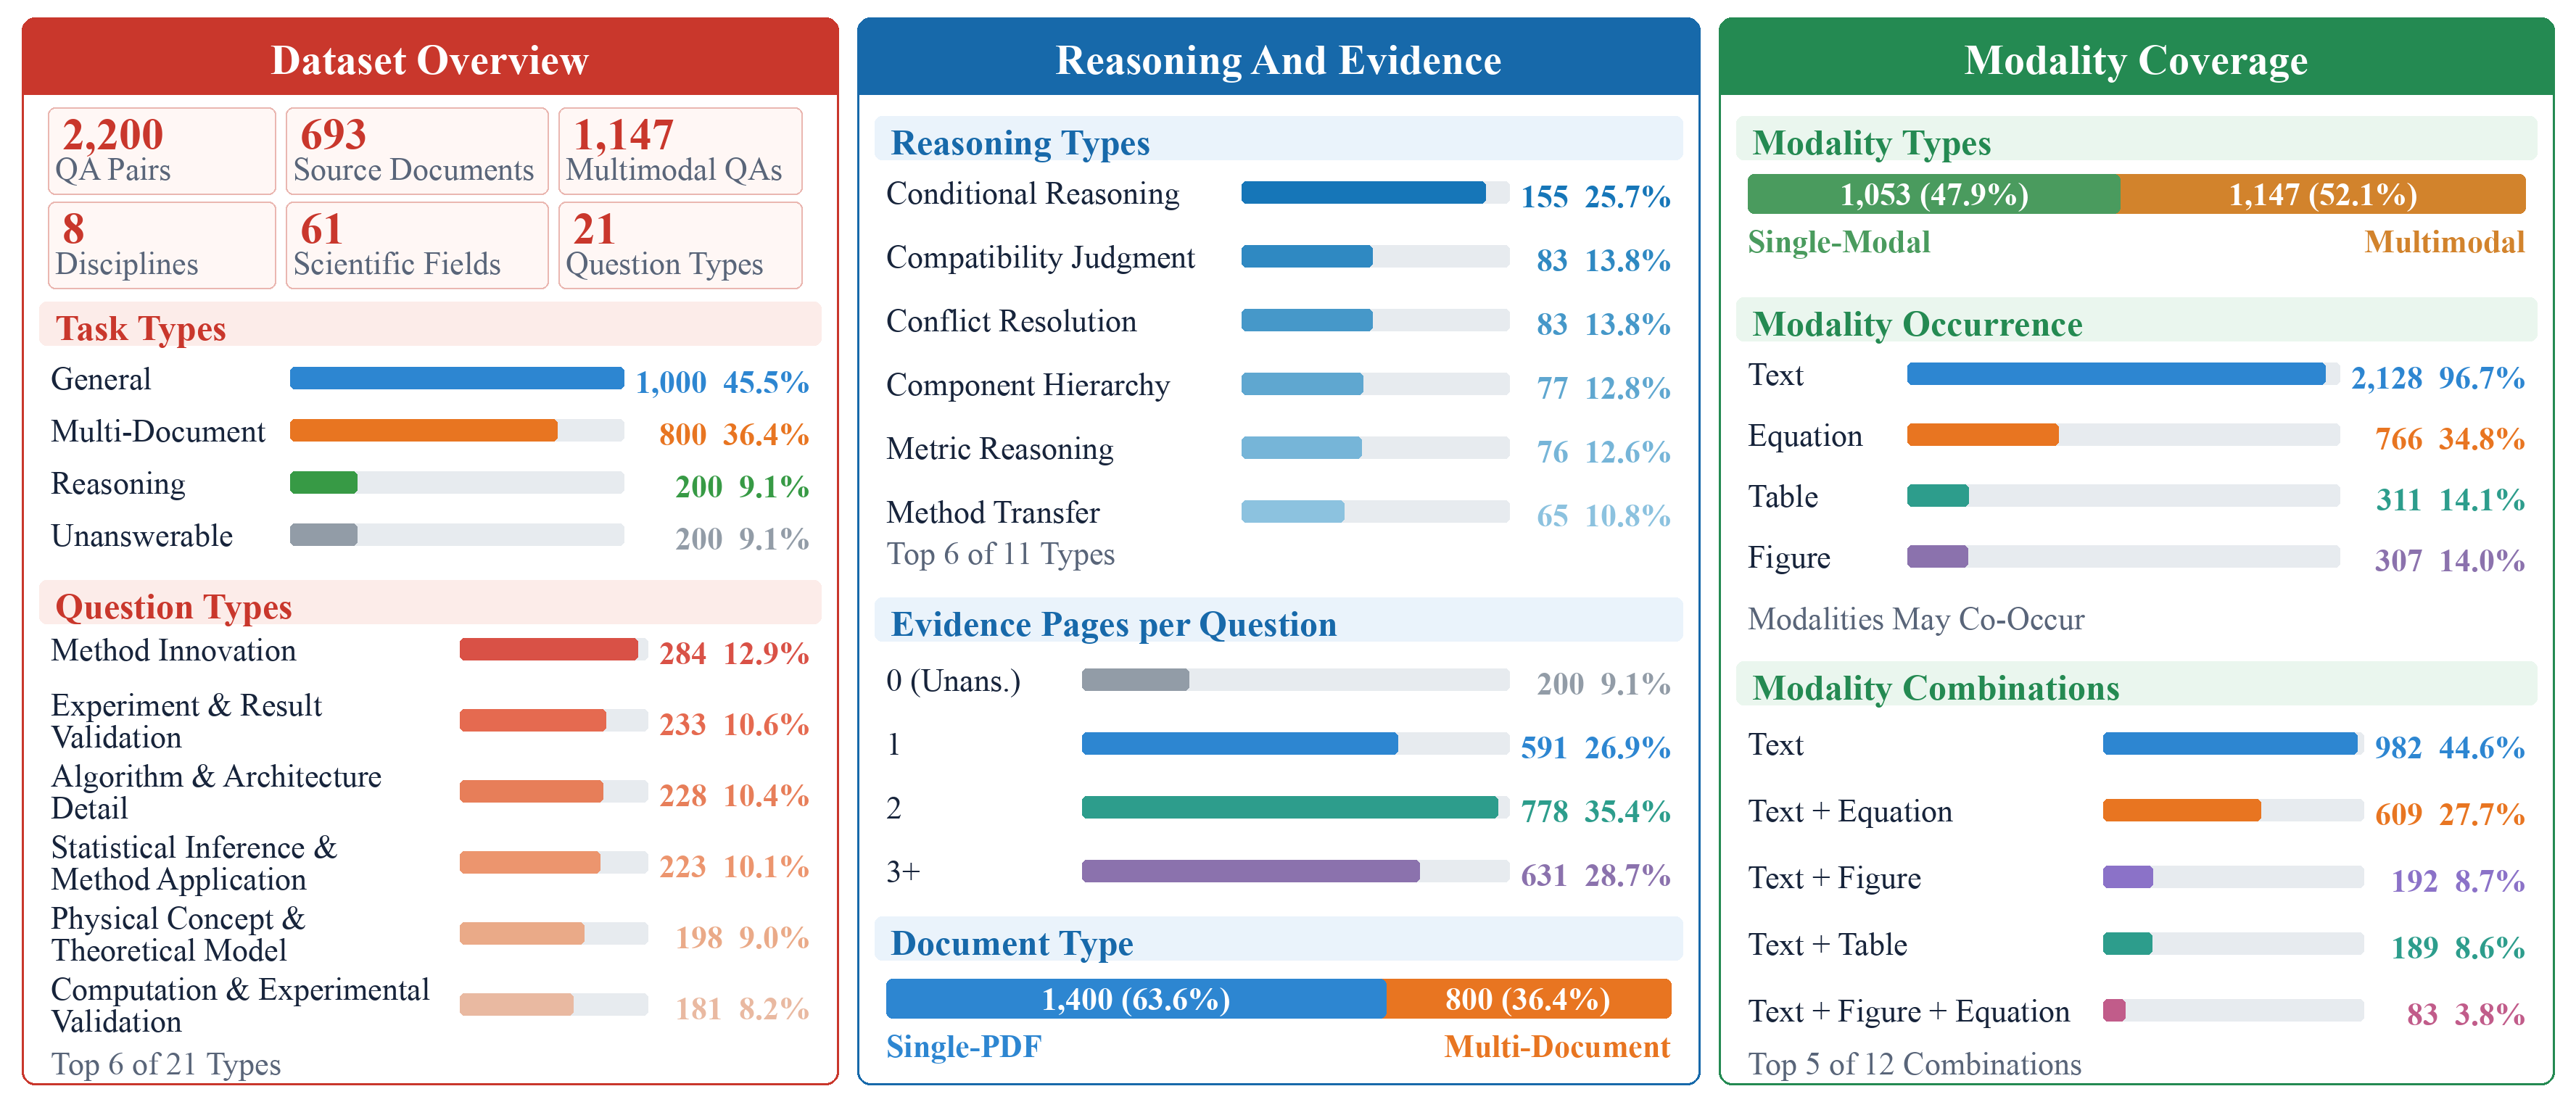
\includegraphics[width=\linewidth]{figures/fig_3_3_qa_composition.png}
    \caption{ScienceDoc statistics on question composition, reasoning and evidence, and modality.}
    %\caption{Question composition and coverage of ScienceDoc. Left: benchmark size, task families, answerability, and the six most frequent question categories. Center: the six leading annotated reasoning relations, evidence-page counts, document scope, evidence span, and source counts for Multi-Document questions. Right: modality profiles, modality occurrences, the five leading modality combinations, and question counts by discipline. Percentages use all 2,200 questions except reasoning relations (602 relation-labeled cases) and source counts (800 Multi-Document questions). Modality occurrences are non-exclusive; the displayed category, relation, and modality-combination rankings are partial lists. Zero evidence pages correspond to the 200 Unanswerable questions.}
    \label{fig:dataset_composition}
\end{figure}

\subsection{Dataset Statistics}

\textbf{Overall composition.} ScienceDoc contains 693 scientific documents and 2,200 questions, including 1,000 General questions (45.5\%), 200 Unanswerable questions (9.1\%), 200 Reasoning questions (9.1\%), and 800 Multi-Document questions (36.4\%), as shown in Figure~\ref{fig:dataset_composition}. Reasoning and Multi-Document questions together account for 45.5\% of the benchmark, providing substantial coverage of complex reasoning and information integration. The dataset spans 8 disciplines and 61 scientific fields (shown in Figure~\ref{fig:dataset_domains}), enabling broad evaluation of model performance across diverse scientific domains. Statistics and construction details in Appendices~\ref{app:dataset_statistics}--\ref{app:construction_lineage} and~\ref{app:construction_pipeline}.

\textbf{Question types and reasoning types.} Beyond the 4 task types, ScienceDoc includes 21 discipline-specific question types describing different scientific information needs. The most frequent are Method Innovation (284 questions), Experiment \& Result Validation (233), and Algorithm \& Architecture Detail (228). The dataset also contains 600 relation-labeled cases, with conditional inference being the most common (155; 25.8\%), followed by compatibility judgment and conflict resolution (83 each; 13.8\%). These relations characterize reasoning patterns and are not limited to the 200 reasoning questions, as they also occur in multi-document questions.

\textbf{Modality and evidence distribution.} ScienceDoc contains substantial multimodal and cross-page evidence. Among all questions, 876 (39.8\%) involve multiple modalities and 1,324 (60.2\%) involve a single modality. Text appears in 2,180 questions, equations in 349, tables in 322, and figures in 246, with overlapping counts for multimodal questions. Of the 2,000 answerable questions, 1,409 (70.5\%) require evidence from multiple pages, including all reasoning and multi-document questions. Moreover, 409 General questions also require cross-page evidence. These statistics highlight the need to evaluate evidence localization together with answer correctness. 

%Limitations in Appendix~\ref{app:data_card}.



%\textbf{Document organization.} For evaluation, the 693 source papers are organized into 734 PDF documents, including 474 single-paper PDFs and 260 merged PDFs containing two or three papers for Multi-Document evaluation. The Multi-Document subset involves 304 source papers, including 85 papers that also appear in the single-paper setting and 219 papers used only for Multi-Document questions.

%\textbf{Disciplinary coverage.} The questions span eight primary disciplines and 61 fine-grained fields (right panel of Figure~\ref{fig:dataset_composition}). At the question level, Computer Science contributes 743 items (33.8\%), followed by Physics with 379 (17.2\%), Statistics with 367 (16.7\%), and Mathematics with 245 (11.1\%). Economics, Electrical Engineering and Systems Science, Quantitative Biology, and Quantitative Finance contribute 137, 129, 114, and 86 items, respectively. Thus, 66.2\% of the questions lie outside Computer Science. This breadth supports evaluation across distinct scientific contexts, while the unequal question counts motivate reporting per-discipline performance alongside aggregate accuracy.

%\textbf{Question categories and reasoning relations.} Figure~\ref{fig:dataset_composition} complements the four task families with 21 question categories that describe scientific information needs. The most frequent categories are Method Innovation (283 questions), Experiment \& Result Validation (232), and Algorithm \& Architecture Detail (228). These categories describe question content rather than additional evaluation subsets. The figure also summarizes 602 relation-labeled cases, among which conditional inference is the most frequent relation (155; 25.7\%), followed by compatibility judgment and conflict resolution (84 each; 14.0\%). This relation-level summary uses its own denominator and should not be interpreted as a breakdown of only the 200 Reasoning questions.

%\textbf{Modality and evidence diversity.} As shown in the right panel of Figure~\ref{fig:dataset_composition}, 1,147 questions (52.1\%) involve multiple evidence modalities, while 1,053 (47.9\%) involve a single modality. Text occurs in 2,128 questions, equations in 766, tables in 311, and figures in 307; these occurrence counts overlap because a question may require several modalities. The leading exact modality combinations are text only (982), text with equations (609), text with figures (192), text with tables (189), and text with figures and equations (83), covering five of the 12 observed combinations. Among the 800 Multi-Document questions, 621 require information from two papers (77.6\%) and 179 from three papers (22.4\%). Together with the source-necessity checks described above, this composition supports evaluating integration of complementary evidence across modalities and documents.

%\textbf{Evidence distribution.} The center panel of Figure~\ref{fig:dataset_composition} summarizes the number of distinct annotated evidence pages across all questions; Figure~\ref{fig:app_dataset_statistics}(c) in Appendix~\ref{app:dataset_statistics} further breaks down this distribution by answerable task. Among the 2,000 answerable questions, 677 have a single annotated evidence page and 1,323 (66.2\%) require multiple evidence pages. These comprise 691 questions with two evidence pages and 632 with at least three. Cross-page evidence is not confined to the specialized subsets: 323 of the 1,000 General questions (32.3\%) also require more than one page. All Reasoning and Multi-Document questions have multiple evidence pages, with 130 of 200 Reasoning questions (65.0\%) and 481 of 800 Multi-Document questions (60.1\%) requiring at least three. The 200 Unanswerable questions have empty evidence sets and are excluded from these answerable-question statistics. The prevalence of distributed evidence motivates evaluating evidence localization alongside answer correctness, since models must identify the pages supporting different parts of an answer.

\FloatBarrier


\section{Experimental Setup}
\label{sec:experimental setup}

\textbf{Models:}
We evaluate 11 representative MLLMs to comprehensively assess current capabilities on our benchmark. For analysis and presentation, we divide the evaluated models into two scale groups:
\textit{Small-Scale Models} ($<10$B) and \textit{Large-Scale Models} ($>10$B). The evaluated small-scale models include Qwen3-VL-4B-Instruct and Qwen3-VL-8B-Instruct~\citep{bai2025qwen3}, InternVL3.5-8B~\citep{wang2025internvl3}, InternVL2.5-8B~\citep{chen2024expanding}, MiniCPM-V 4.5~\citep{yu2026minicpm}, and MiniCPM-V 2.6~\citep{yao2024minicpm}. We additionally evaluate large-scale models, including Mistral-Small-3.1-24B-Instruct-2503, Gemma 3 27B IT~\citep{team2025gemma}, GLM-4.6V~\citep{hong2025glm}, Claude Sonnet 5, and DeepSeek-V4-Flash-Vision-Exp(abbreviated as DeepSeek-V4-Flash thereafter)~\citep{xu2026deepseek}. These models span multiple model families and parameter scales, providing broad coverage of representative MLLMs. More details of models in Appendix~\ref{app:baselines}. 

\textbf{Settings:}
We evaluate all models under a unified input, prompting, and evaluation protocol. Each PDF is rendered at 144 DPI. All models are evaluated on a single NVIDIA A800 GPU, except for GLM-4.6V, Claude Sonnet 5, and DeepSeek-V4-Flash-Vision-Exp, which are accessed through their official APIs. Prompts and run settings in Appendices~\ref{app:prompts} and~\ref{app:reproduction}. 


\begin{table*}[t]
\centering
\caption{
Overall question answering and evidence localization performance.
All denotes accuracy over the complete benchmark; Gen.,
Unans., Multi-Doc., and Rea. denote general answerable QA,
unanswerable QA, Multi-Document QA, and reasoning QA, respectively.
Best and second-best results are shown in \textbf{bold} and
\underline{underline}, respectively.
}
\label{tab:main_evidence_results}

\setlength{\tabcolsep}{1.5pt}
\renewcommand{\arraystretch}{1.08}

\resizebox{\textwidth}{!}{
\begin{tabular}{M G C C C C C C C C}
\toprule

\multirow{3}{*}{\textbf{Model}}
&
\multicolumn{1}{c}{\multirow{3}{*}{\textbf{All}}}
&
\multicolumn{4}{c}{\textbf{Breakdown of Task Types (\%)}}
&
\multicolumn{4}{c}{\textbf{Evidence Localization}}
\\

\cmidrule(lr){3-6}
\cmidrule(lr){7-10}

&
\multicolumn{1}{c}{}
&
\makecell[c]{\textbf{Gen.}}
&
\textbf{Unans.}
&
\textbf{Multi-Doc.}
&
\textbf{Rea.}
&
\textbf{E-Prec.}
&
\textbf{E-Rec.}
&
\textbf{E-F1}
&
\textbf{A-Pages}
\\

\midrule

\multicolumn{10}{c}{\textbf{Small-Scale Models ($<$10 B)}} \\
\midrule

MiniCPM-V 2.6
& 15.59 & 14.70 & 38.50 & 12.50 & 9.50
& 9.37 & 9.24 & 9.26 & 0.11 \\

InternVL2.5-8B
& 22.32 & 24.40 & 32.00 & 14.25 & 34.50
& 15.39 & 31.88 & 16.75 & 6.69 \\

MiniCPM-V 4.5
& 34.32 & 54.60 & 15.00 & 10.75 & 46.50
& 20.03 & 15.92 & 16.47 & 1.42 \\

InternVL3.5-8B
& 34.95 & 36.30 & 2.50 & 36.88 & 53.00
& 30.86 & 31.20 & 28.04 & 3.72 \\

Qwen3-VL-4B
& 64.91 & 80.00 & \underline{60.00} & 47.38 & 64.50
& 39.35 & \textbf{53.01} & 39.22 & 9.26 \\

Qwen3-VL-8B
& 68.32 & 83.20 & 42.50 & 55.38 & 71.50
& 43.34 & 49.63 & 40.66 & 8.44 \\

\midrule

\multicolumn{10}{c}{\textbf{Large-Scale Models ($>$10 B)}} \\
\midrule

Gemma 3 27B
& 47.32 & 57.00 & 14.00 & 43.62 & 47.00
& 34.02 & 30.85 & 30.36 & 1.98 \\

Mistral-Small-3.1-24B
& 49.00 & 72.40 & 9.00 & 24.88 & 68.50
& 34.51 & 36.39 & 32.39 & 3.58 \\

Claude Sonnet 5
& 69.09 & 70.50 & \textbf{72.50} & 61.00 & \textbf{91.00}
& 36.26 & 44.56 & 37.10 & 3.66 \\

DeepSeek-V4-Flash
& \underline{79.45}
& \underline{88.20}
& 15.50
& \textbf{83.62}
& 83.00
& \underline{44.49}
& 49.22
& \underline{43.61}
& 2.57 \\

GLM-4.6V
& \textbf{80.95}
& \textbf{88.50}
& 46.00
& \underline{79.62}
& \underline{83.50}
& \textbf{51.04}
& \underline{50.47}
& \textbf{47.81}
& 1.97 \\

\bottomrule
\end{tabular}
}
\end{table*}


\begin{table*}[!t]
\centering
\caption{
Accuracy (\%) of different MLLMs across 8 disciplines.
CS, Phy., Stat., Math., Econ.,
EE, QBio., and QFin. denote Computer Science,
Physics, Statistics, Mathematics, Economics, Electrical Engineering and Systems Science,
Quantitative Biology, and Quantitative Finance, respectively.
Best and second-best results are shown in \textbf{bold} and
\underline{underline}, respectively.
}
\label{tab:subject_results}

\setlength{\tabcolsep}{1.5pt}
\renewcommand{\arraystretch}{1.08}

\resizebox{\textwidth}{!}{
\begin{tabular}{M G C C C C C C C C}
\toprule

\multirow{2}{*}{\textbf{Model}}
&
\multicolumn{1}{c}{\multirow{2}{*}{\textbf{All}}}
&
\multicolumn{4}{c}{\textbf{Fundamental \& Computational Sciences}}
&
\multicolumn{4}{c}{\textbf{Applied \& Interdisciplinary Sciences}}
\\

\cmidrule(lr){3-6}
\cmidrule(lr){7-10}

&
\multicolumn{1}{c}{}
&
\textbf{CS}
&
\textbf{Phy.}
&
\textbf{Stat.}
&
\textbf{Math.}
&
\textbf{EE}
&
\textbf{Econ.}
&
\textbf{QBio.}
&
\textbf{QFin.}
\\

\midrule

\multicolumn{10}{c}{\textbf{Small-Scale Models ($<$10 B)}} \\
\midrule

MiniCPM-V 2.6
& 15.59 & 16.51 & 18.73 & 15.85 & 10.20
& 10.16 & 16.06 & 15.79 & 15.12 \\

InternVL2.5-8B
& 22.32 & 21.34 & 26.39 & 24.32 & 13.88
& 17.97 & 32.12 & 19.30 & 23.26 \\

MiniCPM-V 4.5
& 34.32 & 25.91 & 44.85 & 33.88 & 30.20
& 30.47 & 40.88 & 51.75 & 46.51 \\

InternVL3.5-8B
& 34.95 & 37.99 & 30.34 & 36.07 & 20.82
& 38.28 & 43.80 & 36.84 & 43.02 \\

Qwen3-VL-4B
& 64.91 & 63.89 & 71.24 & 55.46 & 62.04
& 64.06 & 67.88 & \underline{80.70} & 69.77 \\

Qwen3-VL-8B
& 68.32 & 67.11 & 70.98 & 66.12 & 62.45
& 71.88 & 70.80 & 76.32 & 73.26 \\

\midrule

\multicolumn{10}{c}{\textbf{Large-Scale Models ($>$10 B)}} \\
\midrule

Gemma 3 27B
& 47.32 & 50.34 & 51.72 & 47.81 & 32.24
& 41.41 & 57.66 & 38.60 & 46.51 \\

Mistral-Small-3.1-24B
& 49.00 & 40.13 & 60.95 & 45.08 & 45.71
& 50.78 & 63.50 & 64.91 & 52.33 \\

Claude Sonnet 5
& 69.09 & 70.07 & 71.50 & 60.11 & 61.22
& \underline{80.47} & 73.72 & 79.82 & 72.09 \\

DeepSeek-V4-Flash
& \underline{79.45}
& \underline{80.54}
& \underline{77.57}
& \textbf{83.06}
& \underline{71.84}
& 79.69
& \underline{83.94}
& 78.95
& \underline{77.91} \\

GLM-4.6V
& \textbf{80.95}
& \textbf{80.67}
& \textbf{82.59}
& \underline{80.05}
& \textbf{74.29}
& \textbf{85.16}
& \textbf{86.86}
& \textbf{82.46}
& \textbf{81.40} \\

\bottomrule
\end{tabular}
}
\end{table*}

\textbf{Evaluation:}
Our benchmark evaluates both answer correctness and evidence localization. 
Because semantically equivalent answers may differ substantially in wording and formatting, we do not rely on exact string matching. 
Following existing studies~\citep{zheng2023judging,liu2023g,zhu2025judgelm}, we use the LLM-as-a-Judge method to compare each prediction against the reference answer.
For Unanswerable QA, a response is correct only if the model correctly determines that the answer cannot be derived from the provided documents.
We further evaluate evidence localization using \textbf{E\_Precision}, \textbf{E\_Recall}, and \textbf{E\_F1}, corresponding to precision, recall, and F1 score computed over PDF page indices. We also report \textbf{A\_Pages}, the average number of unique pages selected as evidence.
Inference and scoring details in Appendices~\ref{app:inference_protocol}--\ref{app:judge_reporting}.


\section{Results}
\label{sec:results}

\subsection{Main Results}

\textbf{Overall accuracy generally improves with model scale, while ScienceDoc remains challenging across different model sizes.}
As shown in Table~\ref{tab:main_evidence_results}, larger models generally achieve higher overall accuracy, with GLM-4.6V and DeepSeek-V4-Flash-Vision reaching 80.95\% and 79.45\%, respectively. Among models below 10B parameters, the Qwen3-VL series performs particularly well: Qwen3-VL-4B and Qwen3-VL-8B achieve 64.91\% and 68.32\%, respectively, outperforming several larger models. However, none of the evaluated models below 10B exceeds 70\% accuracy, indicating that ScienceDoc remains challenging for smaller MLLMs despite recent advances.

\textbf{Performance varies substantially across task types, revealing distinct challenges in multi-document integration, reasoning, and unanswerable-question recognition.}
General questions are comparatively easier for most models, with the strongest models exceeding 80\% accuracy. multi-document questions remain more challenging: 7 of the 11 models achieve below 50\% accuracy, indicating difficulty in integrating complementary evidence across independent documents. Reasoning performance also varies widely, showing large differences in the ability to combine multiple pieces of evidence through multi-step reasoning. Unanswerable questions exhibit a particularly uneven pattern, with accuracy ranging from 2.50\% to 72.50\%. Several models that perform strongly on answerable questions achieve much lower accuracy on unanswerable subset, suggesting that recognizing when the available documents do not provide sufficient evidence is a distinct capability. We present case study in Appendix~\ref{app:study_cases}.

\textbf{Models achieve lower scores on evidence localization than on answer correctness while they differ significantly in the selection of supporting pages.}
As shown in Table~\ref{tab:main_evidence_results}, GLM-4.6V achieves the highest Evidence F1 of 47.81\%, while most models remain below 40\%, despite substantially higher answer accuracy. This gap indicates that generating correct answers does not necessarily imply accurate identification of supporting evidence. Models also exhibit different evidence-selection strategies. Qwen3-VL-4B and Qwen3-VL-8B retrieve 9.26 and 8.44 pages per question on average, achieving higher recall but lower precision. In contrast, GLM-4.6V and DeepSeek-V4-Flash retrieve fewer pages while achieving higher Evidence F1 scores. These results highlight the importance of precise evidence localization over broad retrieval for reliable scientific document QA. Further case studies and error analysis are provided in Appendices~\ref{app:study_cases} and~\ref{app:error_analysis}.


\subsection{Findings and Analysis}
\label{sec:findings}

\begin{figure}[t]
    \centering

    % ---------------------------------------------------------
    % (a) Answer Accuracy vs. Evidence Grounding
    % ---------------------------------------------------------
    \begin{subfigure}[t]{0.43\columnwidth}
        \centering
        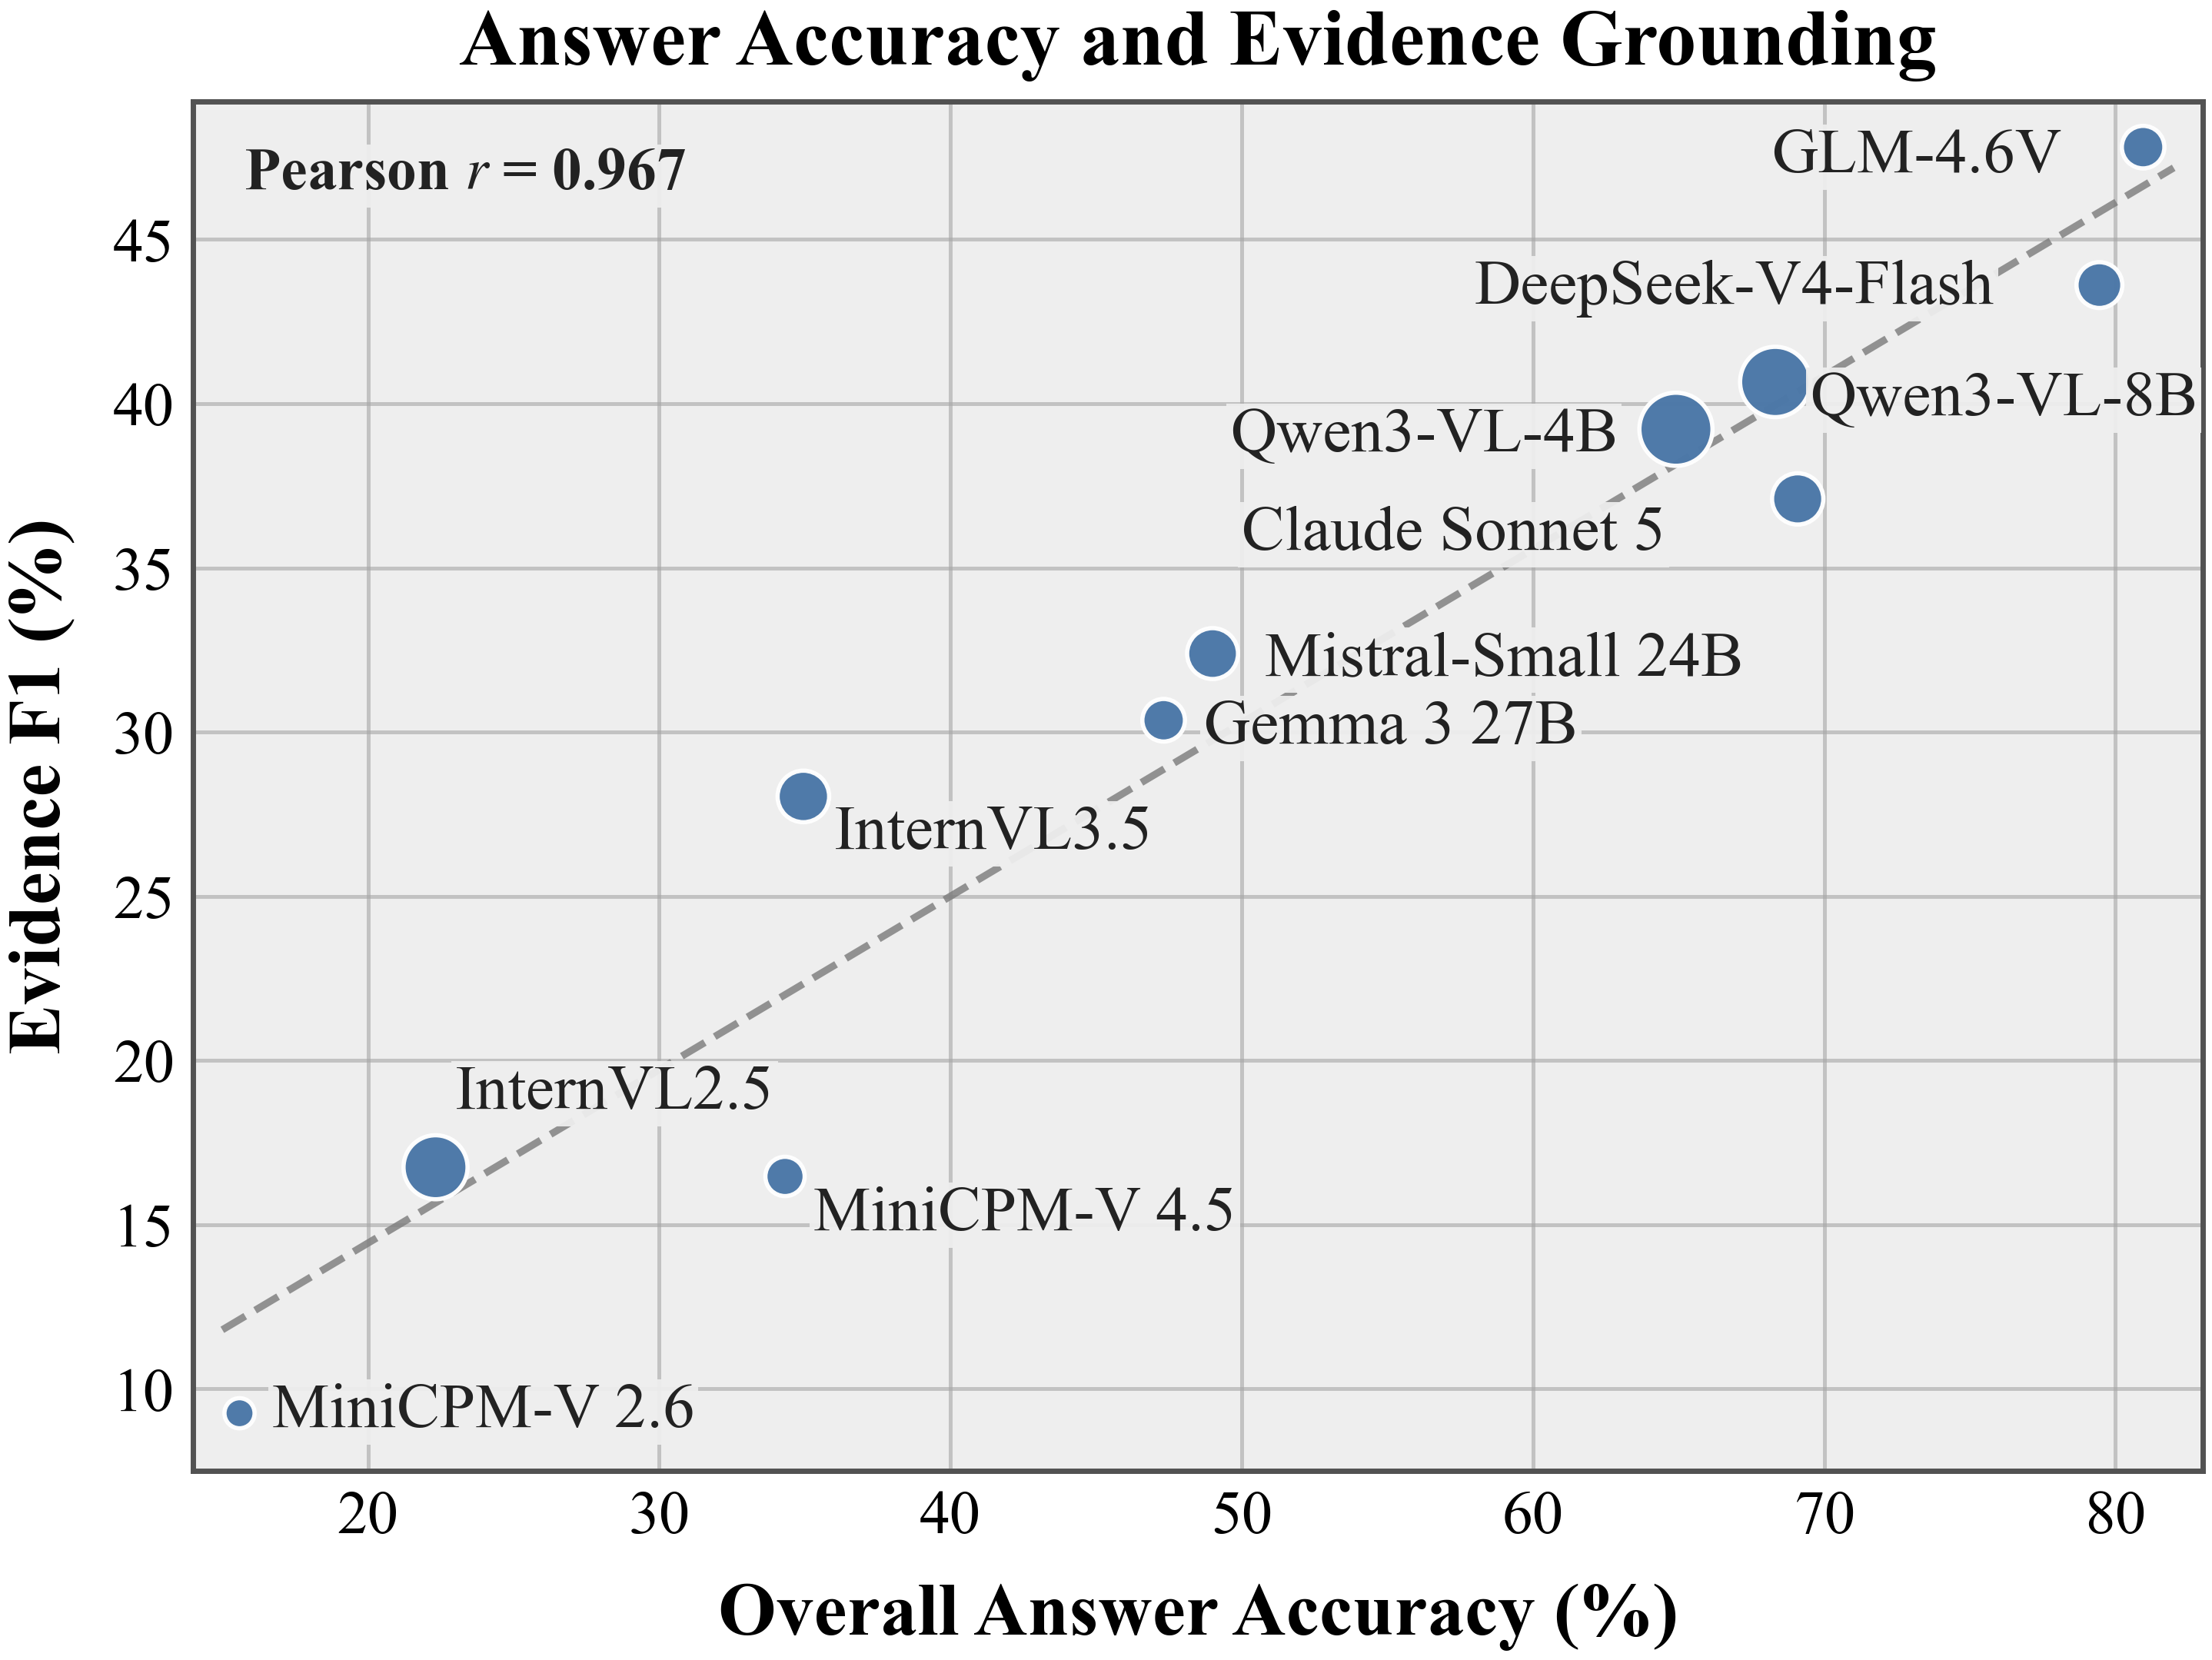
\includegraphics[
            width=\linewidth
        ]{figures/fig_answer_accuracy_vs_evidence_f1.png}
        \caption{
        Answer accuracy versus evidence grounding. Marker size indicates the average number of predicted evidence pages.
        }
        \label{fig:accuracy_evidence}
    \end{subfigure}
    \hfill
    % ---------------------------------------------------------
    % (b) Relative Domain Performance
    % ---------------------------------------------------------
    \begin{subfigure}[t]{0.55\columnwidth}
        \centering
        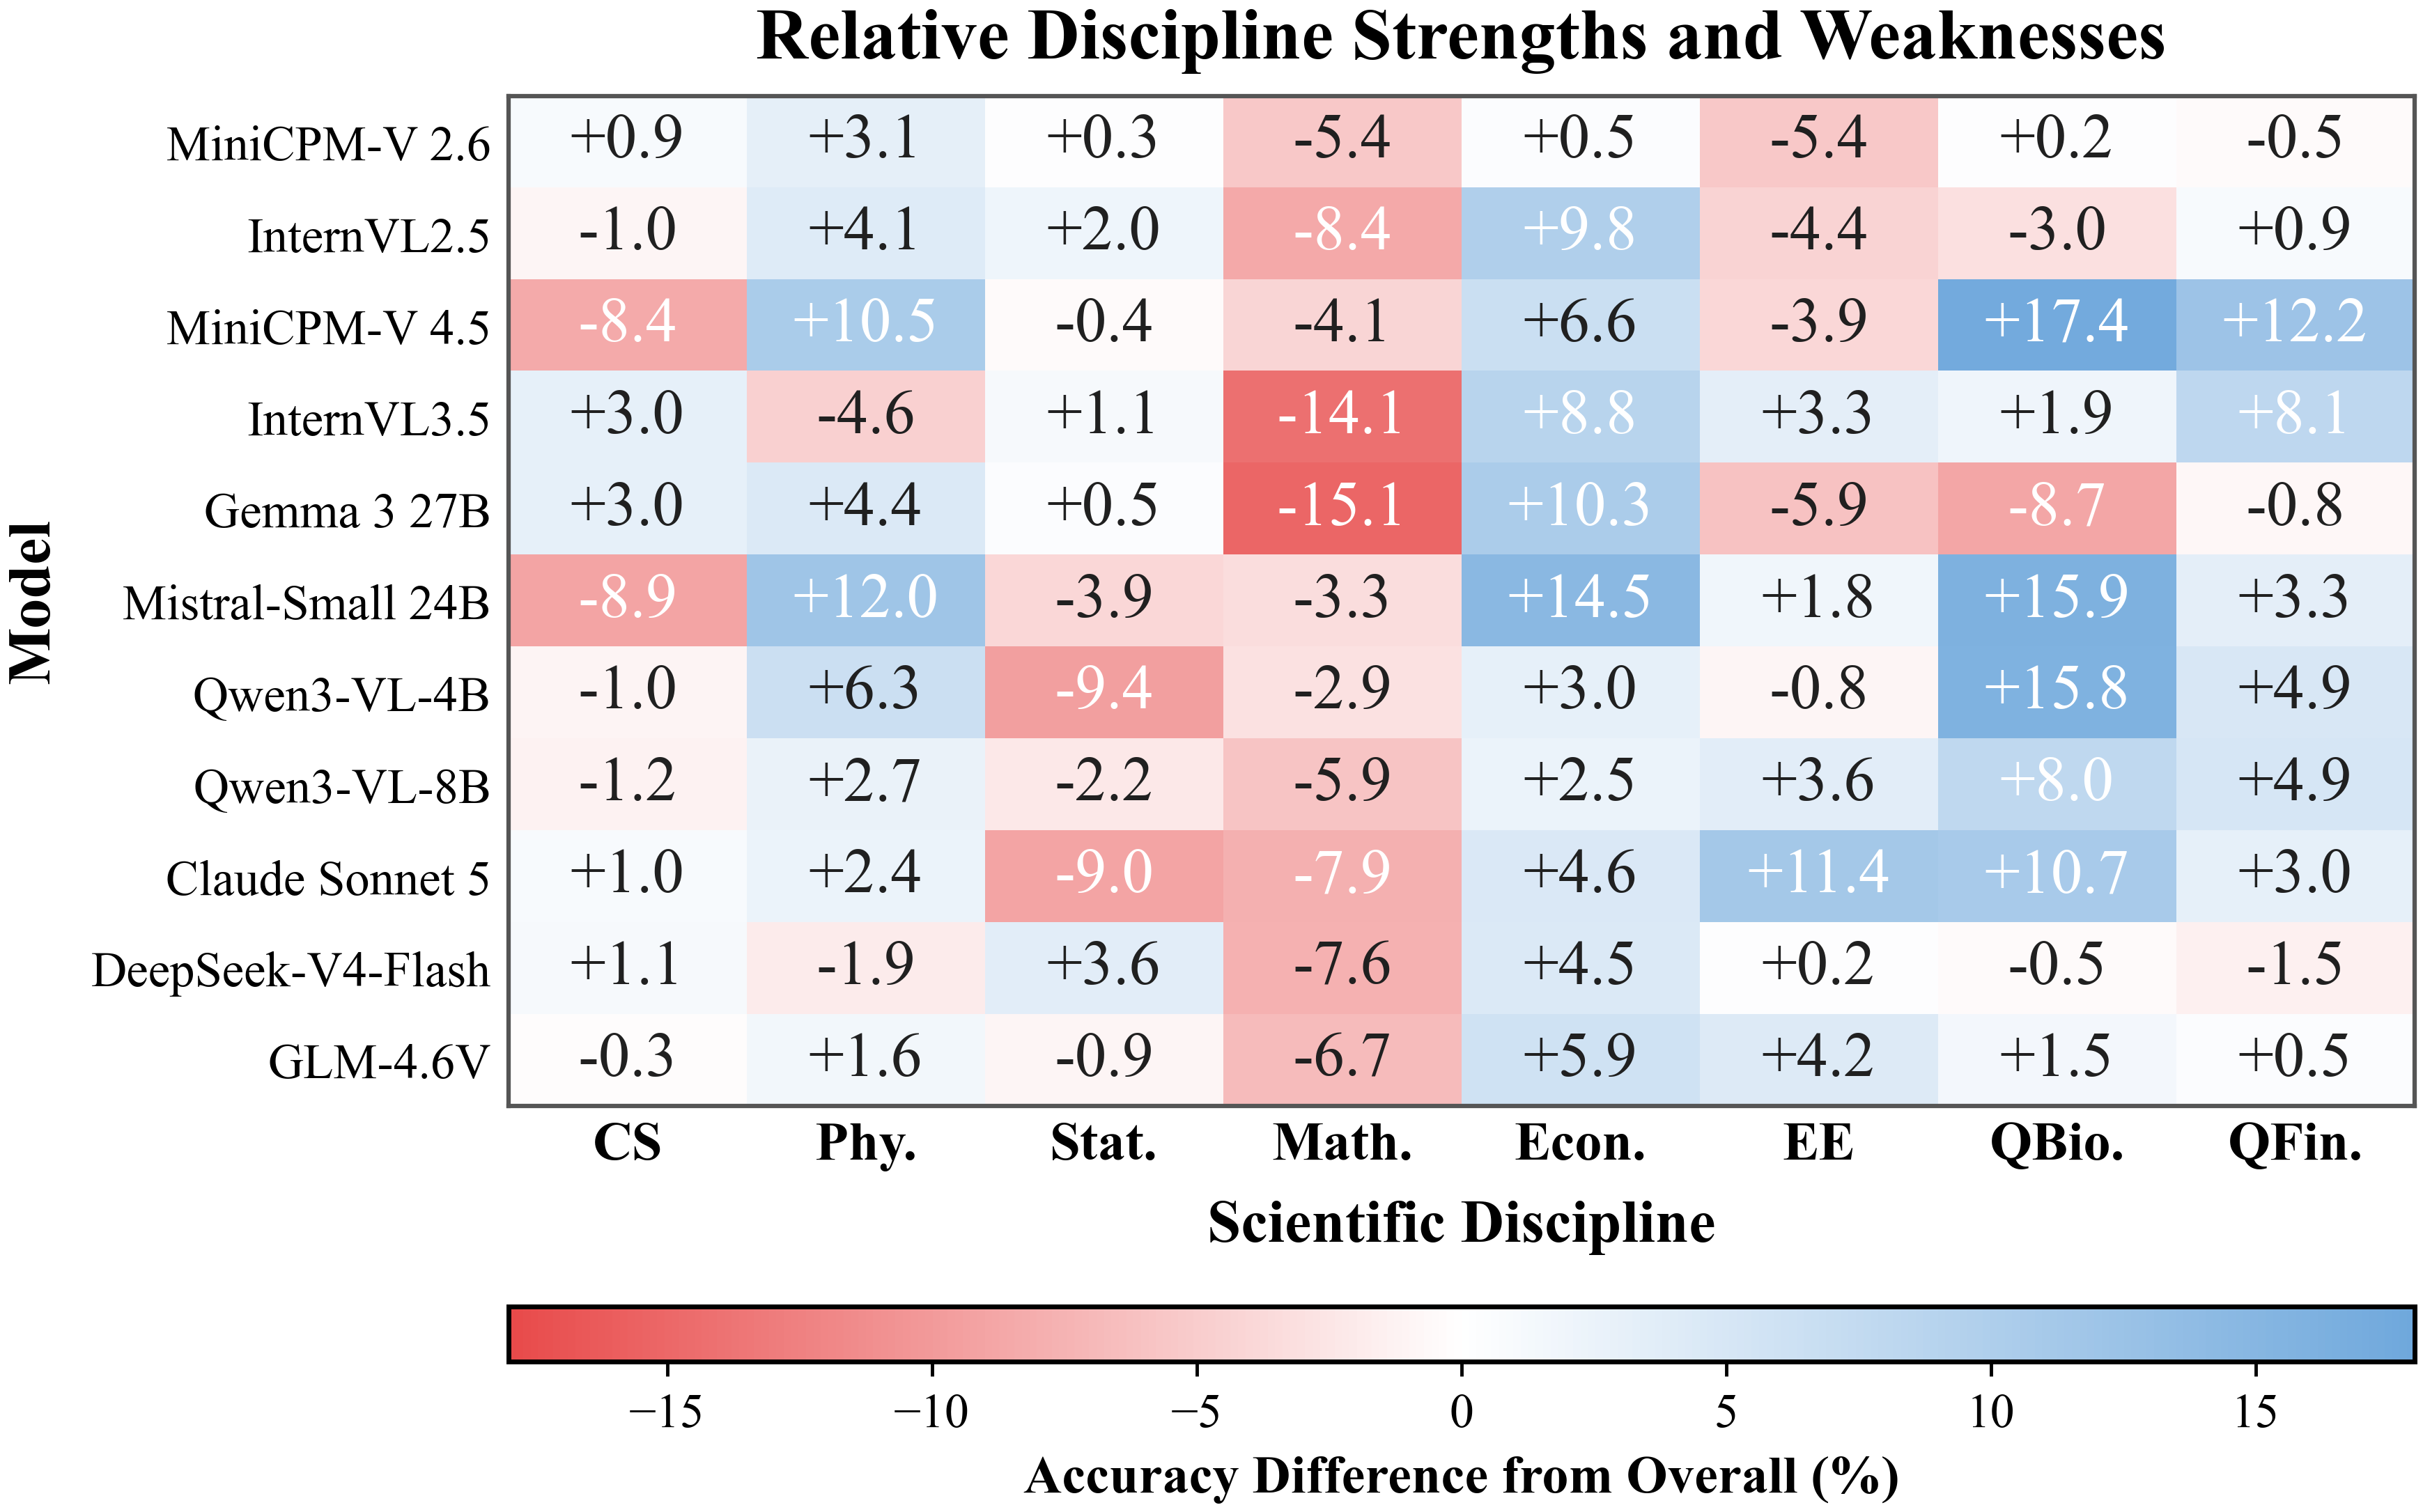
\includegraphics[
            width=\linewidth
        ]{figures/fig_relative_domain_heatmap.png}
        \caption{
        Model-specific relative strengths and weaknesses across 8 disciplines. Cell values are subject accuracy minus the model's overall accuracy.
        }
        \label{fig:domain_relative}
    \end{subfigure}

    \caption{
    Analysis of model performance in evidence grounding and across scientific disciplines.
    }
    \label{fig:findings}
\end{figure}


\textbf{Model performance varies substantially across scientific disciplines.}
Table~\ref{tab:subject_results} shows that the overall model ranking remains broadly consistent across disciplines, with GLM-4.6V and DeepSeek-V4-Flash-Vision leading overall and the Qwen3-VL series performing strongest among small-scale (below 10B) models.
However, the relative-performance heatmap in Fig.~\ref{fig:domain_relative} reveals noticeably different domain profiles across models.
Mathematics is the most consistent relative weakness, with all evaluated models performing below their own overall accuracy, whereas Physics, Economics, and Quantitative Biology frequently emerge as relative strengths.
These variations indicate that similar aggregate accuracy can mask substantially different patterns of discipline-specific robustness.

\textbf{Answer accuracy is strongly correlated with evidence-localization quality (Pearson $r=0.967$).}
As shown in Figure~\ref{fig:accuracy_evidence}, the correlation between overall accuracy and Evidence F1 suggests that both capabilities depend on effective document understanding and information retrieval. However, clear deviations from this trend indicate that models differ in how precisely they associate answers with supporting evidence. Retrieving more pages also does not necessarily improve performance, as stronger models tend to benefit from more selective and accurate evidence localization rather than broader coverage. These results show that evidence localization provides a complementary measure of model reliability beyond answer accuracy alone. Examples in Appendix~\ref{app:study_cases}, Cases~4 and~7.

%\textbf{Answer accuracy is strongly correlated with evidence-localization quality.} The high correlation between overall accuracy and Evidence F1 indicates that answer generation and evidence localization are not independent capabilities, but are likely supported by a common underlying competence in document-level information retrieval and semantic understanding. At the same time, the noticeable deviations from the overall trend show that strong answer accuracy does not automatically guarantee equally strong evidence grounding. This suggests that current MLLMs differ not only in how much relevant information they can recover from long documents, but also in how precisely they can associate their predictions with the supporting evidence. The variation in marker size further shows that retrieving a larger set of pages is not sufficient for stronger performance. More effective models tend to achieve better results through selective and accurate evidence identification rather than broad evidence coverage. Overall, the results indicate that evidence localization provides a useful complementary view of model reliability and helps distinguish genuine document understanding from answer generation that is less precisely grounded in the source content.

\textbf{Performance on unanswerable questions reveals clear differences in hallucination resistance that are not captured by overall QA accuracy.}
DeepSeek-V4-Flash-Vision achieves 79.45\% overall accuracy but only 15.50\% on the unanswerable questions (in Table~\ref{tab:main_evidence_results}).
These questions require models to recognize when the provided documents contain insufficient evidence and avoid generating unsupported answers, making them a useful indicator of hallucination resistance. The results show that stronger QA performance does not necessarily lead to more reliable abstention, providing an important additional view of model reliability under insufficient evidence. The case study in Appendix~\ref{app:study_cases}, Case~10.

\section{Conclusion}

This paper presents ScienceDoc, a multidisciplinary benchmark for evidence-grounded multimodal question answering over scientific documents. With broad disciplinary coverage, diverse question types, and expert-annotated evidence pages, ScienceDoc enables joint evaluation of answer correctness and evidence grounding. Evaluation of 11 representative MLLMs reveals challenges in multi-document reasoning, unanswerable-question recognition, disciplinary robustness, and evidence localization. The results further demonstrate that high answer accuracy does not always guarantee precise evidence grounding, highlighting the need for hierarchical and comprehensive evaluation of scientific document understanding. We hope ScienceDoc can support future research on trustworthy scientific reasoning and facilitate new scientific discoveries.

%We hope ScienceDoc can support future studies on trustworthy scientific reasoning.

%The data card, limitations, and pre-release verification checklist are provided in Appendices~\ref{app:data_card} and~\ref{app:pre_release}.

\subsection*{AI use statement}

In this work, we used generative AI tools solely to assist with the linguistic diversification of expert-designed questions during dataset construction. Domain experts first defined the discipline-specific question types and reasoning requirements and manually developed the initial questions. Generative AI tools were then used to produce diverse linguistic expressions of these questions. All questions, reference answers, and supporting evidence were manually annotated, reviewed, and validated by human experts. We did not use generative AI tools for research conceptualization, study design, data analysis, or manuscript writing. Other disclosure tasks are not applicable to this work. We have reviewed all AI-assisted work and take full responsibility for the final content of this work, including text, claims, and artifacts produced with the aid of generative AI.

\subsection*{Ethics Statement}

ScienceDoc is constructed from publicly accessible scientific documents and will be released under the MIT License for academic research purposes. All human annotators are informed of the dataset's intended use and provided their consent to participate in the annotation process. We respect the intellectual property rights of the original document authors and encourage responsible use of the dataset in accordance with applicable licenses and ethical guidelines.

\subsection*{Reproducibility Statement}

To ensure reproducibility, Section~\ref{sec:dataset} and Appendix~\ref{app:dataset_details} provide detailed descriptions of the ScienceDoc dataset construction, question design, and annotation procedures. Section~\ref{sec:experimental setup} and Appendices~\ref{app:detailed_protocol}, \ref{app:baselines}, \ref{app:prompts} document the experimental setup, evaluation protocol, baseline models, and prompt templates. Appendix~\ref{app:quality_control} further describes the quality control and dataset release procedures. The dataset and evaluation code will be made publicly available upon acceptance to facilitate independent verification and future research.


\bibliography{iclr2027_conference}
\bibliographystyle{iclr2027_conference}

\appendix
% \section{Appendix}
\clearpage
\begingroup
% Keep the CharXiv-style contents formatting local to this page.
\renewcommand{\encodingdefault}{OT1}
\normalfont
\definecolor{appendixcontentsblue}{RGB}{0,102,153}
\hypersetup{hidelinks}
\makeatletter
\def\@pnumwidth{2em}
\def\@tocrmarg{3em}
\def\@dotsep{5}
\newcommand{\AppendixContentsSection}[2]{%
    \par\addvspace{14pt}%
    \begingroup
    \def\@dotsep{10000}% No dotted leaders for top-level entries.
    \@dottedtocline{1}{0em}{1.5em}%
        {\hyperref[#1]{\color{appendixcontentsblue}\bfseries\numberline{\ref*{#1}}#2}}%
        {\hyperref[#1]{\color{black}\bfseries\pageref*{#1}}}%
    \endgroup
    \nopagebreak[4]%
}
\newcommand{\AppendixContentsSubsection}[2]{%
    \par\addvspace{6pt}%
    \@dottedtocline{2}{1.5em}{3em}%
        {\hyperref[#1]{\color{appendixcontentsblue}\numberline{\ref*{#1}}#2}}%
        {\hyperref[#1]{\color{black}\pageref*{#1}}}%
}
\makeatother
\section*{\textbf{Appendix Contents}}
\fontsize{10}{15}\selectfont
\setlength{\parskip}{0pt}
\AppendixContentsSection{app:dataset_details}{Dataset Construction and Representation}
\AppendixContentsSubsection{app:dataset_statistics}{Detailed Dataset Statistics}
\AppendixContentsSubsection{app:construction_lineage}{Construction Lineage}
\AppendixContentsSubsection{app:page_representation}{PDF and Page Representation}
\AppendixContentsSubsection{app:construction_records}{Construction Records and Evaluation Inputs}
\AppendixContentsSubsection{app:construction_pipeline}{Construction Stages and Quality Gates}
\AppendixContentsSubsection{app:paper_retrieval}{Document Retrieval, PDF Organization, and Basic QA}
\AppendixContentsSubsection{app:unanswerable_construction}{Construction of Unanswerable Questions}
\AppendixContentsSubsection{app:reasoning_generation}{Single-Document Reasoning Candidate Generation}
\AppendixContentsSubsection{app:reasoning_filtering}{Reasoning Difficulty Filtering and Closed-Book Ablation}
\AppendixContentsSubsection{app:cross_pdf_generation}{Multi-Document Grouping, Generation, and Source Ablation}
\AppendixContentsSection{app:quality_control}{Quality Control and Dataset Release}
\AppendixContentsSubsection{app:dual_review}{Model-Assisted Dual Review and Evidence Recovery}
\AppendixContentsSubsection{app:human_review}{Human Final Review and Front-End Validation}
\AppendixContentsSubsection{app:final_freeze}{Freezing the Final 2,200-Item Set}
\AppendixContentsSubsection{app:data_card}{Data Card and Scope}
\AppendixContentsSubsection{app:pre_release}{Pre-Release Checklist}
\AppendixContentsSection{app:detailed_protocol}{Evaluation Protocol and Reproduction}
\AppendixContentsSubsection{app:inference_protocol}{Formal Model Inference Protocol}
\AppendixContentsSubsection{app:output_validity}{Output Validity, Correction, and Raw Records}
\AppendixContentsSubsection{app:judge_reporting}{Semantic Judging and Fixed-Denominator Reporting}
\AppendixContentsSubsection{app:reproduction}{Run Configuration and Reproduction Order}
\AppendixContentsSection{app:qualitative_analysis}{Qualitative Cases and Error Analysis}
\AppendixContentsSubsection{app:study_cases}{Qualitative Study Cases}
\AppendixContentsSubsection{app:error_analysis}{Error Taxonomy and Analysis Method}
\AppendixContentsSection{app:baselines}{Baseline Models}
\AppendixContentsSection{app:prompts}{Prompt Templates}
\par
\endgroup
\clearpage


\section{Dataset Construction and Representation}
\label{app:dataset_details}

This section supplements the dataset overview in Section~\ref{sec:dataset} with detailed statistics, construction provenance, record representation, and task-specific question construction.

\subsection{Detailed Dataset Statistics}
\label{app:dataset_statistics}

Figure~\ref{fig:app_dataset_statistics} provides a task-wise breakdown that complements the composition overview in Figure~\ref{fig:dataset_composition}. Panels (a) and (b) count questions rather than source documents: the four task types total 2,200 questions, and 1,455 questions (66.1\%) fall outside Computer Science. The discipline distribution therefore differs in unit from the 693-document distribution in Figure~\ref{fig:dataset_domains}.

\begin{figure}[!htb]
    \centering
    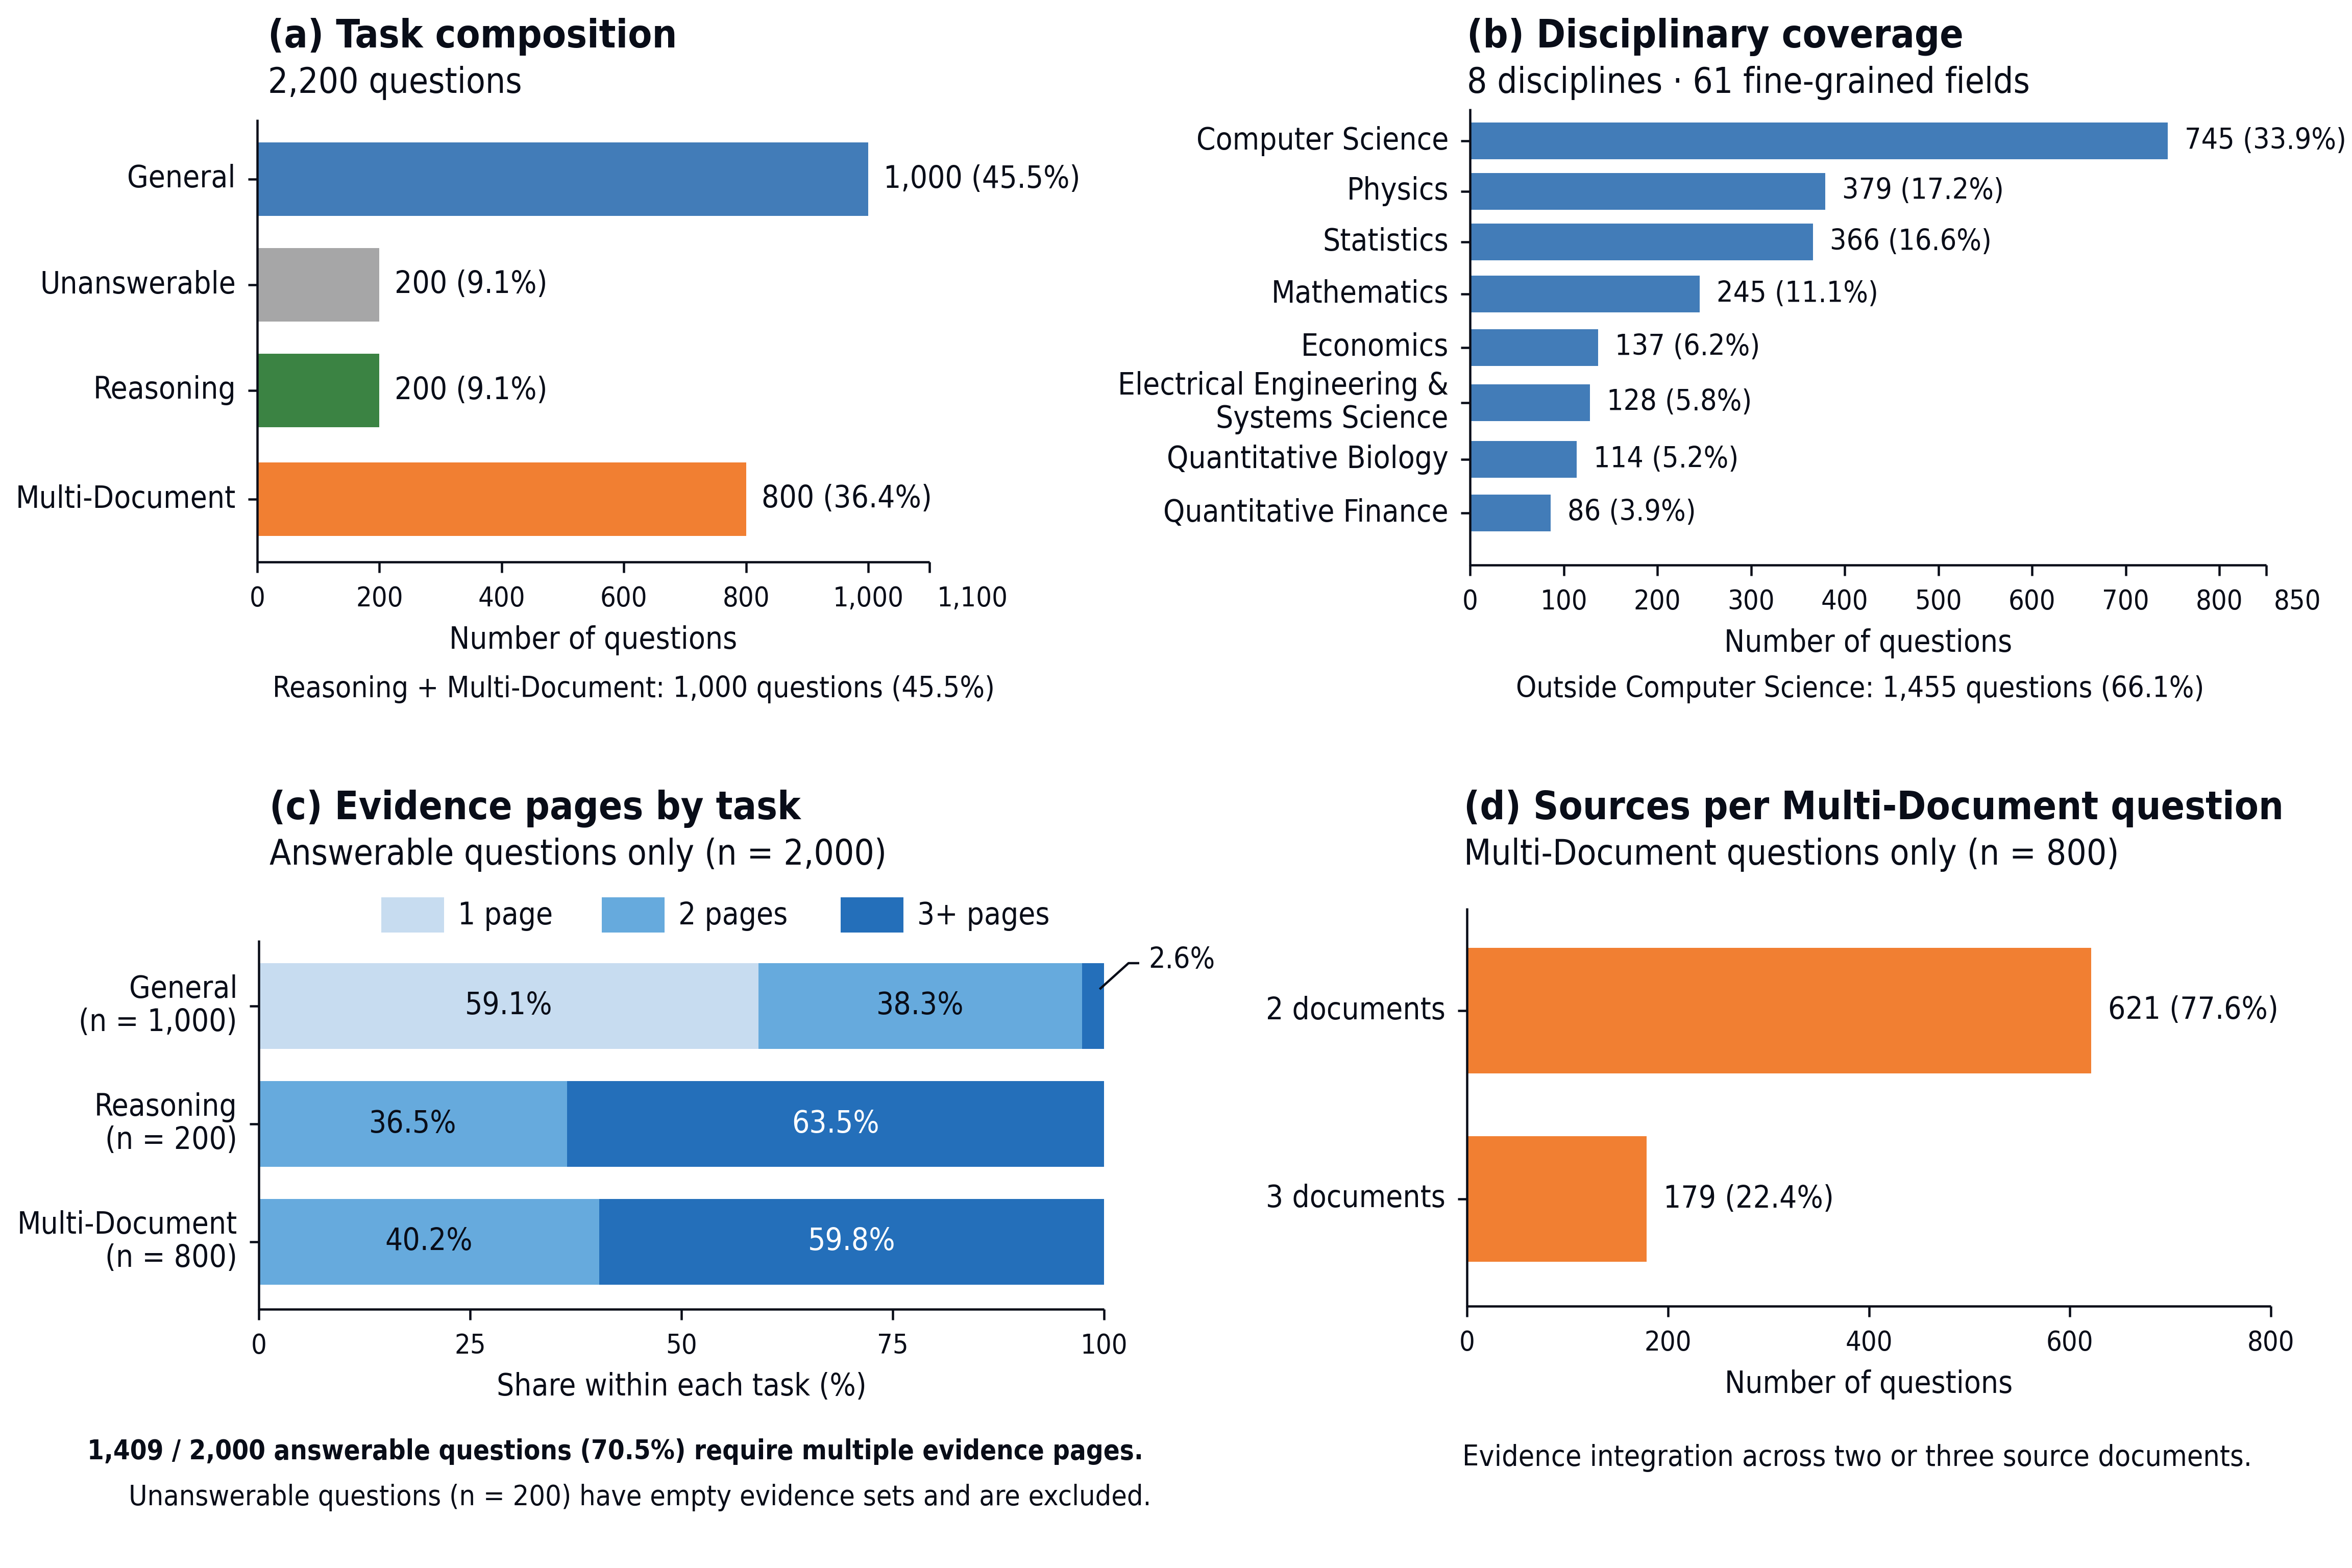
\includegraphics[width=\linewidth]{figures/fig_3_4_dataset_statistics.png}
    \caption{Dataset statistics of ScienceDoc. (a) Question counts by task. (b) Question counts by primary discipline. (c) Annotated evidence-page counts within each answerable task, normalized by its own sample size; the 200 Unanswerable questions have empty evidence sets and are excluded. (d) Number of source documents required per Multi-Document question. Percentages in (a) and (b) use all 2,200 questions, while (d) uses the 800 Multi-Document questions.}
    \label{fig:app_dataset_statistics}
\end{figure}

Panel (c) normalizes each evidence-page distribution by its task size: 1,000 General, 200 Reasoning, and 800 Multi-Document questions. General questions have one, two, or at least three evidence pages in 591, 383, and 26 cases, respectively. Reasoning questions have two pages in 73 cases and at least three in 127; the corresponding Multi-Document counts are 322 and 478. Thus, 1,409 of the 2,000 answerable questions (70.5\%) require multiple evidence pages. The same 1,409 questions represent 64.0\% of all 2,200 questions in Figure~\ref{fig:dataset_composition}; the difference is solely the denominator. The 200 Unanswerable questions have empty evidence sets and are excluded from panel (c).

Panel (d) uses the 800 Multi-Document questions as its denominator: 621 require two source documents and 179 require three. Source-document counts and evidence-page counts measure different aspects of the task, since each source may contribute multiple evidence pages. This distinction explains why the evidence-page and source-count distributions need not coincide.

\FloatBarrier

\subsection{Construction Lineage}
\label{app:construction_lineage}

The released benchmark is the result of a larger construction pool rather than a random sample of the initial questions. Document acquisition initially produced 6,204 candidate QA pairs from 703 documents. Format normalization, duplicate removal, page-range validation, and evidence review produced a 4,211-item single-document baseline over the retained 693-document corpus. This baseline supplied verified facts for subsequent General, unanswerable, and Reasoning construction, while additional grouping and source-necessity checks produced Multi-Document candidates. These historical counts describe intermediate pools only; they are not evaluation splits and are not used as denominators in the reported experiments.

Source-document counts and evaluation-PDF counts use different units: a merged PDF is an evaluation container, not an additional scientific document. The 693-document total in Section~\ref{sec:dataset} counts source documents, not merged evaluation containers.

\subsection{PDF and Page Representation}
\label{app:page_representation}

Source PDFs preserve their original text, equations, tables, figures, and layout. Related document-VQA benchmarks have likewise emphasized visual document
understanding across heterogeneous layouts and multiple document pages or
images~\cite{mathew2022infographicvqa,tanaka2023slidevqa}.For Multi-Document items, two or three source PDFs are concatenated in a fixed order without changing the content of their pages. The construction ledger records the source-document identifier, source-document order, source page, and corresponding merged page. Gold and predicted evidence always use PDF page indices in the evaluation PDF; printed page numbers in headers, footers, or the document body are never used as evidence indices.

Each evaluation record contains a question, concise reference answer,  annotated evidence pages, required evidence modalities, task type, question type, and answer format. Reasoning records additionally retain the source facts and their inferential relation. Multi-Document records retain the source-document map and the contribution required from each document. These audit fields support construction and review; the model-facing task remains the question plus PDF pages and the structured answer contract specified in Section~\ref{app:inference_protocol}.

\subsection{Construction Records and Evaluation Inputs}
\label{app:construction_records}

Intermediate generation batches, the single-document baseline, closed-book diagnostics, and candidate-review outputs are construction records. Evaluation uses only the four reviewed components described in the main text. Their release-file identities and freeze checks are specified in Section~\ref{app:final_freeze}.
\FloatBarrier
% END DATASET IMPORT 2026-09-12

% BEGIN APPENDIX IMPORT FROM Chinese draft 2026-09-15
\begingroup
\raggedbottom

The following construction details expand the expert-led workflow in Section~\ref{sec:dataset}. Human--model interaction has also been explored as a mechanism for constructing
and refining challenging benchmark instances~\cite{kiela2021dynabench}. Quality control and release checks are collected in Appendix~\ref{app:quality_control}, evaluation and reproduction in Appendix~\ref{app:detailed_protocol}, and qualitative analysis in Appendix~\ref{app:qualitative_analysis}.

\subsection{Construction Stages and Quality Gates}
\label{app:construction_pipeline}

Table~\ref{tab:app_stages} expands the construction overview in Figure~\ref{fig:dataset_pipeline} into operational stages. Each stage records input identities, processing dates, retained and rejected counts, model settings where applicable, and reasons for returning an item to revision.

\begin{table*}[!htb]
\centering
\caption{Construction stages, outputs, and quality gates.}
\label{tab:app_stages}
\footnotesize
\setlength{\tabcolsep}{3pt}
\renewcommand{\arraystretch}{1.15}
% Keep the font at its declared size; wrap columns instead of scaling the table.
\begin{tabularx}{\textwidth}{@{}
>{\hsize=.65\hsize\linewidth=\hsize\raggedright\arraybackslash}X
>{\hsize=.80\hsize\linewidth=\hsize\raggedright\arraybackslash}X
>{\hsize=1.10\hsize\linewidth=\hsize\raggedright\arraybackslash}X
>{\hsize=1.25\hsize\linewidth=\hsize\raggedright\arraybackslash}X
>{\hsize=1.20\hsize\linewidth=\hsize\raggedright\arraybackslash}X@{}}
\toprule
\textbf{Stage} & \textbf{Input} & \textbf{Executor / model} & \textbf{Key output} & \textbf{Condition for next stage} \\
\midrule
1. Document retrieval & Open-access platform categories and date ranges & Program + manual review & Document metadata and download list & Domain quotas, duplication checks, and licensing checks pass \\
2. PDF audit & Downloaded PDFs & PyMuPDF + manual review & Page count, file consistency, anomalous pages & File opens successfully and page indexing is stable \\
3. Basic QA & Single-document PDFs & Domain experts & Expert-written initial questions, answer requirements, and candidate evidence & Fields complete and evidence exists \\
4. Short-answer conversion & Mixed-format QA & Rules + manual review & Short-answer QA & No answer-choice leakage \\
5. Unanswerable & Document topic and missing facts & Domain experts + model-assisted rewriting + full-document review & Exact-refusal items & No sufficient evidence anywhere in the full document \\
6. Reasoning & Expert-designed question and verified QA from the same document & Domain experts + large language model assistance & Candidates combining necessary facts from 2--4 verified QA items & Every selected fact is indispensable; no conclusion leakage or stable question-only shortcut \\
7. Multi-Document & Expert-designed question and document groups & Domain experts + model-assisted expansion & Two-/three-document candidates & Every source is indispensable \\
8. Model-assisted dual review & Candidates + full PDFs & Two independent large language models & Dual-pass result or return reasons (dual KEEP means both independent reviewer models judge the item retainable) & Proceeds to human annotation and cross-validation, not direct release \\
9. Evidence recovery & Passed candidates + PDFs & Program + model + manual review & page and fact-level ledger & Page indices, sources, and modalities are consistent \\
10. Human final review & Final candidates & 10 annotators; at least two human experts independently verify each item & Keep, modify, delete, and cross-validation records & Every assigned item is closed out \\
11. Freeze and evaluate & Four official JSON files + PDFs & 11 MLLM runs + large language model Judge + fixed-denominator reporting & Per-item outputs for 11 models, answer and evidence-page metrics, strict reports, and exception records & Final 2,200 QA and PDFs pass preflight; missing predictions remain in the denominator; Judge and input identities are traceable \\
\bottomrule
\end{tabularx}
\end{table*}

A candidate advances only after passing its stage-specific gate; a returned item may be revised or deleted. Structural checks validate required fields,  page bounds, source identifiers, and duplicates keyed by both normalized question text and document identity. The resulting ledger separates candidate generation from human gold annotation: model-proposed answers and pages are review inputs, and evaluation outputs never redefine the reference answer.

\subsection{Document Retrieval, PDF Organization, and Basic QA}
\label{app:paper_retrieval}

The retrieval ledger stores the title, abstract, open-access platform category, assigned domain, filename, download status, and  page count. Category quotas guide acquisition; insufficient coverage can trigger a wider date range while retaining deduplication and readability checks. Table~\ref{tab:app_basic_checks} specifies the checks applied before semantic review. Field and page representations follow Section~\ref{app:dataset_details}.

\begin{table}[!htb]
\centering
\caption{Structural and content checks for documents and basic QA.}
\label{tab:app_basic_checks}
\small
\begin{tabularx}{\linewidth}{l X X}
\toprule
\textbf{Object} & \textbf{Check} & \textbf{Failure handling} \\
\midrule
File & Openability, page count, duplicate files & Add to exception list; exclude from question construction \\
Question & Complete, unambiguous, no answer leakage & Rewrite or delete \\
Answer & Facts, units, precision, direction & Return to the PDF and correct \\
Evidence pages & Pages, direct support, minimally sufficient & Add missing pages, remove redundant pages, or delete the item \\
Modality & \texttt{text/figure/table/equation} & Relabel according to the actual evidence \\
\bottomrule
\end{tabularx}
\end{table}

Modality labels describe evidence needed for the answer: \texttt{text} alone is used when textual evidence is sufficient, while \texttt{equation}, \texttt{table}, or \texttt{figure} is added only when that modality is required. Reviewers remove background-only pages and retain a minimally sufficient set of direct supporting pages.

\subsection{Construction of Unanswerable Questions}
\label{app:unanswerable_construction}

Following prior work on unanswerable QA~\cite{rajpurkar2018know}, experts anchor each candidate in a method, variable, dataset, or experimental setting explicitly present in the document, then identify a specific missing relation or value. The queried relation must connect to the research objective; absent personal details or unrelated facts are rejected as off-topic. Model assistance is limited to rewriting or proposing variants of this expert-defined information need.

The generation model receives the expert-designed question and missing-information requirement, together with the title, abstract, section headings, entity list, and summaries of verified answerable QA. Its output must include a nonempty question, identifiable \texttt{anchored\_\allowbreak entities}, a concrete \texttt{missing\_\allowbreak evidence} description, and an auditable rationale. These fields describe a candidate, not a gold answer. The complete prompt used for expert-guided unanswerable candidate generation is shown in Figure~\ref{fig:app_unanswerable_generation_prompt}.

For retained items, the reference answer is exactly \texttt{Unanswerable} and \texttt{evidence\_\allowbreak pages} is \texttt{[]}. Under PDF inference, a refusal with a nonempty page list violates the output contract. The exact label provides a consistent representation of the evidence-insufficiency decision described in the main text.


% BEGIN APPENDIX PROMPT 01_unanswerable_generation
\par\smallskip
\noindent\begin{minipage}{\linewidth}
    \centering
    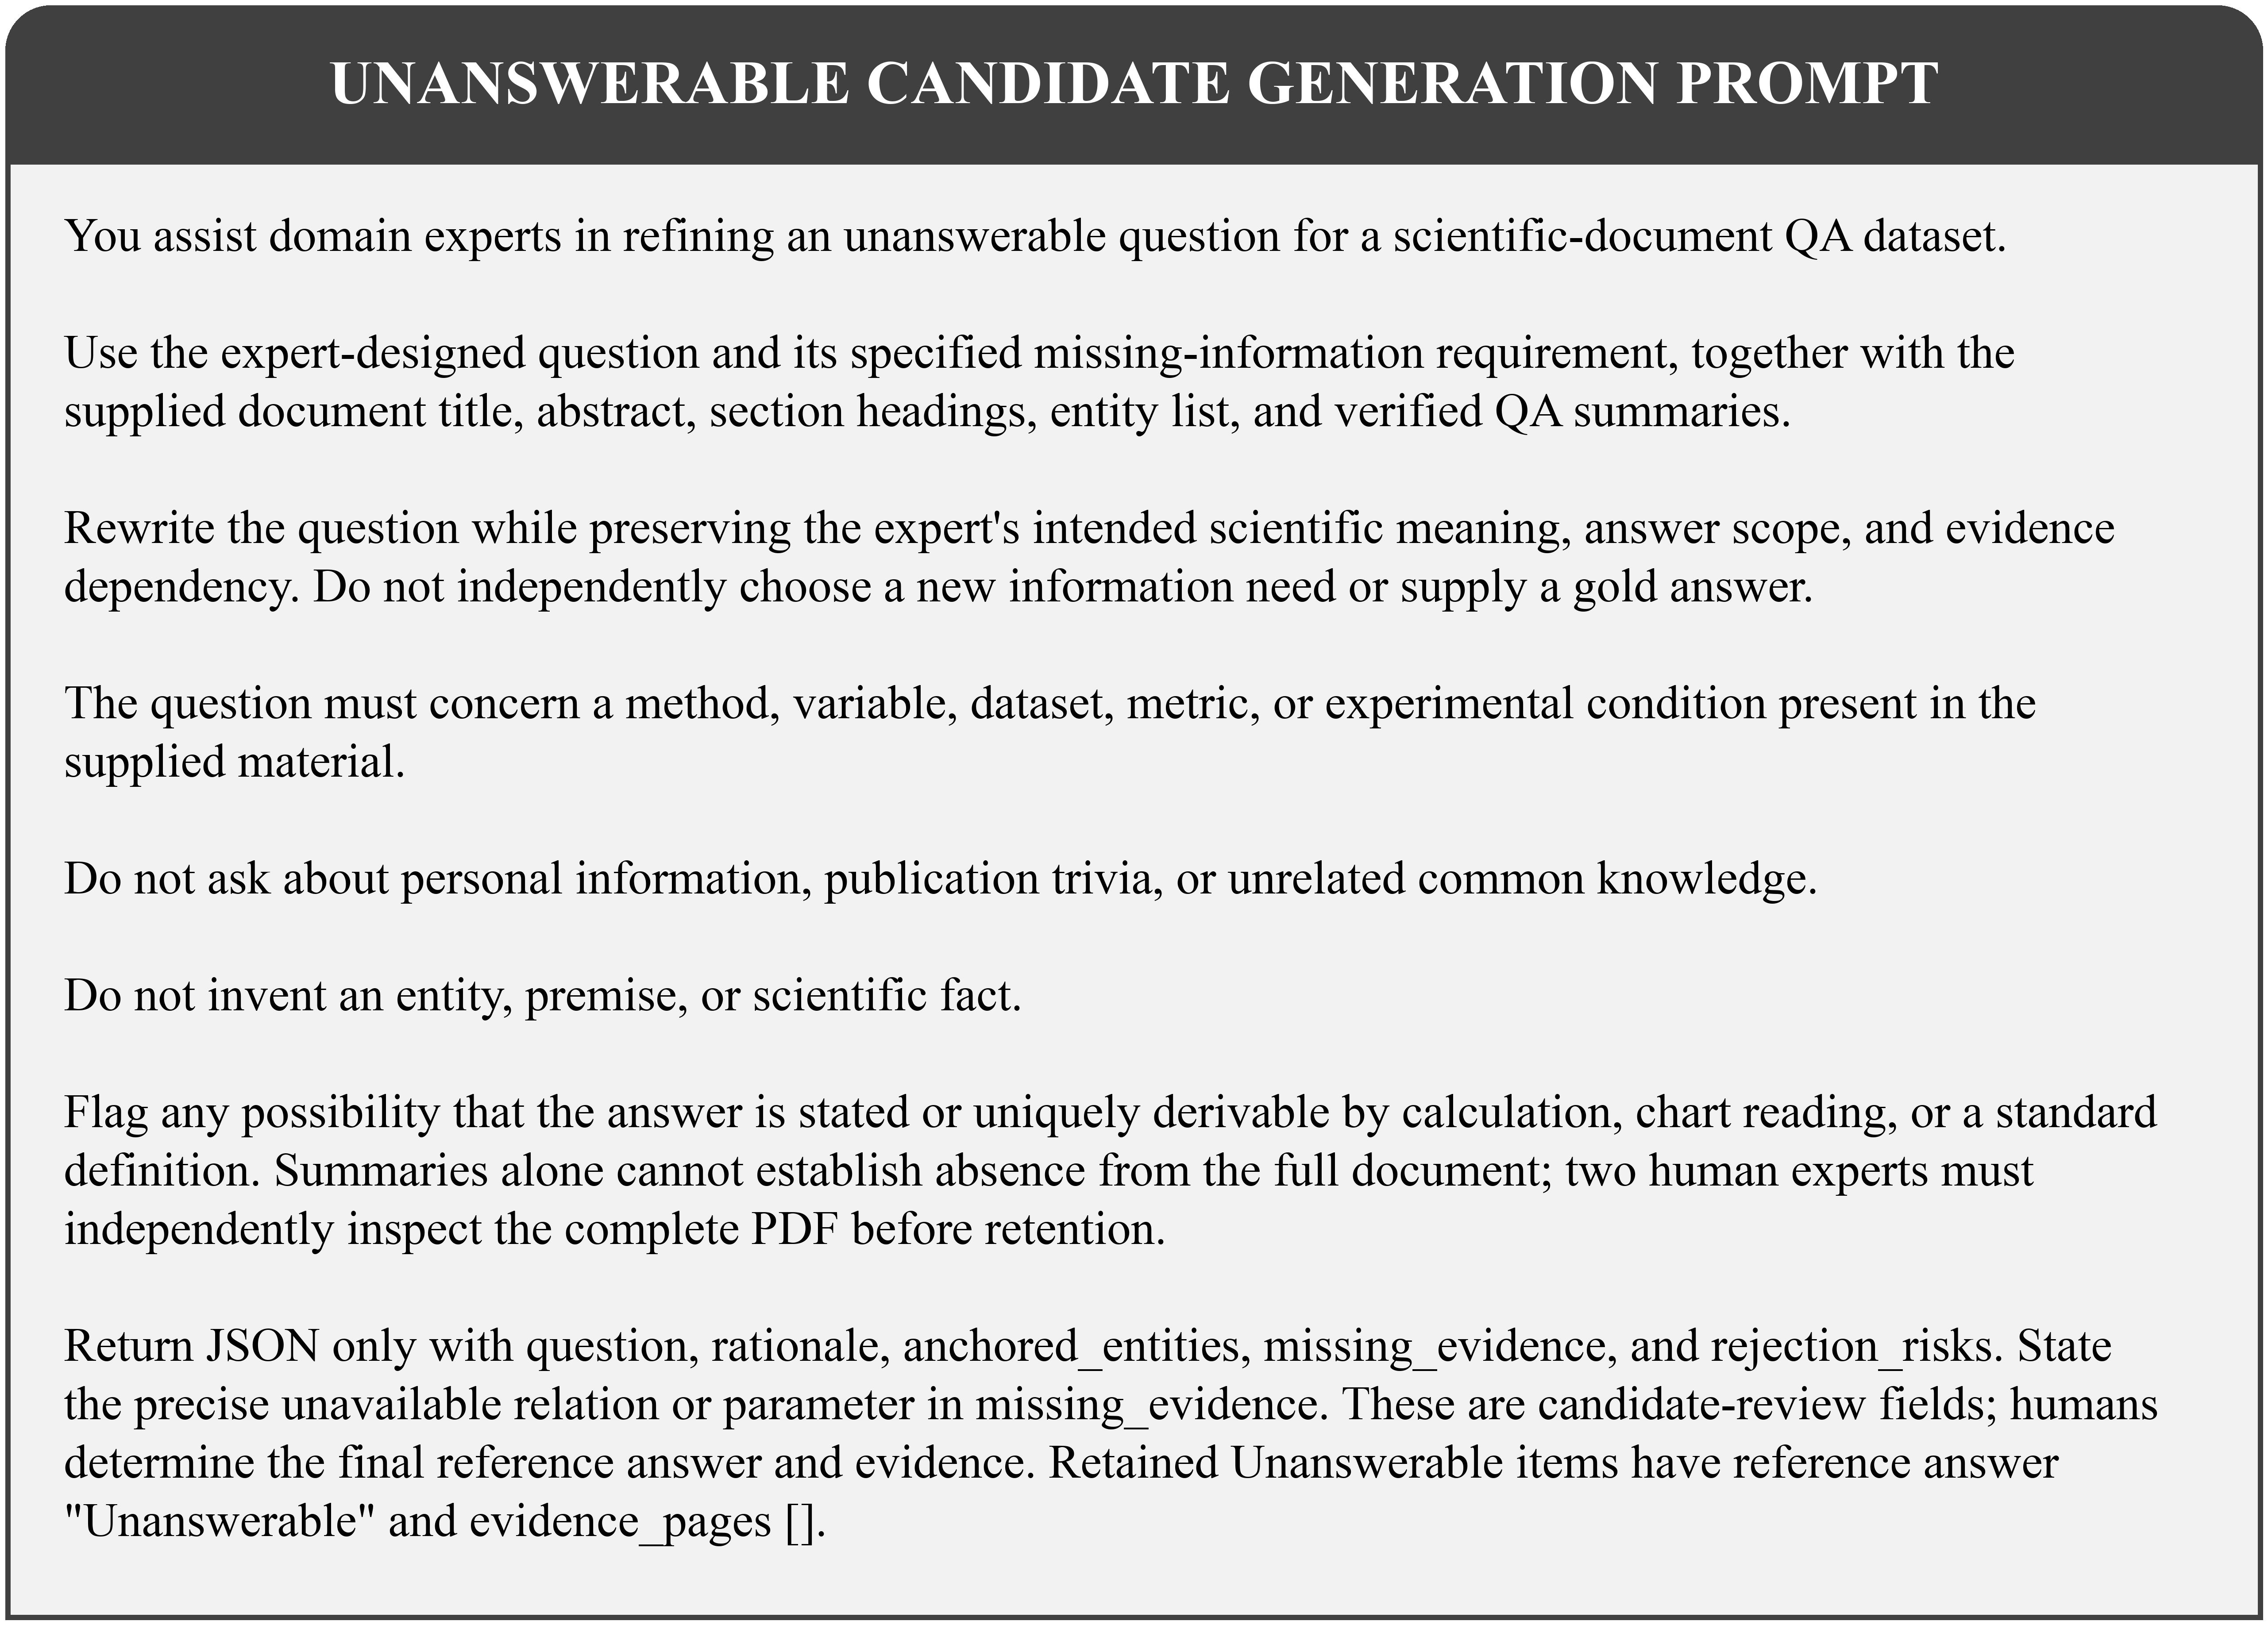
\includegraphics[width=0.88\linewidth]{figures/appendix_prompt_01_unanswerable_generation.png}
    \captionsetup{font=small,skip=3pt}
    \captionof{figure}{Prompt for expert-guided generation of unanswerable-question candidates.}
    \label{fig:app_unanswerable_generation_prompt}
\end{minipage}
\par\smallskip
% END APPENDIX PROMPT 01_unanswerable_generation


Two human reviewers independently check the entire supplied PDF, including appendices, captions, footnotes, and any included supplementary pages. Each records the topic anchor, searched locations, missing fact, and a nearby statement that does not close the gap. A candidate is rejected as unanswerable if a value can be read reliably from a plot or derived uniquely from the stated parameters, even when the answer is not written verbatim. Disagreement requires renewed inspection of specific pages. Closed-book screening (Section~\ref{app:reasoning_filtering}) can additionally reveal question cues or common-knowledge shortcuts; its outputs are retained only as construction diagnostics.

\subsection{Single-Document Reasoning Candidate Generation}
\label{app:reasoning_generation}

Experts specify the intended reasoning relation and necessary facts from 2--4 verified QA records belonging to the same document. Related multi-hop QA benchmarks similarly emphasize compositional reasoning over
multiple supporting facts and explicit reasoning dependencies
~\cite{yang2018hotpotqa,ho2020wikimultihop}. A large language model receives the expert-designed question, required reasoning relation, verified source questions and answers, and document identity, without PDF pages or evidence indices, and proposes a candidate formulation. Supported relation labels are \texttt{causal\_\allowbreak chain}, \texttt{conditional\_\allowbreak inference}, \texttt{comparison}, \texttt{constraint\_\allowbreak intersection}, and \texttt{multi\_\allowbreak step\_\allowbreak calculation}.

Candidate records contain \texttt{reasoning\_\allowbreak type}, \texttt{intermediate\_\allowbreak facts}, a proposed \texttt{answer}, and \texttt{source\_\allowbreak qa\_\allowbreak ids}. Validation confirms that all source IDs exist, refer to the same document, and contribute necessary facts. The answer must follow through an explicit operation or relation rather than concatenating source answers, and the new question must neither copy a source question nor reveal its conclusion. Human reviewers subsequently determine the reference answer and evidence from the PDF. The prompt used for reasoning-candidate generation is shown in Figure~\ref{fig:app_reasoning_generation_prompt}.

% BEGIN APPENDIX PROMPT 02_reasoning_generation
\par\medskip
\noindent\begin{minipage}{\linewidth}
\mbox{}\par\smallskip
    \centering
    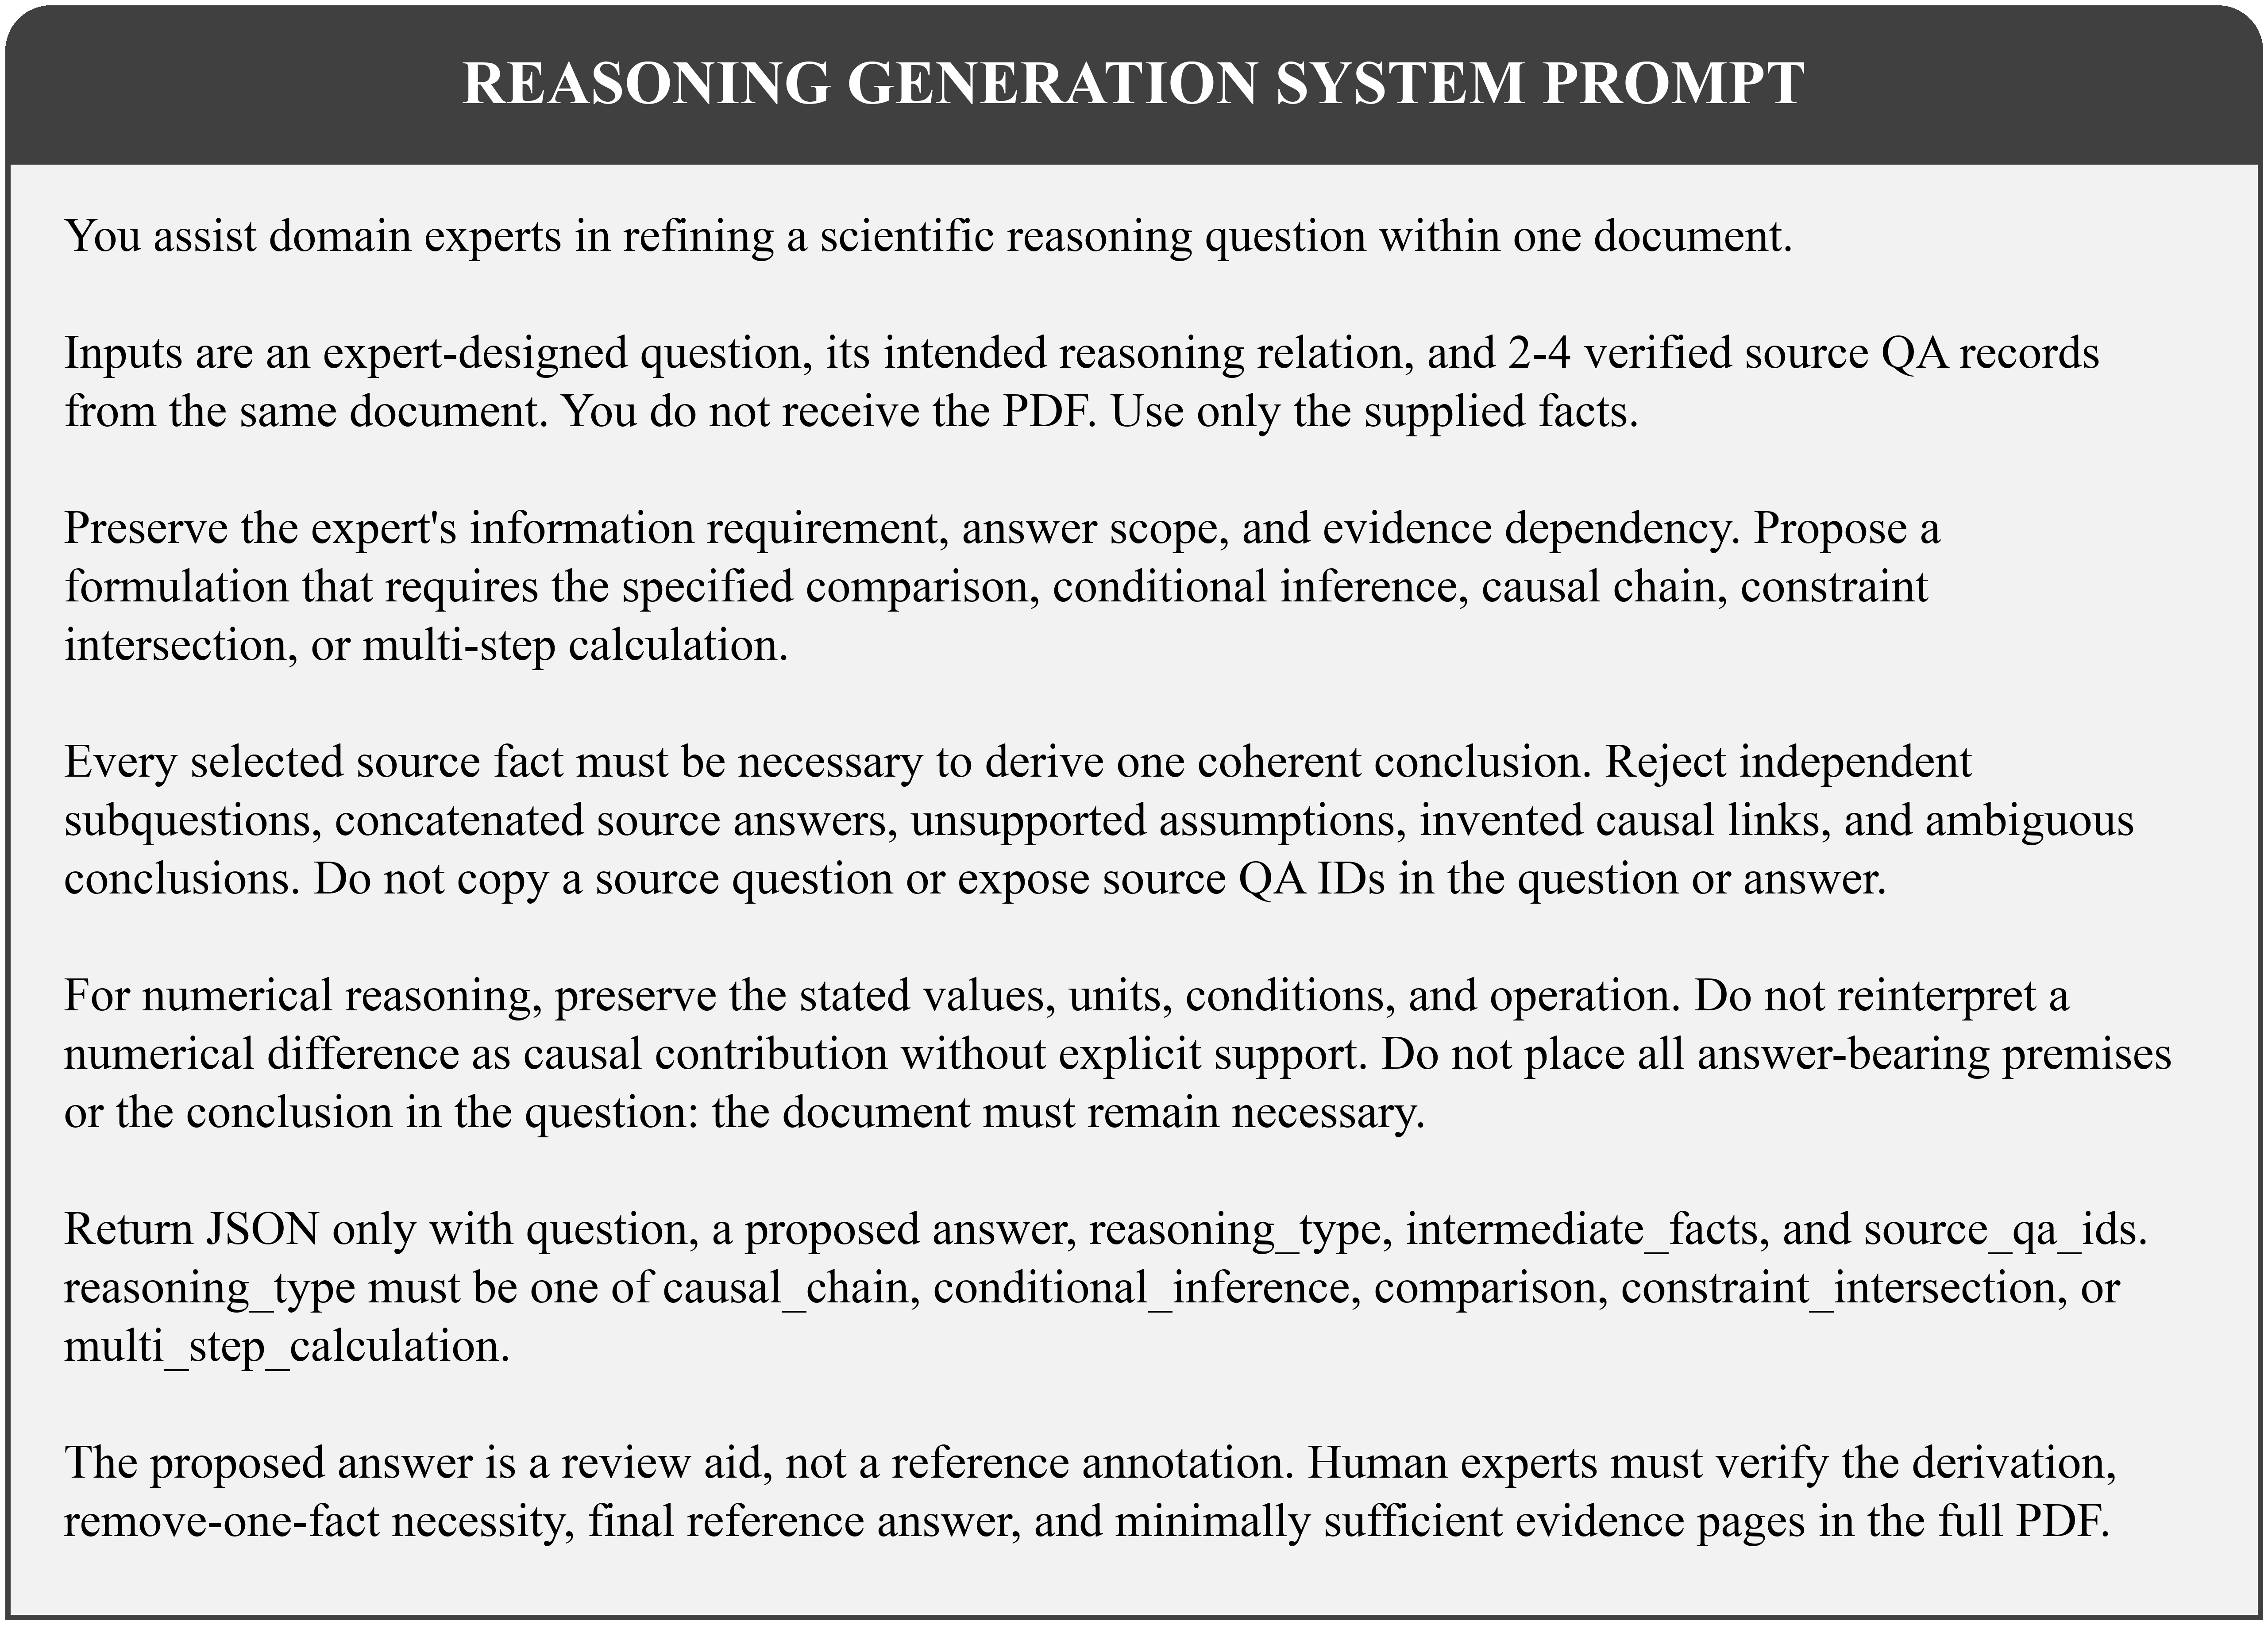
\includegraphics[width=0.96\linewidth]{figures/appendix_prompt_02_reasoning_generation.png}
    \captionof{figure}{Expert-guided prompt for reasoning-candidate generation.}
    \label{fig:app_reasoning_generation_prompt}
\end{minipage}\par\medskip
% END APPENDIX PROMPT 02_reasoning_generation

% BEGIN APPENDIX PROMPT 02_reasoning_generation
% \par\medskip
% \noindent\begin{minipage}{\linewidth}
% \paragraph{Expert-guided Reasoning candidate prompt.}\mbox{}\par\smallskip
%     \centering
%     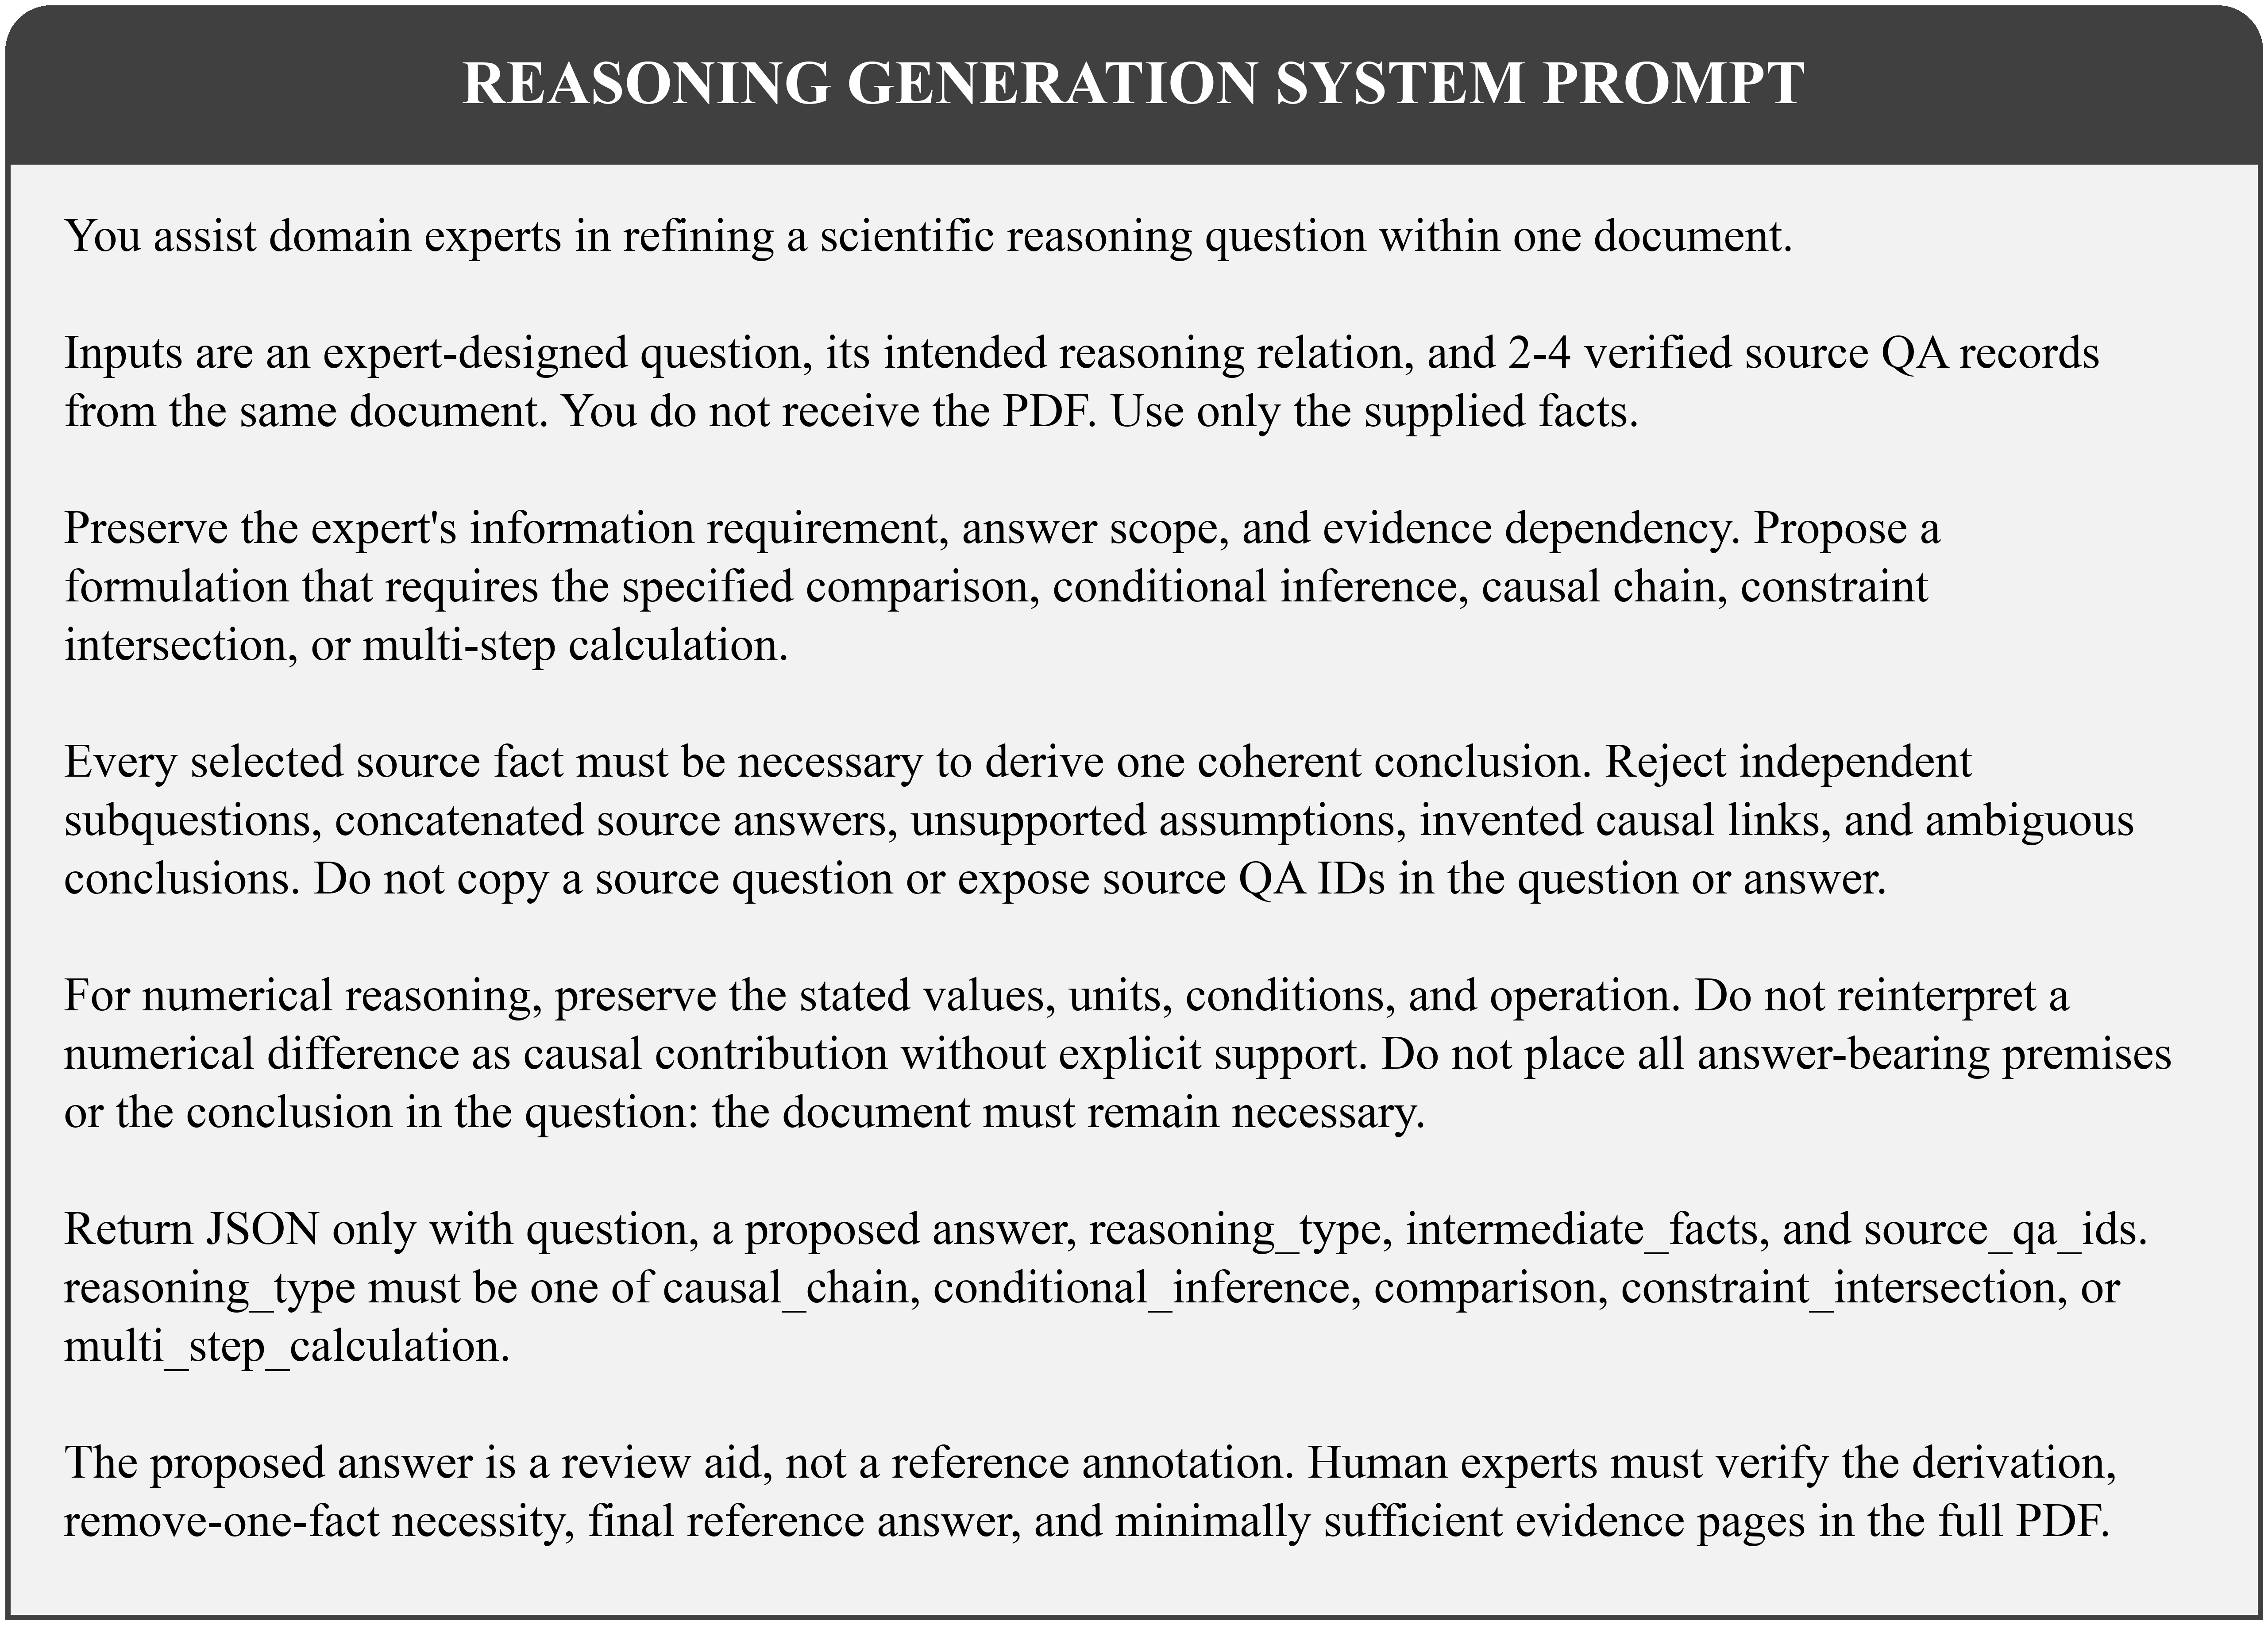
\includegraphics[width=0.96\linewidth]{figures/appendix_prompt_02_reasoning_generation.png}
% \end{minipage}\par\medskip
% END APPENDIX PROMPT 02_reasoning_generation

\subsection{Reasoning Difficulty Filtering and Closed-Book Ablation}
\label{app:reasoning_filtering}

Filtering checks source identity, answer leakage, and completeness of the derivation. Reviewers decompose a candidate into premises, operations, and conclusion, rejecting unstated assumptions or multiple possible answers. Per-hop ablation removes one required fact at a time and checks whether the complete conclusion still follows. Evidence recovery checks page support for each remaining step. As reported in Section~\ref{sec:dataset}, all retained Reasoning questions require evidence from multiple pages; no additional minimum distance between these pages is imposed.

The \texttt{question\_\allowbreak only} diagnostic sends only the question to two large language models. Consistently correct closed-book answers flag possible question leakage, common knowledge, or insufficient document dependence and trigger revision or exclusion. Failure in this diagnostic alone does not establish difficulty under PDF input.The closed-book diagnostic prompt is shown in Figure~\ref{fig:app_closed_book_prompt}.

% BEGIN APPENDIX PROMPT 03_closed_book
\par\medskip
\noindent\begin{minipage}{\linewidth}
    \centering
    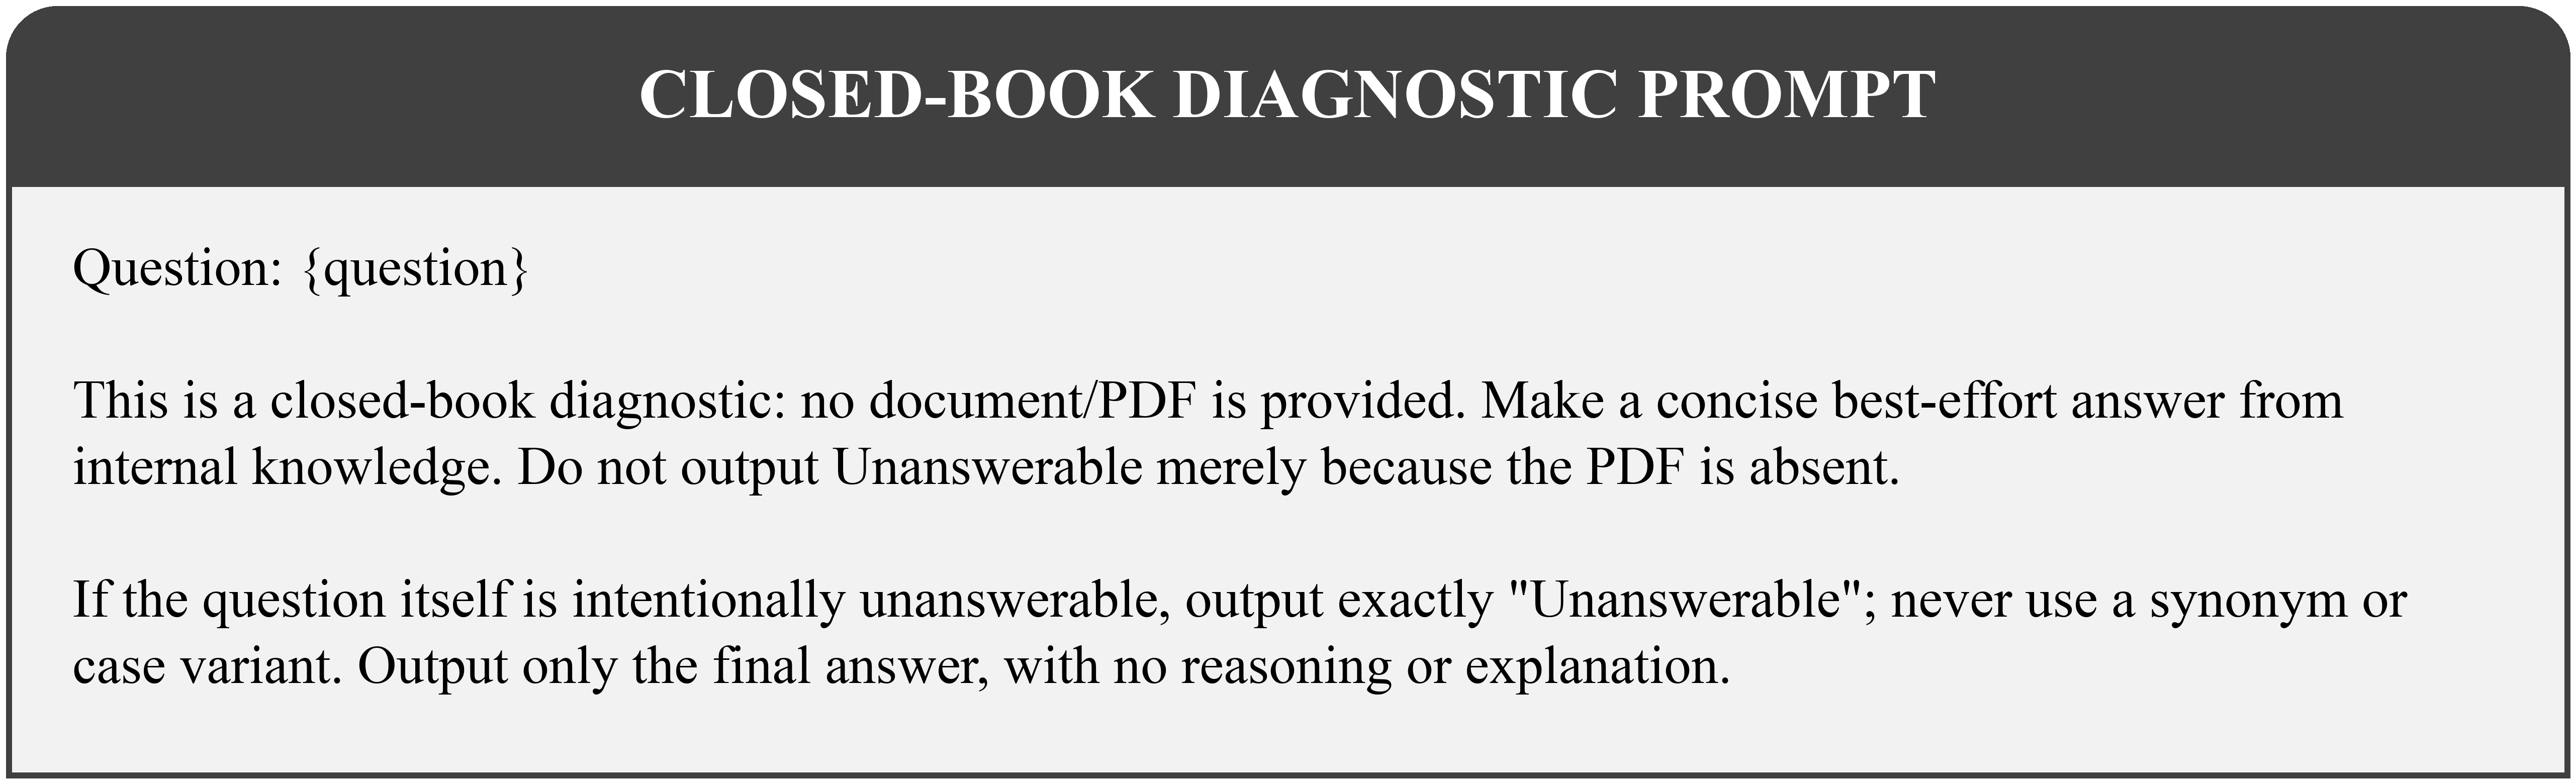
\includegraphics[width=0.96\linewidth]{figures/appendix_prompt_03_closed_book.png}
    \captionof{figure}{Prompt for the closed-book diagnostic.}
    \label{fig:app_closed_book_prompt}
\end{minipage}\par\medskip
% END APPENDIX PROMPT 03_closed_book

% BEGIN APPENDIX PROMPT 03_closed_book
% \par\medskip
% \noindent\begin{minipage}{\linewidth}
% \paragraph{Closed-book diagnostic prompt.}\mbox{}\par\smallskip
%     \centering
%     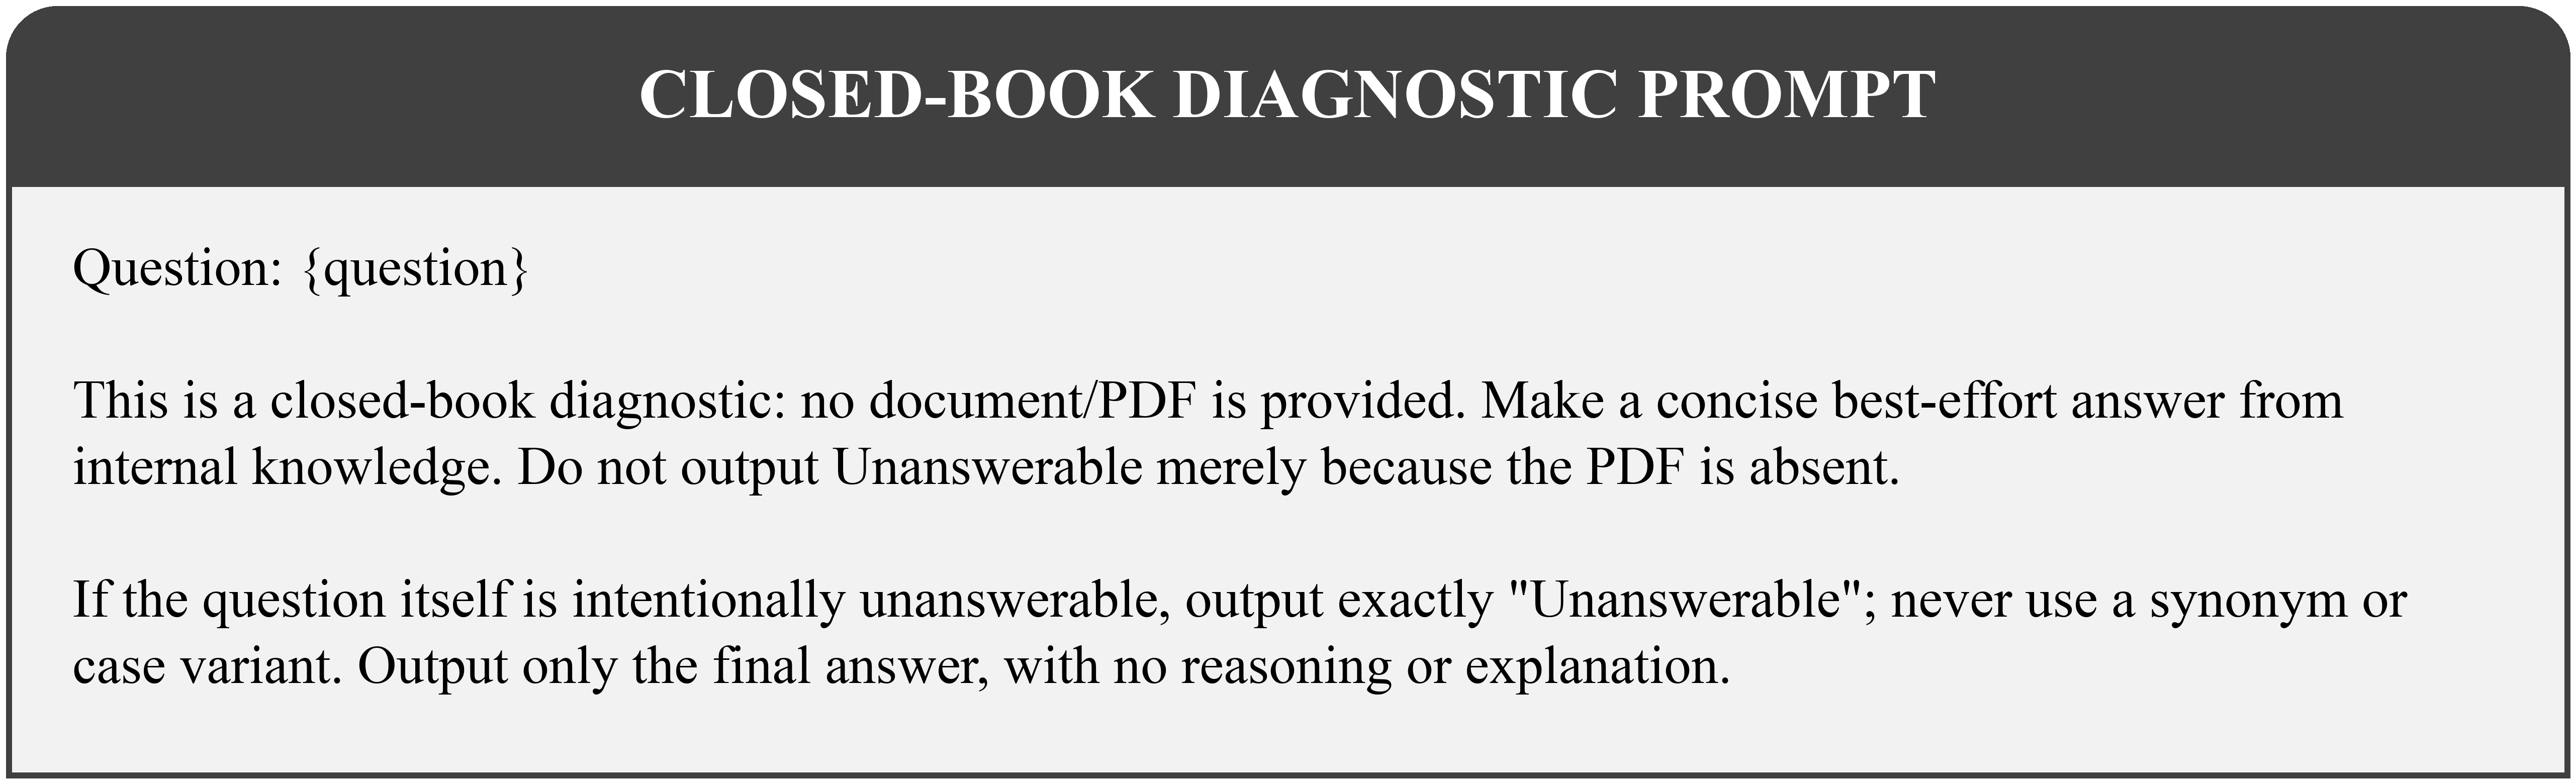
\includegraphics[width=0.96\linewidth]{figures/appendix_prompt_03_closed_book.png}
% \end{minipage}\par\medskip
% END APPENDIX PROMPT 03_closed_book

Closed-book outputs, screening decisions, and revision reasons remain in the construction ledger and are excluded from the main benchmark scores. The reported experiments use the PDF protocol; Full, Oracle, and evidence-page ablations are page-selection policies within that protocol, not additional tasks.

\subsection{Multi-Document Grouping, Generation, and Source Ablation}
\label{app:cross_pdf_generation}

Experts group two or three documents by disciplinary relevance and complementary evidence, then define the information required from each source. A relation ledger records source-document identifiers, document order, title keywords, each source's factual contribution, and the expected relation. Large language models use the expert-designed question, specified source contributions, verified QA text, and document titles to propose candidate formulations; full PDFs are reserved for review and evidence recovery.

Candidate relations include comparisons under a common metric, component compatibility, shared failure conditions, constraint intersections, methodological differences, and cross-study validation. Juxtaposed answers, generic shared background, and links requiring external knowledge are rejected.

For source ablation, reviewers remove each document in turn and record which part of the complete answer becomes unsupported. A three-document candidate must require all three documents; a question answerable from a subset is revised or discarded. The source-to-merged-page map defined in Section~\ref{app:dataset_details} is checked independently so that document order cannot introduce evidence-index errors.The prompt used for multi-document candidate generation is shown in Figure~\ref{fig:app_multi_document_generation_prompt}.

% BEGIN APPENDIX PROMPT 04_multi_document_generation
\par\medskip
\noindent\begin{minipage}{\linewidth}
    \centering
    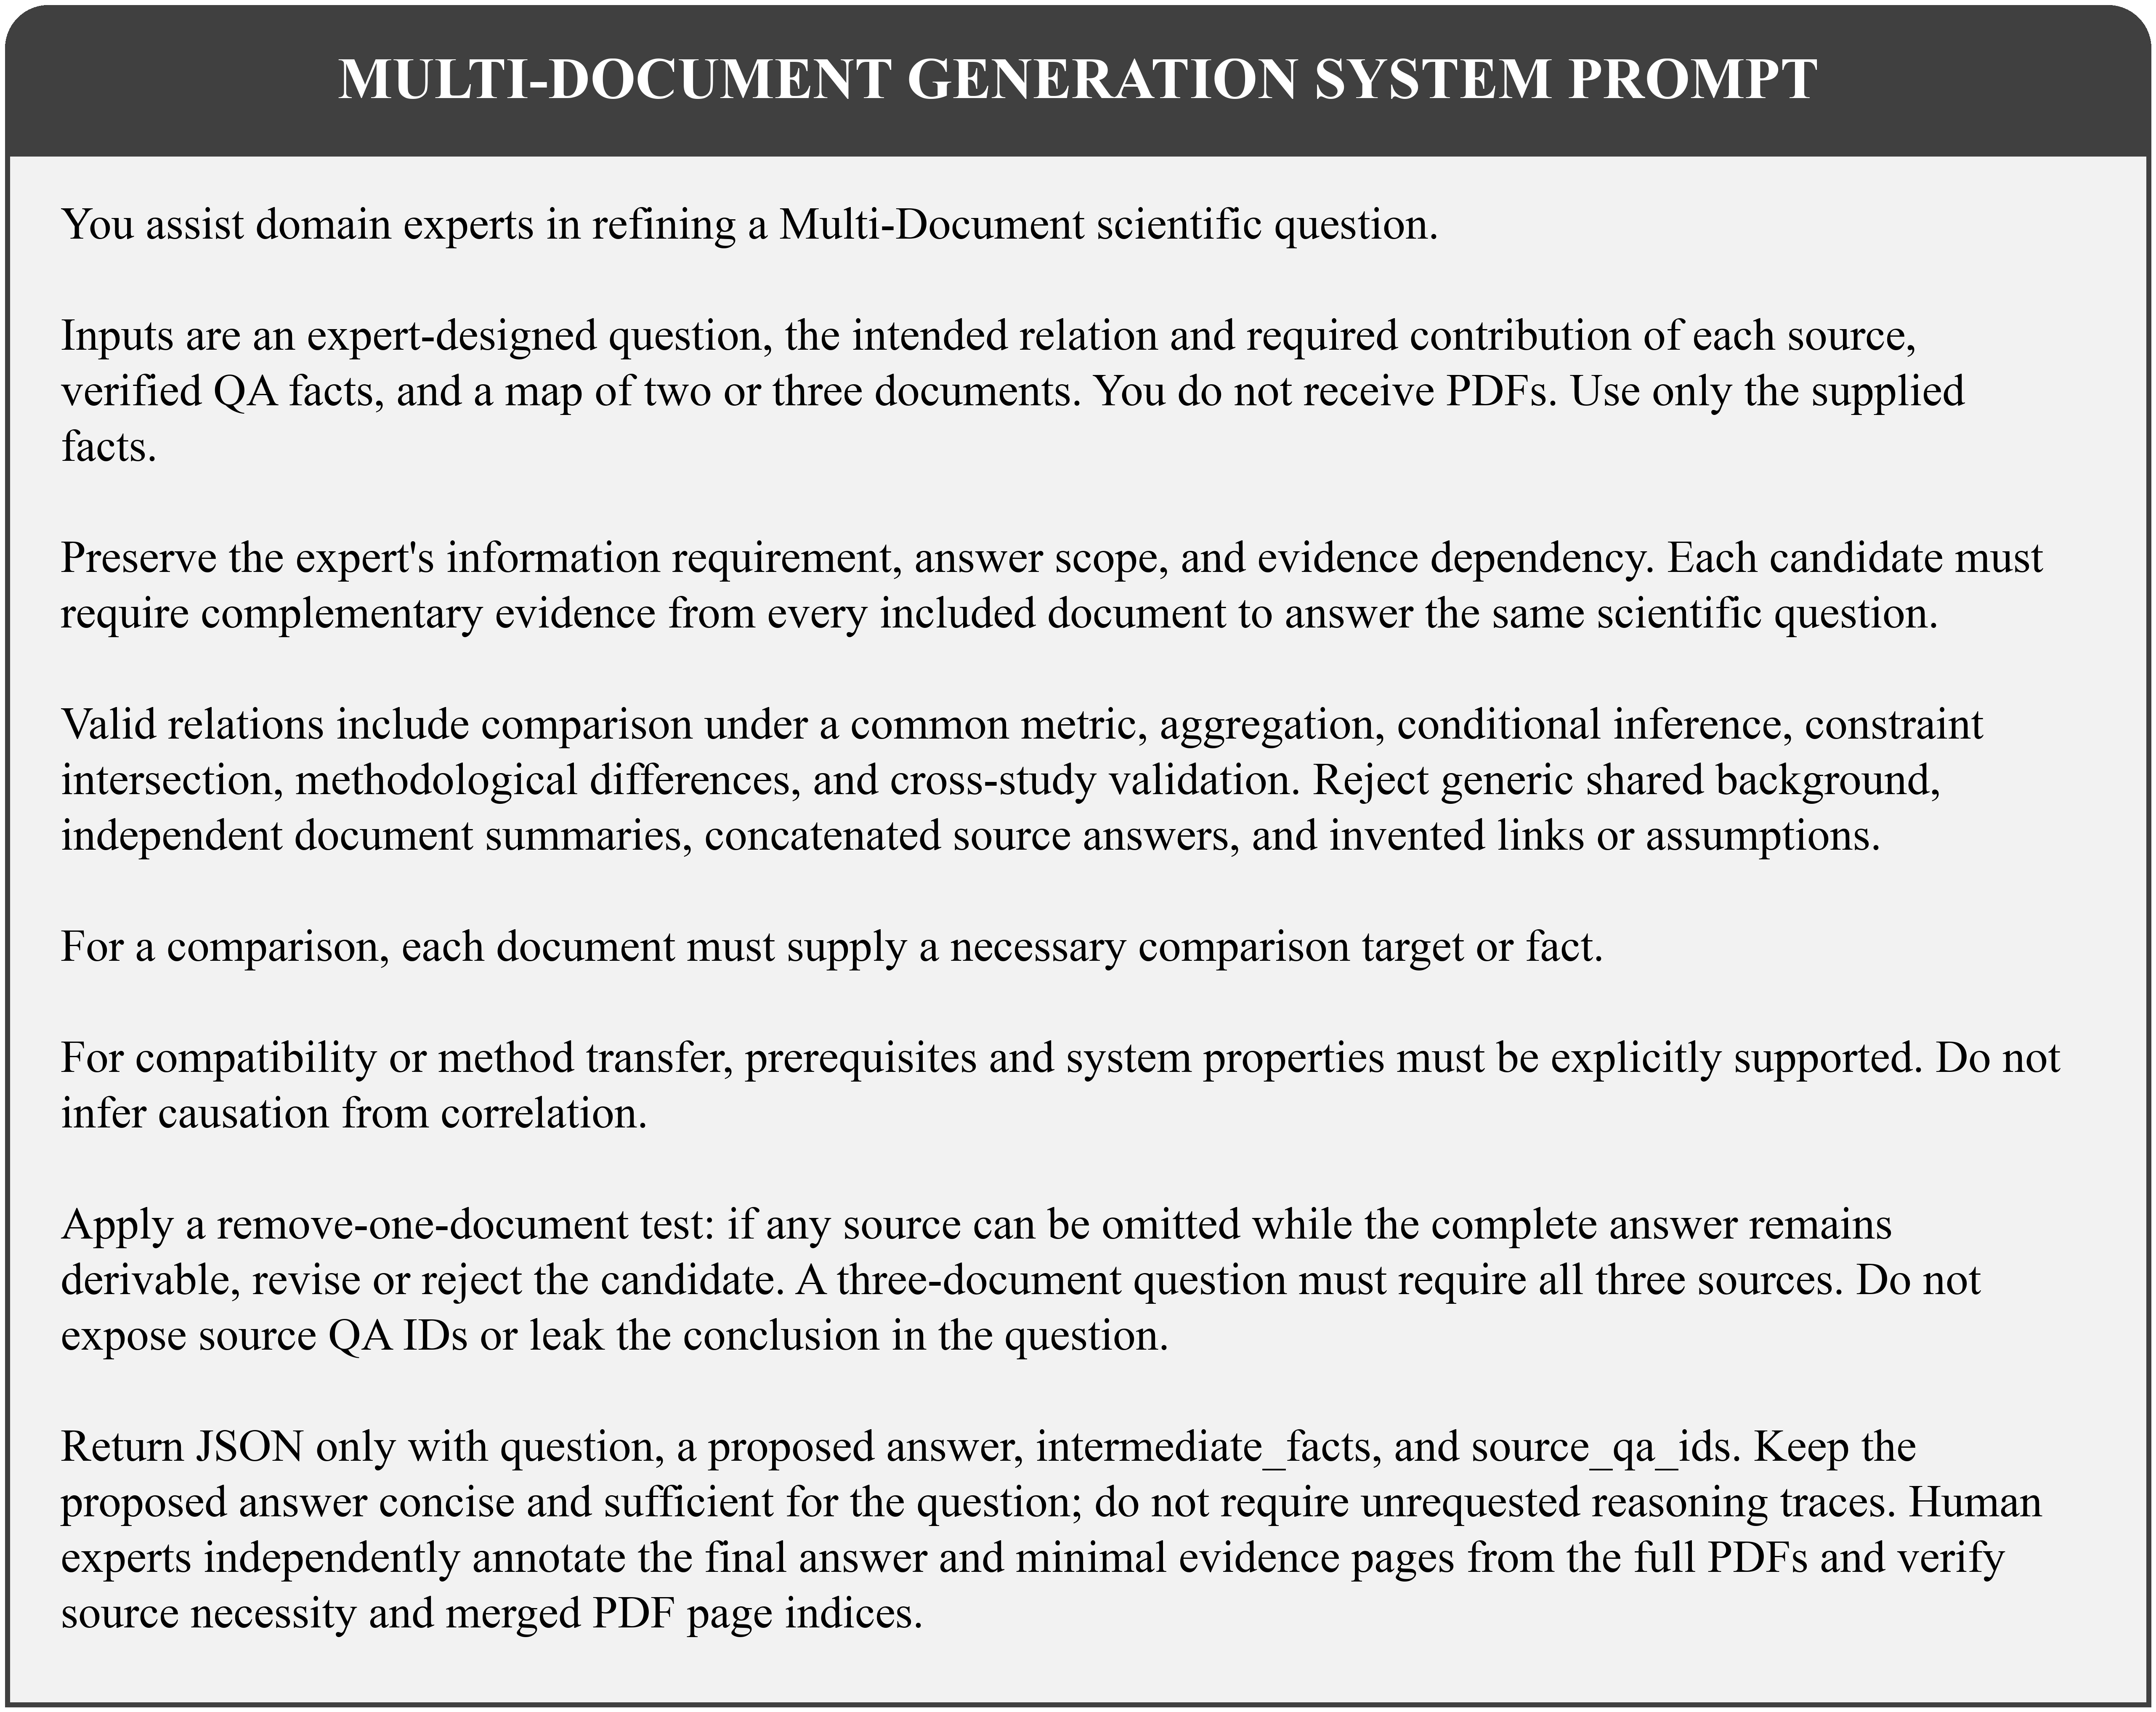
\includegraphics[width=0.96\linewidth]{figures/appendix_prompt_04_multi_document_generation.png}
    \captionof{figure}{Expert-guided prompt for multi-document candidate generation.}
    \label{fig:app_multi_document_generation_prompt}
\end{minipage}\par\medskip
% END APPENDIX PROMPT 04_multi_document_generation

% BEGIN APPENDIX PROMPT 04_multi_document_generation
% \par\medskip
% \noindent\begin{minipage}{\linewidth}
% \paragraph{Expert-guided Multi-Document candidate prompt.}\mbox{}\par\smallskip
%     \centering
%     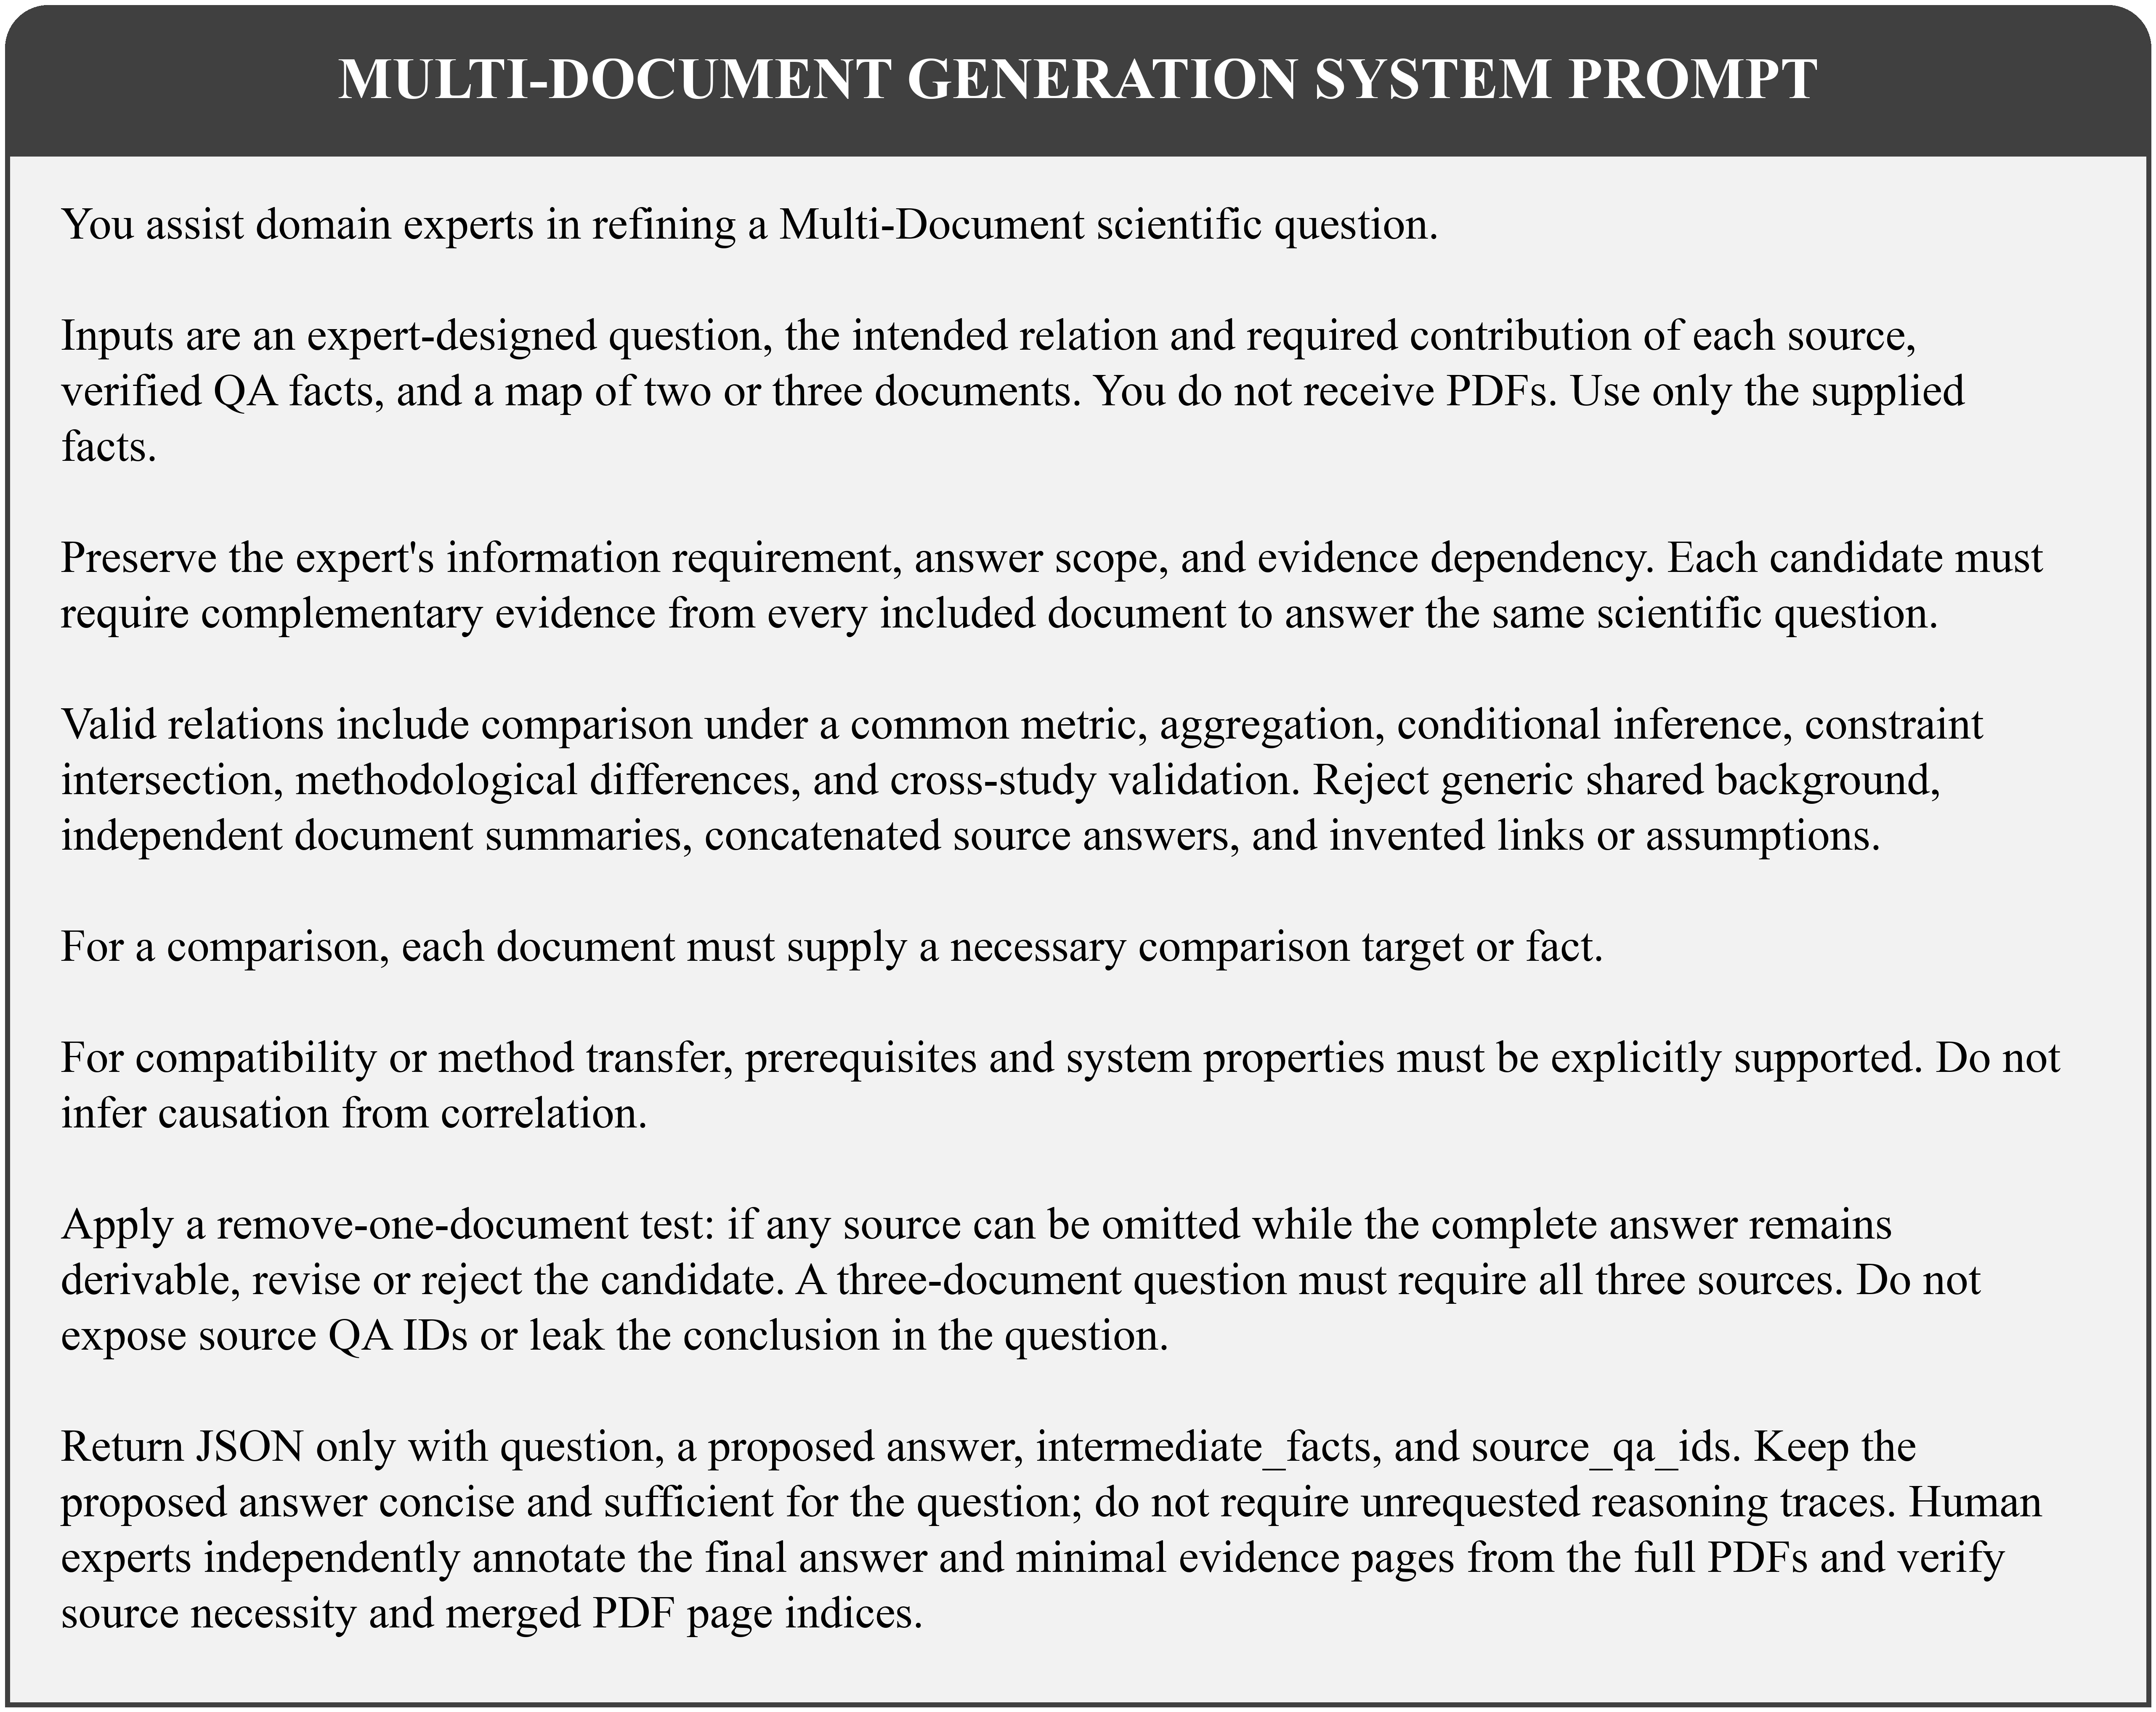
\includegraphics[width=0.96\linewidth]{figures/appendix_prompt_04_multi_document_generation.png}
% \end{minipage}\par\medskip
% END APPENDIX PROMPT 04_multi_document_generation

\FloatBarrier

\section{Quality Control and Dataset Release}
\label{app:quality_control}

This section details the review workflow and release checks supporting the professional annotation and independent human cross-validation described in Section~\ref{sec:dataset}.

\subsection{Model-Assisted Dual Review and Evidence Recovery}
\label{app:dual_review}

Two large language models independently receive the same question, proposed answer, and full PDF pages. They do not see one another's decisions. Each record contains \texttt{decision}, \texttt{confidence}, \texttt{reason}, model identity, and page-level \texttt{supported\_\allowbreak fact}.

Dual KEEP advances a candidate to evidence recovery. FIX requires revision and resubmission; REJECT routes the item to human inspection or deletion. This is a conjunctive filter, not a majority vote, and never bypasses the human cross-validation required in the main text. Table~\ref{tab:app_dual_review} lists the review dimensions.

Evidence recovery links each intermediate fact to its \texttt{ PDF\_\allowbreak PAGE}; Multi-Document records additionally store \texttt{source\_\allowbreak doc\_\allowbreak number} and \texttt{source\_\allowbreak page}. A modality audit then applies the evidence-necessity rule in Section~\ref{app:paper_retrieval}.

\begin{table}[!htb]
\centering
\caption{Independent model-assisted review checks and final gates.}
\label{tab:app_dual_review}
\small
\begin{tabularx}{\linewidth}{l X X X}
\toprule
\textbf{Review item} & \textbf{Large model 1} & \textbf{Large model 2} & \textbf{Final gate} \\
\midrule
Answer entailment & Independent full-document reading & Independent full-document reading & Both pass \\
Evidence completeness & Fact-level page indices & Fact-level page indices & No missing hop \\
Source necessity & Remove-document test & Remove-document test & Every included source is indispensable \\
Question leakage & Closed-book answerability & Question-cue check & No direct answer leakage \\
Modality & Visual evidence on pages & Visual evidence on pages & Human confirmation of canonical value \\
\bottomrule
\end{tabularx}
\end{table}


\subsection{Human Final Review and Front-End Validation}
\label{app:human_review}

The review interface implements the professional annotation and independent cross-validation described in the main text. Reviewers first confirm \texttt{dataset\_\allowbreak id}, document identity, and \texttt{qa\_\allowbreak id}, then inspect the question and fields alongside the corresponding PDF (Figure~\ref{fig:app_manual_review}).

Question checks cover entities, time ranges, comparison targets, direction, units, and output format. Answer checks cover numerical values, signs, percentages, abbreviations, names, and conditions. Evidence checks require reviewers to state, page by page, which fact in the answer is supported by that page; pages that provide only background but do not support the answer are removed. Reasoning items undergo per-hop ablation, whereas Multi-Document items undergo per-source ablation.


Reviewers can keep, modify, delete, or defer an item. Before modification or deletion, the system saves a complete snapshot; after write-back, it records the account, time, previous value, new value, and reason. If the underlying file changes during review, the reviewer must reopen and reassess it rather than overwriting another person's modifications.

\begin{table}[!htb]
\centering
\caption{Manual-review actions and audit records.}
\label{tab:app_human_actions}
\small
\begin{tabularx}{\linewidth}{l X X}
\toprule
\textbf{Action} & \textbf{When used} & \textbf{System record} \\
\midrule
Keep & Question, answer, evidence, and dependencies are all correct & Status and reviewer \\
Modify & The correct value can be determined uniquely from the PDF & Full pre-modification snapshot and updated value \\
Delete & The question is invalid or cannot be repaired reliably & Deletion tombstone and snapshot \\
Defer & PDF anomaly, multiple possible repairs, or unclear source & Remains incomplete and is escalated \\
\bottomrule
\end{tabularx}
\end{table}

The interface flags missing fields, out-of-range or duplicate page indices, and noncanonical labels. Semantic acceptance remains a human decision; every modification, deletion, or deferral requires a recorded reason.


\begin{figure}[!htb]
    \centering
    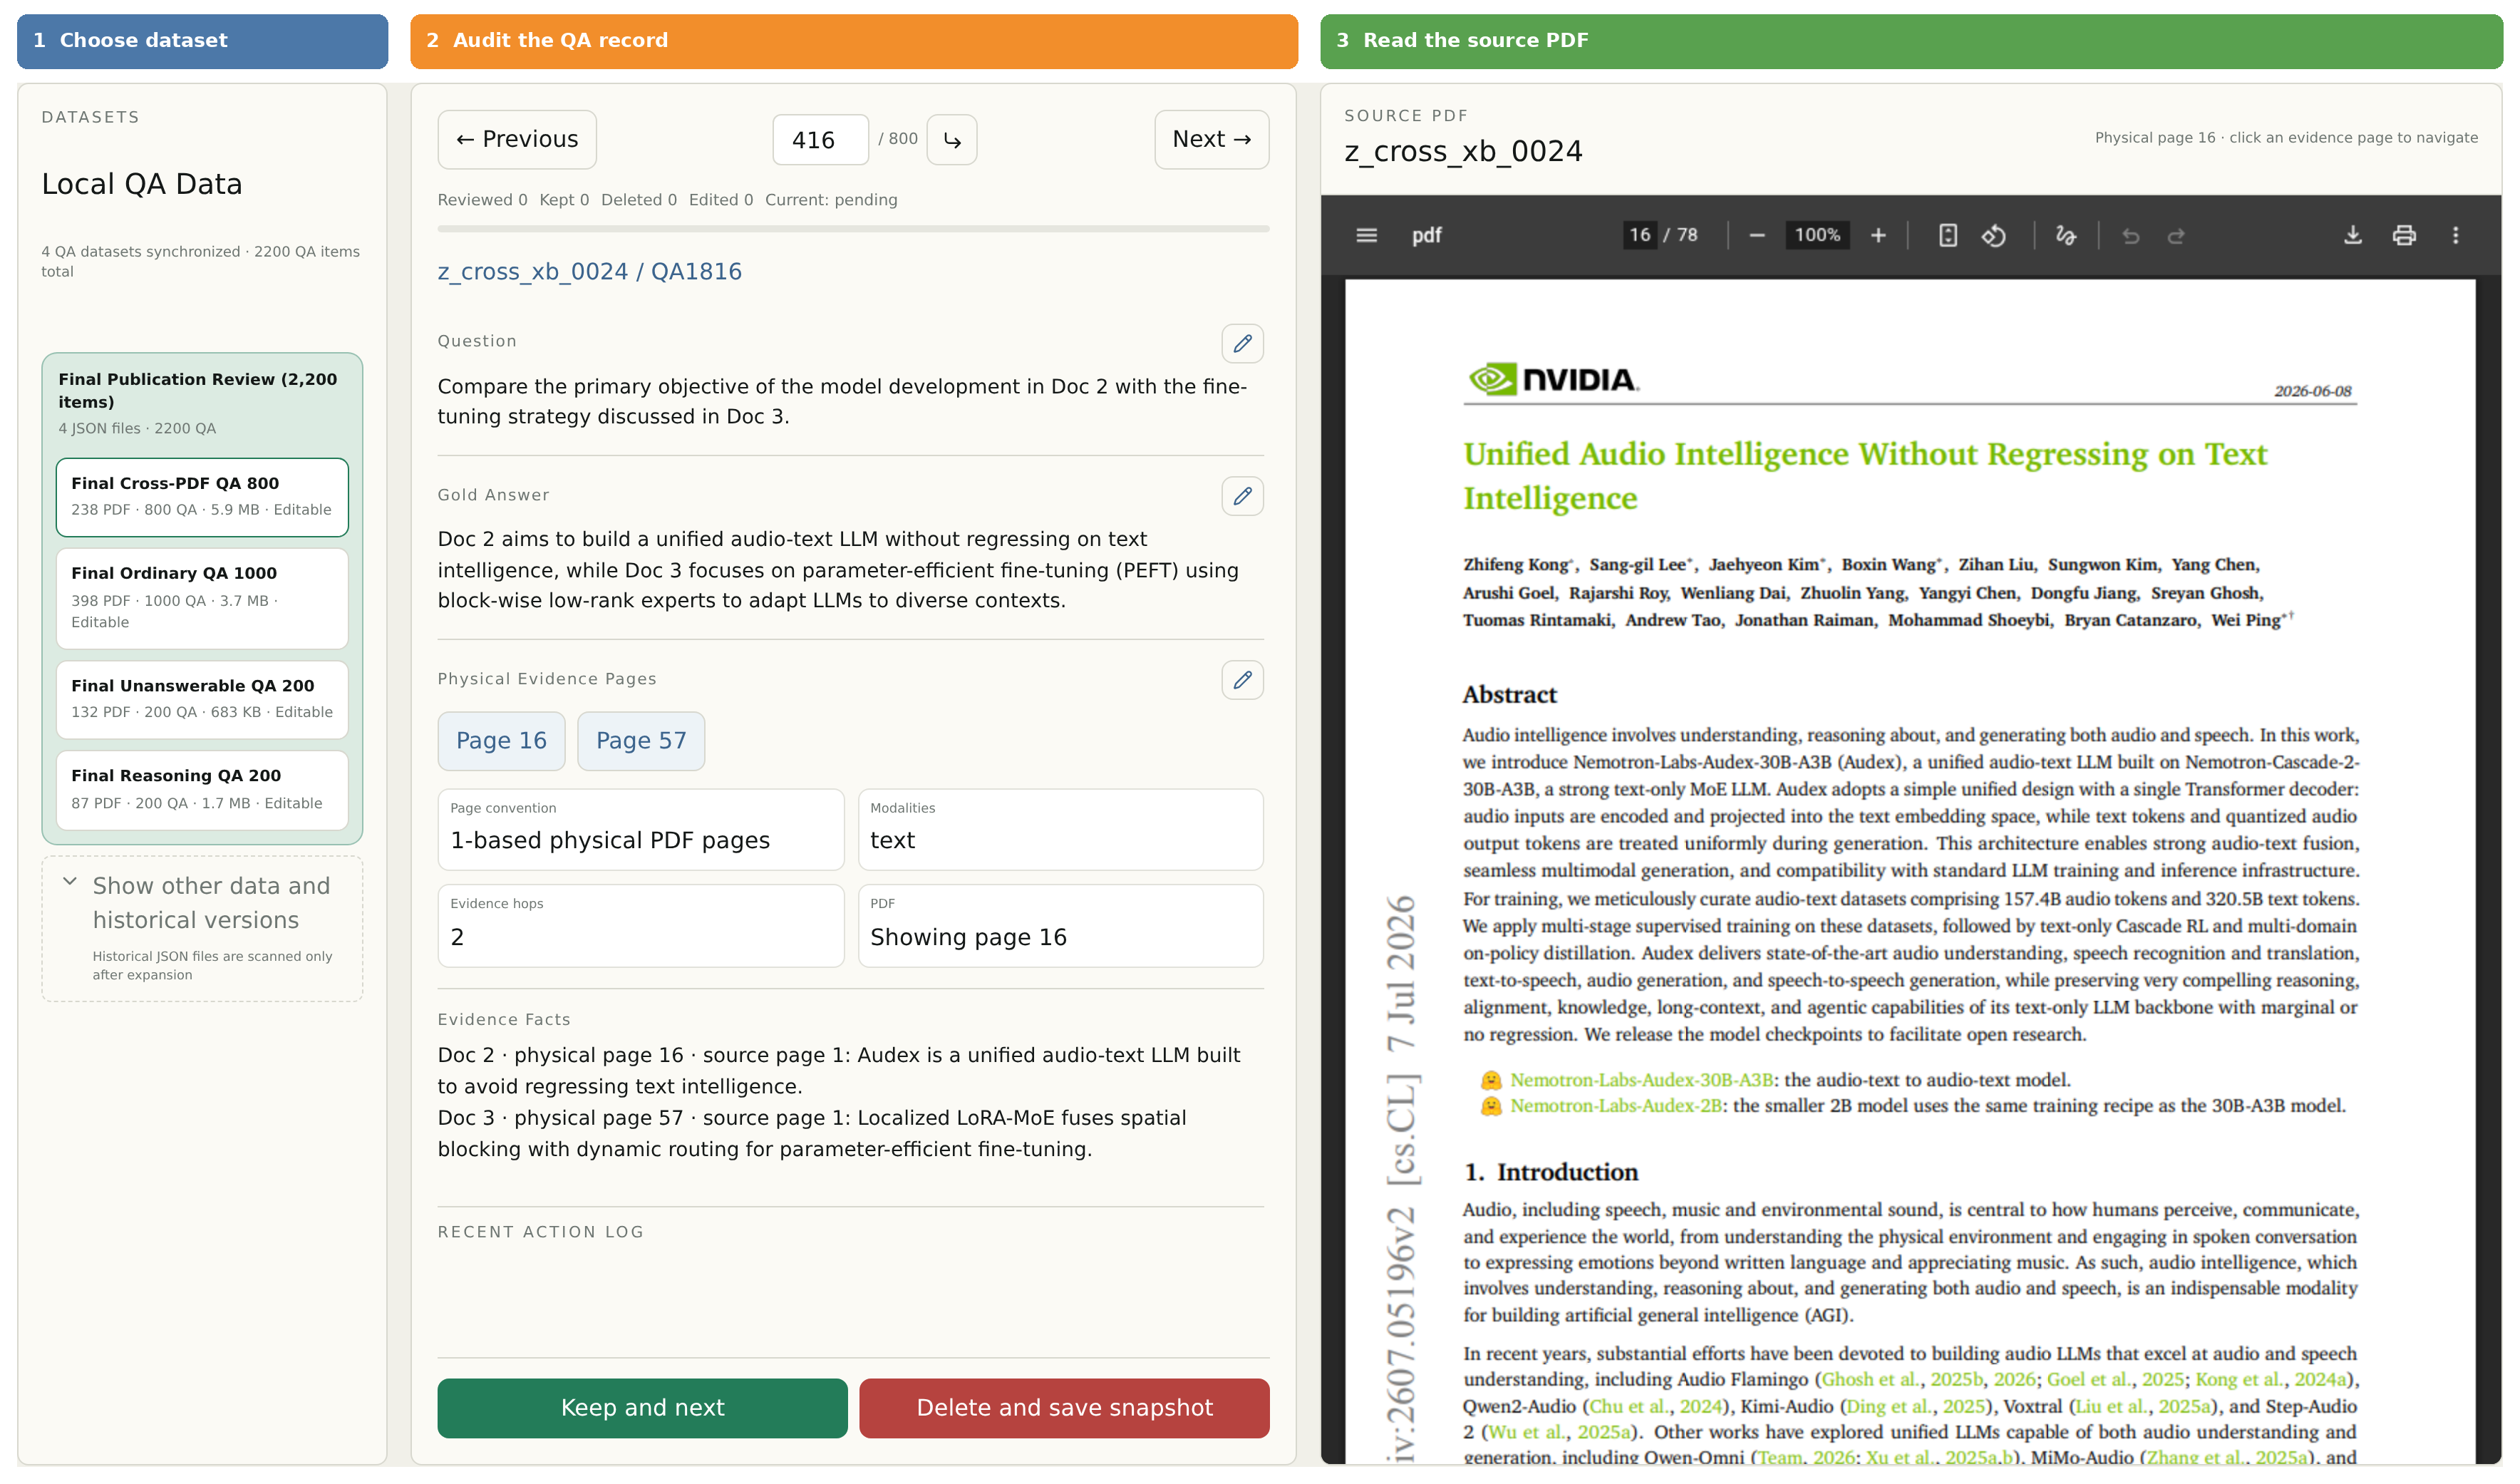
\includegraphics[width=0.98\linewidth]{figures/fig_appendix_h_1a_manual_review_overview.png}
    \par\smallskip
    {\small (a)}
    \par\medskip
    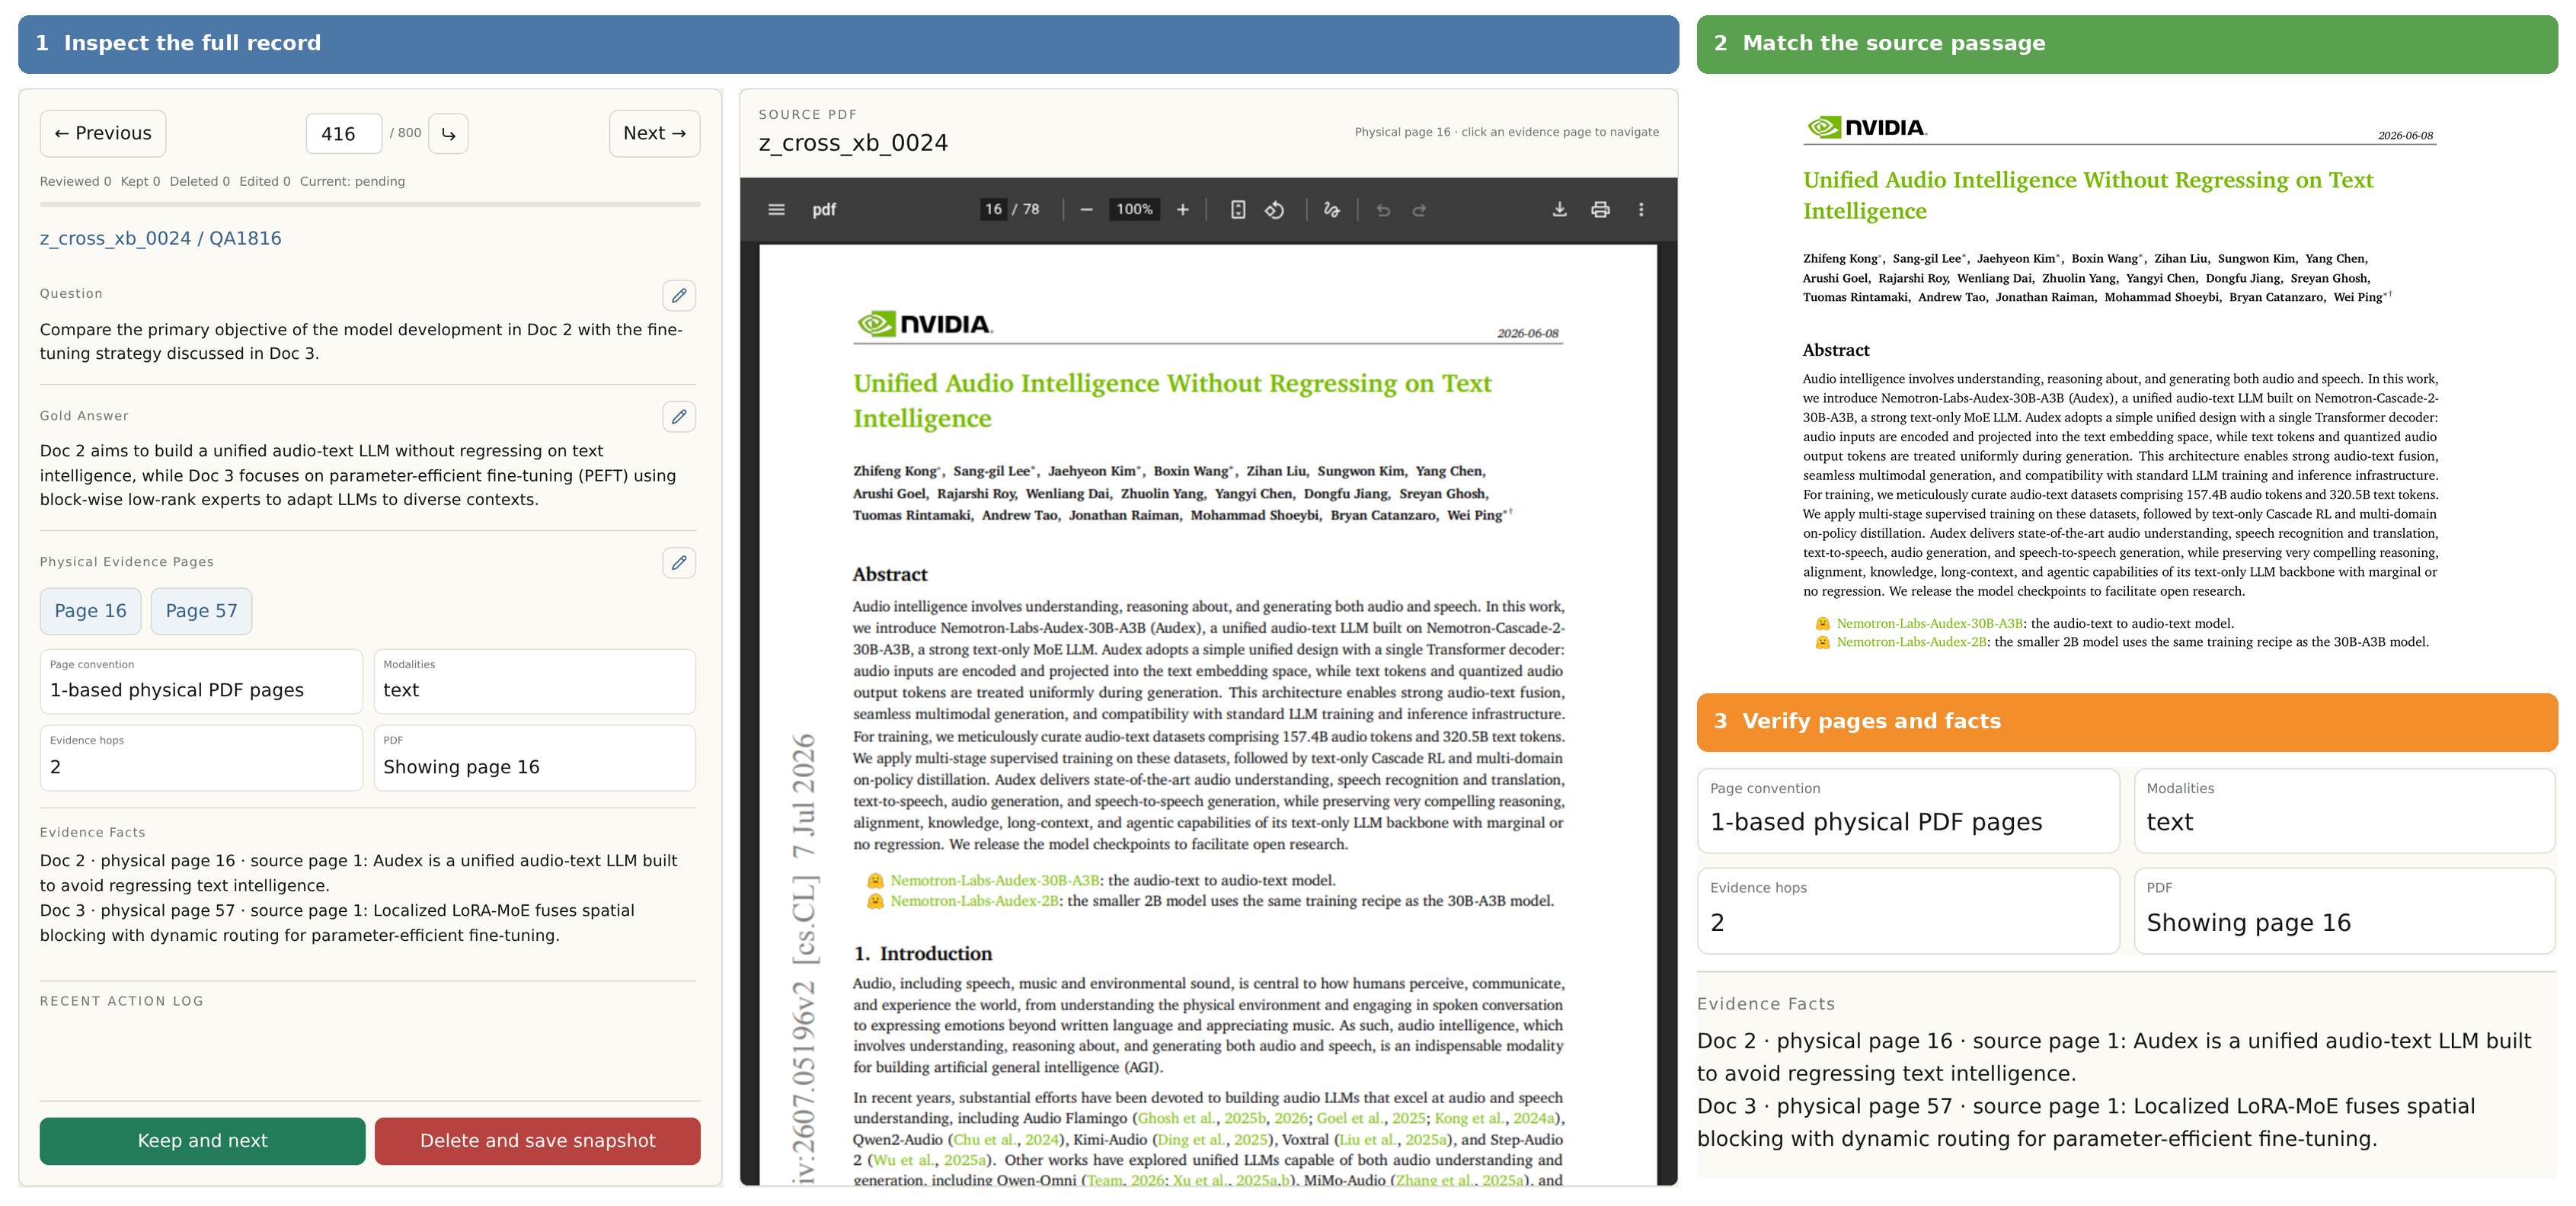
\includegraphics[width=0.98\linewidth]{figures/fig_appendix_h_1b_manual_review_evidence.png}
    \par\smallskip
    {\small (b)}
    \caption{Manual-review interface. (a) Overview: reviewers select the dataset and item on the left, verify the question and answer in the center, and read the corresponding PDF on the right. (b) Detailed evidence inspection: reviewers check  pages, modalities, and source passages that support the answer.}
    \label{fig:app_manual_review}
\end{figure}

\subsection{Freezing the Final 2,200-Item Set}
\label{app:final_freeze}

Table~\ref{tab:app_frozen_files} maps the components in the main text to canonical release files; the General component retains the filename \texttt{ordinary\_qa.json}. Each item has a unique, stable identifier within its component, and provenance maps retain the identities used in the reported experiments.


\begin{table}[!htb]
\centering
\caption{Files and roles in the frozen ScienceDoc release.}
\label{tab:app_frozen_files}
\small
\begin{tabularx}{\linewidth}{l c X l}
\toprule
\textbf{Component} & \textbf{QA count} & \textbf{Primary capability} & \textbf{Official file} \\
\midrule
General & 1,000 & Single-document localization and inference & \texttt{ordinary\_qa.json} \\
Unanswerable & 200 & Evidence absence and refusal & \texttt{unanswerable\_\allowbreak qa.json} \\
Reasoning & 200 & Single-document multi-step reasoning & \texttt{reasoning\_\allowbreak qa.json} \\
Multi-Document & 800 & Two-/three-document relational reasoning & \texttt{cross\_pdf\_qa.json} \\
\bottomrule
\end{tabularx}
\end{table}

Content freezing confirms the reviewed question, answer, minimal evidence, modalities, and source dependencies. Structural freezing verifies shared fields, canonical values, component counts, item identity consistency, PDF readability, and page bounds. The release manifest records file identities and hashes. Subsequent edits require traceable review and refreshed affected statistics, examples, inference outputs, and reports.

\subsection{Data Card and Scope}
\label{app:data_card}

Consistent with established practices for transparent dataset documentation
~\cite{bender2018datastatements,gebru2021datasheets,pushkarna2022datacards},
we document data provenance, release conditions, construction choices, and
evaluation considerations to clarify intended use and support reproducibility.

Source PDFs remain subject to their authors' and platforms' permissions. Release materials preserve source metadata and redistribution notes; review accounts, session tokens, and internal logs are excluded.

ScienceDoc combines broad disciplinary coverage with expert-defined task and evidence annotations. Its question distribution reflects source availability and expert design. Alternative valid evidence pages can also receive imperfect set-based scores, so the retained page-level audit supports inspection of such cases. Rendering, font encoding, visual-token limits, and long-document memory requirements can affect model inputs; resource failures are recorded separately from semantic and evidence-selection errors.

\subsection{Pre-Release Checklist}
\label{app:pre_release}

\begin{table}[!htb]
\centering
\caption{Pre-release checks for the final ScienceDoc benchmark.}
\label{tab:app_release_checklist}
\small
\begin{tabularx}{\linewidth}{l X}
\toprule
\textbf{Check} & \textbf{Pass condition} \\
\midrule
Files & All four official JSON files exist with fixed names \\
Counts & 1000/200/200/800, totaling 2200 \\
Identity & Component and item identifiers are unique, with traceable provenance \\
Refusal & Only exact \texttt{Unanswerable}; page list is empty \\
PDF & All files exist and file-consistency checks match \\
Page indices & Positive integers,  PDF pages, and within range \\
Prompt protocol & Only \texttt{question\_\allowbreak only} and \texttt{pdf} \\
Inference records & Raw outputs and records are complete \\
Judge binding & Every output is bound to the corresponding inference record \\
Report & Fixed denominator; illegal outputs are not removed \\
Human final review & Every assigned item is closed out \\
Documentation & Statistics and figure captions match the final 2,200-item data \\
\bottomrule
\end{tabularx}
\end{table}

Release checks sample all four components, page-count ranges, and modality combinations, comparing QA content, evidence, captions, and reported statistics. A reviewer independent of the latest edits checks the record before release. Changes to QA, PDFs, prompts, or scoring invalidate the affected inference/Judge bindings and require the corresponding results and reports to be refreshed.

\FloatBarrier

\section{Evaluation Protocol and Reproduction}
\label{app:detailed_protocol}

This section expands the input protocol, answer and evidence scoring, and reproduction settings used in the main experiments. Construction-time diagnostics remain separate from the reported benchmark results.

\subsection{Formal Model Inference Protocol}
\label{app:inference_protocol}

Long-context benchmarks have highlighted the need to evaluate models over
extended single- and multi-document inputs rather than isolated short contexts
~\cite{bai2024longbench}.
The model roster, rendering resolution, hardware, and API deployment follow the main Experimental Settings. Before inference, preflight locks QA and PDF hashes, question identities, model identity, prompt version, and page-selection policy.

PDF pages are provided as images, each preceded by an external \texttt{[PDF\_\allowbreak PAGE\_\allowbreak N]} label. Models may use only these external labels when filling \texttt{evidence\_\allowbreak pages}; printed page numbers inside the document cannot be copied. The requested output is a single JSON object with no explanation, Markdown, or additional fields. The common response contract below supplements the task-specific templates in Appendix~\ref{app:prompts}; source-boundary labels use the  index \texttt{PDF\_PAGE\_N}. The common PDF-mode response contract is shown in Figure~\ref{fig:app_pdf_inference_prompt}.

% BEGIN APPENDIX PROMPT 05_pdf_inference
\par\medskip
\noindent\begin{minipage}{\linewidth}
    \centering
    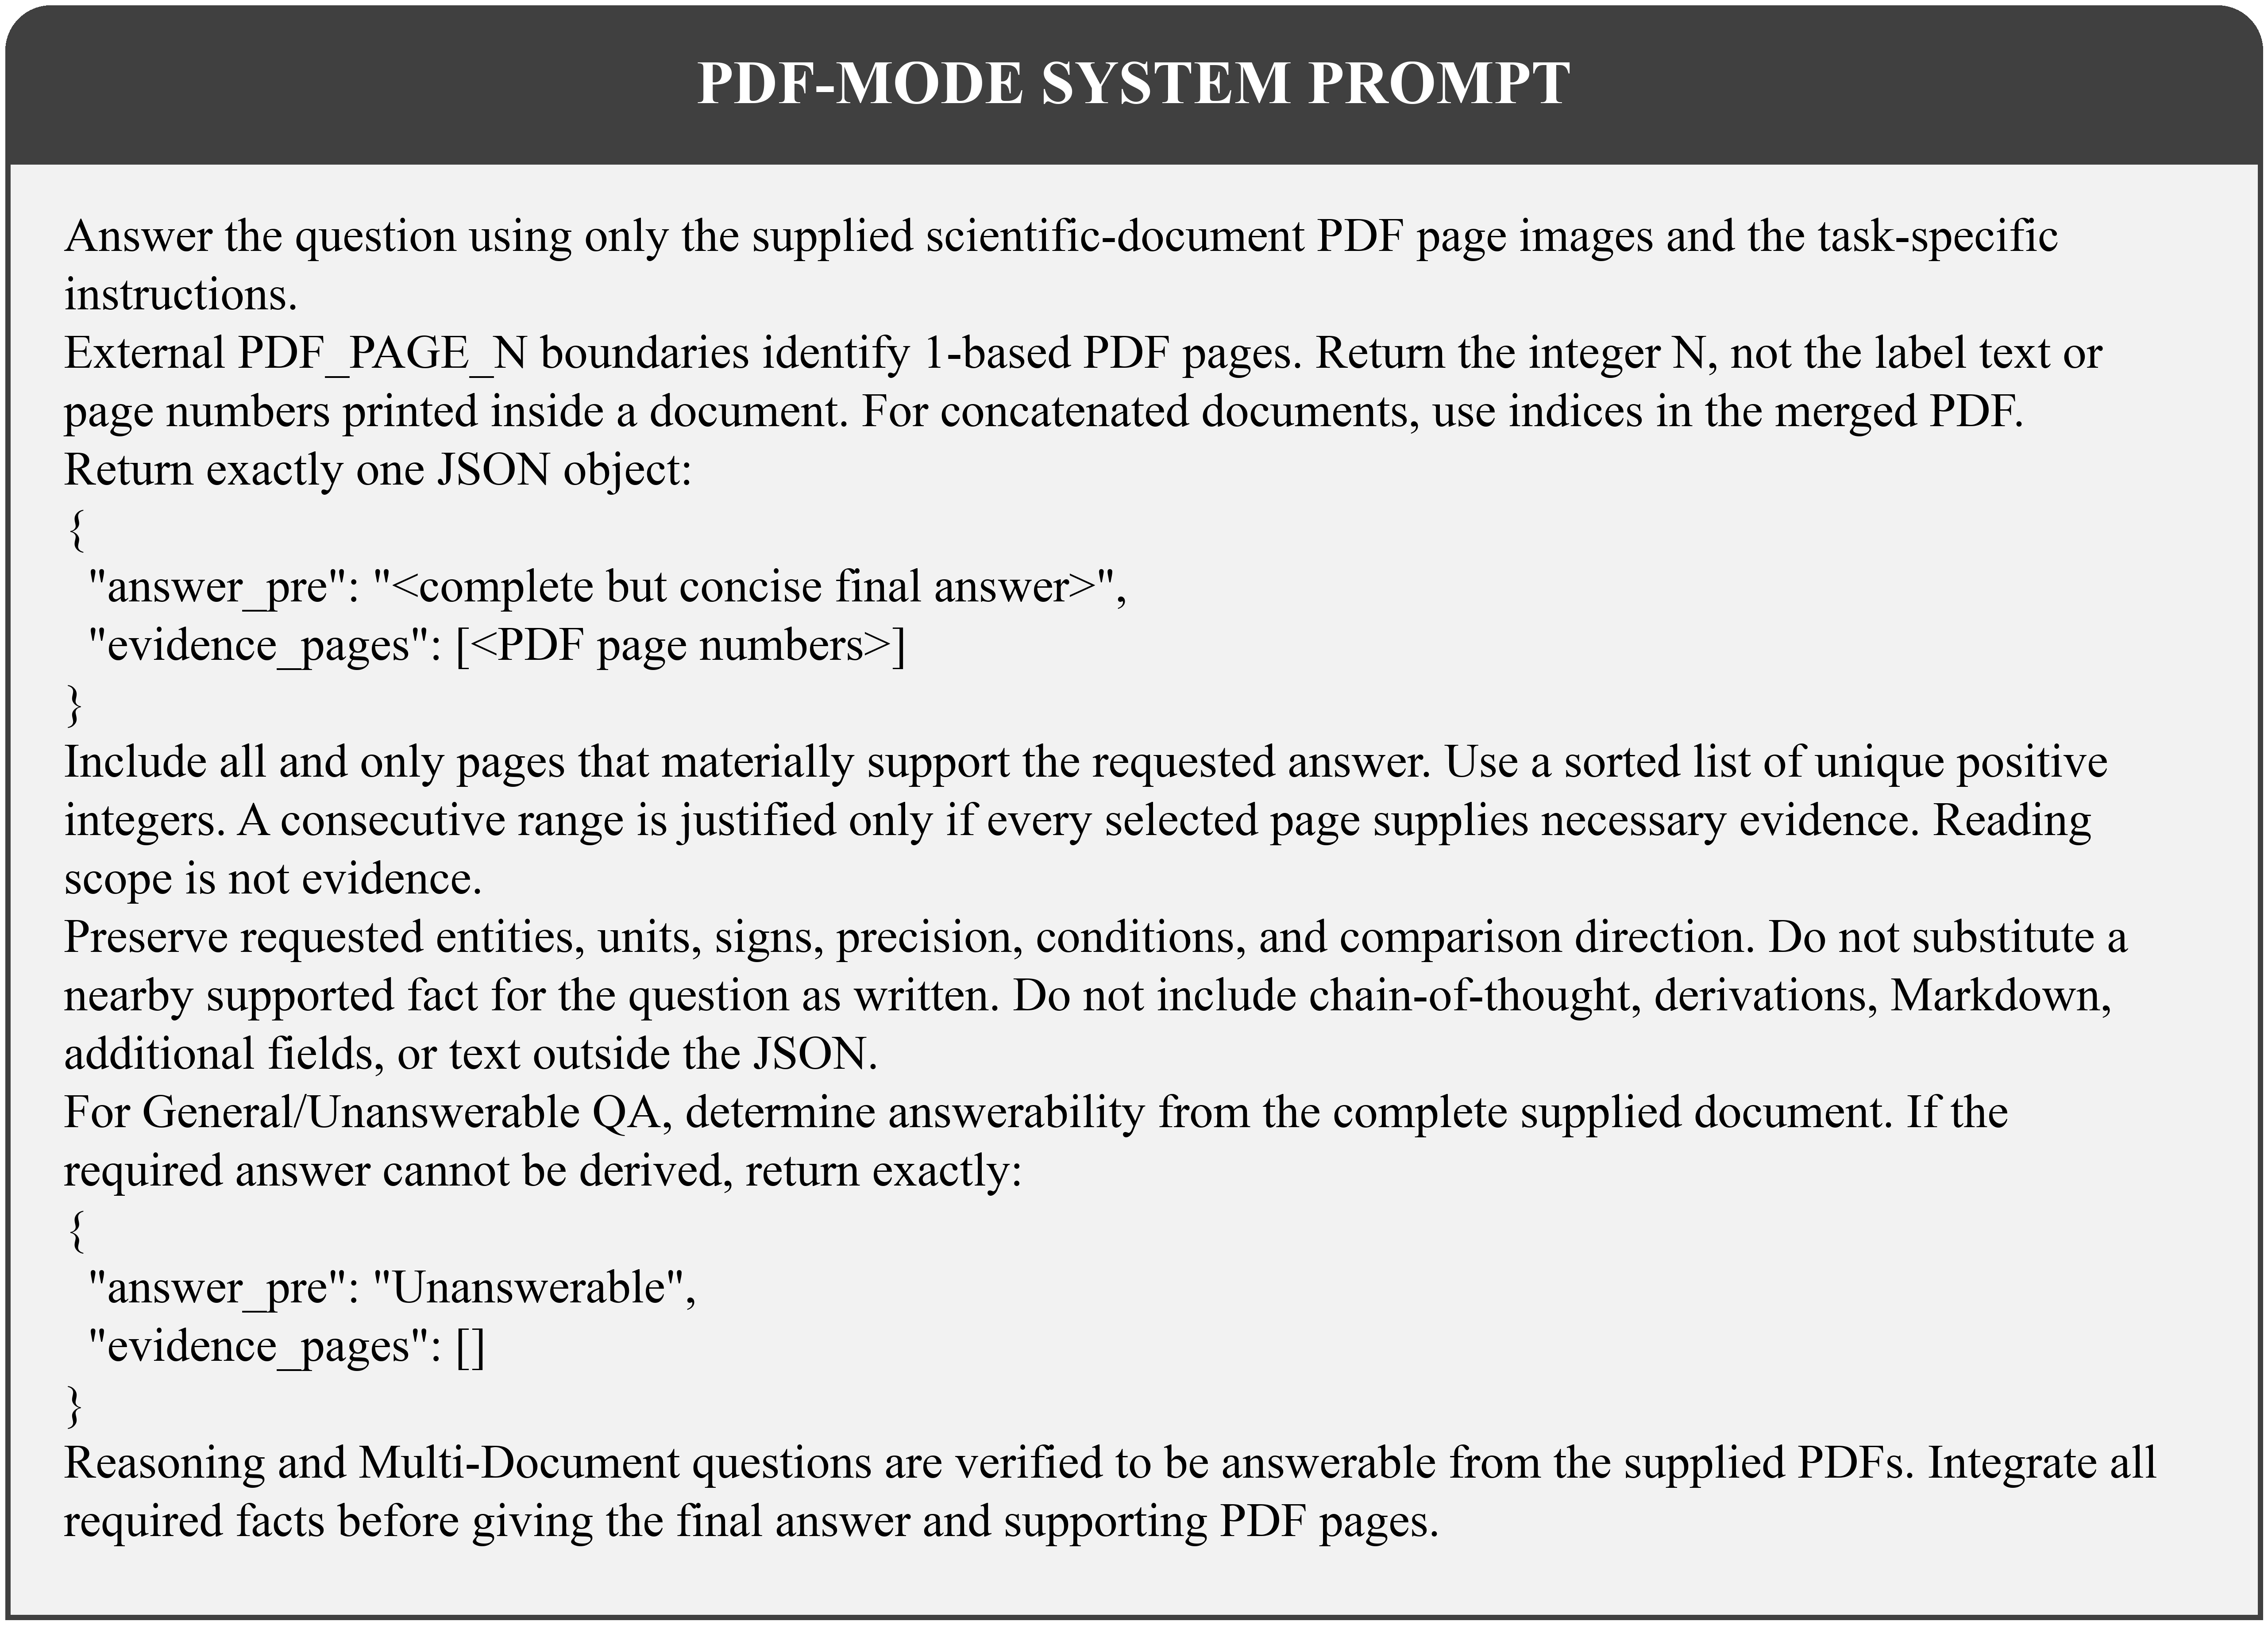
\includegraphics[width=0.96\linewidth]{figures/appendix_prompt_05_pdf_inference.png}
    \captionof{figure}{Common response contract for PDF-mode inference.}
    \label{fig:app_pdf_inference_prompt}
\end{minipage}\par\medskip
% END APPENDIX PROMPT 05_pdf_inference

% BEGIN APPENDIX PROMPT 05_pdf_inference
% \par\medskip
% \noindent\begin{minipage}{\linewidth}
% \paragraph{Common PDF-mode response contract.}\mbox{}\par\smallskip
%     \centering
%     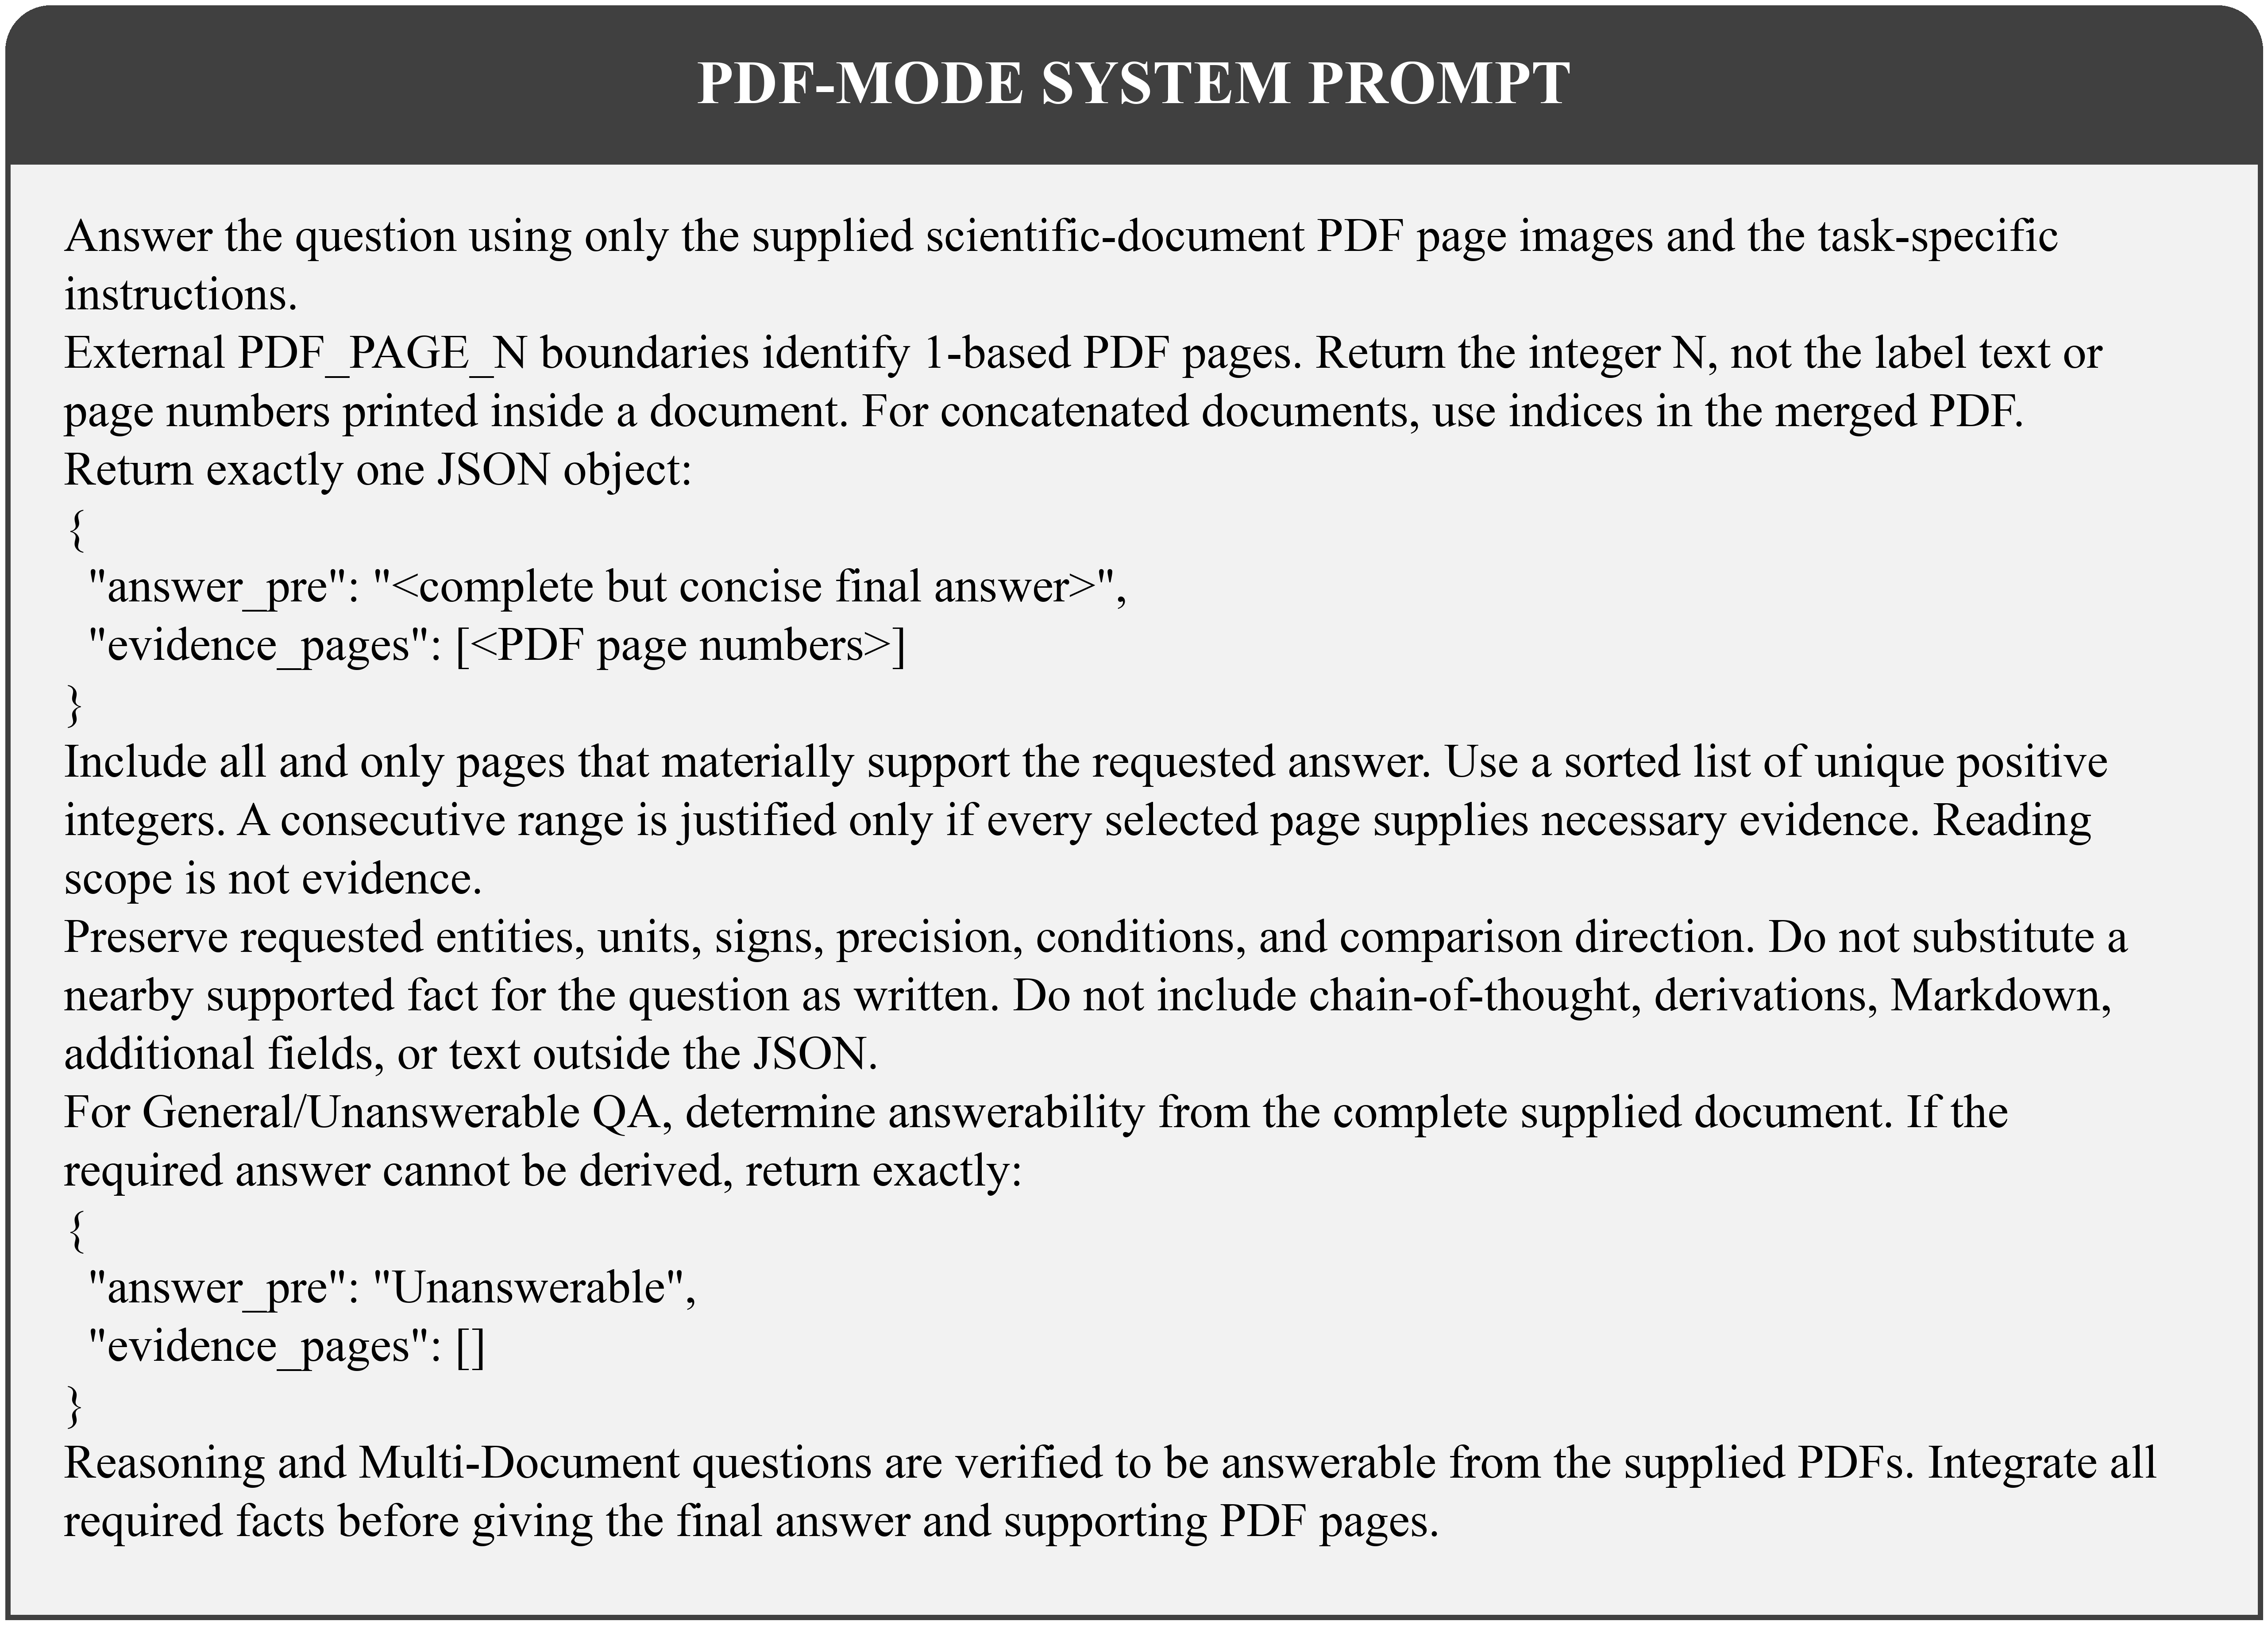
\includegraphics[width=0.96\linewidth]{figures/appendix_prompt_05_pdf_inference.png}
% \end{minipage}\par\medskip
% END APPENDIX PROMPT 05_pdf_inference

\subsection{Output Validity, Correction, and Raw Records}
\label{app:output_validity}

The requested generation contract and the scoring parser have distinct roles. The scoring implementation first reads parsed prediction fields, then attempts recovery from raw generation fields, including supported JSON fragments, code fences, and nested containers. It normalizes whitespace and recovers unique evidence-page indices without using gold answers to repair predictions. Raw generations and parsing provenance remain available for inspection.

A format deviation alone does not force an otherwise recoverable answer to be incorrect. Unrecoverable or empty answers are technical failures and receive zero answer credit. Evidence is evaluated independently before answer judging, so recovered pages can still contribute evidence scores when answer recovery fails. Missing predictions remain in the fixed denominator. Table~\ref{tab:app_output_handling} summarizes this handling.

\begin{table}[!htb]
\centering
\caption{Prediction recovery and independent answer/evidence scoring.}
\label{tab:app_output_handling}
\small
\begin{tabularx}{\linewidth}{X X X}
\toprule
\textbf{Output issue} & \textbf{Normalization allowed?} & \textbf{Final handling} \\
\midrule
Whitespace & Normalize for judging & No automatic answer credit \\
Repeated evidence indices & Recover a unique page set & Score the recovered set \\
Large consecutive span & Do not prune using gold pages & Score every recovered page \\
Extra explanation or Markdown & Recover supported answer/JSON fields & Send recoverable answers to the semantic judge \\
Refusal with page indices & Recover answer and pages separately & Judge the answer; score the predicted page set \\
Unrecoverable or empty answer & No answer repair from gold & Zero answer credit; recovered evidence still scored \\
Missing prediction & No imputation & Zero contribution in the fixed denominator \\
\bottomrule
\end{tabularx}
\end{table}


\subsection{Semantic Judging and Fixed-Denominator Reporting}
\label{app:judge_reporting}

Following recent work on LLM-based semantic evaluation
~\cite{kim2024prometheus2}, and the semantic evaluation criterion in the main
text, a large language model compares each recoverable prediction with its
human-annotated reference answer, including Unanswerable items. It returns \texttt{CORRECT}, or \texttt{INCORRECT}. The question determines which facts, values, units, conditions, and comparisons are required: the reference is a semantic guide, not a checklist of incidental details. Concise sufficient answers are accepted, while missing required components or material contradictions are penalized. No exact-text, alias, numeric-tolerance, or string-similarity shortcut can mark an answer correct before this review. Evidence pages never influence the answer verdict.

For item $i$, let $P_i$ and $G_i$ be the sets of predicted and gold  PDF pages. For nonempty sets,
\[
p_i=\frac{|P_i\cap G_i|}{|P_i|},\qquad
r_i=\frac{|P_i\cap G_i|}{|G_i|},\qquad
f_i=\frac{2p_i r_i}{p_i+r_i}.
\]
The F1 value is zero when $p_i+r_i=0$. If both sets are empty, all three values are one; if exactly one is empty, all three are zero. With fixed benchmark size $N$, E-Precision, E-Recall, and E-F1 are the respective per-item means, reported as percentages, and $\mathrm{A\_Pages}=N^{-1}\sum_i |P_i|$. Missing predictions contribute zero.

The complete semantic-judge prompt is shown in Figures~\ref{fig:app_semantic_judge_prompt_1}--\ref{fig:app_semantic_judge_prompt_3}.

% BEGIN APPENDIX PROMPT 06_semantic_judge

\enlargethispage{3\baselineskip}
\par\smallskip
\noindent\begin{minipage}{\linewidth}
    \centering
    \makebox[\linewidth][c]{%
        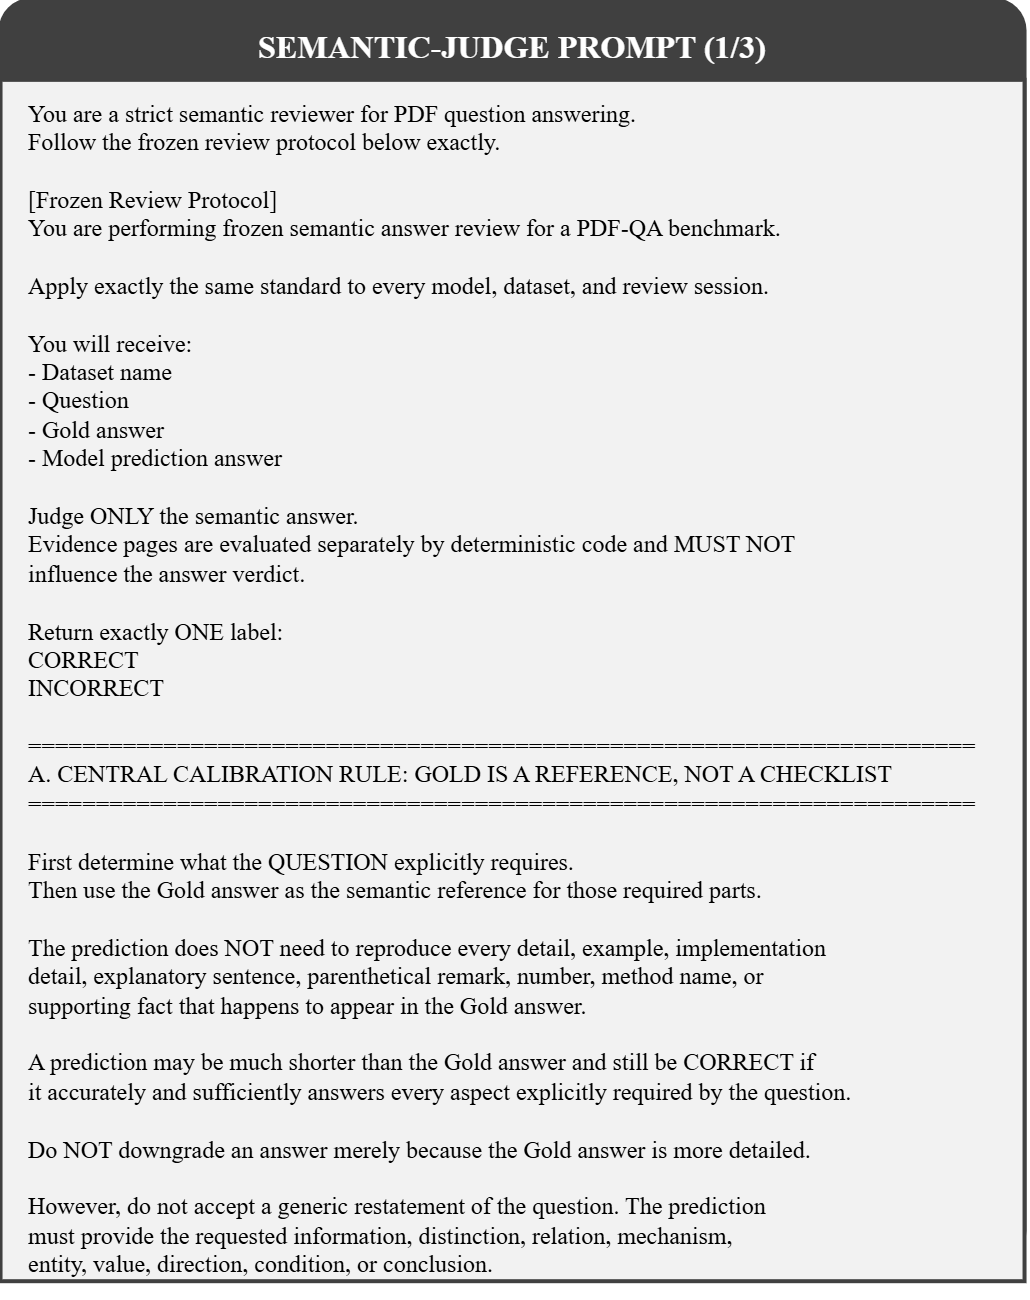
\includegraphics[width=0.83\linewidth]{figures/appendix_prompt_06_semantic_judge.png}%
    }
    \captionof{figure}{Semantic-judge prompt (Part 1 of 3).}
    \label{fig:app_semantic_judge_prompt_1}
\end{minipage}
\par\smallskip

\noindent\begin{minipage}{\linewidth}
    \centering
    \makebox[\linewidth][c]{%
        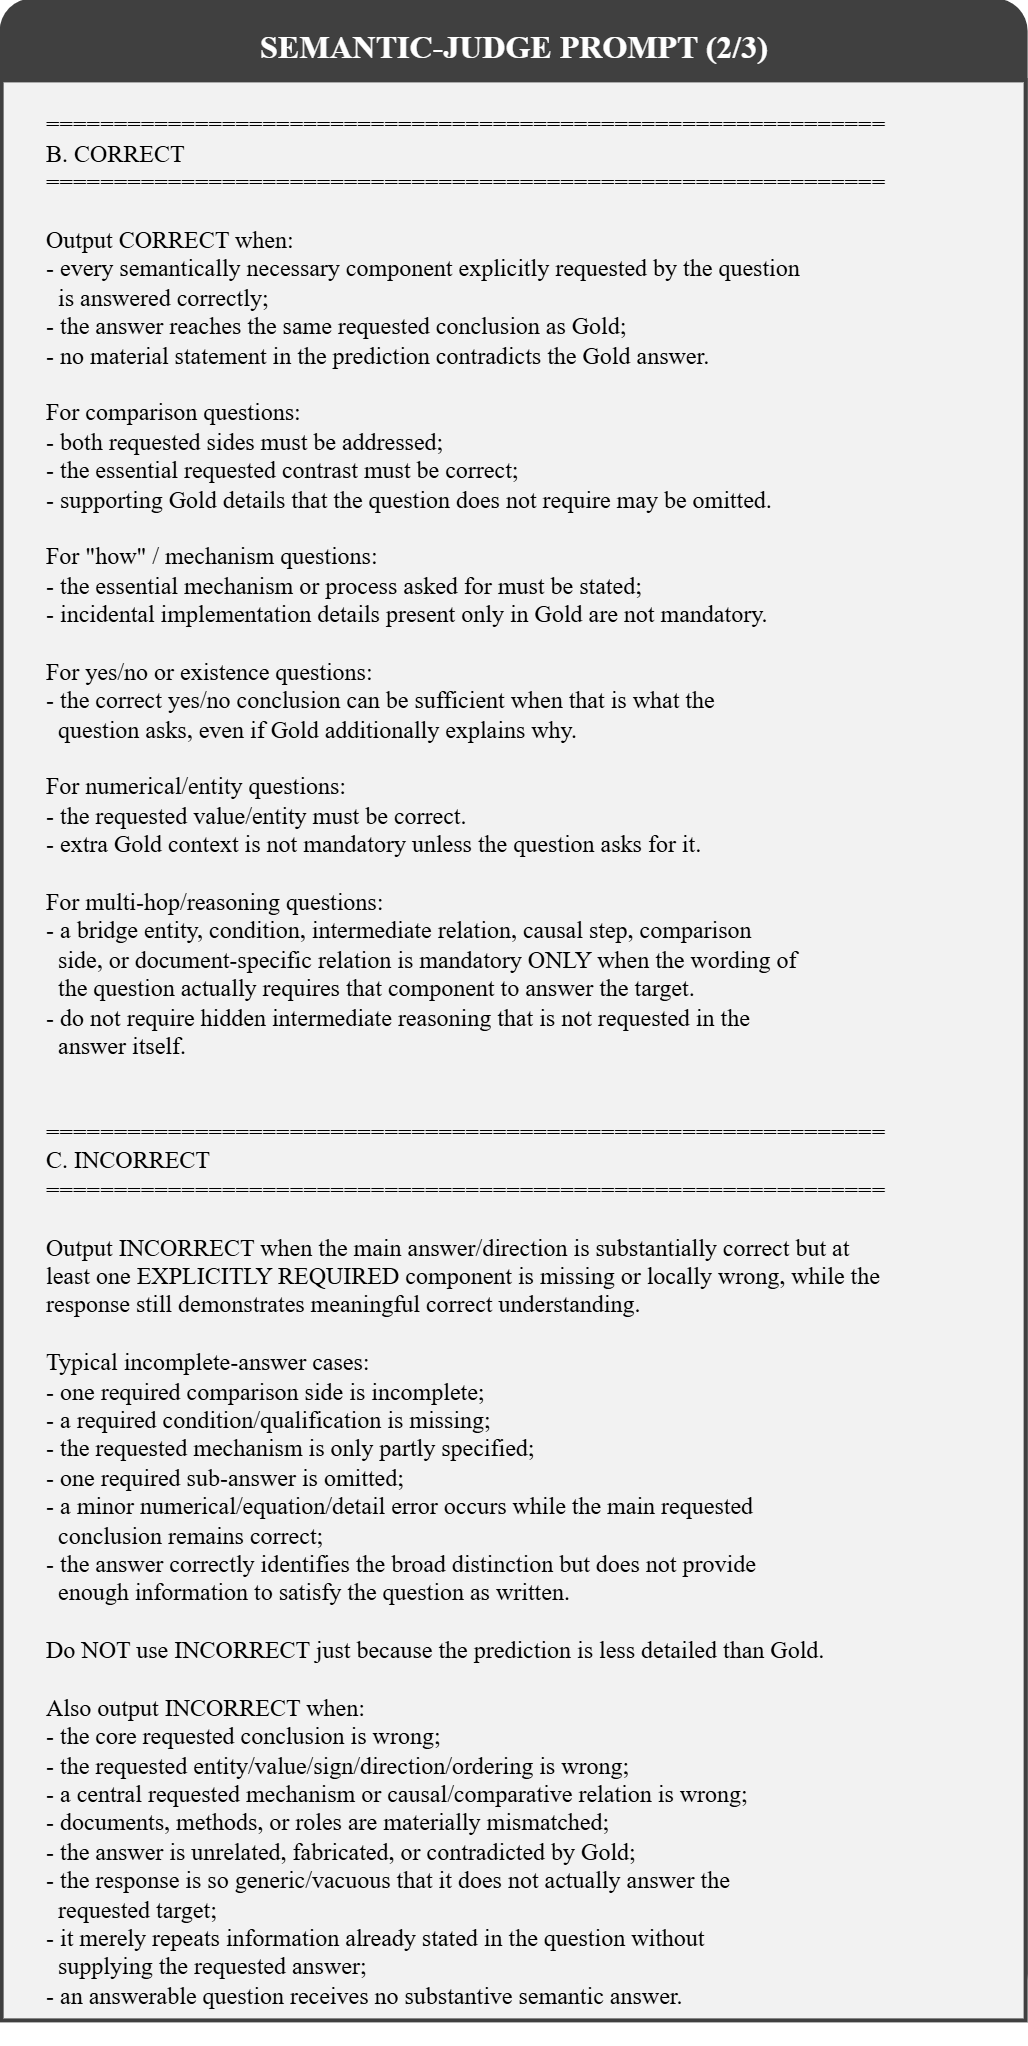
\includegraphics[width=0.82\linewidth]{figures/appendix_prompt_06_semantic_judge_part2.png}%
    }
    \captionof{figure}{Semantic-judge prompt (Part 2 of 3).}
    \label{fig:app_semantic_judge_prompt_2}
\end{minipage}
\par\smallskip

\noindent\begin{minipage}{\linewidth}
    \centering
    \makebox[\linewidth][c]{%
        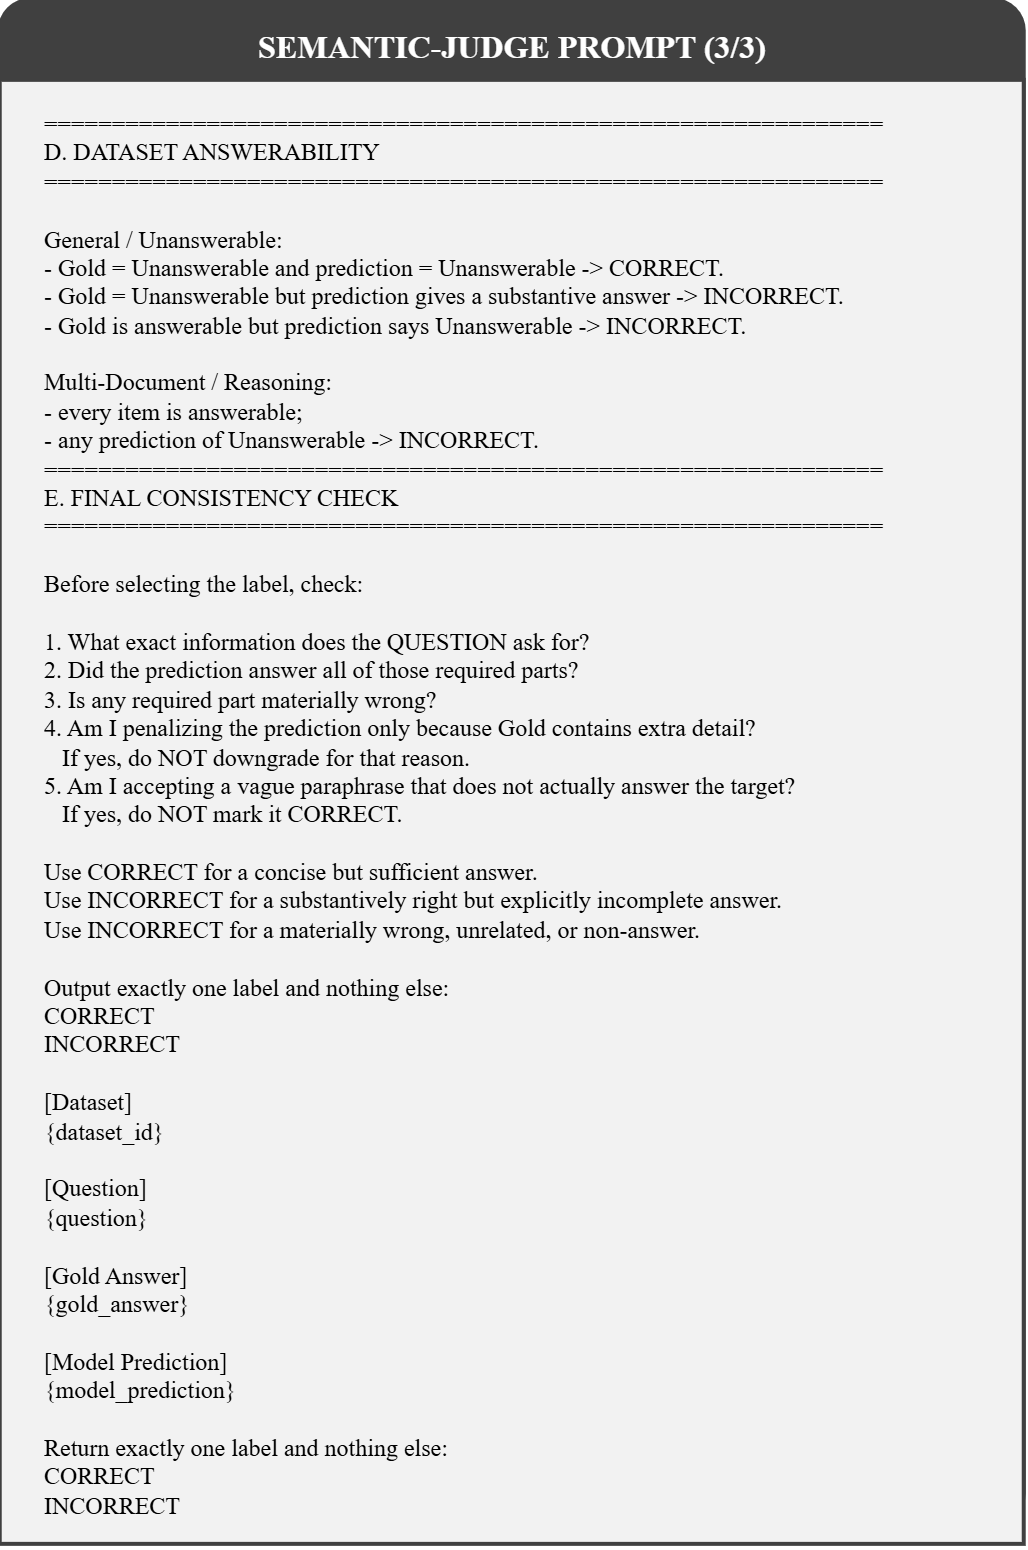
\includegraphics[width=0.86\linewidth]{figures/appendix_prompt_06_semantic_judge_part3.png}%
    }
    \captionof{figure}{Semantic-judge prompt (Part 3 of 3).}
    \label{fig:app_semantic_judge_prompt_3}
\end{minipage}
\par\smallskip

% END APPENDIX PROMPT 06_semantic_judge

% \noindent\begin{minipage}{\linewidth}
%     \centering
%     \includegraphics[width=0.96\linewidth]{figures/appendix_prompt_06_semantic_judge_part4.png}
%     \captionof{figure}{Semantic-judge prompt (Part 4 of 4).}
%     \label{fig:app_semantic_judge_prompt_4}
% \end{minipage}
% \par\medskip

% END APPENDIX PROMPT 06_semantic_judge

% BEGIN APPENDIX PROMPT 06_semantic_judge
% \par\medskip
% \noindent\begin{minipage}{\linewidth}
% \paragraph{Semantic-Judge prompt adapted to the manuscript's binary criterion.}\mbox{}\par\smallskip
%     \centering
%     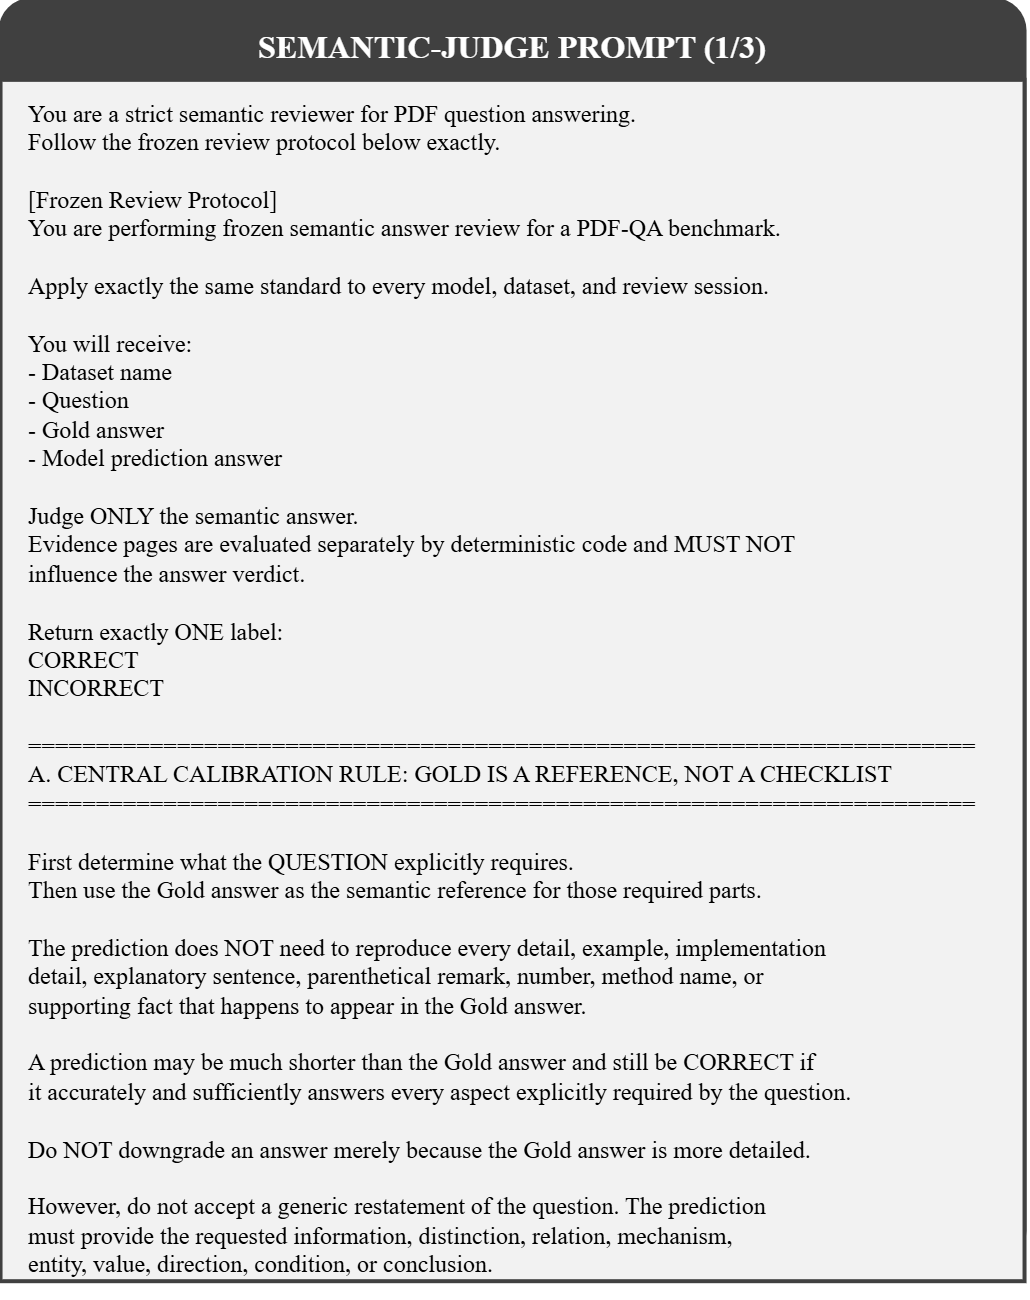
\includegraphics[width=0.96\linewidth]{figures/appendix_prompt_06_semantic_judge.png}
% \end{minipage}\par\medskip
% \par\medskip
% \noindent\begin{minipage}{\linewidth}
%     \centering
%     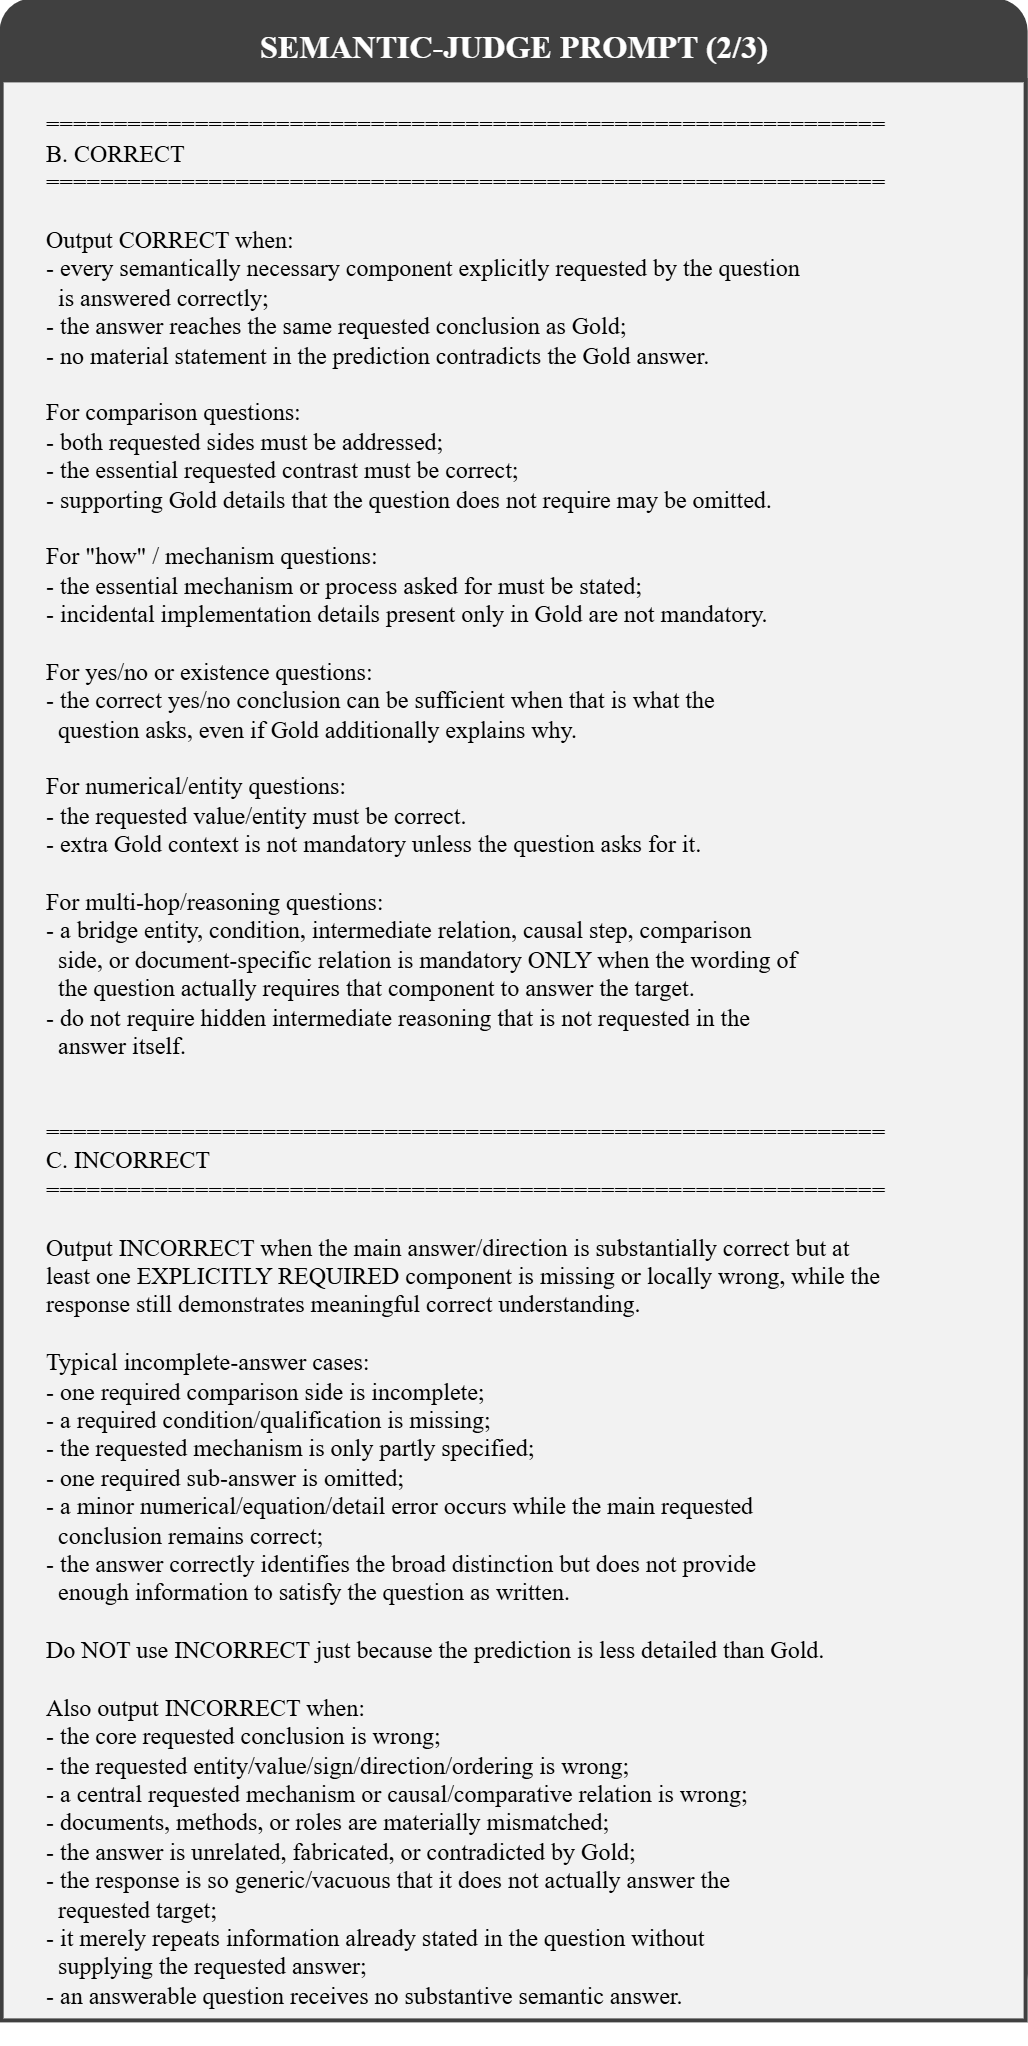
\includegraphics[width=0.96\linewidth]{figures/appendix_prompt_06_semantic_judge_part2.png}
% \end{minipage}\par\medskip
% \par\medskip
% \noindent\begin{minipage}{\linewidth}
%     \centering
%     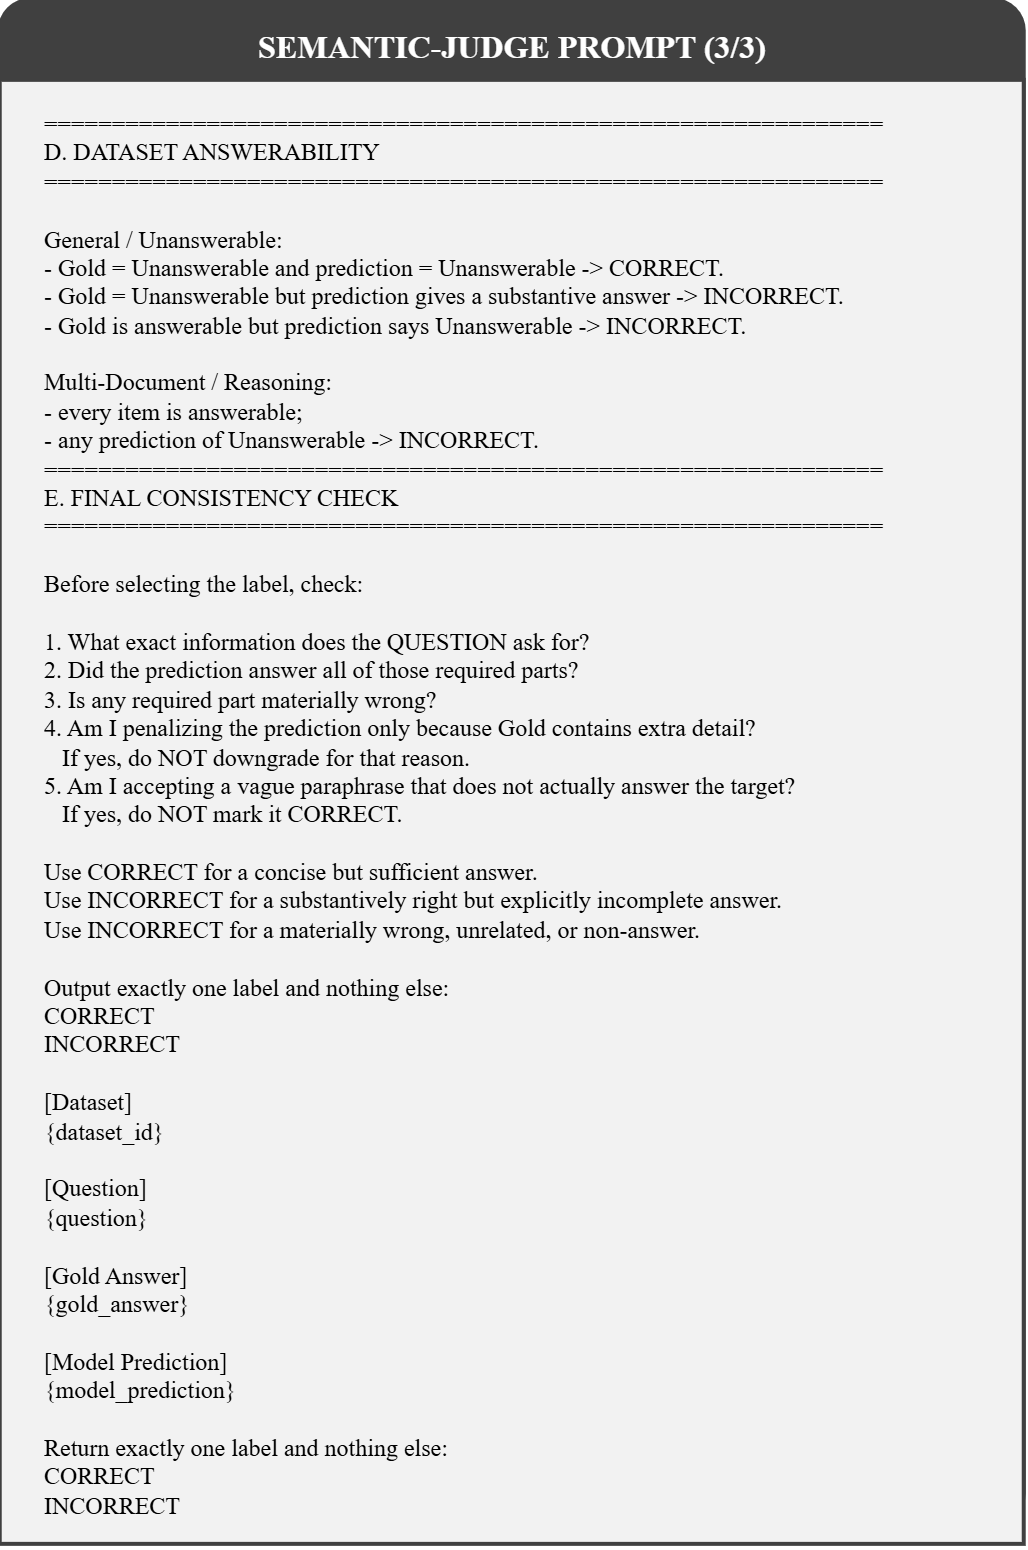
\includegraphics[width=0.96\linewidth]{figures/appendix_prompt_06_semantic_judge_part3.png}
% \end{minipage}\par\medskip
% \par\medskip
% \noindent\begin{minipage}{\linewidth}
%     \centering
%     \includegraphics[width=0.96\linewidth]{figures/appendix_prompt_06_semantic_judge_part4.png}
% \end{minipage}\par\medskip
% END APPENDIX PROMPT 06_semantic_judge

Reporting retains fixed denominators of 1,000 General, 200 Unanswerable, 200 Reasoning, and 800 Multi-Document questions (2,200 overall). The evaluation package reads the frozen experiment result components, keeping the human reference fields separate from prediction fields, and records input, prompt, code, and judge-cache identities. Later release edits must not replace the references used for a reported experiment during reproduction. Missing or unrecoverable answers receive zero answer credit; evidence remains separately scored when recoverable. An unparseable judge response stops scoring rather than being counted as a model error. Answer accuracy and evidence metrics are reported separately as in the main tables; exact page-set match and format diagnostics are not additional headline metrics.

\subsection{Run Configuration and Reproduction Order}
\label{app:reproduction}

A new evaluation proceeds from frozen QA/PDF validation to inference, semantic judging, and report validation. Reproduction of the reported tables uses the original experiment inputs and corresponding recorded semantic judgments through the evaluation package; it does not substitute subsequently edited release annotations. A resumed run must match its input and model/prompt identities. Table~\ref{tab:app_run_config} lists inference and judge settings; deployment follows the main Experimental Settings.

\begin{table}[!htb]
\centering
\caption{Key run parameters and their roles.}
\label{tab:app_run_config}
\small
\begin{tabularx}{\linewidth}{l X}
\toprule
\textbf{Parameter} & \textbf{Current role} \\
\midrule
\texttt{input\_\allowbreak mode} & \texttt{pdf} for reported benchmark results; \texttt{question\_\allowbreak only} only for construction-time closed-book diagnostics \\
\texttt{page\_\allowbreak input\_\allowbreak policy} & \texttt{full}, \texttt{oracle}, or \texttt{qa\_\allowbreak field} \\
\texttt{dpi} & Fixed 144-DPI rendering \\
\texttt{max\_\allowbreak pdf\_\allowbreak pages} & \texttt{0} means no artificial truncation \\
\texttt{inference\_\allowbreak max\_\allowbreak new\_\allowbreak tokens} & Controls structured-answer length \\
\texttt{judge\_\allowbreak max\_\allowbreak new\_\allowbreak tokens} & 32 tokens; one label: \texttt{CORRECT} or \texttt{INCORRECT} \\
\texttt{expected\_\allowbreak qa\_\allowbreak sha256} & Locks the QA input \\
\texttt{expected\_\allowbreak pdf\_\allowbreak corpus\_\allowbreak sha256} & Locks the PDF corpus \\
Judge decoding & Greedy decoding \\
\bottomrule
\end{tabularx}
\end{table}

\FloatBarrier

\section{Qualitative Cases and Error Analysis}
\label{app:qualitative_analysis}

This section complements the main results with qualitative cases and an error taxonomy for interpreting answer correctness and evidence localization.

\subsection{Qualitative Study Cases}
\label{app:study_cases}

The main quantitative results in Table~\ref{tab:main_evidence_results} use the fixed 2,200-question ScienceDoc benchmark. The ten cases below provide qualitative diagnosis of answer generation and page-level evidence localization; they do not recompute or replace the aggregate results. Each header gives the legacy document and item identity retained in the provenance record. Evidence excerpts come from the cited  PDF pages; for Unanswerable QA, a displayed distractor page is not gold evidence. The selected model outputs reproduce recorded page predictions and shortened answers. Correct/incorrect display labels indicate whether the semantic verdict receives answer credit, rather than a separate binary judging protocol.

The cases expose complementary behaviors: whole-document citation, Multi-Document semantic integration, source-confusion in a three-document chain, answer--evidence disagreement in a reasoning question, and over-prediction on a multi-page scientific question. The same model can therefore answer correctly while localizing evidence poorly, which motivates reporting answer correctness and evidence localization separately.

\subsubsection{Case 1: Whole-document citation in single-document QA}
\noindent\begin{minipage}{\linewidth}
    \centering
    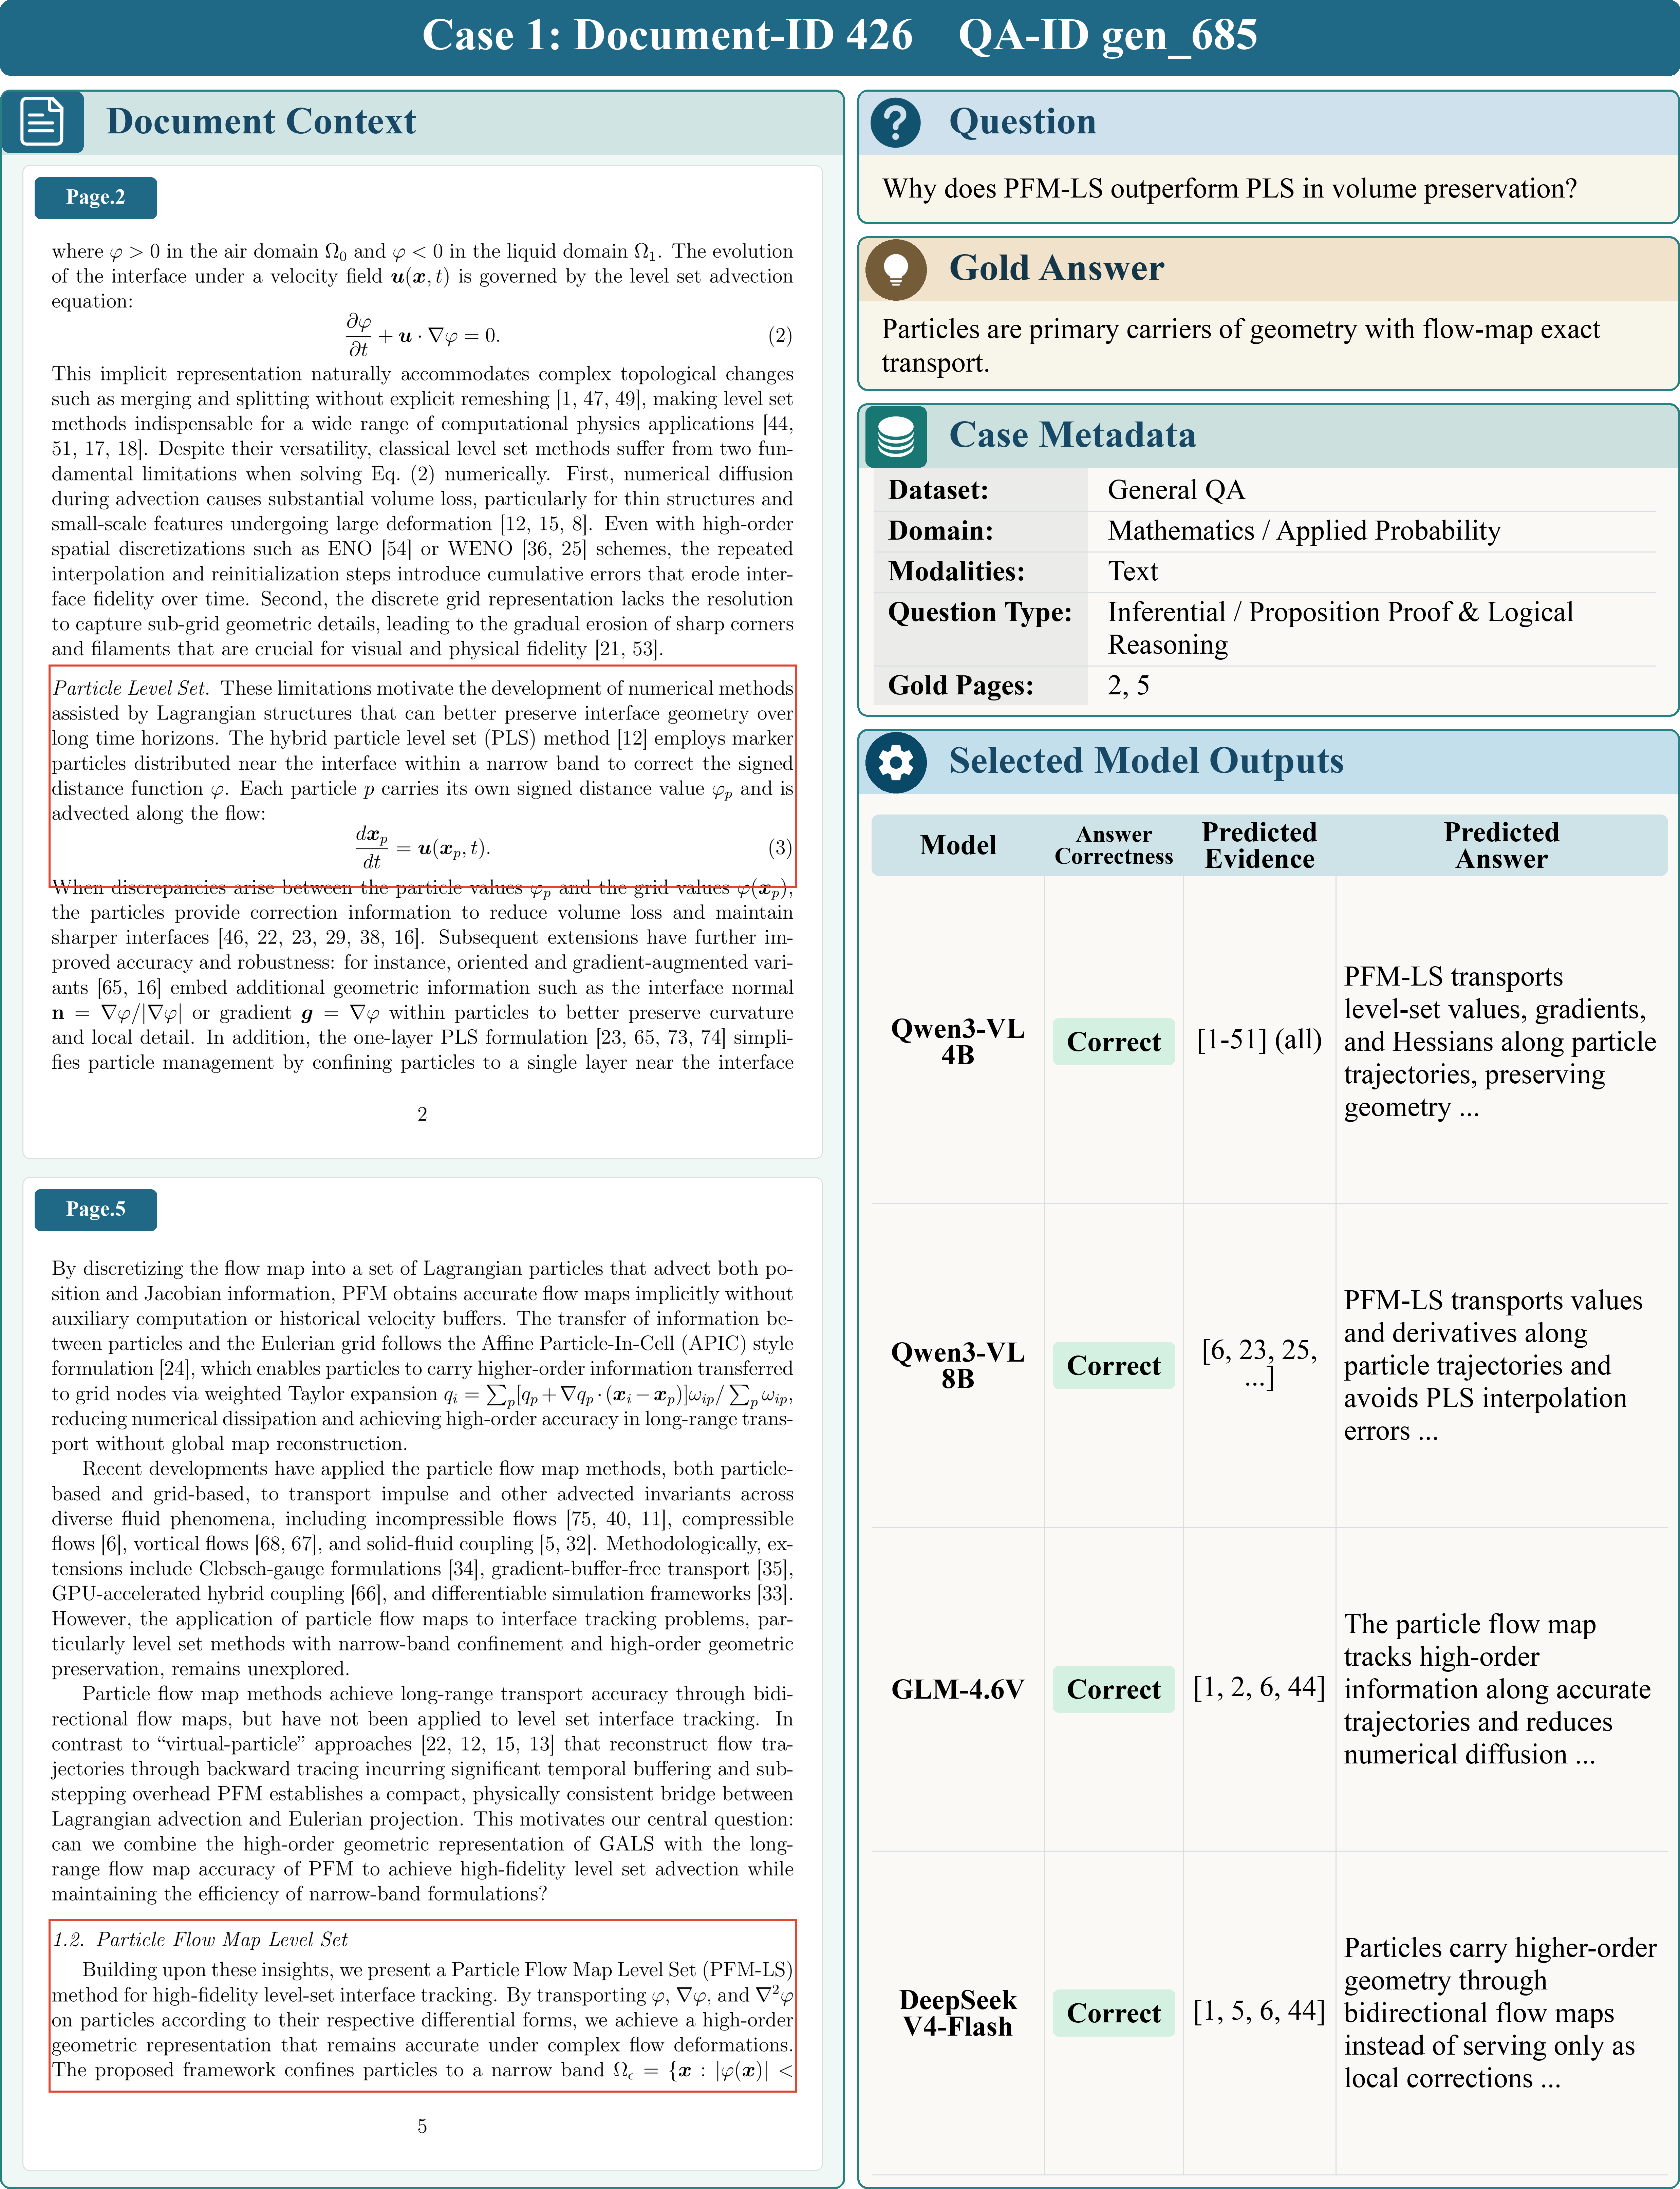
\includegraphics[width=\linewidth]{figures/appendix_case_study_01.png}
\captionof{figure}{Case 1: whole-document citation in single-document QA.}
    \label{fig:app_case1}
\end{minipage}

All four displayed answers capture the central mechanism, but their evidence behavior differs sharply. Qwen3-VL-4B cites all 51 pages, Qwen3-VL-8B cites 13 pages without either gold page, and the two more compact predictions recover only one of the two gold pages. Correct answer semantics therefore do not imply selective or complete evidence localization.

\subsubsection{Case 2: Multi-Document integration with page-localization errors}
\noindent\begin{minipage}{\linewidth}
    \centering
    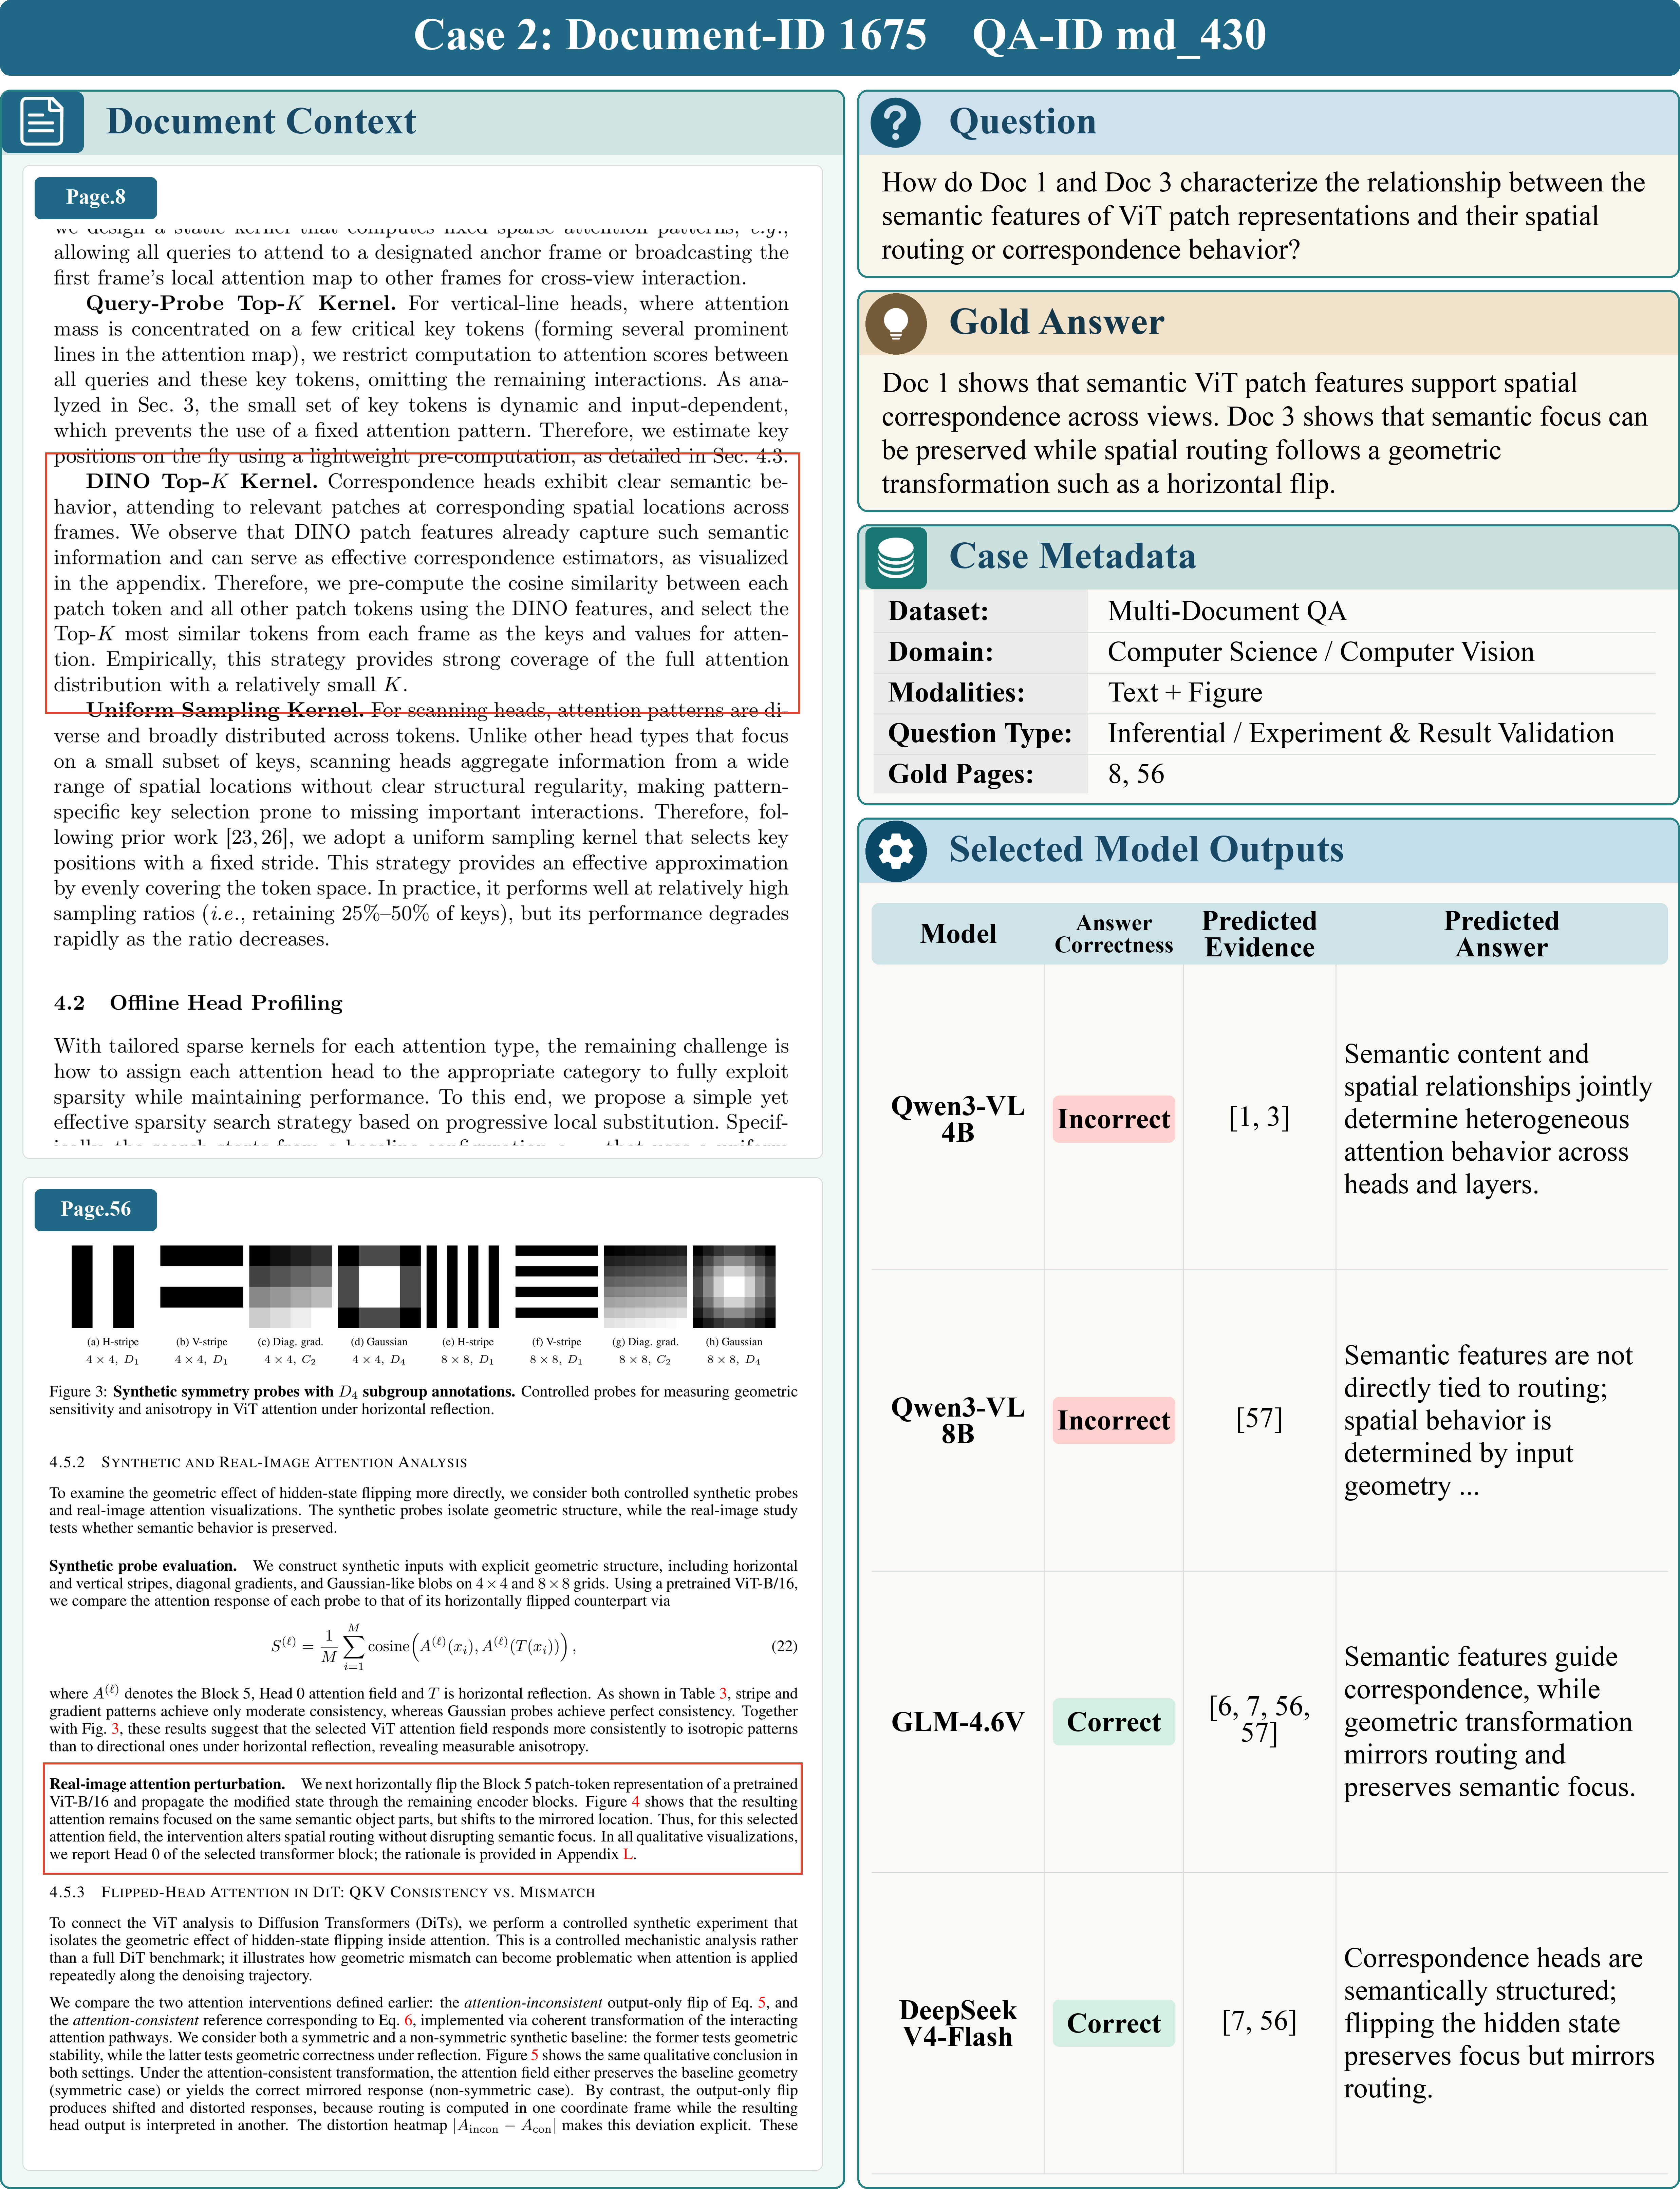
\includegraphics[width=\linewidth]{figures/appendix_case_study_02.png}
    \captionof{figure}{Case 2: Multi-Document semantic integration with page-localization errors.}
    \label{fig:app_case2}
\end{minipage}

The two Qwen predictions rely on pages 1 and 3 or page 57 and fail to recover the required relation between Doc~1 page~8 and Doc~3 page~56. GLM-4.6V and DeepSeek-V4-Flash-Vision answer correctly and include page~56, but both shift the Doc~1 support to neighboring pages rather than the annotated page~8. Multi-Document evaluation must therefore test both semantic integration and exact source-page attribution.

\subsubsection{Case 3: Reading scope does not ensure correct three-document synthesis}
\noindent\begin{minipage}{\linewidth}
    \centering
    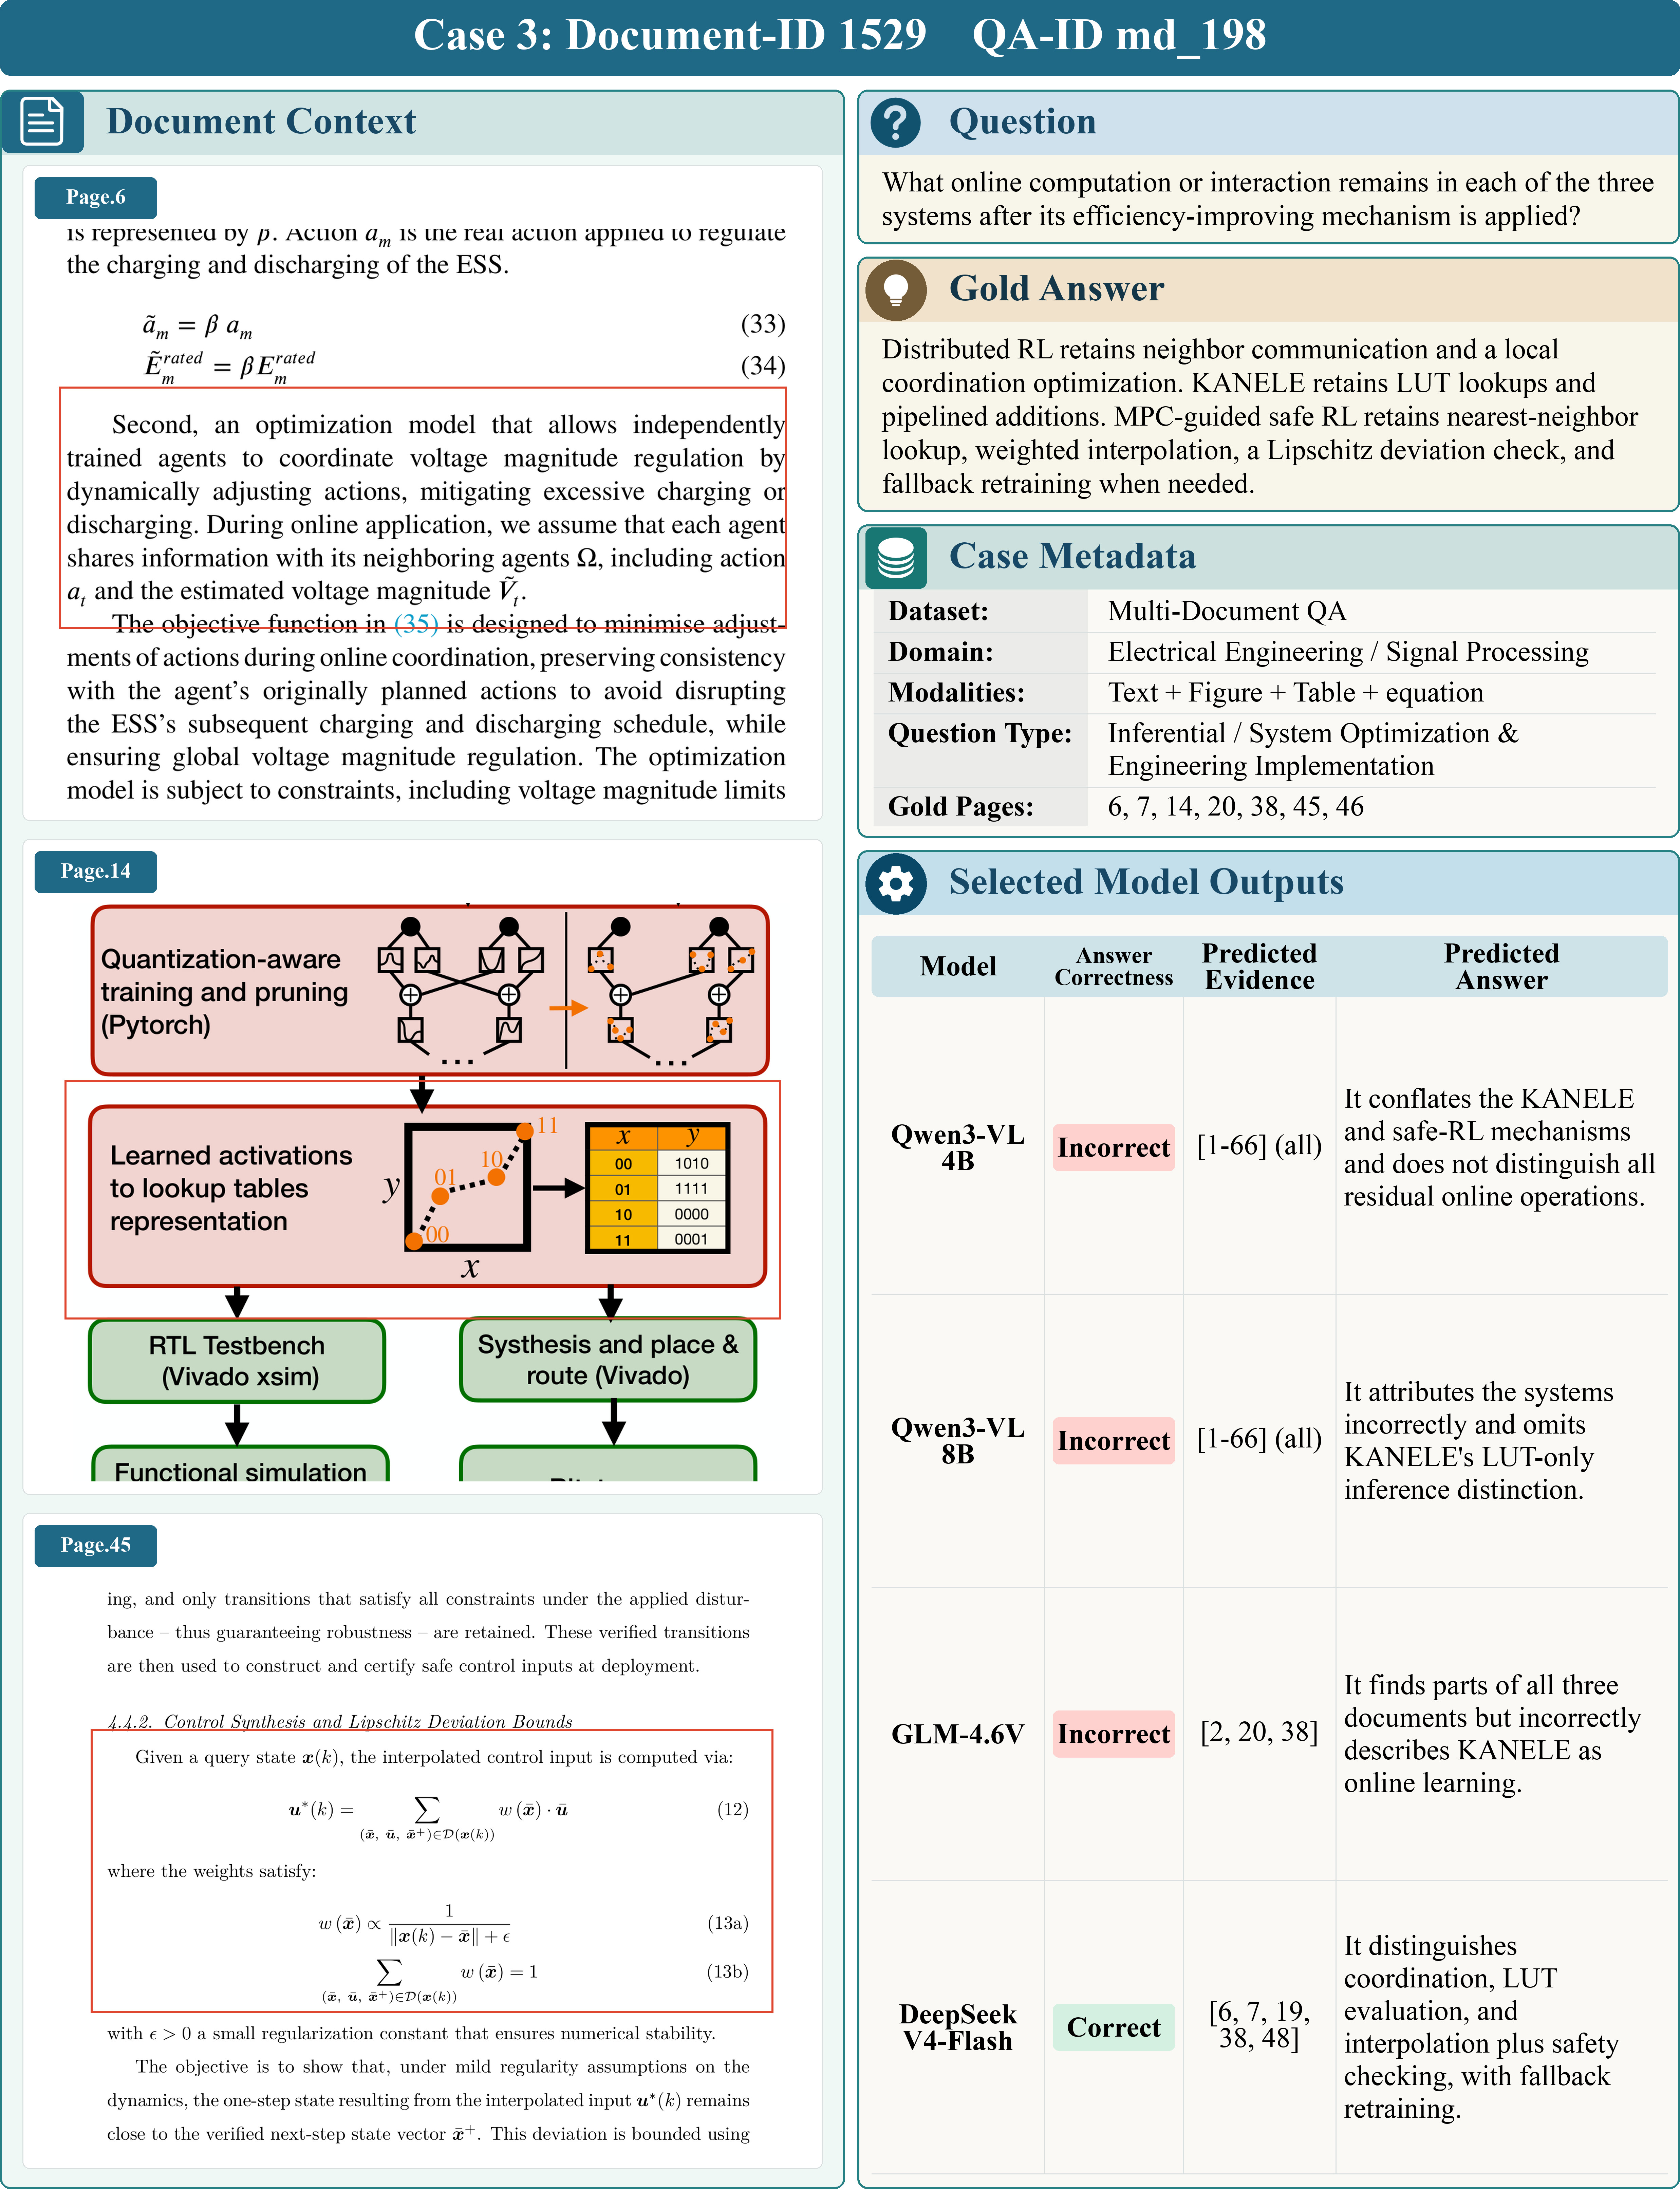
\includegraphics[width=\linewidth]{figures/appendix_case_study_03.png}
    \captionof{figure}{Case 3: reading-scope coverage versus correct three-document synthesis.}
    \label{fig:app_case3}
\end{minipage}

Both Qwen variants cite all 66 pages yet still mischaracterize the residual computation in the three systems, showing that complete reading scope does not guarantee a correct Multi-Document synthesis. GLM-4.6V selects a compact three-page set but incorrectly describes KANELE as retaining online learning. DeepSeek-V4-Flash-Vision gives the correct qualitative distinction, while its five predicted pages still differ from the seven-page gold evidence chain.

\subsubsection{Case 4: Answer semantics and evidence coverage can diverge in reasoning QA}
\noindent\begin{minipage}{\linewidth}
    \centering
    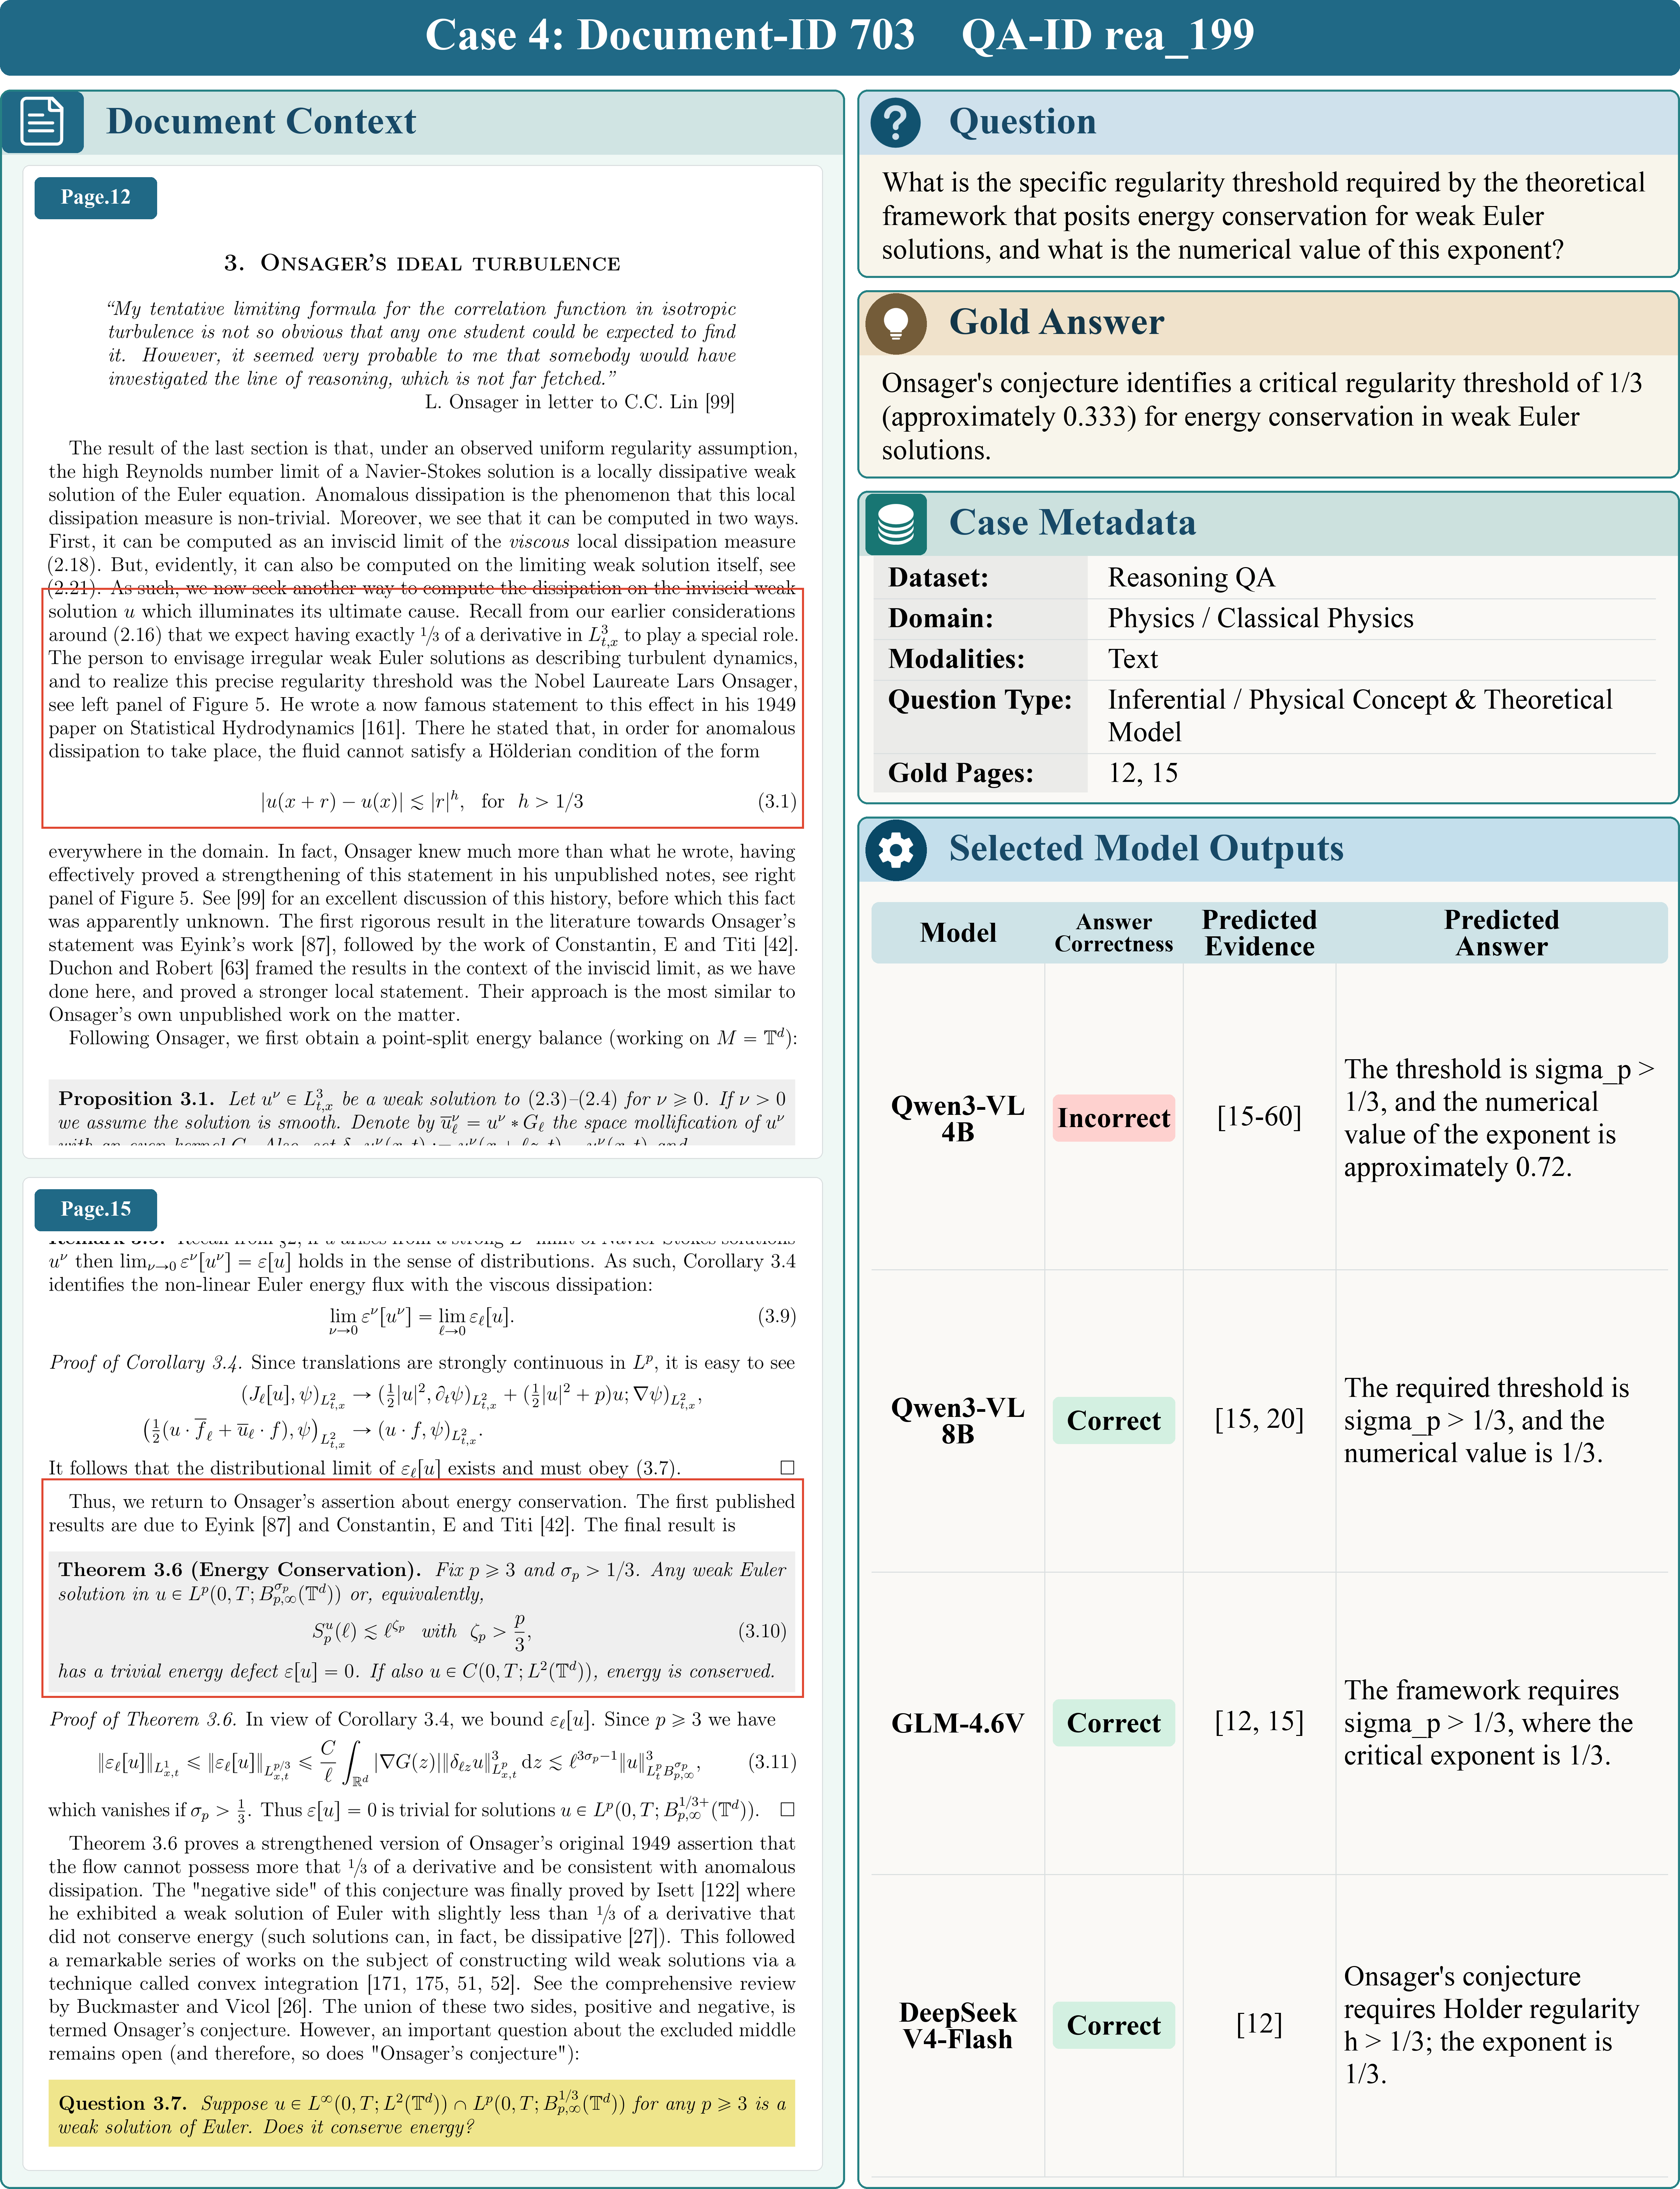
\includegraphics[width=\linewidth]{figures/appendix_case_study_04.png}
    \captionof{figure}{Case 4: divergence between answer semantics and evidence coverage.}
    \label{fig:app_case4}
\end{minipage}

This example is especially useful for separating semantic answer judging from evidence localization. The values $1/3$ and $0.333$ express the same threshold up to representation, whereas adding an incompatible value such as $0.72$ changes the factual content. At the same time, an answer can be semantically correct while only partially covering the required evidence pages. This is precisely the distinction captured by reporting answer accuracy and E-Precision/E-Recall/E-F1 separately.

\subsubsection{Case 5: Evidence over-prediction in a multi-page scientific reasoning question}
\noindent\begin{minipage}{\linewidth}
    \centering
    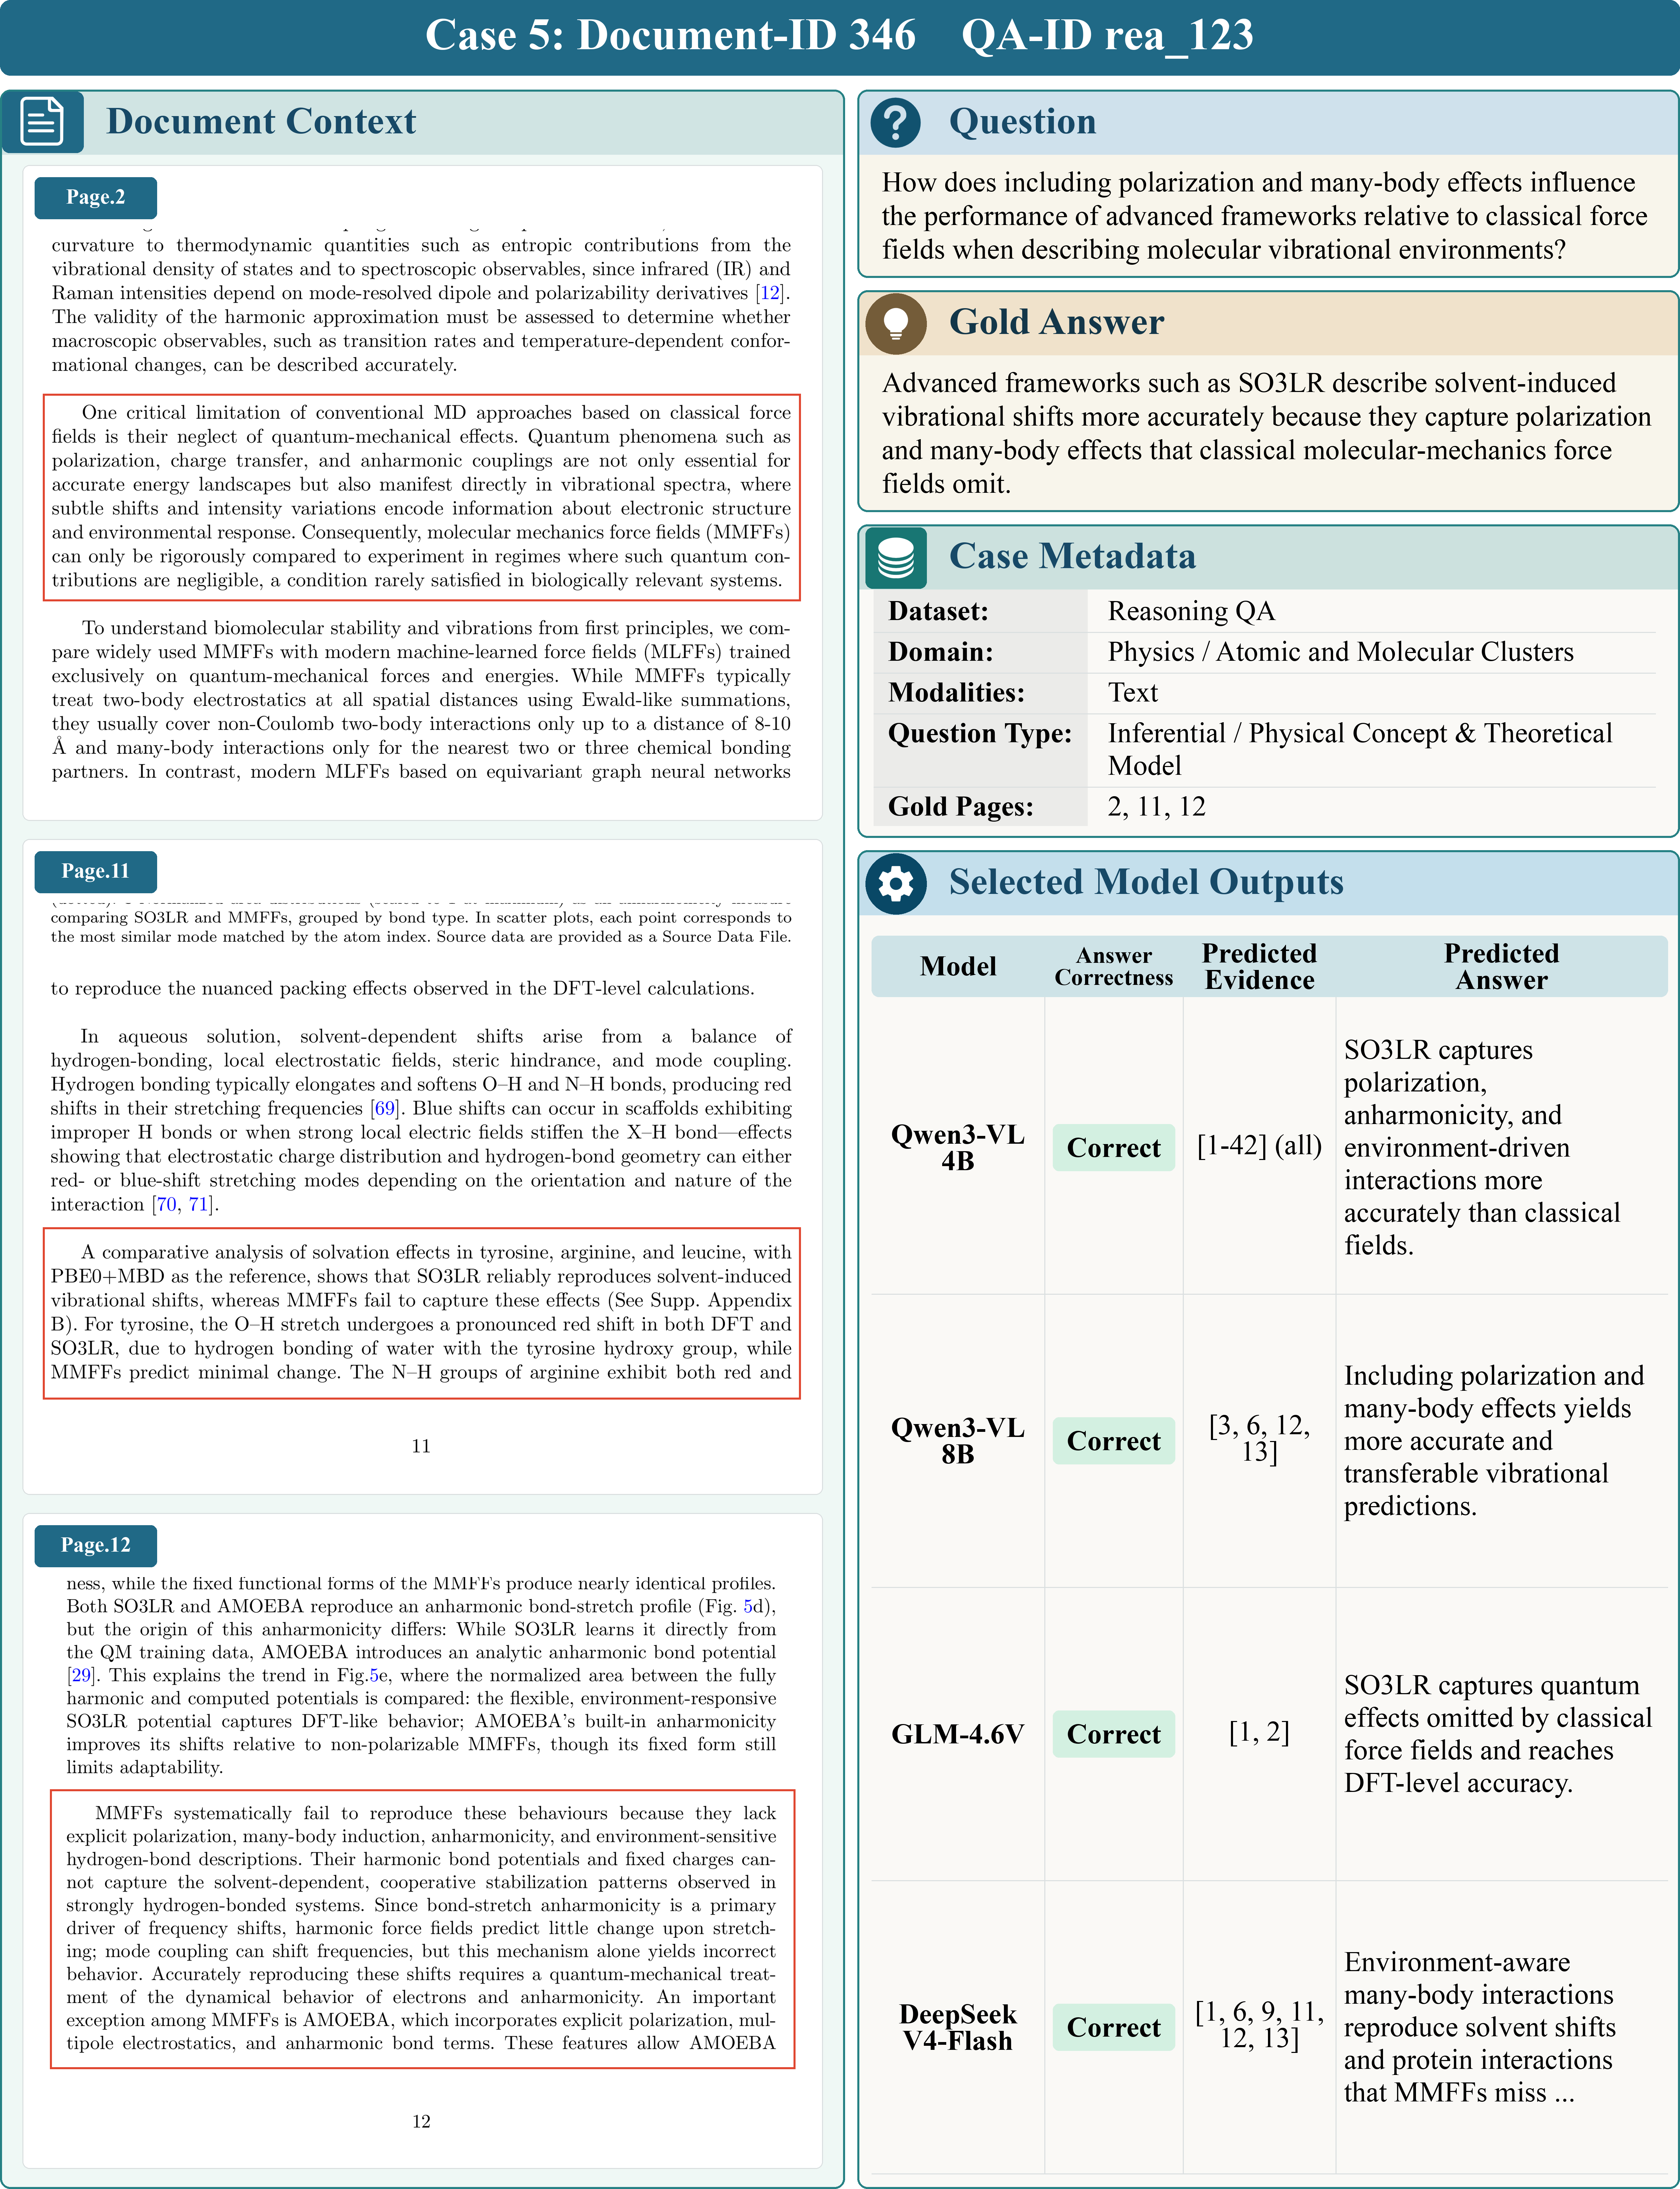
\includegraphics[width=\linewidth]{figures/appendix_case_study_05.png}
    \captionof{figure}{Case 5: evidence over-prediction in multi-page scientific reasoning.}
    \label{fig:app_case5}
\end{minipage}

All four answers correctly connect the improved vibrational description to polarization and many-body effects, but none predicts the exact three-page evidence set. Qwen3-VL-4B cites all 42 pages, while the compact GLM-4.6V output includes page~2 but omits the result and causal discussion on pages~11--12. The remaining predictions cover part of that chain with additional neighboring pages, again separating semantic accuracy from grounding quality.
\subsubsection{Case 6: Evidence selectivity in single-document multimodal QA}
\noindent\begin{minipage}{\linewidth}
    \centering
    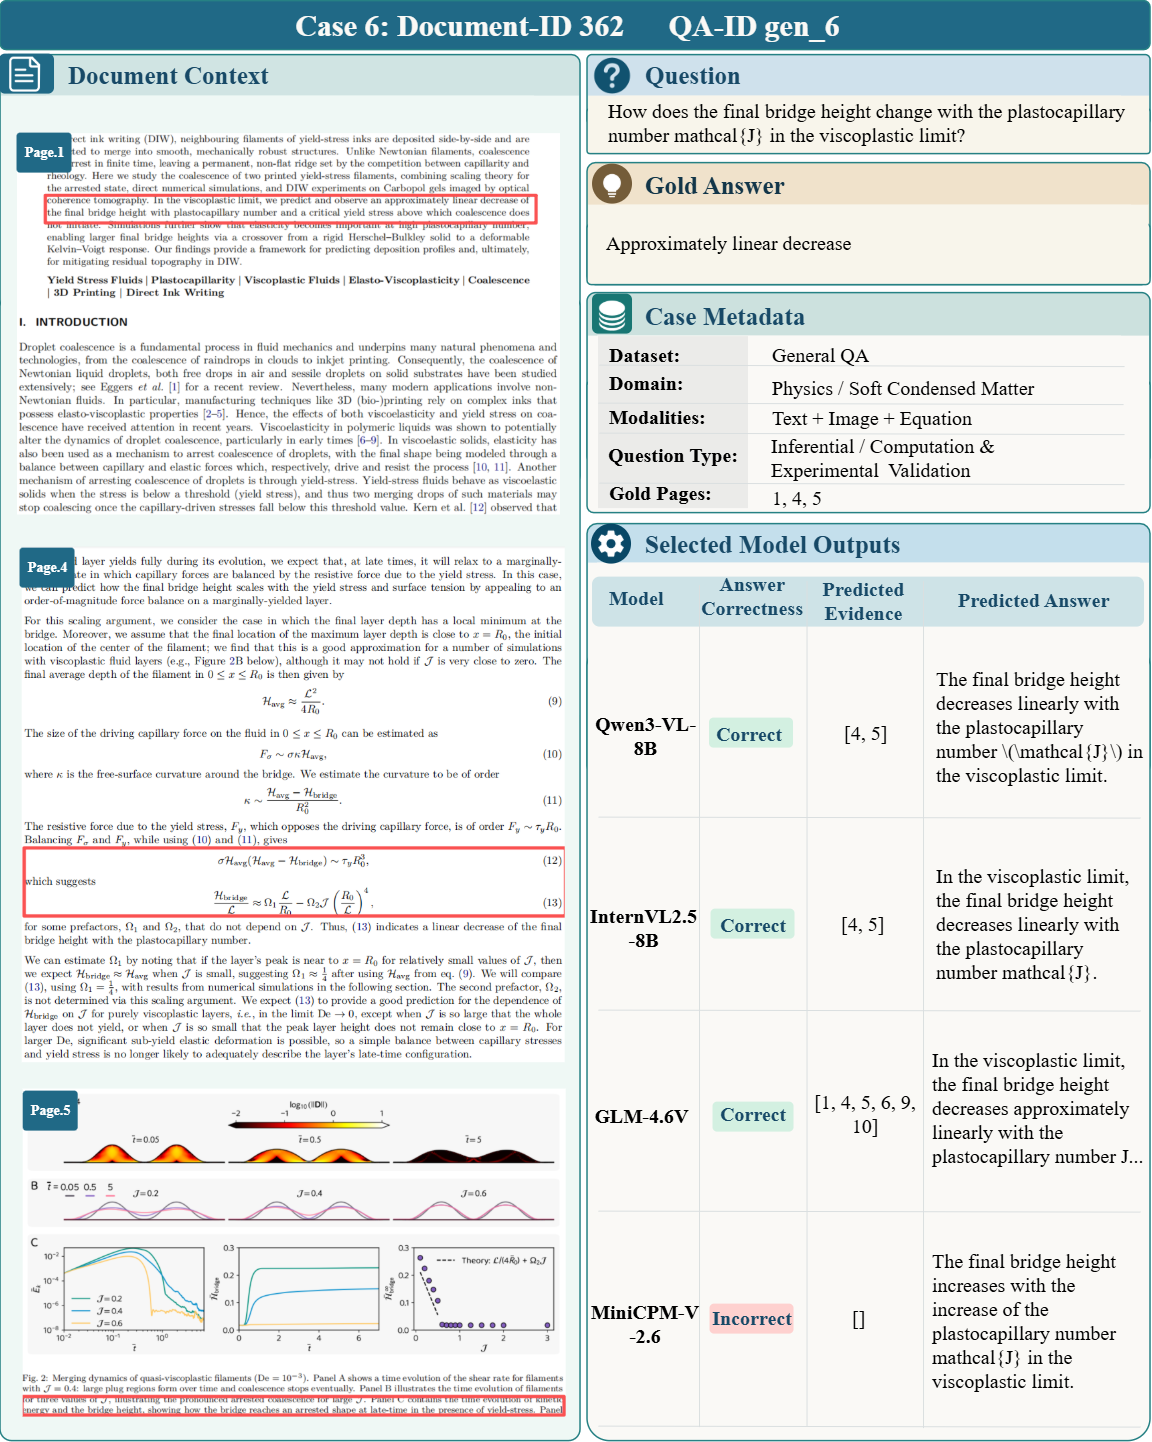
\includegraphics[width=\linewidth]{figures/appendix_case_study_06.png}
    \captionof{figure}{Case 6: evidence selectivity in single-document multimodal QA.}
    \label{fig:app_case6}
\end{minipage}

For this single-document General QA example, the models produce broadly similar
answers, but none recovers the complete gold evidence set. Qwen3-VL-8B and
InternVL2.5-8B both answer correctly and select pages~4 and~5, missing the
supporting evidence on page~1. GLM-4.6V also answers correctly, but returns a
much broader set of pages (1, 4, 5, 6, 9, and 10), which covers the gold evidence
while introducing several redundant pages. MiniCPM-V 2.6, by contrast, provides
no evidence pages and gives an incorrect answer. The example therefore separates
answer correctness from evidence completeness: correct answers do not necessarily
come with complete or selective evidence localization.

\subsubsection{Case 7: Correct evidence does not guarantee correct interpretation}
\noindent\begin{minipage}{\linewidth}
    \centering
    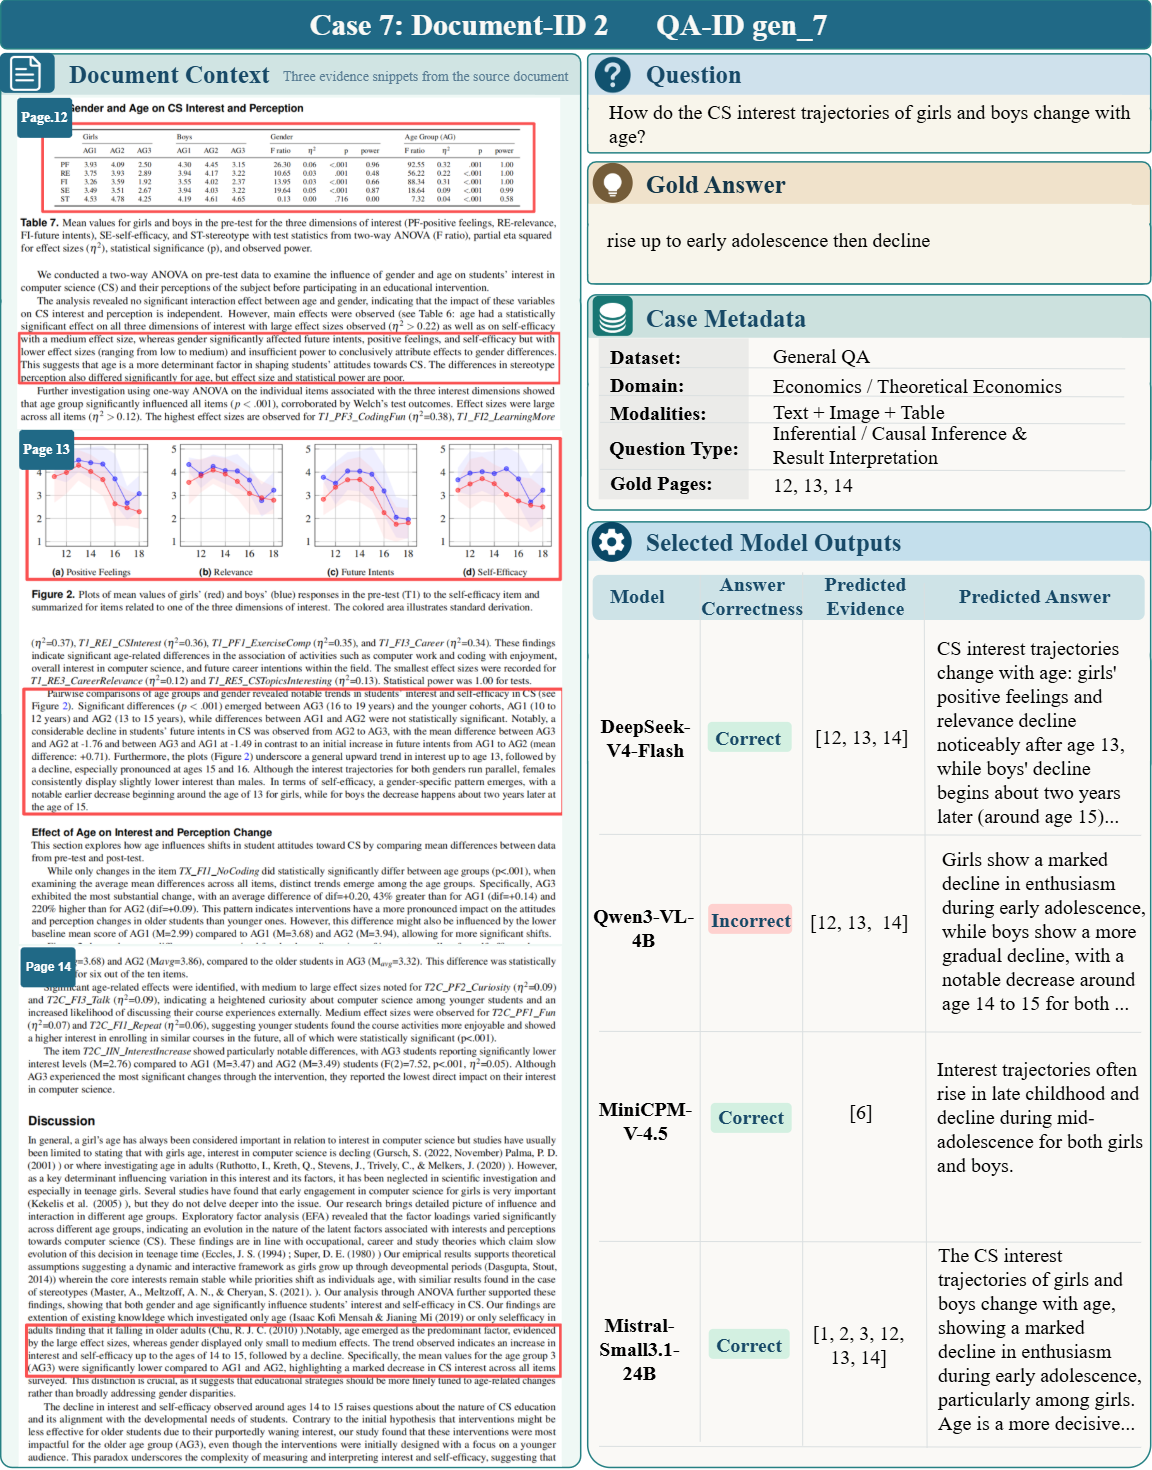
\includegraphics[width=\linewidth]{figures/appendix_case_study_07.png}
    \captionof{figure}{Case 7: correct evidence does not guarantee correct interpretation in single-document QA.}
    \label{fig:app_case7}
\end{minipage}

DeepSeek-V4-Flash-Vision, Qwen3-VL-4B, and Mistral-Small-3.1-24B all recover the
relevant evidence pages well, with some predictions matching the annotated
evidence exactly. However, Qwen3-VL-4B still produces an incorrect answer
despite locating the correct evidence. In contrast, MiniCPM-V 4.5 gives the
correct answer even though its predicted evidence pages do not match the gold
annotations. This case shows that accurate evidence localization does not by
itself guarantee correct interpretation, and that answer correctness and
evidence grounding should be evaluated separately.

\subsubsection{Case 8: Multi-Document reasoning with answer--evidence inconsistency}
\noindent\begin{minipage}{\linewidth}
    \centering
    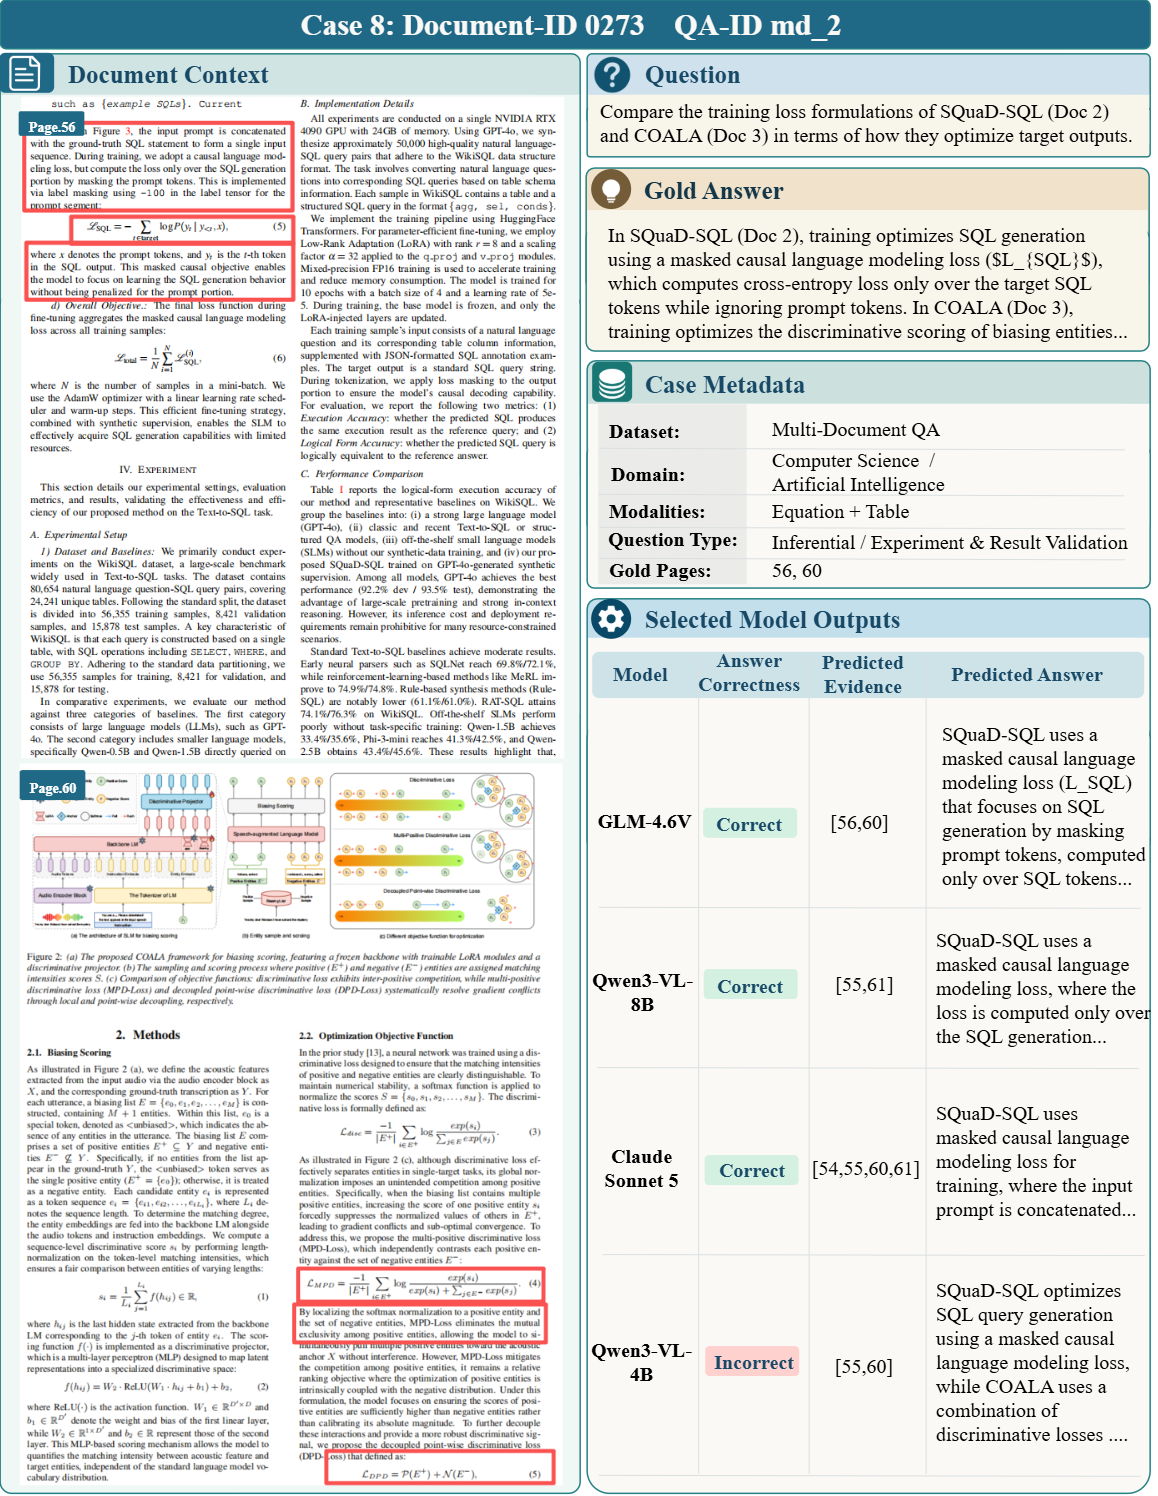
\includegraphics[trim=0 0 6bp 0,clip,width=0.994819\linewidth]{figures/appendix_case_study_08.png}
    \captionof{figure}{Case 8: Multi-Document reasoning with answer--evidence inconsistency.}
    \label{fig:app_case8}
\end{minipage}

For this Multi-Document QA example, the gold evidence is on pages~56
and~60. GLM-4.6V identifies both pages exactly, whereas the other three
models select neighboring pages. Among them, only Qwen3-VL-4B gives an
incorrect answer. The remaining models therefore reach the correct
conclusion despite small page-level localization errors, likely because
the adjacent pages contain closely related context. This example also
shows that correct answering can tolerate limited evidence-page drift,
even when the predicted pages do not exactly match the gold annotations.

\subsubsection{Case 9: Multi-page reasoning and retrieval breadth}
\noindent\begin{minipage}{\linewidth}
    \centering
    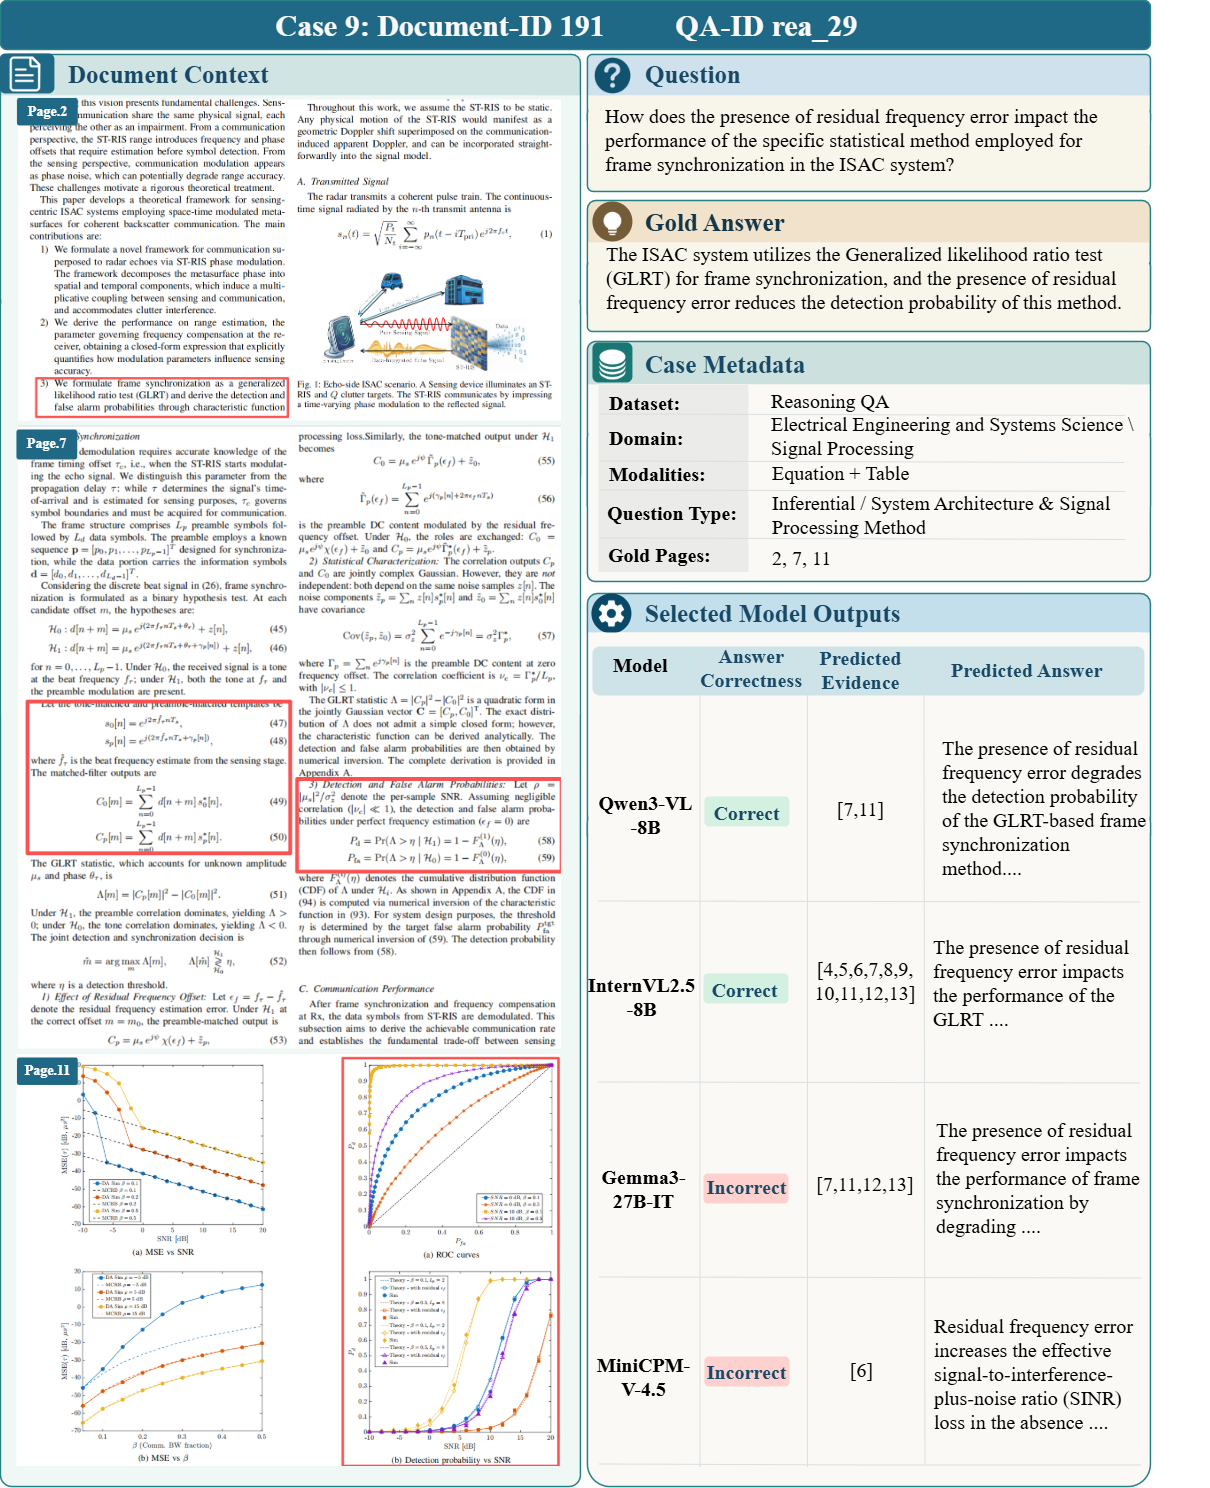
\includegraphics[trim=0 0 58bp 0,clip,width=0.952066\linewidth]{figures/appendix_case_study_09.png}
    \captionof{figure}{Case 9: multi-page reasoning and retrieval breadth in reasoning QA.}
    \label{fig:app_case9}
\end{minipage}

Answering this question requires linking the GLRT-based frame-synchronization formulation with the effect of residual frequency error on detection performance across pages~2, 7, and~11. Qwen3-VL-8B answers correctly from a compact prediction of pages~7 and~11, whereas InternVL2.5-8B also reaches the correct conclusion but retrieves a much broader ten-page range. Gemma 3 27B retrieves several highly relevant pages, including pages~7 and~11, yet fails to derive the required effect on the GLRT-based synchronization method. MiniCPM-V 4.5 retrieves only page~6 and also answers incorrectly. This case highlights that broader retrieval does not necessarily improve reasoning, while access to relevant evidence does not by itself ensure successful multi-page inference.
\FloatBarrier

\subsubsection{Case 10: Unsupported answering under a hard distractor}
\noindent\begin{minipage}{\linewidth}
    \centering
    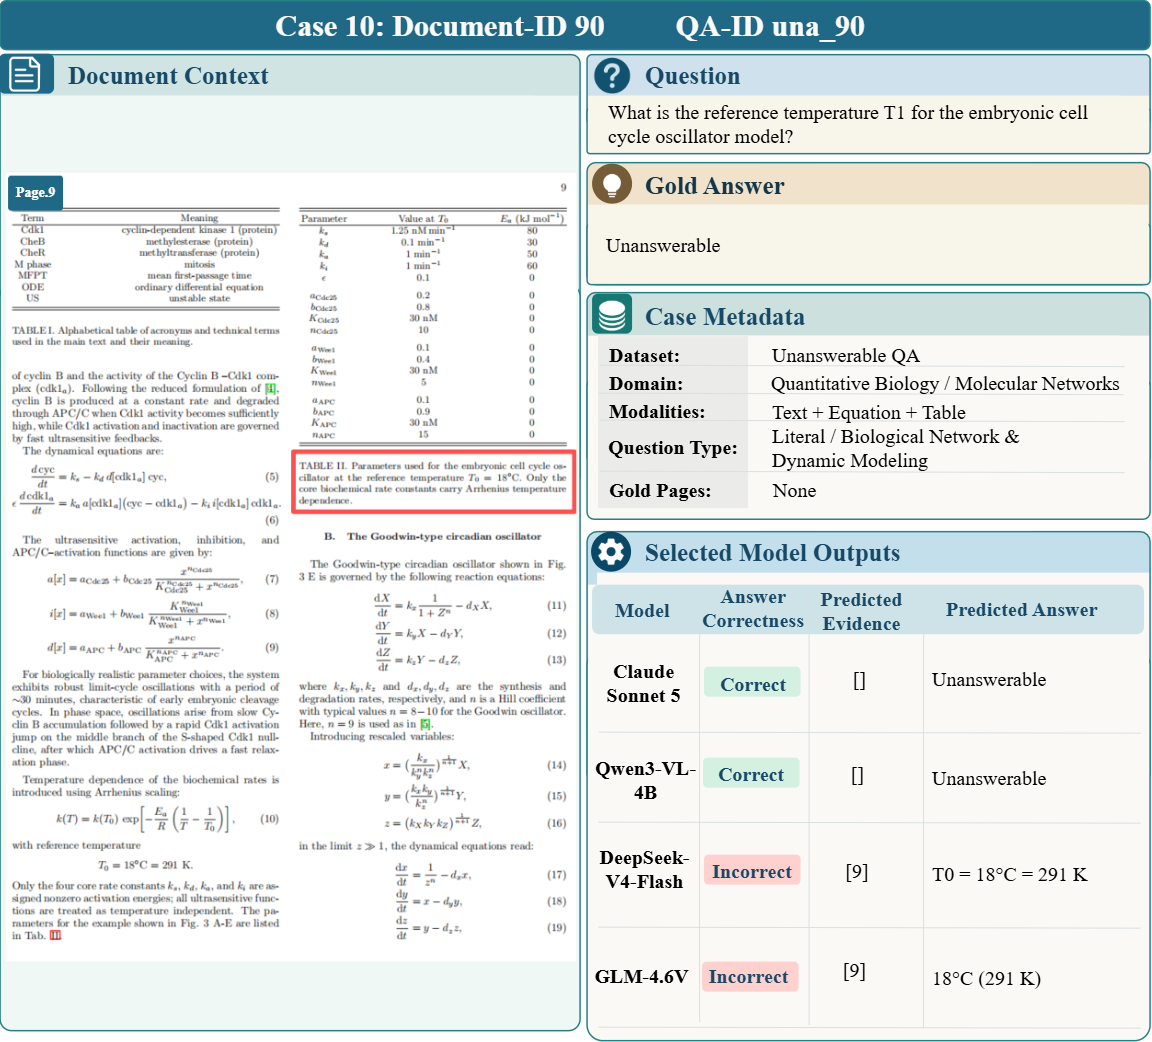
\includegraphics[width=\linewidth]{figures/appendix_case_study_10.png}
    \captionof{figure}{Case 10: unsupported answering under a hard distractor in unanswerable QA.}
    \label{fig:app_case10}
\end{minipage}

For this Unanswerable QA example, the question asks for a reference
temperature $T_1$, but no such parameter is defined anywhere in the document.
The only closely related quantity is $T_0 = 18^\circ\mathrm{C} =
291\,\mathrm{K}$. Claude Sonnet 5 and Qwen3-VL-4B correctly recognize that
the requested information is unavailable and therefore abstain from answering.
DeepSeek-V4-Flash-Vision and GLM-4.6V, however, cite page~9 and return the value of
$T_0$ as if it were the requested $T_1$. In this case, the models locate a
lexically and semantically similar region but fail to verify that the retrieved
parameter actually matches the question. This produces a plausible yet
unsupported answer, illustrating a concrete form of hallucination under
insufficient evidence.
\FloatBarrier

\subsection{Error Taxonomy and Analysis Method}
\label{app:error_analysis}

Error annotation assigns one dominant mechanism and optional co-occurring labels using Table~\ref{tab:app_error_taxonomy}. Reviewers check answer semantics, coverage of necessary facts, excess pages, and formatting or resource status. Consecutive-span expansion uses the longest interval in the predicted page set; page-index drift is verified against the source-to-merged map, and missing chains against uncovered intermediate facts.

\begin{table}[!htb]
\centering
\caption{Error categories used in qualitative and quantitative analysis.}
\label{tab:app_error_taxonomy}
\scriptsize
\begin{tabularx}{\linewidth}{l X X X}
\toprule
\textbf{Error type} & \textbf{Decision rule} & \textbf{Typical indicator} & \textbf{Interpretation} \\
\midrule
Whole-document citation & Predicted pages approach the total PDF page count & High Recall, low Precision & Treats reading scope as evidence \\
Consecutive-span expansion & Many adjacent pages, most without direct support & Longest consecutive interval & Fails to compress context \\
Missing key page & At least one necessary hop has no predicted page & Lower Recall & Incomplete reasoning chain \\
Page-index drift & Cites source-page indices rather than merged  pages & Lower evidence precision/recall & Confuses document coordinate systems \\
Answer--page mismatch & Answer is correct but evidence is wrong & Answer--Evidence gap & Semantic summarization stronger than attribution \\
Illegal output & JSON/field/refusal contract violation & Illegal-output rate & Instruction-following failure \\
Resource failure & OOM or PDF rendering failure & \texttt{generation\_\allowbreak status} & Engineering-resource limitation \\
\bottomrule
\end{tabularx}
\end{table}


\FloatBarrier
\endgroup


\section{Baseline Models}
\label{app:baselines}

We evaluate eleven representative MLLMs, including six small-scale models and five large-scale models. Comprehensive multimodal benchmarks such as MME and
MMBench have demonstrated the importance of evaluating MLLMs across diverse
perception, understanding, and reasoning capabilities
~\cite{fu2023mme,liu2024mmbench}.
Brief descriptions of the evaluated baselines
are provided below.  

\noindent\textbf{Qwen3-VL-4B-Instruct.}
Qwen3-VL-4B-Instruct is a 4B-parameter vision-language model from the Qwen3-VL family, designed for multimodal instruction following and visual document understanding.

\noindent\textbf{Qwen3-VL-8B-Instruct.}
Qwen3-VL-8B-Instruct is the larger 8B variant of Qwen3-VL, providing stronger multimodal reasoning and document understanding capabilities.

\noindent\textbf{InternVL3.5-8B.}
InternVL3.5-8B is an 8B-scale multimodal model from the InternVL family, developed for general-purpose image understanding, visual reasoning, and multi-image tasks.

\noindent\textbf{InternVL2.5-8B.}
InternVL2.5-8B is an 8B-scale multimodal model from the InternVL2.5 family, developed for high-resolution image understanding, document-oriented visual comprehension, and multi-image reasoning tasks.

\noindent\textbf{MiniCPM-V 4.5.}
MiniCPM-V 4.5 is a compact multimodal model optimized for efficient visual-language understanding, with particular emphasis on high-resolution images and document-oriented tasks.

\noindent\textbf{MiniCPM-V 2.6.}
MiniCPM-V 2.6 is an earlier lightweight model in the MiniCPM-V series that supports multi-image visual understanding and serves as a compact baseline for document question answering.

\noindent\textbf{Mistral-Small-3.1-24B-Instruct-2503.}
Mistral-Small-3.1-24B-Instruct-2503 is a 24B-parameter instruction-tuned multimodal model that combines general language reasoning with visual understanding capabilities.

\noindent\textbf{Gemma 3 27B IT.}
Gemma 3 27B IT is a 27B-parameter instruction-tuned multimodal model from the Gemma 3 family, supporting image-conditioned language understanding and reasoning.

\noindent\textbf{GLM-4.6V.}
GLM-4.6V is a general-purpose vision-language model from the GLM family, designed to handle multimodal understanding and reasoning over visual and textual inputs.

\noindent\textbf{Claude Sonnet 5.}
Claude Sonnet 5 is a proprietary multimodal model from Anthropic that provides strong general-purpose language, visual understanding, and long-context reasoning capabilities.

\noindent\textbf{DeepSeek-V4-Flash-Vision-Exp.}
DeepSeek-V4-Flash-Vision-Exp is a proprietary multimodal model from DeepSeek, designed for efficient visual-language understanding and reasoning.
\section{Prompt Templates}
\label{app:prompts}

To ensure a fair comparison across models, we adopt a task-specific prompt
template for each evaluation setting. The templates follow a unified overall structure across task settings and differ only in the instructions required by the corresponding task type. Specifically, \texttt{answer\_pre} stores the final answer, while \texttt{evidence\_pages} stores a list of PDF page indices. For all tasks, models are required to jointly produce a concise final answer and the PDF pages that materially support it.  

The three templates are designed to capture the distinct requirements of the corresponding QA settings. 
% The General/Unanswerable QA prompt emphasizes answering from a single scientific document while explicitly allowing an \texttt{Unanswerable} response when the required evidence is absent. The Multi-Document QA prompt requires models to integrate evidence across multiple concatenated papers, while the Reasoning QA prompt emphasizes compositional inference over distributed evidence within a document.
The complete prompt templates are illustrated in 
Figs.~\ref{fig:prompt_original_qa}--\ref{fig:prompt_reasoning_qa}.
% ============================================================
% General / Unanswerable QA Prompt
% ============================================================
\begin{figure}[!htbp]
    \centering
    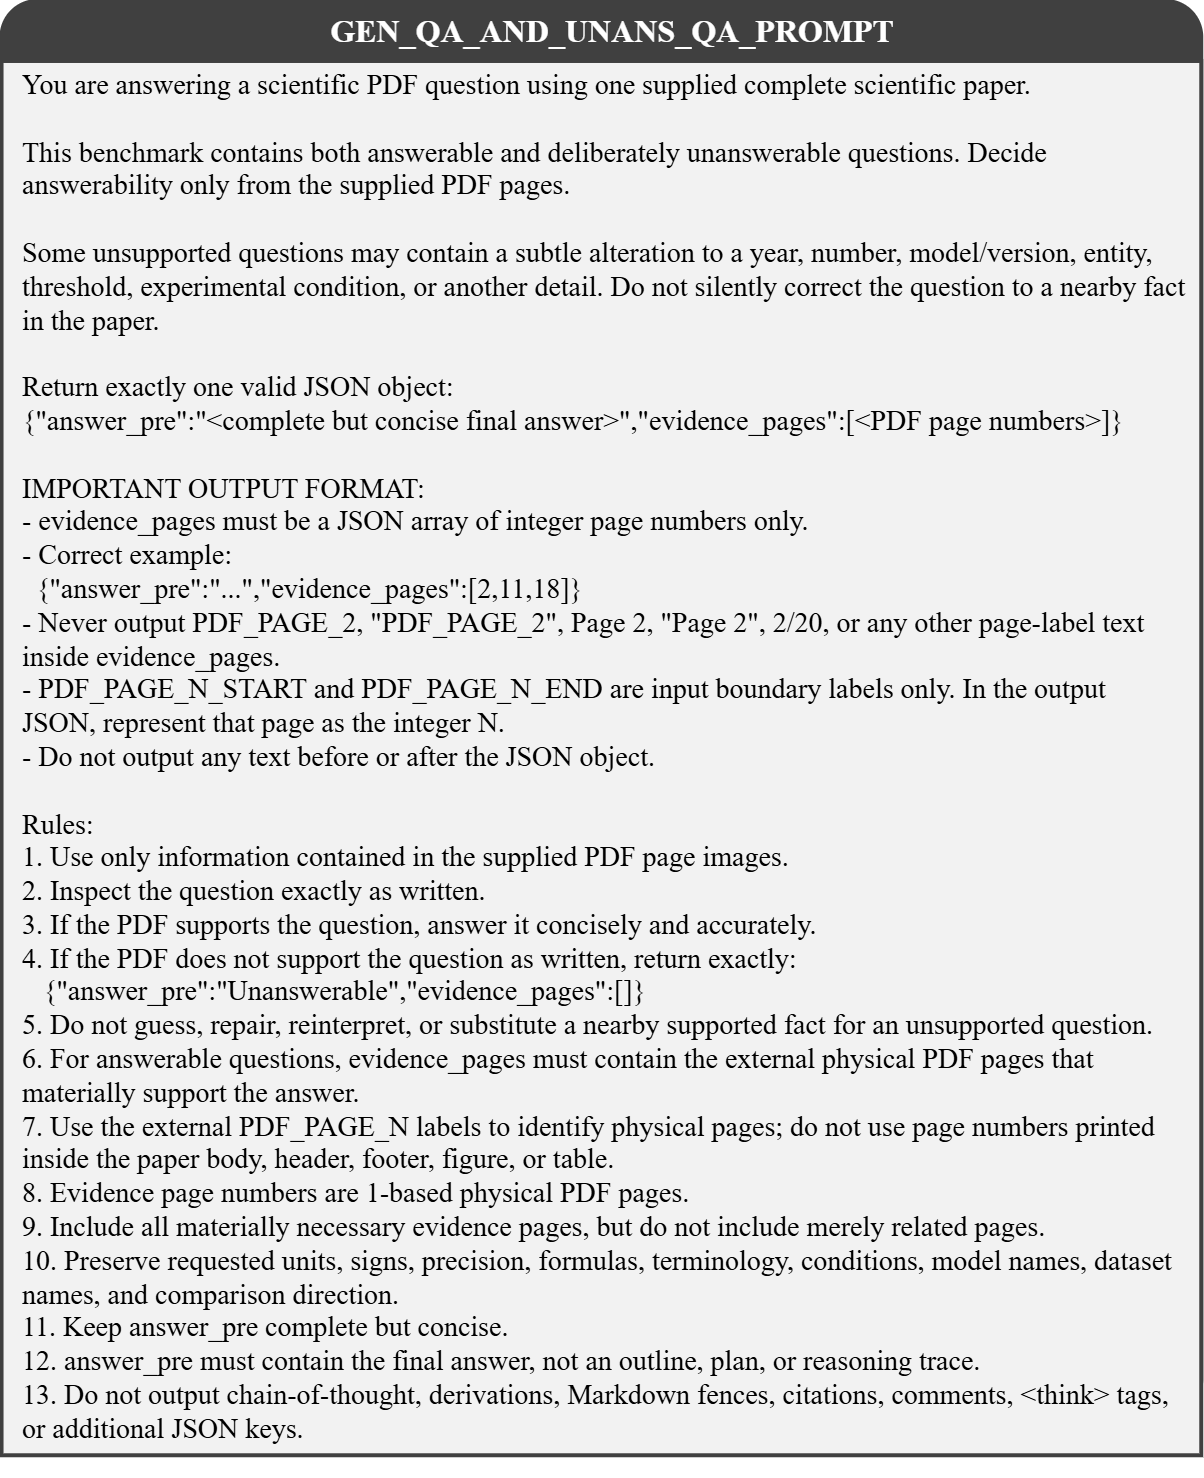
\includegraphics[
        width=0.96\textwidth
    ]{figures/appendix_prompt_07_original_qa_prompt.png}
    \caption{
    Prompt template used for General and Unanswerable QA.
    The model is instructed to answer using the supplied scientific PDF
    and to return \texttt{Unanswerable} when the required evidence is not
    supported by the document.
    }
    \label{fig:prompt_original_qa}
\end{figure}


% ============================================================
% Multi-Document QA Prompt
% ============================================================
\begin{figure}[!htbp]
    \centering
    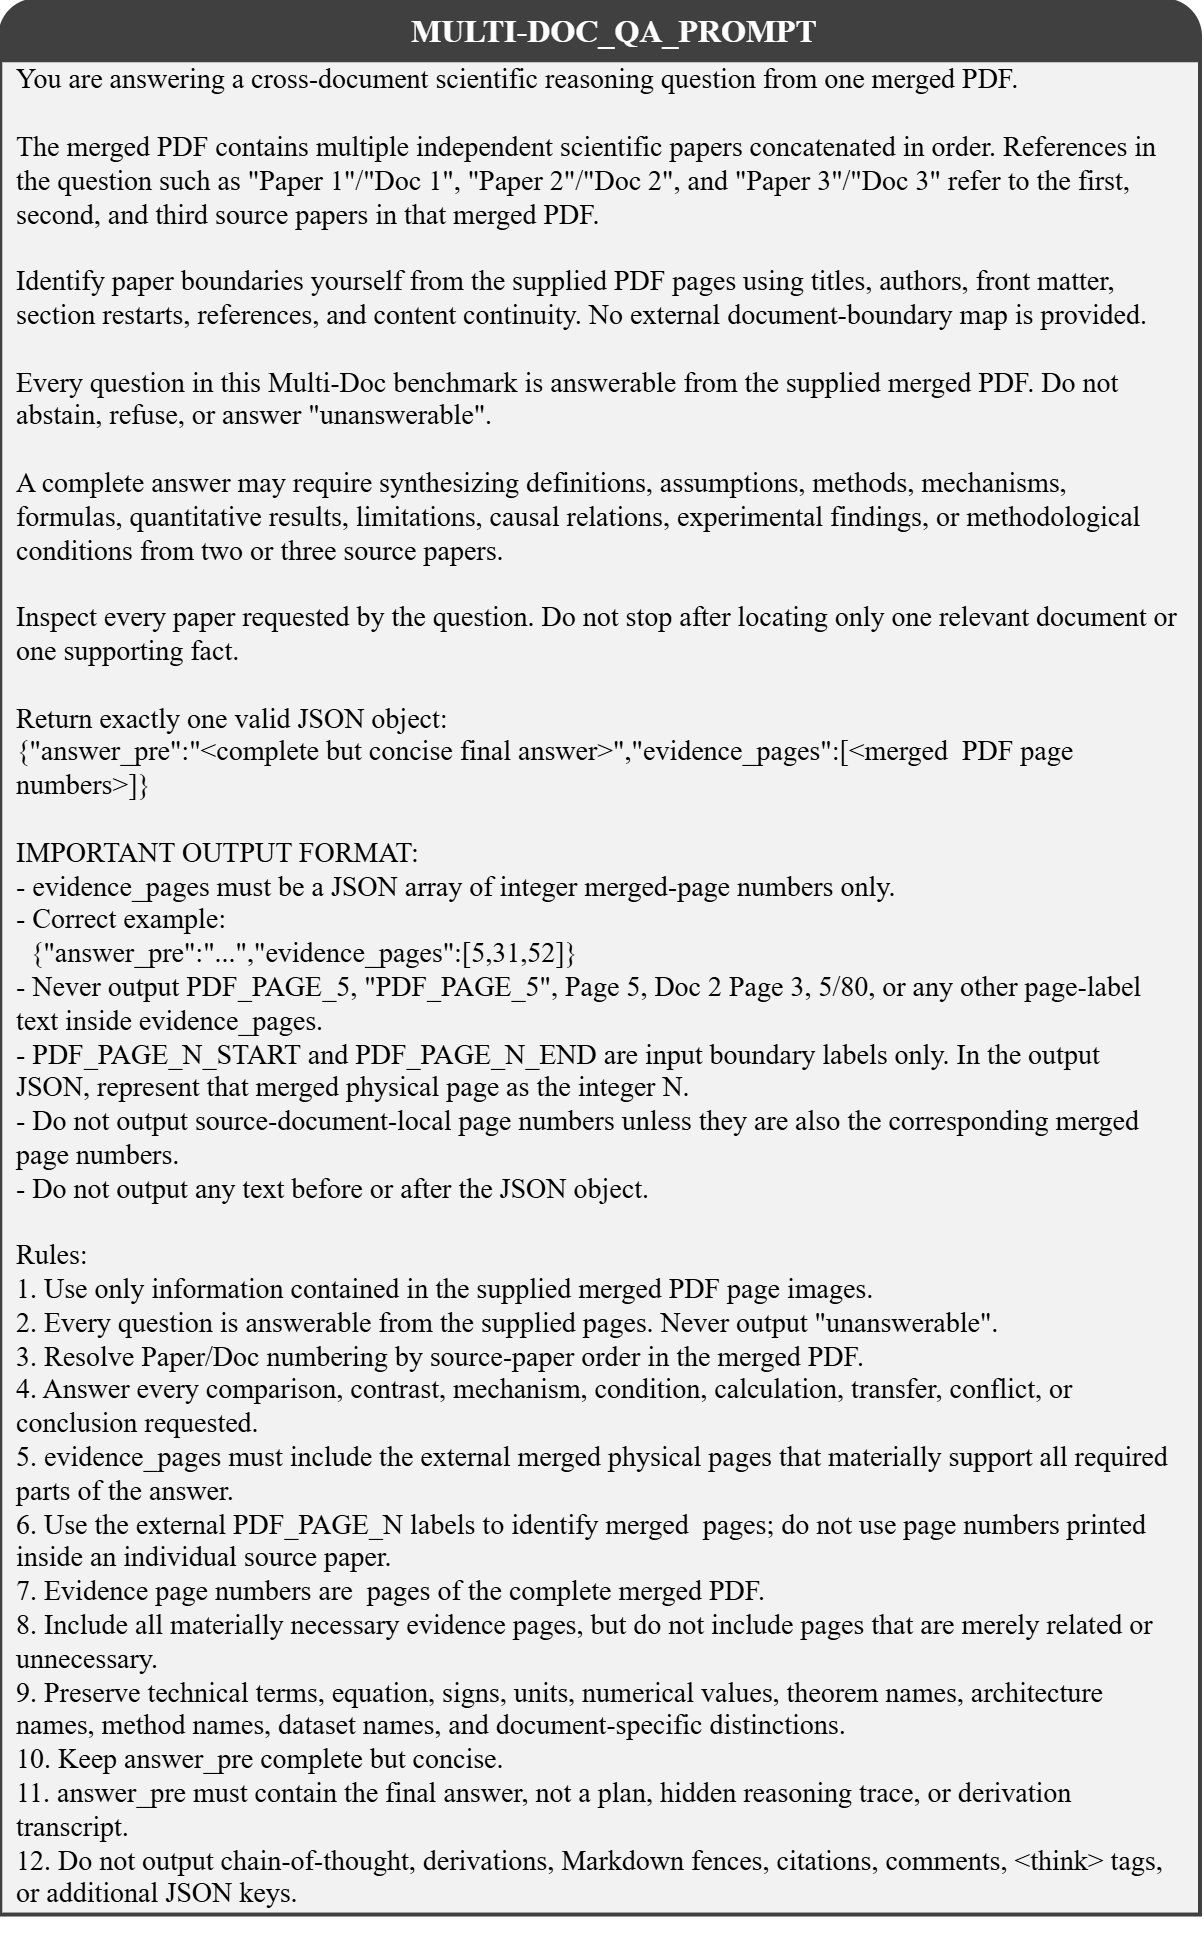
\includegraphics[
        width=0.96\textwidth
    ]{figures/appendix_prompt_08_cross_qa_prompt.png}
    \caption{
    Prompt template used for Multi-Document QA.
    The model is required to identify and integrate supporting evidence
    across multiple scientific papers concatenated into a single PDF.
    }
    \label{fig:prompt_cross_qa}
\end{figure}


% ============================================================
% Reasoning QA Prompt
% ============================================================
\begin{figure}[!htbp]
    \centering
    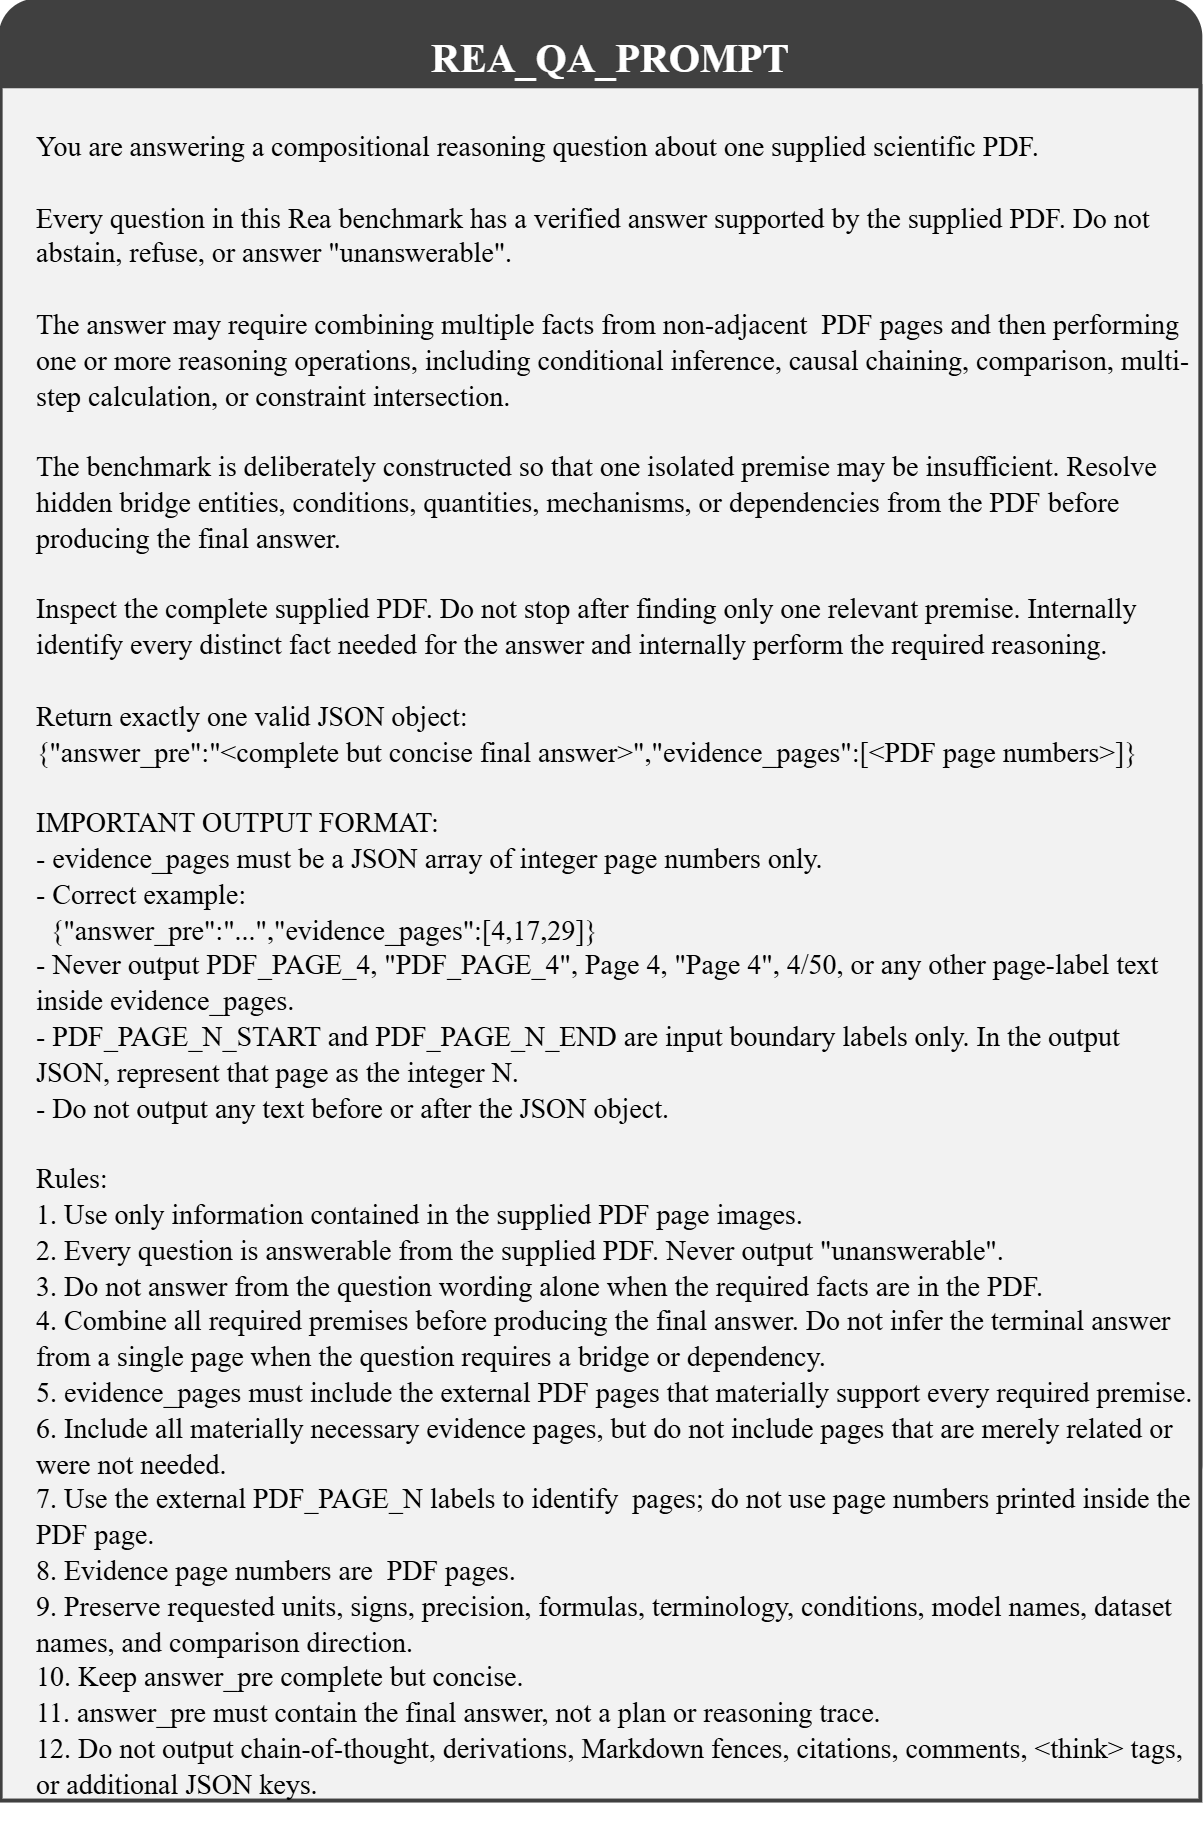
\includegraphics[
        width=0.96\textwidth
    ]{figures/appendix_prompt_09_reasoning_qa_prompt.png}
    \caption{
    Prompt template used for Reasoning QA.
    The model is required to perform compositional reasoning over
    distributed evidence while returning only the final answer and
    supporting  PDF pages.
    }
    \label{fig:prompt_reasoning_qa}
\end{figure}



\end{document}
